\documentclass[12pt,a4paper]{book}
\textwidth17cm
\textheight24.5cm
\oddsidemargin-0.5cm
\evensidemargin-0.5cm
\topmargin-1cm
\usepackage{natbib}
\setcounter{secnumdepth}{4}
\setcounter{tocdepth}{3}
\usepackage[bf]{caption}
\usepackage{listings}
\newcommand{\code}[1]{\texttt{#1}}
\newcommand{\CODE}[1]{\code{\MakeUppercase{#1}}} 
\newcommand{\cvar}[1]{\emph{#1}}
\newcommand{\tvar}[1]{<#1>}
%\usepackage{colortbl}
\usepackage[dvips]{color}
\usepackage{multicol}
\usepackage{multirow}
\usepackage{amsmath}
\usepackage{amssymb}
\usepackage[squaren]{SIunits}
\usepackage{ifpdf}
\usepackage[pdftex,colorlinks]{hyperref}
\usepackage{epsfig,colordvi}
\usepackage{longtable}
\newlength{\DUtablewidth} % internal use in tables
\usepackage[latin1]{inputenc}
\usepackage{tikz}
\usepackage{makeidx}
\usetikzlibrary{shapes,arrows}
\sloppy
%GREY FOR THE LSTLISTINGS
\definecolor{dgray}{gray}{0.9}
\setlength{\parindent}{0cm}
%\newcommand{\pfaw}[3]{\begin{tabular*}{9cm}{c}
%\psfig{figure=#1,angle=#2,width=#3cm}
%\end{tabular*}}
%%%%%%%%%%%%%%%%%%%%%%%%
%FOR USE WITH LSTLISTING
%%%%%%%%%%%%%%%%%%%%%%%%

  \lstset{basicstyle=\normalsize\ttfamily,
%           frame=lines,
           backgroundcolor=\color{dgray},
           breaklines=true,
           language=fortran,
           escapechar=?
           } 

%\newcommand{\pctthree}[3]{\begin{center}
%\begin{tabular*}{\textwidth}{c@{\extracolsep\fill}c}
%#1 & #2\\
%\multicolumn{2}{c}{#3}
%\end{tabular*}
%\end{center}}

\definecolor{mpggreen}{RGB}{0,119,112}
\newcommand{\mpimet}{Max Planck Institute for Meteorology}
\newcommand{\echamf}{\color{mpggreen}\texttt{ECHAM5}\color{black}}
\newcommand{\echam}{\color{mpggreen}\texttt{ECHAM6}\color{black}}
\newcommand{\echambw}{\texttt{ECHAM6}}
\newcommand{\blizzard}{{\it blizzard.dkrz.de}}
\newcommand{\thunder}{{\it thunder}}
\newcommand{\echamversion}{6.3.02}
\newcommand{\guideversion}{3.1}
\newcommand{\creationdate}{2015-08-27}
\newcommand{\inir}{{\tt /pool/data/ECHAM6/input/r0001\{RES\}/}}
\newcommand{\ini}{{\tt /pool/data/ECHAM6/input/r0001/}}
\newcommand{\ftswc}{F^{\top}_{\rm sw, clear}}
\newcommand{\fbswc}{F^{\bot}_{\rm sw, clear}}
\newcommand{\ftswa}{F^{\top}_{\rm sw, all}}
\newcommand{\fbswa}{F^{\bot}_{\rm sw, all}}
\newcommand{\ftlwc}{F^{\top}_{\rm lw, clear}}
\newcommand{\fblwc}{F^{\bot}_{\rm lw, clear}}
\newcommand{\ftlwa}{F^{\top}_{\rm lw, all}}
\newcommand{\fblwa}{F^{\bot}_{\rm lw, all}}
\newcommand{\ftswco}{F^{\top,0}_{\rm sw, clear}}
\newcommand{\fbswco}{F^{\bot,0}_{\rm sw, clear}}
\newcommand{\ftswao}{F^{\top,0}_{\rm sw, all}}
\newcommand{\fbswao}{F^{\bot,0}_{\rm sw, all}}
\newcommand{\ftlwco}{F^{\top,0}_{\rm lw, clear}}
\newcommand{\fblwco}{F^{\bot,0}_{\rm lw, clear}}
\newcommand{\ftlwao}{F^{\top,0}_{\rm lw, all}}
\newcommand{\fblwao}{F^{\bot,0}_{\rm lw, all}}
\newcommand{\ft}{F^{\top}}
\newcommand{\fb}{F^{\bot}}
\newcommand{\gm}{$\overline{\rm g}$}
\newcommand{\om}{\raisebox{-1.5ex}[1.5ex]{ --- }}
\newcommand{\cw}[1]{\textcolor{white}{#1}}
\newcommand{\tcr}[1]{\textcolor{red}{#1}}
\newcommand{\ditem}[1][]{\item[{#1}]\hfill}
\newcommand{\sm}{$\overline{\rm s}$}

% begin new commands for graphics
\newcommand{\arrays}{\renewcommand{\arraystretch}{0.5}}

\newcommand{\pfaw}[3]{\begin{tabular*}{9cm}{c}
\includegraphics[width=#3cm]{#1.pdf}
%\includegraphics[width=#3cm,angle=#2cm]{#1.pdf}
\end{tabular*}}

\newcommand{\pcttwo}[2]{\begin{center}
\begin{tabular*}{\textwidth}{c@{\extracolsep\fill}c}
#1 & #2\\
\end{tabular*}
\end{center}}

\newcommand{\pctthree}[3]{\begin{center}
\begin{tabular*}{\textwidth}{c@{\extracolsep\fill}cc}
#1 & #2 & #3\\
\end{tabular*}
\end{center}}

\newcommand{\pctthreetop}[3]{\begin{center}
\begin{tabular*}{\textwidth}{c@{\extracolsep\fill}c}
\multicolumn{2}{c}{#1}\\
#2 & #3\\
\end{tabular*}
\end{center}}

\newcommand{\pctfour}[4]{\arrays
\begin{center}
\begin{tabular*}{\textwidth}{c@{\extracolsep\fill}c}
#1 & #2\\
#3 & #4
\end{tabular*}
\end{center}}

\newcommand{\pctsix}[6]{\arrays
\begin{center}
\begin{tabular*}{\textwidth}{c@{\extracolsep\fill}c}
#1 & #2\\
#3 & #4\\
#5 & #6
\end{tabular*}
\end{center}}

\newcommand{\pctsixt}[6]{\arrays
\begin{center}
\begin{tabular*}{\textwidth}{c@{\extracolsep\fill}c@{\extracolsep\fill}c}
#1 & #2 & #3\\
#4 & #5 & #6
\end{tabular*}
\end{center}}

\newcommand{\pcteight}[8]{\arrays
\begin{center}
\begin{tabular*}{\textwidth}{c@{\extracolsep\fill}c}
#1 & #2\\
#3 & #4\\
#5 & #6\\
#7 & #8
\end{tabular*}
\end{center}}

%newcommands for putting view graphs into comptes rendus
\newcommand{\igcrtwzeonfozefizenirjs}[2]{\includegraphics[#1]{guide/cr/cr2014_05_09_rjs/#2}}

% end new commands for graphics

\makeindex

\begin{document}

\title{User manual for \echam}
\author{Sebastian Rast\thanks{Max
    Planck Institute of Meteorology, Hamburg, e--mail:
    sebastian.rast@mpimet.mpg.de}, Tobias Becker, Renate Brokopf, Suvarchal--Kumar
  Cheedela, \\
    Monika Esch, Irina Fast
    Veronika Gayler, Ingo Kirchner, \\Luis Kornblueh, Dagmar Popke, Andreas Rhodin,
    Hauke Schmidt, \\ Uwe Schulzweida, Aiko Voigt, Karl--Hermann Wieners}  
\date{\today, (\creationdate), version~echam--\echamversion--guide--\guideversion}

\frontmatter

\maketitle

%\rule{0cm}{1cm}
%\newpage


\tableofcontents

\listoftables
\newpage

\mainmatter
\chapter{Introduction}\label{capintroduction}
   The \echam{} model is a program for the
interactive calculation of the general circulation.
This manual contains a user guide of \echam{}
(chapter~\ref{capuserguide}) including a 
description of the compilation procedure on the 
supercomputer platform \blizzard{} at DKRZ Hamburg
(section~\ref{seccompiling}), a description of the input namelists
(section~\ref{secnamelist}), input files
(section~\ref{secinputfiles}), and ouput files
(section~\ref{secoutputfiles}), a description of example run scripts
(section~\ref{secrunscripts}), and postprocessing scripts
(section~\ref{secpostprocessing}). 
We restrict our description to the supercomputer platform 
\blizzard{} at DKRZ in Hamburg. Performing a simulation on other
computer platforms requires the same input data, but the compiling
procedure and the 
directory structure for output in particular, will be
different.

Chapter~\ref{captechguide} contains a short description of the code of
\echam{} and is intended to be a guide for people who work with the
source code of the atmosphere part of \echam. An introduction to the
\echam--code 
with explanations will become available in form of a lecture soon (``Using
and programming \echam{} --- a first introduction''). 

This description is valid for version echam--\echamversion.


\chapter{User guide}\label{capuserguide}

  \section[Compiling \echambw]{Compiling \echam}\label{seccompiling}
     \input{guide/ECHAM.guide.compiling}

  \section[Running \echambw]{Running \echam}\label{secrunning}
     The executable\index{executable echam6} is called {\tt echam6} and is put into {\tt
  echam-$<$tag\_number$>$/bin}. The actual command to call the
executable depends on the computer system. On the supercomputer
platform \blizzard{} at DKRZ, the command would be {\tt poe echam6}, on
Linux platforms you can use {\tt mpirun} in order to call a parallel
program. The {\tt echam6} command itself can take the arguments {\tt
  -i} or {\tt --init} that both have the same effect. This argument
forces an initial run and overrides any namelist setting in this respect. It is
therefore possible to use this command line option to perform a chain
job in which the subsequent calls of {\tt echam6} perform restarts
except the initial call for which the {\tt -i} or {\tt --init} option
has to be used. In such a case, the namelist for the first and
subsequent calls of {\tt echam6} can be identical although the first
call is an initial run and the subsequent calls are restarts. See
also the description of the {\tt lresume}
\index{namelist variables!lresume} namelist--variable in 
Tab.~\ref{tabrunctl}. 


  \section{Input namelists}\label{secnamelist}
     \subsection{Input namelists in file {\tt namelist.echam}}
  In Fortran, you can provide the values of input variables that are
  organized in
  namelists, specifying name and value of each variable. Several
  namelists are used to specify the input of \echam. Some of the
  namelists are for the atmospheric part and have to be written into
  the file {\tt namelist.echam}, others determine input variables of
  the land surface model JSBACH and have to be written into {\tt
    namelist.jsbach}. The atmospheric part can accept the following
  namelists in {\tt namelist.echam} (alphabetical order):

\begin{description}
  \item[{\tt cfdiagctl}:] \index{namelists!cfdiagctl}CFMIP2 station
    diagnostics. 
  \item[{\tt co2ctl}:] \index{namelists!co2ctl}interactive CO$_2$
    budget calculation. 
  \item[{\tt columnctl}:] \index{namelists!columnctl}single column model. 
  \item[{\tt cospctl}:] \index{namelists!cospctl}controls the COSP
    satellite simulator 
  \item[{\tt cospofflctl}:] \index{namelists!cospofflctl}namelist
    group for offline COSP 
    calculation. Offline means that data from files are read and no
    simulation of the general circulation takes place.
  \item[{\tt debugsctl}:] \index{namelists!debugsctl}creates a stream
    for grid point variables 
    that can be written to output easily (for debugging).
  \item[{\tt dyctl}:] \index{namelists!dynctl}parameters for
    atmosphere dynamics. 
  \item[{\tt ensctl}:] \index{namelists!ensctl}generate forecast ensembles.
  \item[{\tt gwsctl}:] \index{namelists!gwsctl}gravity wave parameterisation.
  \item[{\tt hratesctl}:] \index{namelists!hratesctl}diagnostic of
    heating rates. 
  \item[{\tt mvstreamctl}:] \index{namelists!mvstreamctl}variables
    controlling output of mean 
    values.
  \item[{\tt ndgctl}:] \index{namelists!ndgctl}variables which are
    related to the nudging of 
    the model, i.e.~to the relaxation method constraining the
    meteorological variables divergence, 
    vorticity, temperature and pressure to externally given values.
  \item[{\tt new\_tracer}:] \index{namelists!new\_tracer}new tracers
    can be introduced by the use of 
    this namelist group.
  \item[{\tt nmictl}:] \index{namelists!nmictl}normal mode analysis of waves.
  \item[{\tt parctl}:] \index{namelists!parctl}parameters concerning
    the parallel 
    configuration of model. 
  \item[{\tt physctl}:] \index{namelists!physctl}variables related to
    the physics calculation 
    like switching on/off radiation, diffusion,
  convection, surface exchange, \dots
  \item[{\tt radctl}:] \index{namelists!radctl}variables for
    controlling the radiation calculation. 
  \item[{\tt runctl}:] \index{namelists!runctl}contains variables
    concerning the start and the end 
  of a simulation.
  \item[{\tt set\_stream}:] \index{namelists!set\_stream}set the
    properties of an existing stream 
    by this namelist
  \item[{\tt set\_stream\_element}:]
    \index{namelists!set\_stream\_element}set stream element
    properties of 
    an existing stream element by namelist.
  \item[{\tt set\_tracer}:] \index{namelists!set\_tracer}this namelist
    group helps to set tracer 
    properties if they are created by some (sub)model.
  \item[{\tt stationctl}:] \index{namelists!stationctl}high frequency
    output at the location of 
    various sites including profiles.
  \item[{\tt submdiagctl}:] \index{namelists!submdiagctl}submodel diagnostics.
  \item[{\tt submodelctl}:] \index{namelists!submodelctl}namelists for
    registration of submodels in 
    \echam.
  \item[{\tt tdiagctl}:] \index{namelists!tdiagctl}tendency diagnostic.
\end{description}

The syntax for each namelist in {\tt namelist.echam} is
\index{namelist syntax}:
\begin{lstlisting}[caption= namelist syntax]
  & <namelist name>
    <varname> = <value>
  /
\end{lstlisting}

{\bf Remark:} The mere presence of a certain variable in a certain
namelist does not mean that the action associated with this variable
really works properly or works at all.

Variables describing repeated events have a special format (type
``special'' in the 
following tables\index{special format}): \newline
{\tt \{interval\}, \{unit\}, \{adjustment\}, \{offset\}}\newline
where {\tt \{interval\}} is a positive integer number, {\tt \{unit\}}
is one of {\tt 'steps'}, {\tt 'seconds'}, {\tt 'minutes'}, {\tt
  'hours'}, {\tt 'days'}, {\tt 'months'}, {\tt 'years'}, {\tt \{adjustment\}} is
one of {\tt 'first'}, {\tt 'last'}, {\tt 'exact'}, {\tt 'off'}, and {\tt
  \{offset\}} is an integer number giving the offset with respect to
the initial date of the simulation in seconds. A detailed description
of the control of time events can be found in the 
lecture ``Using and programming \echam{} --- a first introduction''
by S.~Rast. The variable list is given in
alphabetical order even if the most important variables are not at the
first place in this case.

\subsubsection{Namelist {\tt cfdiagctl}\index{namelists!cfdiagctl}}\label{seccfdiagctl}

This namelists contains only one parameter to switch on or off the
CFMIP2 diagnostics of 3--dimensional fluxes.

\setlength{\LTcapwidth}{\textwidth}
\setlength{\LTleft}{0pt}\setlength{\LTright}{0pt}

\begin{longtable}{l@{\extracolsep\fill}lp{5.0cm}p{3.0cm}}
\hline\hline\caption[Namelist {\tt cfdiagctl}]{Namelist
  {\tt cfdiagctl}}\\\hline\label{tabcfdiagctl}
\endfirsthead
\caption[]{{\tt cfdiagctl} --- continued}\\\hline
\endhead
\hline\multicolumn{4}{r}{\slshape table continued on next page}\\
\endfoot
\hline %\multicolumn{4}{r}{end of table}
\endlastfoot
Variable & type & Explanation & default \\\hline
{\tt locfdiag}\index{namelist variables!locfdiag} & logical & switches on/off CFMIP2 diagnostic output of
convective mass flux and 3-D radiation fluxes & {\tt .FALSE.} \\\hline
\end{longtable}
\subsubsection{Namelist {\tt co2ctl}\index{namelists!co2ctl}}\label{secco2ctl}

This namelist controls the behaviour of the CO$_2$ submodel. This
submodel is not a simple submodel like the transport of some gas phase
species would be because the CO$_2$ module interacts with the JSBACH
surface and vegetation model. In this namelist, the behaviour of the
CO$_2$ submodel in the atmosphere simulated by \echam{} and the
interaction with the ocean and soil simulated by JSBACH can be controlled.


\setlength{\LTcapwidth}{\textwidth}
\setlength{\LTleft}{0pt}\setlength{\LTright}{0pt}

\begin{longtable}{l@{\extracolsep\fill}lp{5.0cm}p{3.0cm}}
\hline\hline\caption[Namelist {\tt co2ctl}]{Namelist
  {\tt co2ctl}}\\\hline\label{tabco2ctl}
\endfirsthead
\caption[]{{\tt co2ctl} --- continued}\\\hline
\endhead
\hline\multicolumn{4}{r}{\slshape table continued on next page}\\
\endfoot
\hline %\multicolumn{4}{r}{end of table}
\endlastfoot
Variable & type & Explanation & default \\\hline
{\tt lco2\_flxcor}\index{namelist variables!lco2\_flxcor} 
& logical & switches on/off flux correction for
  exact mass balance & {\tt .TRUE.} \\
{\tt lco2\_mixpbl}\index{namelist variables!lco2\_mixpbl}
 & logical & switches on/off CO$_2$ mixing in
  planetary boundary layer & {\tt .TRUE.} \\
{\tt lco2\_2perc}\index{namelist variables!lco2\_2perc} 
& logical & switches on/off limitation of relative CO$_2$
  tendency to 2\% & {\tt .FALSE.} \\
{\tt lco2\_emis}\index{namelist variables!lco2\_emis} 
& logical & switches on/off reading prescribed CO$_2$
  emissions from a file & {\tt .FALSE.} \\
{\tt lco2\_clim}\index{namelist variables!lco2\_clim} 
& logical & switches on/off treating the CO$_2$
  concentration as a climatological quantity not being transported
  & {\tt .FALSE.} \\
{\tt lco2\_scenario}\index{namelist variables!lco2\_scenario} 
& logical & switches on/off reading CO$_2$
  concentrations from a certain greenhouse gas scenario
  & {\tt .FALSE.} but {\tt .TRUE.} if {\tt ighg=1} and {\tt lco2=.FALSE.}\\

\hline 
\end{longtable}


\subsubsection{Namelist {\tt columnctl}\index{namelists!columnctl}}\label{seccolumnctl}

This namelist controls the behaviour of the single column model. A more
detailed description of the single column model can be found in
section~\ref{secscm}. Here, we only present the namelist.

\setlength{\LTcapwidth}{\textwidth}
\setlength{\LTleft}{0pt}\setlength{\LTright}{0pt}

\begin{longtable}{l@{\extracolsep\fill}lp{5.0cm}p{3.0cm}}
\hline\hline\caption[Namelist {\tt columnctl}]{Namelist
  {\tt columnctl}}\\\hline\label{tabcolumnctl}
\endfirsthead
\caption[]{{\tt columnctl} --- continued}\\\hline
\endhead
\hline\multicolumn{4}{r}{\slshape table continued on next page}\\
\endfoot
\hline %\multicolumn{4}{r}{end of table}
\endlastfoot
variable & type & explanation & default \\\hline
{\tt forcingfile(32)}\index{namelist variables!forcingfile}
    &character       &name of the forcing file   &   ---   \\ 
 
{\tt mld}\index{namelist variables!mld} 
 & real & depth of mixed layer in metres & {\tt 10}\\
{\tt ml\_input}\index{namelist variables!ml\_input}
 & logical & {\tt ml\_input=.true.}: initial
temperature of mixed layer ocean is set to the value of the surface
temperature of the forcing file. {\tt ml\_input=.false.}: the sea
surface temperature is set to the value
given in the \echam{} sst file for the respective column & {\tt .false.}\\
{\tt nfor\_div(2)}\index{namelist variables!nfor\_div}
       &integer & option array describing the
treatment of the divergence of the wind field. The option array consists of
$\{i_{\rm set},i_{\rm cycle}\}$ as described in section~\ref{secforcing}. & {\tt (/0,0/)} \\
{\tt nfor\_lhf(2)}\index{namelist variables!nfor\_lhf}
       &integer & option array describing the
treatment of the latent heat flux. The option array consists of
$\{i_{\rm set},i_{\rm cycle}\}$ as described in section~\ref{secforcing}. {\bf This option
  array is not working.} & {\tt (/0,0/)} \\
{\tt nfor\_omega(2)}\index{namelist variables!nfor\_omega}
       &integer & option array describing the
treatment of the pressure velocity. The option array consists of
$\{i_{\rm set},i_{\rm cycle}\}$ as described in section~\ref{secforcing}. & {\tt (/0,0/)} \\
{\tt nfor\_q(3)}\index{namelist variables!nfor\_q}
        &integer   &option array describing the
treatment of the specific humidity in the column. The option array consists of
$\{i_\Delta,\tau,i_{\rm cycle}\}$ as described in section~\ref{secforcing}.
                                 &   {\tt (/0,0,0/)}  \\  
{\tt nfor\_shf(2)}\index{namelist variables!nfor\_shf}
       &integer & option array describing the
treatment of the sensible heat flux. The option array consists of
$\{i_{\rm set},i_{\rm cycle}\}$ as described in section~\ref{secforcing}. {\bf This option
  array is not working.} & {\tt (/0,0/)} \\
{\tt nfor\_t(3)}\index{namelist variables!nfor\_t}
        &integer   & option array describing the
treatment of the column temperature. The option array consists of
$\{i_\Delta,\tau,i_{\rm cycle}\}$ as described in section~\ref{secforcing}. 
                                 &   {\tt (/0,0,0/)}  \\ 
{\tt nfor\_ts(2)}\index{namelist variables!nfor\_ts}
       &integer & option array describing the
treatment of the surface temperature. The option array consists of
$\{i_{\rm set},i_{\rm cycle}\}$ as described in section~\ref{secforcing}. & {\tt (/0,0/)} \\
{\tt nfor\_uv(3)}\index{namelist variables!nfor\_uv}
       &integer   &option array describing the
treatment of the wind in $\vec{u}$ and $\vec{v}$ direction. The option array consists of
$\{i_\Delta,\tau,i_{\rm cycle}\}$ as described in section~\ref{secforcing}. The $\vec{u}$
and $\vec{v}$ winds can not be treated individually.
                                 &   {\tt (/0,0,0/)}  \\ 
{\tt nfor\_uvgeo(2)}\index{namelist variables!nfor\_uvgeo}
       &integer & option array describing the
treatment of the geostrophic wind. The option array consists of
$\{i_{\rm set},i_{\rm cycle}\}$ as described in section~\ref{secforcing}. & {\tt (/0,0/)} \\
{\tt nfor\_xi(3)}\index{namelist variables!nfor\_xi}
       &integer   & option array describing the
treatment of the ice water content. The option array consists of
$\{i_\Delta,\tau,i_{\rm cycle}\}$ as described in section~\ref{secforcing}.
                                 &   {\tt (/0,0,0/)}  \\ 
{\tt nfor\_xl(3)}\index{namelist variables!nfor\_xl}
       &integer   & option array describing the
treatment of the liquid water content. The option array consists of
$\{i_\Delta,\tau,i_{\rm cycle}\}$ as described in section~\ref{secforcing}.
                                 &   {\tt (/0,0,0/)}  \\ 
\hline 
\end{longtable}


\subsubsection{Namelist {\tt cospctl}\index{namelists!cospctl}}\label{seccospctl}

This namelist group controls the calculations of the COSP satellite
simulator.

\setlength{\LTcapwidth}{\textwidth}
\setlength{\LTleft}{0pt}\setlength{\LTright}{0pt}

\begin{longtable}{l@{\extracolsep\fill}lp{5.0cm}p{3.0cm}}
\hline\hline\caption[Namelist {\tt cospctl}]{Namelist
  {\tt cospctl}}\\\hline\label{tabcospctl}
\endfirsthead
\caption[]{{\tt cospctl} --- continued}\\\hline
\endhead
\hline\multicolumn{4}{r}{\slshape table continued on next page}\\
\endfoot
\hline %\multicolumn{4}{r}{end of table}
\endlastfoot
Variable & type & Explanation & default \\\hline
{\tt extra\_output}\index{namelist variables!extra\_output} 
 & logical & switches on ({\tt extra\_output=.true.}) or off
({\tt extra\_output=.false.}) additional output & {\tt .false.}\\
{\tt Lisccp\_sim}\index{namelist variables!Lisccp\_sim}
 & logical & switches on ({\tt Lisccp\_sim=.true.}) or off
({\tt Lisccp\_sim=.false.}) the ISCCP simulator & {\tt .true.}\\
{\tt Llidar\_sim}\index{namelist variables!Llidar\_sim}
 & logical & switches on ({\tt Llidar\_sim=.true.}) or off
({\tt Llidar\_sim=.false.}) the COSP LIDAR simulator & {\tt .true.}\\
{\tt Llidar\_cfad}\index{namelist variables!Llidar\_cfad}
 & logical & switches on ({\tt Llidar\_cfad=.true.}) or off
({\tt Llidar\_cfad=.false.}) the output of COSP CFAD Lidar Scattering
Ratio at 532nm& {\tt .false.}\\
{\tt locosp}\index{namelist variables!locosp}
 & logical & switches on ({\tt locosp=.true.}) or off
({\tt locosp=.false.}) all COSP satellite simulators & {\tt .false.}\\
{\tt l\_fixed\_ref}\index{namelist variables!l\_fixed\_ref}
 & logical & switches on ({\tt l\_fixed\_ref=.true.}) or
off ({\tt l\_fixed\_ref=.false.}) the use of fixed hydrometeor
diameters for tests & {\tt .false.}\\
{\tt Ncolumns}\index{namelist variables!Ncolumns}
 & integer & number of sub--columns used for each
profile & {\tt 12} \\
{\tt offl2dout}\index{namelist variables!offl2dout}
 & integer & extra output for offline tests if {\tt
  offl2dout$>$0} 
& {\tt -1} \\
{\tt use\_netcdf}\index{namelist variables!use\_netcdf}
 & logical & switches between netcdf format output ({\tt
  use\_netcdf=.true.}) 
or GRIB format output ({\tt use\_netcdf=.false.})
& {\tt .true.}\\
\hline 
\end{longtable}

\subsubsection{Namelist {\tt cospofflctl}\index{namelists!cospofflctl}}\label{seccospofflctl}

This namelist group controls the calculations of the COSP satellite
simulator from echam output without really performing a new simulation
of the general circulation.

\setlength{\LTcapwidth}{\textwidth}
\setlength{\LTleft}{0pt}\setlength{\LTright}{0pt}

\begin{longtable}{l@{\extracolsep\fill}lp{5.0cm}p{3.0cm}}
\hline\hline\caption[Namelist {\tt cospofflctl}]{Namelist
  {\tt cospofflctl}}\\\hline\label{tabcospofflctl}
\endfirsthead
\caption[]{{\tt cospofflctl} --- continued}\\\hline
\endhead
\hline\multicolumn{4}{r}{\slshape table continued on next page}\\
\endfoot
\hline %\multicolumn{4}{r}{end of table}
\endlastfoot
Variable & type & Explanation & default \\\hline
{\tt locospoffl}\index{namelist variables!locospoffl}
 & logical & switches on ({\tt locospoffl=.true.}) or off
({\tt locospoffl=.false.}) the offline COSP satellite simulators &
{\tt .false.}\\ 
{\tt offl2dout}\index{namelist variables!offl2dout}
 & integer & extra output for offline simulators if {\tt
  offl2dout$>$0} 
& {\tt -1} \\
\hline 
\end{longtable}


\subsubsection{Namelist {\tt
    debugsctl}\index{namelists!debugsctl}}\label{secdebugsctl} 

The debug stream is meant to provide a quick and easy tool to the user of
\echam{} that allows him to write any 2d-- or 3d--gridpoint variable
on either layer midpoints or layer interfaces
to an extra stream for debugging. A detailed description can be found
in Appendix~\ref{cr20090331}.


\setlength{\LTcapwidth}{\textwidth}
\setlength{\LTleft}{0pt}\setlength{\LTright}{0pt}

\begin{longtable}{l@{\extracolsep\fill}lp{5.0cm}p{3.0cm}}
\hline\hline\caption[Namelist {\tt debugsctl}]{Namelist
  {\tt debugsctl}}\\\hline\label{tabdebugsctl}
\endfirsthead
\caption[]{{\tt debugsctl} --- continued}\\\hline
\endhead
\hline\multicolumn{4}{r}{\slshape table continued on next page}\\
\endfoot
\hline %\multicolumn{4}{r}{end of table}
\endlastfoot
Variable & type & Explanation & default \\\hline
{\tt nddf}\index{namelist variables!nddf}
 & integer & number of 3d--fields  on full levels (layer midpoints) created in addition to the default
  fields & {\tt 0} \\
{\tt nddfh}\index{namelist variables!nddfh} & integer & number of
3d--fields on half levels (layer interfaces) created in addition to
the default fields & {\tt 0} \\
{\tt nzdf}\index{namelist variables!nzdf}
 & integer & number of 2d--fields created in addition to the default
  fields & {\tt 0} \\
{\tt putdebug\_stream}\index{namelist variables!putdebug\_stream}
 & special & output frequency of debug stream &
{\tt 6, 'hours', 'first', 0}\\
\hline 
\end{longtable}

\subsubsection{Namelist {\tt dynctl}\index{namelists!dynctl}}\label{secdynctl}

With the help of these namelist parameters, the (large
scale) dynamics of the atmosphere can be controlled.

\setlength{\LTcapwidth}{\textwidth}
\setlength{\LTleft}{0pt}\setlength{\LTright}{0pt}

\begin{longtable}{l@{\extracolsep\fill}lp{5.0cm}p{3.0cm}}
\hline\hline\caption[Namelist {\tt dynctl}]{Namelist
  {\tt dynctl}}\\\hline\label{tabdynctl}
\endfirsthead
\caption[]{{\tt dynctl} --- continued}\\\hline
\endhead
\hline\multicolumn{4}{r}{\slshape table continued on next page}\\
\endfoot
\hline %\multicolumn{4}{r}{end of table}
\endlastfoot
Variable & type & Explanation & default \\\hline
{\tt apsurf}\index{namelist variables!apsurf}
 & real & fixed global mean of surface pressure
  in Pa fixing the mass of the dry atmosphere & {\tt 98550.0} \\
{\tt damhih}\index{namelist variables!damhih}
 & real & extra diffusion in the middle atmosphere
& {\tt 1000.} \\
{\tt dampth}\index{namelist variables!dampth}
 & real & damping time in hours for the horizontal
  diffusion of vorticity (linear square Laplacian), divergence, and
  temperature. Depends on the spectral resolution {\tt nn} & 
  {\tt nn=31}: {\tt 12.0} \newline
  {\tt nn=63}: {\tt 7.0} \newline
  {\tt nn=127}: {\tt 1.5} \newline
  {\tt nn=255}: {\tt 0.5} \\
{\tt diagdyn}\index{namelist variables!diagdyn}
 & special & frequency for diagnostic output of
  quantities describing the dynamics of the atmosphere & {\tt 5,
    'days', 'off', 0} \\
{\tt diagvert}\index{namelist variables!diagvert}
 & special & frequency for special (all layers)
  diagnostic output of 
  quantities describing the dynamics of the atmosphere & {\tt 5,
    'days', 'off', 0} \\
{\tt enspodi}\index{namelist variables!enspodi}
 & real & factor by which upper sponge layer
  coefficient is increased from one layer to the adjacent layer above
  & {\tt 1.0}\\ 
{\tt enstdif}\index{namelist variables!enstdif} 
& real & factor by which stratospheric horizontal
  diffusion is increased from one layer to the adjacent layer above &
  {\tt 1.0} \\
{\tt eps}\index{namelist variables!eps} & real & coefficient in the Robert--Asselin time
  filter & {\tt 0.1} \\
{\tt hdamp}\index{namelist variables!hdamp} & real & damping factor
for strong stratospheric 
  damping & {\tt 1.0} \\
{\tt ldiahdf}\index{namelist variables!ldiahdf}
 & logical & switches on/off statistical analysis of
horizontal diffusion & {\tt .FALSE.} \\
{\tt lumax}\index{namelist variables!lumax}
 & logical & switches on/off the printing of information
  on maximum wind speeds & {\tt .FALSE.} \\
{\tt lzondia}\index{namelist variables!lzondia}
 & logical & purpose unknown & {\tt .FALSE.} \\
{\tt nlvspd1}\index{namelist variables!nlvspd1}
 & integer & model layer index of uppermost layer of
  upper sponge & {\tt 1} \\
{\tt nlvspd2}\index{namelist variables!nlvspd2}
 & integer & model layer index of lowest layer of
  upper sponge & {\tt 1} \\
{\tt nlvstd1}\index{namelist variables!nlvstd1}
 & integer & model layer index of uppermost layer at which
  stratospheric horizontal diffusion is enhanced & {\tt 1} \\
{\tt nlvstd2}\index{namelist variables!nlvstd2}
 & integer & model layer index of lowest layer at which
  stratospheric horizontal diffusion is enhanced & {\tt 1} \\
{\tt ntrn(1:nlev)}\index{namelist variables!ntrn}
 & integer & layer and resolution dependent critical
  wave numbers for strong stratospheric damping & see {\tt setdyn.f90}
  \\
{\tt spdrag}\index{namelist variables!spdrag}
 & real & coefficient for upper sponge layer in 1/s
  & {\tt 0.0}, if {\tt lmidatm=.TRUE.}: {$\tt 0.926\times 10^{-4}$} (see
  Tab.~\ref{tabrunctl} \\
{\tt vcheck}\index{namelist variables!vcheck}
 & real & threshold value for check of high
windspeed in m/s & {\tt 200.0} \newline
                   if {\tt lmidatm=.TRUE.} (see Tab.~\ref{tabrunctl}:
                   {\tt 235.0} \\
{\tt vcrit}\index{namelist variables!vcrit}
 & real & critical velocity above which horizontal
  diffusion is enhanced in m/s. Depends on the spectral resolution {\tt
  nn} & {\tt nn=106}: 68.0 \newline
        all other {\tt nn}: 85.0 \\
\hline
\end{longtable}


\subsubsection{Namelist {\tt ensctl}\index{namelists!ensctl}}\label{secensctl}

This namelist controls simulations for ensemble forecasts.


\setlength{\LTcapwidth}{\textwidth}
\setlength{\LTleft}{0pt}\setlength{\LTright}{0pt}

\begin{longtable}{l@{\extracolsep\fill}lp{5.0cm}p{3.0cm}}
\hline\hline\caption[Namelist {\tt ensctl}]{Namelist
  {\tt ensctl}}\\\hline\label{tabensctl}
\endfirsthead
\caption[]{{\tt ensctl} --- continued}\\\hline
\endhead
\hline\multicolumn{4}{r}{\slshape table continued on next page}\\
\endfoot
\hline %\multicolumn{4}{r}{end of table}
\endlastfoot
Variable & type & Explanation & default \\\hline

{\tt ensemble\_member}\index{namelist variables!ensemble\_member}
 & integer & index of ensemble member between 1
and {\tt ensemble\_size} & {\tt -1} \\
{\tt ensemble\_size}\index{namelist variables!ensemble\_size}
   & integer & number of ensemble members & {\tt -1} \\
{\tt forecast\_type}\index{namelist variables!forecast\_type}
   & integer & type of forecast, one of {\tt
  HR\_CONTROL=0}, {\tt LR\_CONTROL=1}, {\tt NEGATIV\_PERTURBED=2}, {\tt
  POSITIV\_PERTURBED=3}, {\tt MULTI\_MODEL=4}& {\tt -1}\\

\end{longtable}

\subsubsection{Namelist {\tt gwsctl}\index{namelists!gwsctl}}\label{secgwsctl}

This namelist controls the settings for the gravity wave drag
parameterization. 

\setlength{\LTcapwidth}{\textwidth}
\setlength{\LTleft}{0pt}\setlength{\LTright}{0pt}

\begin{longtable}{l@{\extracolsep\fill}lp{5.0cm}p{3.0cm}}
\hline\hline\caption[Namelist {\tt gwsctl}]{Namelist
  {\tt gwsctl}}\\\hline\label{tabgwsctl}
\endfirsthead
\caption[]{{\tt gwsctl} --- continued}\\\hline
\endhead
\hline\multicolumn{4}{r}{\slshape table continued on next page}\\
\endfoot
\hline %\multicolumn{4}{r}{end of table}
\endlastfoot
Variable & type & Explanation & default \\\hline

{\tt emiss\_lev}\index{namelist variables!emiss\_lev}
 & integer & model layer index counted from the
  surface at which gravity waves are emitted. This number depends on
  the vertical resolution and corresponds to a model layer that is at
  roughly 600~hPa in the standard atmosphere. &
  {\tt nlev=199}: {\tt 26}\newline
  all other {\tt nlev}: {\tt 10}\\
{\tt front\_thres}\index{namelist variables!front\_thres}
 & real & minimum value of the frontogenesis
  function for which gravity waves are emitted from fronts in $\rm
  (K/m)^2/h$ & {\tt 0.12} \\
{\tt iheatcal}\index{namelist variables!iheatcal}
 & integer & controls upper atmosphere processes
  associated with gravity waves: \newline
  {\tt iheatcal=1}: calculate heating rates and diffusion coefficient
  in addition to momentum flux deposition\newline
  {\tt iheatcal=2}: momentum flux deposition only &
  {\tt 1}\\ 
{\tt kstar}\index{namelist variables!kstar} & real & typical gravity
wave horizontal wave 
  number & {$\tt 5\times10^{-5}$}\\
{\tt lat\_rmscon\_hi}\index{namelist variables!lat\_rmscon\_hi}
 & real & latitude above which extratropical
  gravity wave source is used. Is only relevant if {\tt
    lrmscon\_lat=.TRUE.} & {\tt 10.0} \\
{\tt lat\_rmscon\_lo}\index{namelist variables!lat\_rmscon\_lo}
 & real & latitude below which tropical
  gravity wave source is used. Is only relevant if {\tt
    lrmscon\_lat=.TRUE.}. There is a linear interpolation between
  {\tt lat\_rmscon\_lo} and {\tt lat\_rmscon\_hi} degrees N and S,
  respectively, between the values given by {\tt rmscon\_lo} (associated
  with the tropical gravity wave parameterization) and {\tt rmscon\_hi}
  associated with the extratropical gravity wave parameterization& {\tt 5.0} \\
{\tt lextro}\index{namelist variables!lextro}
 & logical & switches on/off the Doppler spreading
  extrowave parameterization by Hines & {\tt .TRUE.} \\
{\tt lfront}\index{namelist variables!lfront}
 & logical & switches on/off gravity waves emerging from
  fronts and the background. Parameterization by Charron and Manzini &
  {\tt .FALSE.} \\
{\tt lozpr}\index{namelist variables!lozpr}
 & logical & switches on/off the background enhancement of
  gravity waves associated with precipitation by Manzini et al.. Does
  not work with \echam. & 
  {\tt .FALSE.} \\
{\tt lrmscon\_lat}\index{namelist variables!lrmscon}
 & logical & switches on/off latitude dependent {\tt
  rmscon} as defined in {\tt setgws}. Must not be {\tt .TRUE.} if {\tt
  lfront=.TRUE.} or {\tt lozpr=.TRUE.} & {\tt .FALSE.}\\
{\tt m\_min}\index{namelist variables!m\_min} & real & minimum bound in vertical wave number &
  {\tt 0.0}\\
{\tt pcons}\index{namelist variables!pcons}
 & real & factor for  background enhancement 
  associated with precipitation & {\tt 4.75}\\
{\tt pcrit}\index{namelist variables!pcrit}
 & real & critical precipitation value above which
  root mean square gravity wave wind enhancement is applied in mm/d &
  {\tt 5.0} \\
{\tt rms\_front}\index{namelist variables!rms\_front}
 & real & root mean square frontal gravity wave
  horizontal wave number in 1/m & {\tt 2.0}\\
{\tt rmscon}\index{namelist variables!rmscon}
 & real & root mean square gravity wave wind at
  lowest layer in m/s & {\tt 1.0} \\
{\tt rmscon\_hi}\index{namelist variables!rmscon\_hi}
 & real & root mean square gravity wave wind at
  lowest layer in m/s for extratropical gravity wave source. Is only
  relevant if {\tt lrmscon\_lat=.TRUE.}& {\tt 1.0} \\
{\tt rmscon\_lo}\index{namelist variables!rmscon\_lo}
 & real & root mean square gravity wave wind at
  lowest layer in m/s for tropical gravity wave source. Is only
  relevant if {\tt lrmscon\_lat=.TRUE.}. Depends on the spectral
  resolution {\tt nn} & {\tt nn=31}: {\tt 1.0} \newline
                        {\tt nn=63}: {\tt 1.2} \newline
                        {\tt nn=127}: {\tt 1.05} but {\tt 1.1} if {\tt
                          lcouple=.TRUE.} (see
                        Tab.~\ref{tabrunctl})\newline
                        any other {\tt nn}: 1.1 \\ 
\hline 
\end{longtable}




\subsubsection{Namelist {\tt hratesctl}\index{namelists!hratesctl}}\label{sechratesctl}

This namelist is obsolete since its functionality is included in {\tt
  tdiagctl} (see section~\ref{sectdiagctl}).

\subsubsection{Namelist {\tt mvstreamctl}\index{namelists!mvstreamctl}}\label{secmvstreamctl}

Using this namelist, the online calculation of time averages of
non--accumulated grid point, spectral, and land variables
of any output stream is possible. If variables are averaged in the
original stream, they may be referenced in the mean value stream
For each stream, you can ask for one
additional stream containing the mean values of a subset of variables
of this stream. The namelist {\tt mvstreamctl} controls which output
streams will 
be doubled. The output of mean values of trace species concentrations
are written to the output stream {\tt
  tracerm}. In this new implementation, you are more flexible in terms
of names of the outputfiles. Furthermore, all variables are now
collected in the {\tt mvstreamctl} namelist and you do not need to
specify any further variables in the {\tt mvctl} namelist.
However, for backwards compatibility reasons, the old method using
the namelist {\tt mvctl}
described in section~\ref{secmvctl} still works.
A thorough documentation describing the numerical method and some
scientific aspects of the mean value calculation over time is
presented in Appendix~\ref{cr20100728}.

\begin{footnotesize}

\setlength{\LTcapwidth}{\textwidth}
\setlength{\LTleft}{0pt}\setlength{\LTright}{0pt}

\begin{longtable}{l@{\extracolsep\fill}lp{5.2cm}p{3.3cm}}
\hline\hline\caption[Namelist {\tt mvstreamctl}]{Namelist
  {\tt mvstreamctl}}\\\hline\label{tabmvstreamctl}
\endfirsthead
\caption[]{{\tt mvstreamctl} --- continued}\\\hline
\endhead
\hline\multicolumn{4}{r}{\slshape table continued on next page}\\
\endfoot
\hline %\multicolumn{4}{r}{end of table}
\endlastfoot
Variable & Type & Explanation & Default \\\hline
{\tt filetag}\index{namelist variables!filetag}
 & character(len=7) & The averaged variables of each
stream listed in {\tt source} will be written to the same 
outputfile with ending tag {\tt filetag}. If {\tt filetag} is not
present, the names of the streams are used as filetags and possibly
more than one file will be created. & {\tt
  target}  \\
{\tt interval}\index{namelist variables!interval}
 & special & time averaging interval & The
default depends on the setting of {\tt default\_output} in {\tt
  runctl}:
For {\tt default\_output= .false.}: {\tt interval=putdata}; for {\tt
  default\_output= .true.}: 
{\tt interval= 1,'months','first',0}
\\
{\tt meannam(500)}\index{namelist variables!meannam}
 & character(len=64) & variable names of stream elements
of which
time average is desired. If {\tt source} contains more streams than
one, the program stops if the variables are not contained in every 
of these streams. In that case, specify {\tt mvstreamctl} for each
stream separately. Variables that are not either spectral, 2d or 3d
grid point, or land variables are skipped. 
If meannam is not specified or equal to $\star$ or {\tt ''},
all variables of the respective stream(s) are averaged. & 
{\tt ''} \\ 
{\tt source}(50)\index{namelist variables!source} & character(len=16) & 
A mean value stream will be created for each stream listed in {\tt
  source}. Per default, the names of these replicated streams are 
  the original names with appended {\tt 'm'}. Furthermore,
per default corresponding 
outputfiles with these tags in their names will be created.
The default can be changed by the use of the {\tt target} and {\tt
  filetag} namelist 
variables. 
& {\tt ''} \\
{\tt sqrmeannam(500)}\index{namelist variables!sqrmeannam}
 & character(len=64) & variable names of stream
elements of
  which time average of their square is desired. Variables that are
  averaged over the output interval in the original stream and may
  only be referenced are excluded. If {\tt
    sqrmeannam='$\star$'} the mean of the square is calculated of all
  variables in the stream. Does work with several streams in {\tt
    source} & {\tt ''} \\
{\tt target}\index{namelist variables!target} & character(len=16) & 
If {\tt source} contains a single stream only, you can give a name to the
corresponding mean value stream by setting {\tt target} to a name of
your choice. You can also define
a common ending for all streams in {\tt source}
by setting {\tt 
  target=$\ast$<ending>}. In that case, the replicate of each original
stream 
will have the name {\tt <name of original stream><ending>}.
&
{\tt $\ast$m}\\\hline 
\multicolumn{4}{c}{variables for backward compatibility} \\\hline
{\tt m\_stream\_name(1:50)}\index{namelist variables!m\_stream\_name}
 & character(len=256) & List of names of
  streams for the elements of which mean values shall be
  calculated. Note that a maximum of 50 output streams is allowed
  (including the mean value streams). This variable can still be used
  together with the {\tt mvctl} namelist but is included only for
  backward compatibility. Note that you cannot set both variables {\tt
    source} and {\tt m\_stream\_name} at the same time.& {\tt ''} \\\hline
\end{longtable}

\end{footnotesize}

{\bf Remarks:}

\begin{description}


\item[target]

You may use the renaming of the mean value stream 
if you want to calculate monthly and daily means of some variables of
the same source stream in one simulation. If you do not rename at
least one of
these streams, there will be a naming conflict since the default would
be to name both mean value streams after the source stream with an
appended {\tt 'm'}.

Note: you can specify the {\tt mvstreamctl} namelist several times for
different (sets of) streams in the same {\tt namelist.echam} input file.

\item[interval]

Because of the time integration scheme used in \echam,
there is a particular behaviour
in calculating the mean values. Let's assume that you gave 
\texttt{interval = 2,'hours','first',0} and that you have a 40 minutes
time step. 
This means that you have instantaneous 
values at 00:00h, 00:40h, 01:20h, 02:00h, 02:40h and
so forth.
The above setting of \texttt{interval} now causes a mean value over the values
at 00:00h, 00:40h, 01:20h for the tracer stream, over the values at 
00:40h, 01:20h, 02:00h for all other streams. When you specify 
\texttt{interval = 2,'hours','last',0}, the mean values are taken over values at
00:40h, 01:20h, 02:00h for the tracer stream and at 01:20h, 02:00h, 02:40h
for all other streams. This is due to the organization of the time integration
in \echam. In general, this is not very important for calculating mean values
over a month or so.

You should also be careful in changing your mean value calculation interval
in combination with reruns. Assume that you interrupt your model writing 
rerun files every month but that your mean value interval is 2 months. 
Then, between two output intervals of your mean values, the rerun file
for the mean value streams contains the accumulated values of one month,
this means the sum over the instantaneous values multiplied by the
time step length.
If you now decide to change to daily meanvalues for example, the large already
over one month accumulated value of each variable is taken, further 
instantaneous values accumulated until the end of a day and then this value
is devided by the number of seconds of the new mean value calculation interval
of one day. This means that you will end up with a erroneous much too high 
resulting ``mean value''.

\end{description}



{\bf Restrictions:}

\begin{enumerate}

\item In \echam, the current maximum number of streams is 50.
      Each stream for which you require a mean value calculation is doubled,
      so that you have two streams for each one in the above \code{source} list:
      the original one and the mean value stream. Furthermore, only
      30~different (repeated) events are allowed in \echam. 

\item
\label{item:applicable_vars}

Variables all have to be on a Gaussian grid or in spectral space,
either two dimensional or three dimensional, or land (JSBACH) variables.
If the variables have the
{\tt laccu} flag set to {\tt .true.} they are only referenced if the output
interval of the respective mean value stream and the stream of origin
are identical. Otherwise they will be automatically skipped from the list.
For variables that have {\tt laccu=.true.} in their original stream,
no means of the squares can be calculated.

\item

The variable names, full names, and units have to meet
length restrictions that are somewhat more restrictive than the normal \echam{} 
restrictions. This is a consequence of the fact that
new names and units are given to the averaged
variables. The new names are chosen as follows
\begin{description}
\item [name:] The name of the mean value of a variable is the same as
  the name of the original (instantaeous) variable. 
For the mean of the
square {\tt \_s} is 
added at the end of the variable name. Consequently, if the mean of the 
square is desired, the variable name has to be 2 characters shorter than the
allowed maximum specified in \echam.
\item [full name:] Same as for name (relevant for tracer stream only).
\item [unit:] Units of mean values are unchanged of course, but in the case of
mean values of the square {\tt \it unitchar} is replaced by 
{\tt ({\it unitchar})**2} so that units have to be 5 characters shorter than
the maximum allowed by \echam{} if mean values of the square are required.
\end{description}

\item If \texttt{target} is not set,
      the length of \texttt{source} must 
      allow for an additional {\tt 'm'}.

\item If \texttt{filetag} is not set, the length of \texttt{target}
  must not exceed the maximum length of \texttt{filetag(len=7)}. 
\end{enumerate}

{\bf Backwards compatibility:}

Before \echam{} version~1.03, the namelist group \CODE{mvstreamctl} only defined
the source streams, using \code{m\_stream\_name} instead of \code{source}.
Other settings, namely \code{putmean} (same as \code{interval}),
\code{meannam}, and \code{stddev} (replaced by \code{sqrmeannam})
were to be put into a namelist group \CODE{mvctl} stored in a separate
namelist file named
\code{\cvar{streamname}.nml}.
For compatibility reasons, these are still recognised,
so old setups will continue to work.

Note though, that if you additionally use the new variables \code{interval}
or \code{meannam} of \CODE{mvstreamctl}, a warning will appear,
and the  \CODE{mvstreamctl} settings will override any settings from
\code{\cvar{streamname}.nml} to avoid inconsistencies.

{\bf New features and migration hints:}

\begin{itemize}
\item resulting stream may be renamed by setting \code{target}
\item file name suffix may be set using \code{filetag};
      an underscore (\_) is prepended automatically
\item to request all variables of a stream, simply omit the
  \code{meannam} element; 
      setting it to an empty string ('') or '*' has the same effect
\item for \CODE{mvstreamctl}, 
      \code{stddev} has been replaced by \code{sqrmeannam}.
      It takes variable names instead of numeric flags,
      to allow for a more direct and -- if only a few square means are needed --
      a more concise definition of those variables.
      \code{stddev = -1} is now \code{sqrmeannam ='*'}
\end{itemize}

The relation between old and new variables in the namelist group {\tt
  mvstreamctl} and {\tt mvctl} is summarized below.

%\vspace{\baselineskip}
\begin{tabular}{lll} \hline
\textbf{mvstreamctl (new)} & \textbf{mvstreamctl (old)} & \textbf{mvctl} \\\hline
source & m\_stream\_name & + '.nml' \emph{as file names} \\
target & m\_stream\_name(i) + 'm' & \\
interval & & putmean \\
filetag & '\_' + m\_stream\_name(i) + 'm' & \\
meannam & & meannam \\
meannam \emph{not set,} = ''\emph{, or} = '*' & & meannam = 'all' \\
sqrmeannam & & stddev \\
sqrmeannam = 'var1', 'var4', \dots & & stddev = 1, 0, 0, 1, \dots \\
sqrmeannam = '*' & & stddev = -1 \\\hline
\end{tabular}
%\vspace{\baselineskip}



\subsubsection{Namelist {\tt ndgctl}\index{namelists!ndgctl}}

This namelist controls all variables that are relevant for nudging,
i.e.~relevant for a simulation mode in which the spectral
3d--temperature, vorticity, 
divergence, surface pressure, and surface temperature can be constrained
to external fields obtained e.g.~from the assimilation of
observations. It has to be underlined that constraining the surface
temperature may lead to wrong sea ice coverage since the presence of
sea ice is diagnosed from the surface temperature directly without
taking into account any hysteresis effects (see Appendix~\ref{cr20120806}).

\setlength{\LTcapwidth}{\textwidth}
\setlength{\LTleft}{0pt}\setlength{\LTright}{0pt}

\begin{longtable}{l@{\extracolsep\fill}lp{7cm}p{3.5cm}}\hline\hline
\caption[Namelist {\tt ndgctl}]{Namelist 
  {\tt ndgctl}}\\\hline\label{tabndgctl}
\endfirsthead
\caption[]{{\tt ndgctl} --- continued}\\\hline
\endhead
\hline\multicolumn{4}{r}{\slshape table continued on next page}\\
\endfoot
\hline %\multicolumn{4}{r}{end of table}
\endlastfoot
Variable & type & Explanation & default \\\hline
{\tt dt\_nudg\_start(1:6)}\index{namelist variables!dt\_nudg\_start}
 & integer    & defines the beginning of the nudging 
 in the experiment. Is of the form yy,mo,dy,hr,mi,se (year, month,
 day, hour, minute, second) & {\tt 0,0,0,0,0,0} \\
{\tt dt\_nudg\_stop(1:6)}\index{namelist variables!dt\_nudg\_stop}
 & integer     &  defines the
  date at which nudging stops in a simulation. Is of the form
  yy,mo,dy,hr,mi,se (year, month, 
  day, hour, minute, second) & {\tt 0,0,0,0,0,0} \\
{\tt inudgformat}\index{namelist variables!inudgformat}
 & integer & format of nudging input files \newline
${\tt inudgformat}=0$: old CRAY format input files \newline
${\tt inudgformat}=2$: netcdf format input file & 0 \\
{\tt ldamplin}\index{namelist variables!ldamplin}
 & logical & linear damping (${\tt ldamplin}={\tt
 .true.}$) or damping with a parabolic function (${\tt ldamplin}={\tt
 .false.}$) 
 of the nudging efficiency
 between two synoptic times at
 which nudging data sets are given
 & {\tt .true.} \\
{\tt lnudgdbx}\index{namelist variables!lnudgdbx}
 & logical  & {\tt .true.} for additional diagnostic output
 about nudging, {\tt .false.} otherwise& {\tt .false.}\\
{\tt lnudgcli}\index{namelist variables!lnudgcli}
 & logical & ${\tt lnudgcli}={\tt .true.}$: \echam{}
 ignores the information about the year in the 
 nudging data file and reads nudging data in a cyclic way. Consequently,
 for each model year, the same nudging data are read.\newline
 ${\tt lnudgcli}={\tt .false.}$: The information about the year is
 included in the 
 nudging procedure, the data to which the model is constrained depend
 on the year. & {\tt .false.} \\
{\tt lnudgfrd}\index{namelist variables!lnudgfrd}
 & logical  & ${\tt lnudgfrd}={\tt .true.}$: normal
 mode filtering is done 
 at reading the data\newline 
 ${\tt lnudgfrd}={\tt .false.}$: normal mode filtering is done
 elsewhere. Works only together with {\tt lnmi=.true.}& {\tt .false.}\\
{\tt lnudgimp}\index{namelist variables!lnudgimp}
 &  logical & ${\tt lnudgimp}= {\tt .true.}$: implicit
 nudging\newline 
 ${\tt lnudgimp}={\tt .false.}$:
 explicit nudging & {\tt .true.} \\
{\tt lnudgini}\index{namelist variables!lnudgini} 
 & logical & ${\tt lnudgini}={\tt .false.}$: \echam{}
 starts or restarts a simulation for 
 a certain experiment from the date given in the namelist by {\tt
 dt\_start} or the restart date in the restart file\newline
 ${\tt lnudgini}={\tt .true.}$: If ${\tt lresume}={\tt .false.}$, the model
 starts the simulation at the
 date of the first nudging data set being in the nudging files the names of
 which correspond to {\tt dt\_nudge\_start}. There must be nudging
 files having a file name corresponding to {\tt dt\_nudge\_start}.
 If {\tt lresume=.true.}, the model starts its run at the first date
 being in the nudging data files the file names of which correspond to
 the {\tt next\_date} (next time step) of the rerun date. & {\tt
  .false.} \\
{\tt lnudgpat}\index{namelist variables!lnudgpat}
 &  logical & ${\tt lndgpat}={\tt .true.}$: pattern
 nudging. Does not work properly, to be removed\newline
 ${\tt lndgpat}= {\tt .false}$:
 otherwise& {\tt .false.}\\
{\tt lnudgwobs}\index{namelist variables!lnudgwobs}
 & logical & {\tt .true.} for storing additional nudging
 reference fields, {\tt .false.} otherwise& {\tt .false.}\\ 
{\tt lsite}& logical  &  switches on/off the Systematic Initial
Tendency Error diagnostic&{\tt .false.}\\ 
{\tt ltintlin}&logical   & ${\tt ltintlin}={\tt .true.}$: linear  time
 interpolation\newline 
 ${\tt ltintlin}= {\tt .false.}$ for cubic spline
 time interpolation between two  
 synoptic times at which nudging data sets are given& {\tt .true.}\\
{\tt ndg\_file\_div(256)}\index{namelist variables!ndg\_file\_div}
 & character & file name template for the file
 containing the nudging data for the divergence & --- \\
{\tt ndg\_file\_nc(256)}\index{namelist variables!ndg\_file\_nc}
 & character & file name template for netcdf
format file
containing all nudging data (temperature, logarithm of surface
pressure, divergence and vorticity)& --- \\
{\tt ndg\_file\_sst(256)}\index{namelist variables!ndg\_vile\_stt}
 & character & file name template for file
 containing the sea surface temperature& --- \\ 
{\tt ndg\_file\_stp(256)}\index{namelist variables!ndg\_file\_stp}
 & character & file name template for the file
containing the nudging data for the temperature and the logarithm of
the surface pressure & --- \\
{\tt ndg\_file\_vor(256)}\index{namelist variables!ndg\_file\_vor} 
 & character &  file name template for the file
 containing the nudging data for the vorticity & --- \\
{\tt ndg\_freez}\index{namelist variables!ndg\_freez}
 & real & temperature at which sea water is
 assumed to freeze in Kelvin& {\tt 271.65}\\
{\tt nsstinc}\index{namelist variables!nsstinc} 
 & integer            & treatment of the sea surface
 temperature (sst): read new sst data set each
 {\tt nsstinc} hours. A value of 0 means that sst is not used and
 prevents the model to produce too low sea ice coverage when nudging
 since sea ice would be detected only if temperatures drop below {\tt
   ndg\_freez}  & {\tt 0} \\
{\tt nsstoff}\index{namelist variables!nsstoff}
 & integer   & read the first sst data at hour {\tt nsstoff}
 after the beginning of the nudging & {\tt 12}\\
{\tt nudgd(1:80)}\index{namelist variables!ndgd}
 &  real & the relaxation time for each model layer
 for the nudging of the spectral divergence is given by $1/({\tt
   nudgd}\times 10^{-5})s$. Note the maximum of 80 layers!
 & {\tt 0.5787(1:80)}/s
 corresponding to 48 hours\\ 
{\tt nudgdamp}\index{namelist variables!ndgdamp}
 & real  & the nudging between two synoptic times
 will be reduced to {\tt nudgdamp}. Consequently, {\tt nudgdamp}=1.0
 means that nudging will be effective at 100\% at every time step, {\tt
 nudgdamp}=0.0 means that the nudging will be switched off somewhere
 between two synoptic times at which nudging data are available
  & {\tt 1.0}\\
{\tt nudglmax}\index{namelist variables!ndglmax}
 & integer         & highest index of the model layer at
 which nudging 
 is performed. Note the maximum of 80 layers! & {\tt 80}\\
{\tt nudglmin}\index{namelist variables!ndglmin}
 & integer  &  lowest index of the model layer at which nudging is
 performed& {\tt 1}\\
{\tt nudgp}\index{namelist variables!nudgp}
 & real     & the relaxation time for the nudging of
 the logarithm of the surface pressure is given by $1/({\tt
 nudgp}\times10^{-5})\,{\rm s}$& {\tt 1.1574}/s correspondig to 24 hours\\
{\tt nudgdsize}\index{namelist variables!nudgdsize}
 & real & fraction of the synoptic time interval after
 which only the fraction {\tt nudgdamp} is applied in the nudging
 procedure. If ${\tt nudgdsize}<0.5$, the minimum is reached after a
 fraction of {\tt nudgdsize} of the synoptic time interval. This
 minimum nudging level is then maintained until the model time reaches
 the next synoptic time step minus the fraction {\tt nudgdsize} of the
 synoptic time interval. Then, the nudging strength is starting to
 increase again & {\tt 0.5}\\
{\tt nudgsmax}\index{namelist variables!ndgsmax}
 & integer  & highest nudged wavenumber. Note the
restriction to model resolution not higher than T106! & {\tt 106}\\
{\tt nudgsmin}\index{namelist variables!nudgsmin}
 & integer  & Index of lowest nudged wavenumber minus one. This
 means, that with ${\tt nudgsmin}=0$, the spectral coefficient 0 (global
 average) is not nudged& {\tt 0}\\
{\tt nudgt(1:80)}\index{namelist variables!nudgt}
 & real & the relaxation time for each model layer for
 the nudging of the spectral temperature is given by $1/({\tt
   nudgt}\times10^{-5})s$. Note the maximum of 80
 layers! & {\tt 1.1574(1:80)}/s
 corresponding to 24 hours\\ 
{\tt nudgtrun}\index{namelist variables!nudgtrun}
 & integer  & mode of selection of spectral coefficients
  for nudging (see {\tt mo\_nudging\_init.f90}). The spectral
  coefficients of any quantity in spectral space are characterized by
  two indices $(n,m)$ 
  associated with zeros of the spherical harmonics $Y_n^m$ in longitudinal
  direction (index $m$) and latitudinal direction (index $n$). Let $L$
  be the spectral model resolution characterized by the maximum $n$
  and $\tilde{L}$ the maximum spectral resolution to which nudging has
  to be applied ($\tilde{L}$ can be set by the namelist parameter {\tt
    nudgsmax}). If one
  sets ${\tt nudgtrun}={\tt
    NDG\_WINDOW\_ALL}=0$, all spectral coefficients to the
  maximum possible $m=L$ are used even if $\tilde{L}<L$. For ${\tt
    nudgtrun}={\tt NDG\_WINDOW\_CUT}=1$, $m\le n\le\tilde{L}$ is
  chosen, even if $\tilde{L}<L$. If ${\tt nudgtrun}={\tt
    NDG\_WINDOW\_CUT0}=2$, all spectral coefficients are nudged as
  with ${\tt nudgtrun}=1$ but for $m=0$ ALL coefficients up to $n=L$
  are used. & {\tt 0}\\
{\tt nudgv(1:80)}\index{namelist variables!nudgv}
 & real & the relaxation time for each model layer
 for the nudging of the spectral vorticity is given by $1/({\tt
   nudgv}\times 10^{-5})s$. Note the maximum of 80
 layers! & {\tt 4.6296(1:80)}/s
 corresponding to 6 hours\\ \hline
\end{longtable}

\subsubsection{Namelist {\tt new\_tracer}\index{namelists!new\_tracer}}

This namelist allows to declare new transported tracers in \echam{}
without the direct use of the ``tracer interface''.
However, in most cases, tracers belong to submodels and will be declared by
them. Often the processes that modify the (mass) mixing ratios of
tracers other than transport by advection, diffusion, convection
and a constant decay (radioactive decay) in the atmosphere are very
complex and need to be programmed in special subroutines. If
transport and some kind of radioactive decay are the only processes
that are relevant for changes of the (mass) mixing ratio of a tracer,
this namelist is sufficient. Any quantity proportional to the mass
mixing ratio can be transported. This namelist can be specified
several times in the namelist file {\tt namelist.echam} for the
definition of more tracers than one.

\setlength{\LTcapwidth}{\textwidth}
\setlength{\LTleft}{0pt}\setlength{\LTright}{0pt}

\begin{longtable}{l@{\extracolsep\fill}lp{7cm}p{3.5cm}}\hline\hline
\caption[Namelist {\tt new\_tracer}]{Namelist 
  {\tt new\_tracer}}\\\hline\label{tabnewtracer}
\endfirsthead
\caption[]{{\tt new\_tracer} --- continued}\\\hline
\endhead
\hline\multicolumn{4}{r}{\slshape table continued on next page}\\
\endfoot
\hline %\multicolumn{4}{r}{end of table}
\endlastfoot
Variable & type & Explanation & default \\\hline
{\tt bits}\index{namelist variables!bits}
 & integer & number of bits used in GRIB encoding & 16 \\
{\tt code}\index{namelist variables!code}
 & integer & GRIB code number of tracer in GRIB format
output file & 0 \\
{\tt nconv}\index{namelist variables!nconv}
 & integer & transport by convection switched on ({\tt
  nvdiff=ON=1}) or switched off ({\tt nvdiff=OFF=0}) & {\tt ON}\\
{\tt name(24)}\index{namelist variables!name} 
 & character & name of tracer & --- \\
{\tt ninit}\index{namelist variables!ninit}
 & integer & initialization flag, for a detailed
explanation, see the lecture ``Working with \echam{} --- a first
introduction''. {\tt RESTART + CONSTANT = 1 + 2 = 3} means that the
tracer (mass) 
mixing ratio will be read from a restart file if there is any or set
to a constant throughout the atmosphere & {\tt RESTART}+{\tt CONSTANT} \\
{\tt nint}\index{namelist variables!nint}
 & integer & time integration switched on ({\tt
  nint=ON=1}) or switched off ({\tt nint=OFF=0}) & {\tt ON}\\
{\tt nrerun}\index{namelist variables!nrerun}
 & integer & restart flag. {\tt ON=1} means that the tracer
(mass) mixing ratio is written to the restart file, {\tt OFF=0} that it
is not written to the restart file & {\tt ON} \\
{\tt ntran}\index{namelist variables!ntran}
 & integer & transport flag. {\tt ntran=no\_advection=0}:
advective transport switched off, {\tt ntran=semi\_lagrangian=1}:
semi--Lagrangian transport scheme (based on a version of Olson \&
Rosinski), {\tt ntran=tpcore=3}: multi--dimensional 
flux form semi-Lagrangian (FFSL) scheme (Lin and Rood 1996, Monthly
Weather Review) with many unpublished modifications  & {\tt tpcore} \\
{\tt nvdiff}\index{namelist variables!nvdiff}
 & integer & transport by vertical diffusion switched on ({\tt
  nvdiff=ON=1}) or switched off ({\tt nvdiff=OFF=0}) & {\tt ON}\\
{\tt nwrite}\index{namelist variables!nwrite}
 & integer & {\tt ON=1}: tracer (mass) mixing ratio is
written to output file {\tt $\ast$\_tracer}; {\tt OFF=0}: no output &
{\tt ON}\\
{\tt table}\index{namelist variables!table} & integer & GRIB code table number in GRIB format output
file & 131 \\
{\tt tdecay}\index{namelist variables!tdecay}
 & real & decay time in seconds (exponential decay) & {\tt
  0.e0}\\
{\tt units(24)}\index{namelist variables!units}
 & character & units of tracer  & --- \\
{\tt vini}\index{namelist variables!vini}
 & real & Performing an initial run, the tracer (mass) mixing
ratio will be set to this value at the beginning of the time
integration & {\tt 0.e0}\\
\hline
\end{longtable}

\subsubsection{Namelist {\tt nmictl}\index{namelists!nmictl}}

This is the namelist to control the normal mode analysis.

\setlength{\LTcapwidth}{\textwidth}
\setlength{\LTleft}{0pt}\setlength{\LTright}{0pt}

\begin{longtable}{l@{\extracolsep\fill}lp{7cm}p{3.5cm}}\hline\hline
\caption[Namelist {\tt nmictl}]{Namelist 
  {\tt nmictl}}\\\hline\label{tabnmictl}
\endfirsthead
\caption[]{{\tt nmictl} --- continued}\\\hline
\endhead
\hline\multicolumn{4}{r}{\slshape table continued on next page}\\
\endfoot
\hline %\multicolumn{4}{r}{end of table}
\endlastfoot
Variable & type & Explanation & default \\\hline
{\tt dt\_nmi\_start(1:6)}\index{namelist variables!dt\_nmi\_start}
 & integer & start date of the NMI procedure.
  Is of the form yy,mo,dy,hr,mi,se (year, month,
 day, hour, minute, second)& {\tt 0,0,0,0,0,0}\\
{\tt lnmi\_cloud}\index{namelist variables!lnmi\_cloud}
 & logical & run initialization including clouds &
  {\tt .TRUE.} \\
{\tt ntdia}\index{namelist variables!ntdia}
 & integer & number of time steps of accumulation interval
  for diabatic tendencies & {\tt 8}\\
{\tt ntiter}\index{namelist variables!ntiter}
 & integer & number of time steps in an iteration interval
  & {\tt 2}\\
{\tt ntpre}\index{namelist variables!ntpre}
 & integer & number of time steps of pre--integration
  interval & {\tt 2} \\
{\tt pcut}\index{namelist variables!pcut}
 & real & cut off period in hours (used for nudging)
  & {\tt 12.0} \\
{\tt pcutd}\index{namelist variables!pcutd}
 & real & cut off period in hours (used for
  initialization) & {\tt 6.0} \\\hline
\end{longtable}


\subsubsection{Namelist {\tt parctl}\index{namelists!parctl}}

This namelist controls the parallelization of the \echam{} program.

\setlength{\LTcapwidth}{\textwidth}
\setlength{\LTleft}{0pt}\setlength{\LTright}{0pt}

\begin{longtable}{l@{\extracolsep\fill}lp{7cm}p{3.5cm}}\hline\hline
\caption[Namelist {\tt parctl}]{Namelist 
  {\tt parctl}}\\\hline\label{tabparctl}
\endfirsthead
\caption[]{{\tt parctl} --- continued}\\\hline
\endhead
\hline\multicolumn{4}{r}{\slshape table continued on next page}\\
\endfoot
\hline %\multicolumn{4}{r}{end of table}
\endlastfoot
Variable & type & Explanation & default \\\hline
{\tt db\_host(132)}\index{namelist variables!db\_host}
 & character & hostname to display time performance profiles of a
 model run on a special server: {\tt
   http://jobs-mpi.zmaw.de/index.php}
 The value of {\tt db\_host} is machine dependent as follows:
 \blizzard: {\tt 'plogin1'} \newline
 ZMAW computers: {\tt 'jobs-mpi.zmaw.de'}\newline
 In order to use this feature, set ${\tt ltimer}={\tt .true.}$ in the
 {\tt runctl} namelist group (see Tab.~\ref{tabrunctl}) & {\tt ''}\\
{\tt iomode}\index{namelist variables!iomode}& integer & I/O mode for
parallel output. On \blizzard{} ${\tt iomode}=2$ should be used,
on \thunder{} the faster ${\tt iomode}=1$ is also possible & {\tt 0}\\
{\tt lyaxt\_transposition}\index{namelist
  variables!lyaxt\_transposition} & logical & switch on/off the use of
  YAXT library for transpositions. This is currently unsupported. & 
  {\tt .false.}\\
{\tt network\_logger(132)}\index{namelist variables!network\_logger}
 & character & network logger for TCP/IP based debugging
  & {\tt ''} \\ 
{\tt nproca}\index{namelist variables!nproca}
 & integer & number of processors for set A division of earth &
  {\tt 1} \\
{\tt nprocb}\index{namelist variables!nprocb}
 & integer & number of processors for set B division of earth &
  {\tt 1}\\
{\tt nprocio}\index{namelist variables!nprocio}
 & integer & number of processors used for parallel~I/O.
 For serial~I/O, choose ${\tt nprocio}=0$.
 
 On \blizzard{}
 ${\tt nprocio}=32$, on \thunder{} ${\tt nprocio}=16$ is recommended &
 {\tt 0} \\
\hline
\end{longtable}


\subsubsection{Namelist {\tt physctl}\index{namelists!physctl}}

This namelist controls the physics calculations in \echam. These are
mainly calculations in the grid point space with parametrized
equations for convection, diffusion, gravity waves, and the exchange
of energy and mass at the surface of the earth.

\setlength{\LTcapwidth}{\textwidth}
\setlength{\LTleft}{0pt}\setlength{\LTright}{0pt}

\begin{longtable}{l@{\extracolsep\fill}lp{7cm}p{3.5cm}}\hline\hline
\caption[Namelist {\tt physctl}]{Namelist
  {\tt physctl}}\\\hline\label{tabphysctl}
\endfirsthead
\caption[]{{\tt physctl} --- continued}\\\hline
\endhead
\hline\multicolumn{4}{r}{\slshape table continued on next page}\\
\endfoot
\hline %\multicolumn{4}{r}{end of table}
\endlastfoot
Variable & type & Explanation & default \\\hline
{\tt iconv}\index{namelist variables!iconv}
 &   integer  &   switch for convection scheme:\newline
                         ${\tt iconv}=1$: Nordeng\newline
                         ${\tt iconv}=2$: Tiedtke\newline
                         ${\tt iconv}=3$: Hybrid                 &
                         {\tt 1} \\
{\tt icover}\index{namelist variables!icover}
 &   integer   & switch for cloud cover scheme:\newline
                         ${\tt icover}=1$: diagnostic (Sundqvist)
                         \newline
                         ${\tt icover}=2$: prognostic (Tompkins) &
                         {\tt 1} \\
{\tt lcdnc\_progn}\index{namelist variables!lcdnc\_progn}
 & logical & switches on/off prognostic cloud
  droplet number concentration & {\tt .false.} \\
{\tt lcond}\index{namelist variables!lcond}
 &   logical  &   switches on/off large scale condensation scheme &
{\tt .true.} \\    
{\tt lconv}\index{namelist variables!lconv}
 &   logical  &   switches on/off convection & {\tt .true.}\\
{\tt lconvmassfix}\index{namelist variables!lconvmassfix}
 & logical & switches on/off aerosol mass fixer in
  convection (obsolete?) & {\tt .true.} \\
{\tt lgwdrag}\index{namelist variables!lgwdrag}
 & logical  &   switches on/off gravity wave drag scheme of orographic
 gravity waves & {\tt
  .true.} \\  
{\tt lice}\index{namelist variables!lice} 
 &    logical  &   switches on/off sea--ice temperature calculation &
  {\tt .true.} \\
{\tt lice\_supersat}\index{namelist variables!lice\_supersat}
 & logical & switches on/off saturation over ice
for cirrus clouds (former ${\tt icnc} = 2$) & {\tt .false.} \\
{\tt lmfpen}\index{namelist variables!lmfpen}
 &  logical  &   switches on/off penetrative convection & {\tt
  .true.} \\
{\tt lphys}\index{namelist variables!lphys}
 &   logical &   switches on/off the parameterisation of
  diabatic processes   & {\tt .true.} \\
{\tt lrad}\index{namelist variables!lrad}
 &     logical &   switches on/off radiation calculation & {\tt
  .true.} \\
{\tt lsurf}\index{namelist variables!lsurf}
 &   logical  &   switches on/off surface--atmosphere exchanges &
  {\tt .true.}\\
{\tt lvdiff}\index{namelist variables!lvdiff}
 &   logical &   switches on/off vertical diffusion processes &
  {\tt .true.} \\
{\tt nauto}\index{namelist variables!nauto}
 &integer&  autoconversion scheme (not yet implemented) &
{\tt 1} \\
{\tt ncd\_activ}\index{namelist variables!ncd\_activ}
 & integer & type of cloud droplet activation scheme
(not yet implemented) & {\tt 0} \\
\hline
\end{longtable}



\subsubsection{Namelist {\tt radctl}\index{namelists!radctl}}

The namelist {\tt radctl} controls the radiation calculation, in
particular the frequency of the calls of the full radiation scheme,
and which greenhouse gas concentrations and aerosol properties are
taken into account. See the scientific documentation of \echam{} for
futher details. For some namelist variables, special documentation
exists and can be provided by S.~Rast (sebastian.rast@zmaw.de):
3d-ozone climatology (Appendix~\ref{cr20100408}), CO$_2$ submodel 
(Appendix~\ref{cr20091210}), 
stratospheric aerosols by T.~Crowley or HAM
(Appendix~\ref{cr20110323}), 
tropospheric aerosols by S.~Kinne
(Appendix~\ref{cr20090109}),
variable solar irradiance (Appendix~\ref{cr20100401}), volcanic aerosols by
G.~Stenchikov (Appendix~\ref{cr20100315}).

\setlength{\LTcapwidth}{\textwidth}
\setlength{\LTleft}{0pt}\setlength{\LTright}{0pt}

\begin{longtable}{l@{\extracolsep\fill}lp{7cm}p{3.5cm}}\hline\hline
\caption[Namelist {\tt radctl}]{Namelist
  {\tt radctl}}\\\hline\label{tabradctl}
\endfirsthead
\caption[]{{\tt radctl} --- continued}\\\hline
\endhead
\hline\multicolumn{4}{r}{\slshape table continued on next page}\\
\endfoot
\hline %\multicolumn{4}{r}{end of table}
\endlastfoot

Variable & type & Explanation & default \\\hline
{\tt cecc}\index{namelist variables!cecc}
 &real & eccentricity of the orbit of the earth& {\tt
  0.016715}\\ 
{\tt cfcvmr(1:2)}\index{namelist variables!cfcvmr}
 & real &  CFC volume mixing ratios for CFC11 and
  CFC12 if {\tt icfc=2} & ${\tt 252.8\times10^{-12},}$ ${\tt
    466.2\times10^{-12}}$\\ 
{\tt   ch4vmr}\index{namelist variables!ch4vmr}
 & real & CH$_4$ volume mixing ratio (mole fraction)
  for {\tt ich4=2,3} & ${\tt 1693.6\times10^{-9}}$ \\
{\tt clonp}\index{namelist variables!clonp}
 &real &longitude of perihelion measured from vernal
  equinox in degrees&{\tt 282.7}\\
{\tt   co2vmr}\index{namelist variables!co2vmr}
 & real & CO$_2$ volume mixing ratio (mole fraction)
  for {\tt ico2=2} & ${\tt 353.9\times10^{-06}}$ \\
{\tt cobld}\index{namelist variables!cobld}
 &real & obliquity of the orbit of the earth in
  degrees&{\tt 23.441}\\ 
{\tt fco2}\index{namelist variables!fco2}
  &real & if an external co2 scenario ($\tt ighg=1$ and
$\tt ico2=4$) is used, the CO$_2$ concentrations are multiplied by {\tt
  fco2} & {\tt 1.}\\ 
{\tt iaero}\index{namelist variables!iaero}
 & integer & ${\tt iaero}= 0$: the aerosol concentrations
  are set to 
  zero  in the radiation computation \newline
  ${\tt  iaero} = 1$: prognostic aerosol of a submodel (HAM)\newline
  ${\tt  iaero} = 2$: climatological Tanre aerosols\newline
  ${\tt  iaero} = 3$: aerosol climatology compiled by S.~Kinne \newline 
  ${\tt  iaero} = 5$: aerosol climatology compiled by S.~Kinne
  complemented with the volcanic aerosols of G.~Stenchikov \newline
  ${\tt  iaero} = 6$: aerosol climatology compiled by S.~Kinne
  complemented with the volcanic aerosols of G.~Stenchikov plus
  additional (stratospheric) aerosols from submodels like HAM. The
  additional aerosol optical properties are computed from effective
  radii and the aerosol optical depth at 550~nm, both quantities
  provided by external files with the help of a lookup table by
  S.~Kinne (b30w120), see Tab.~\ref{tabechamp} \newline
  ${\tt  iaero} = 7$: aerosol climatology compiled by S.~Kinne
  complemented by the volcanic aerosols by T.~Crowley that are
  computed using the lookup table by S.~Kinne (b20w120), see
  Tab.~\ref{tabechamp} \newline
  There is no ${\tt  iaero} = 4$. & 2\\
{\tt icfc}\index{namelist variables!icfc}
  & integer &   ${\tt icfc} = 0$:  all
  chloro--fluoro--carbon (CFC) concentrations are set to zero
  for the radiation computation\newline
  ${\tt icfc} = 1$: transported CFCs by any submodel (not yet
  implemented) \newline
  ${\tt icfc} = 2$: uniform volume mixing ratios as defined in the 2--element
  vector {\tt cfcvmr(1:2)} are used for CFC11 and CFC12, respectively\newline 
  ${\tt icfc} = 4$: uniform volume mixing ratios for a specific scenario
  defined by {\tt ighg} are used in the radiation computation & {\tt 2} \\
{\tt ich4}\index{namelist variables!ich4}
 &integer&${\tt ich4} = 0$: CH$_4$ concentration is set to
zero for the 
  radiation computation \newline 
  ${\tt ich4} = 1$: transported CH$_4$ by any submodel (not yet
  implemented) \newline
  ${\tt ich4} = 2$: uniform volume mixing ratio {\tt ch4vmr} of methane
  used in radiation 
  computation\newline 
  ${\tt ich4} = 3$: in the troposphere a volume mixing ratio {\tt ch4vmr} with
  a decay in the layers above the troposphere is used in the
  radiation computation\newline
  ${\tt ich4} = 4$: a uniform volume mixing ratio for a certain scenario
  defined by the parameter {\tt ighg} is used in the radiation
  computation & {\tt 3} \\ 
{\tt ico2}\index{namelist variables!ico2}
 & integer &  ${\tt ico2} = 0$: CO$_2$ concentration set to
zero for the
  radiation computation\newline 
  ${\tt ico2} = 1$: interactively calculated CO$_2$ volume mixing
  ratio is used with a start value of {\tt co2vmr} \newline
  ${\tt ico2} = 2$: uniform volume mixing ratio {\tt co2vmr} used in radiation
  computation\newline 
  ${\tt ico2} = 4$: uniform volume mixing ratio for a certain scenario run
  defined by the {\tt ighg} parameter is used & {\tt 2} \\
{\tt ighg}\index{namelist variables!ighg}
 & integer &     {$\tt ighg = 0$}: no specific scenario is
  chosen\newline 
                   {$\tt ighg = 1$}: a certain scenario of greenhouse
                   gas volume mixing ratios is used. {\bf Caution}:
                   the variables {\tt icfc}, {\tt ich4}, {\tt ico2},
                   {\tt in2o} have to be set to the values
                   corresponding to the usage of a scenario in that
                   case & 0\\
{\tt ih2o}\index{namelist variables!ih2o}
 & integer & ${\tt ih2o} = 0$: H$_2$O is not taken into account in the
  radiation computation, i.e. specific humidity, cloud water, cloud ice
  are all set to zero for the radiation computation\newline
  ${\tt ih2o} = 1$: use prognostic specific humidity, cloud water and cloud ice
  in radiation computation & {\tt 1} \\
{\tt in2o}\index{namelist variables!in2o}
  &integer&  ${\tt in2o} = 0$ : the N$_2$O concentration is
  set to zero for 
  the radiation computation \newline
  ${\tt in2o} = 1$: transported N$_2$O by any submodel (not yet
  implemented) \newline
  ${\tt in2o} = 2$: a uniform volume mixing ratio of {\tt n2ovmr} is
  used for
  the radiation computation \newline
  ${\tt in2o} = 3$: a uniform volume mixing ratio of {\tt n2ovmr} is used in
  the troposphere with a decay in the layers above the troposphere for
  the radiation computation\newline
  ${\tt in2o} = 4$: a uniform volume mixing ratio of N$_2$O for a specific
  scenario run defined by {\tt ighg} is used for the radiation
  computation & {\tt 3} \\
{\tt io3}\index{namelist variables!io3}
 & integer & ${\tt io3}  = 0$: the O$_3$ concentration is set
  to zero for
  the radiation computation\newline
  ${\tt io3} = 1$: transported O$_3$ by any submodel (not yet
  implemented) \newline
  ${\tt io3}  = 2$: climatological O$_3$ volume mixing ratios given in spectral
  space are used in the radiation computation as it was done in ECHAM4 \newline
  ${\tt io3}  = 3$: climatological O$_3$ volume mixing ratios given in
  gridpoint space in a NetCDF file are used in the radiation computation\newline
  ${\tt io3}  = 4$: climatological O$_3$ volume mixing ratios provided by the
  IPCC process in NetCDF files are
  used for the radiation calculation & {\tt 3} \\
{\tt io2}\index{namelist variables!io2}
 & integer & ${\tt io2}  = 0$: the O$_2$ concentration is set
  to zero for the radiation computation \newline
                     $ {\tt io2}  = 2$: the O$_2$ volume mixing ratio
                     is set to {\tt o2vmr} for the radiation
                     computation. & {\tt 2} \\
{\tt isolrad}\index{namelist variables!isolrad} & integer & controls choice of solar constant. \newline
  ${\tt isolrad} = 0$: standard rrtm solar constant \newline
  ${\tt isolrad} = 1$: time dependent spectrally resolved solar
   constant read from file \newline
  ${\tt isolrad} = 2$: pre--industrial solar constant \newline
  ${\tt isolrad} = 3$: solar constant for amip runs (fixed in time) &
  3 \newline
  ${\tt isolrad} = 4$: constant solar irradiation for
  radiative--convective equilibrium including a diurnal cycle.\newline
  ${\tt isolrad} = 5$: constant solar irradiation for
  radiative--convective equilibrium without diurnal cycle, so it's
  really constant in time here.\\
{\tt ldiur}\index{namelist variables!ldiur}
 & logical & switches on/off diurnal cycle & {\tt .true.} \\
{\tt lradforcing(2)}\index{namelist variables!lradforcing}
 & logical & switches on/off the diagnostic of
  instantaneous aerosol forcing in the solar spectral range ({\tt
  lradforcing(1)}) and the thermal spectral range ({\tt
  lradforcing(2)}). See Appendix~\ref{cr20100510} & {\tt .false.,.false.}\\
{\tt   n2ovmr}\index{namelist variables!n2ovmr}
 & real & N$_2$O volume mixing ratio (mole fraction)
  for {\tt in2o=2,3} & ${\tt 309.5\times10^{-9}}$ \\
{\tt lw\_gpts\_ts}\index{namelist variables!lw\_gpts\_ts} & integer &
number of g--points in Monte--Carlo 
spectral integration for thermal radiation, see {\tt lw\_spec\_samp} &
{\tt 1}\\
{\tt lw\_spec\_samp}\index{namelist variables!lw\_spec\_samp} &
integer & sampling of spectral bands in 
radiation calculation for thermal radiation\newline
  ${\tt lw\_spec\_samp} = 1$: standard broad band sampling \newline
  ${\tt lw\_spec\_samp} = 2$: Monte--Carlo spectral integration
  (MSCI); {\tt lw\_gpts\_ts} randomly chosen g--points per column and
  radiation call\newline
  ${\tt lw\_spec\_samp} = 3$: choose g--points not completely randomly
  in order to reduce errors in the surface radiative fluxes\\
  &{\tt 1}\\
{\tt nmonth}\index{namelist variables!nmonth}
 & integer & ${\tt nmonth}=0$: execute full annual cycles\newline
  ${\tt nmonth}=1,2,\dots,12$: perpetual repetition of the month
  corresponding to the number to which {\tt nmonth} is set. The
  perpetual month works with a 360--day orbit only ({\tt
  l\_orbvsop87=.false.} must be set in {\tt runctl}).& {\tt 0}\\
{\tt o2vmr}\index{namelist variables!o2vmr}
 & real & O$_2$ volume mixing ratio & {\tt 0.20946}\\
{\tt rad\_perm}\index{namelist variables!rad\_perm} & integer &
number that influences the perturbation of the random seed from column
to column & {\tt 0} \\
{\tt sw\_gpts\_ts}\index{namelist variables!sw\_gpts\_ts} & integer &
number of g--points in Monte--Carlo 
spectral integration for solar radiation, see {\tt sw\_spec\_samp} &
{\tt 1}\\
{\tt sw\_spec\_samp}\index{namelist variables!sw\_spec\_samp} &
integer & sampling of spectral bands in 
radiation calculation for thermal radiation\newline
  ${\tt sw\_spec\_samp} = 1$: standard broad band sampling \newline
  ${\tt sw\_spec\_samp} = 2$: Monte--Carlo spectral integration
  (MSCI); {\tt lw\_gpts\_ts} randomly chosen g--points per column and
  radiation call\newline
  ${\tt sw\_spec\_samp} = 3$: choose g--points not completely randomly
  in order to reduce errors in the surface radiative fluxes\\
  &{\tt 1}\\
{\tt trigrad}\index{namelist variables!trigrad}
 & special& time interval for radiation calculation &
  {\tt 2,'hours','first',0}\\ 
{\tt yr\_perp}\index{namelist variables!yr\_perp}
 & integer & year in the Julian calendar for perpetual
year simulations. Works with {\tt l\_orbvsop87=.true.} only. & {\tt
  -99999} \\\hline
\end{longtable}



\subsubsection{Namelist {\tt runctl}\index{namelists!runctl}}\label{secrunctl}

This namelist contains variables which control the start and end of a
simulation and general properties of the output. For some namelist
variables, special documentation 
exists and can be provided by S.~Rast (sebastian.rast@zmaw.de):
debug stream (Appendix~\ref{cr20090331}) and tendency diagnostic 
(Appendix~\ref{cr20110118}).

\setlength{\LTcapwidth}{\textwidth}
\setlength{\LTleft}{0pt}\setlength{\LTright}{0pt}

\begin{longtable}{l@{\extracolsep\fill}lp{7.cm}p{3.5cm}}\hline\hline
\caption[Namelist {\tt runctl}]{Namelist
  {\tt runctl}}\\\hline\label{tabrunctl}
\endfirsthead
\caption[]{{\tt runctl} --- continued}\\\hline
\endhead
\hline\multicolumn{4}{r}{\slshape table continued on next page}\\
\endfoot
\hline %\multicolumn{4}{r}{end of table}
\endlastfoot

Variable & type & Explanation & default \\\hline
{\tt default\_output}\index{namelist variables!default\_output}
 & logical & this variable sets the default value
of {\tt lpost} of any stream. If {\tt lpost} of a certain stream is
{\tt .TRUE.}, the respective variables of the stream will be written
to the respective output file. It can be used to switch off all
default output & {\tt .TRUE.}\\
{\tt delta\_time}\index{namelist variables!delta\_time}
 & integer & time step length in seconds & default depends
on model resolution, e.g.: T63L47: 600~s, T63L95: 450~s, T127L95: 240~s\\
{\tt dt\_resume(1:6)}\index{namelist variables!dt\_resume}
 & integer  & reset restart date to a user defined
 value. Is of the form yy,mo,dy,hr,mi,se (year, month,
 day, hour, minute, second) &
{\tt 0,0,0,0,0,0} \\
{\tt dt\_start(1:6)}\index{namelist variables!dt\_start}
 & integer  & vector of 6 integer numbers defining the start
date of the experiment of the form yy,mo,dy,hr,mi,se (year, month,
day, hour, minute, second) & {\tt 0,0,0,0,0,0} \\
{\tt dt\_stop(1:6)}\index{namelist variables!dt\_stop}
 & integer    & stop date of experiment. Is of the form
yy,mo,dy,hr,mi,se (year, month, 
 day, hour, minute, second) & {\tt 0,0,0,0,0,0} \\
{\tt earth\_angular\_velocity}\index{namelist
  variables!earth\_angular\_velocity} & real & value for solid earth angular
velocity in ${\rm rad/s}$ & {\tt 7.29212e-5}${\rm rad/s}$\\  
{\tt gethd}\index{namelist variables!gethd}
 & special      & time interval for getting data from
  hydrological discharge model & {\tt 1,'days','off',0}\\
{\tt getocean}\index{namelist variables!getocean}
 &special   & time interval for sending atmospheric data to an
  ocean program coupled to ECHAM5 & {\tt 1,'days','off',0}\\
{\tt iadvec}\index{namelist variables!iadvec}
 & integer     & selection of the advection scheme:\newline 
             ${\tt iadvec}=0$: no advection of trace species and water
             vapour\newline
             ${\tt iadvec}=1$: semi Lagrangian transport
             algorithm\newline
             ${\tt iadvec}=2$: spitfire advection scheme\newline
             ${\tt iadvec}=3$:
             flux form semi Lagrangian transport (Lin and Rood) &
             {\tt 3} -- flux form semi Lagrangian transport \\
{\tt l\_orbvsop87}\index{namelist variables!l\_orbvsop87}
 & logical & ${\tt l\_orbvsop87}={\tt .true.}$: use
orbit functions from 
  vsop87 (real orbit); ${\tt l\_orbvsop87}={\tt .false.}$:
  ``climatological'' pcmdi 
  (AMIP) orbit & {\tt .true.} \\
{\tt lfractional\_mask}\index{namelist variables!lfractional\_mask}
& logical & switches on/off the usage of a fractional land--sea mask &
{\tt .false.} \\
{\tt l\_volc}\index{namelist variables!l\_volc}
 & logical & switches on/off volcanic aerosols. This
variable is obsolete and has to be removed. Use {\tt iaero} of the
{\tt radctl} namelist instead. & {\tt .false.} \\
{\tt lamip}\index{namelist variables!lamip}
 & logical   & switches on/off the use of a timeseries of sea
  surface temperatures (AMIP style simulation) & {\tt .false.} \\
{\tt lcollective\_write} & logical & switch on/off parallel writing of restart
files & {\tt .false.} \\
{\tt lcouple}\index{namelist variables!lcouple} 
 & logical    & switches on/off coupling with ocean & {\tt
    .false.} \\
{\tt lcouple\_co2}\index{namelist variables!lcouple\_co2}
 & logical & switches on/off the interactive CO$_2$
budget calculation in a coupled atmosphere/ocean run & {\tt .false.}
\\
{\tt lcouple\_parallel}\index{namelist variables!lcouple\_parallel}
 & logical & Only if model was compiled with
{\tt --prism}: switches on/off communication by OASIS via all or one
processor & {\tt .false.}\\
{\tt ldailysst}\index{namelist variables!ldailysst}
 & logical   & switches on/off daily varying sea surface
temperature and sea ice & {\tt .false.}\\
{\tt ldebug}\index{namelist variables!ldebug}
 & logical     & switches on/off mass fixer diagnostics &
     {\tt .false.}\\
{\tt ldebugcpl}\index{namelist variables!ldebugcpl}
 & logical & switches on/off debugging of OASIS
coupling (only if model was compiled using {\tt --prism}) & {\tt
  .false.} \\
{\tt ldebugev}\index{namelist variables!ldebugev}
 & logical    & switches on/off the output of debugging
information about events & {\tt .false.}\\
{\tt ldebughd}\index{namelist variables!ldebughd}
 & logical     & switches on/off the output of
debugging information 
about the hydrological discharge model & {\tt .false.}\\
{\tt ldebugio}\index{namelist variables!ldebugio}
 & logical      & switches on/off the output of debugging
information about input and output & {\tt .false.}\\
{\tt ldebugmem}\index{namelist variables!ldebugmem}
 & logical     & switches on/off the output of debugging
information about memory use & {\tt .false.}\\
{\tt ldebugs}\index{namelist variables!ldebugs}
 & logical    & switches on/off the debug stream & {\tt
  .false.}\\
{\tt ldiagamip}\index{namelist variables!ldiagamip}
 & logical  & switches on/off AMIP diagnostics & {\tt
    .false. }\\
{\tt lforcererun}\index{namelist variables!lforcererun}
 & logical  & switches on/off forced re--initialization of the
 \echam{} run when restart files were written. Forced
 re--initialization makes the model behave like starting from restart
 files with {\tt lresume=.true.} & {\tt .true.} \\ 
{\tt lhd}\index{namelist variables!lhd}
 & logical        & switches on/off the coupling to the hydrologic
  discharge model (HD model) & {\tt .false.}\\
{\tt lhd\_highres}\index{namelist variables!lhd\_highres}
 & logical & switches on/off high resolution
(0.5$^\circ$) output of hydrological discharge model & {\tt .false.} \\
{\tt lhd\_que}\index{namelist variables!lhd\_que}
 & logical    &switches on/off additional output from
  hydrological discharge model & {\tt .false.}\\
{\tt lindependent\_read}\index{namelist variables!lindependent\_read}
 & logical & switches on/off reading initial or restart
data by each MPI rank separately & {\tt .false.}\\
{\tt lmeltpond}\index{namelist variables!lmeltpond}
 & logical & switches on/off the presence of meltponds
in albedo calculation & {\tt .true.} \\
{\tt lmidatm}\index{namelist variables!lmidatm}
 & logical    &  switches on/off middle atmosphere model
  version & {\tt .true.} \\
{\tt lmlo}\index{namelist variables!lmlo}
 & locical       & switches on/off mixed layer ocean & {\tt
    .false.} \\
{\tt lmlo\_ice}\index{namelist variables!lmlo\_ice} & logical & switch
on/off sea ice calculation for mixed layer ocean & {\tt .true.}\\
{\tt lnmi}\index{namelist variables!lnmi}
 & logical       & switches on/off normal mode initialisation &
  {\tt .false.}\\
{\tt lnudge}\index{namelist variables!lnudge}
 & logical     & switches on/off the ``nudging''
  i.e. constraining the dynamic variables divergence, vorticity,
  temperature, and surface pressure towards given external values by relaxation
  & {\tt .false.} \\
{\tt lnwp}\index{namelist variables!lnwp}
 & logical       & switches on/off Numerical Weather Prediction
  mode & {\tt .false.} \\
{\tt lport}\index{namelist variables!lport}
 & logical      & switches on/off the introduction of a random
  perturbation for portability  tests & {\tt .false.}\\
{\tt lprint\_m0}\index{namelist variables!lprint\_m0}
 & logical & switches on/off measuring and printing
the cpu time for every time step & {\tt .false.}\\
{\tt lrce}\index{namelist variables!lrce} & logical & switch on/off
radiation calculation for radiative--convective equilibrium (same
zenith angle at all grid points), constant
ocean albedo of 0.07, ignore dynamical planetary boundary layer height
in planetary boundary layer calculation & {\tt .false.} \\
{\tt lresume}\index{namelist variables!lresume}
 & logical & ${\tt lresume}={\tt .true.}$: perform a rerun
\newline ${\tt lresume}={\tt .false.}$: perform an initial run & {\tt
  .false.} \\
{\tt ltctest}\index{namelist variables!ltctest}
 & logical & switches on/off a test of time control
 without performing a true simulation& {\tt .false.}\\
{\tt ltdiag}\index{namelist variables!ltdiag}
 & logical     & switches on/off an additional detailed tendency
  diagnostic & {\tt .false.}\\
{\tt ltimer}\index{namelist variables!ltimer}
 & logical & switches on/off the output of some
performance related information (run time) & {\tt .false.}\\
{\tt ly360}\index{namelist variables!ly360}
 & logical& switches on/off the use of a 360--day year &
  {\tt .false.}\\ 
{\tt ndiahdf}\index{namelist variables!ndiahdf}
  & integer & logical unit number for file containing
horizontal diffusion diagnostics. & {\tt 10} \\
{\tt nhd\_diag}\index{namelist variables!ndg\_diag}
 & integer   & number of region for which hydrological
  discharge  model diagnostics is required & {\tt 0}\\
{\tt no\_cycles}\index{namelist variables!no\_cycles}
 & integer  & stop after {\tt no\_cycles} of reruns &
{\tt 1} \\
{\tt no\_days}\index{namelist variables!no\_days}
 & integer  & stop after {\tt no\_days} days after {\tt
    dt\_start}& {\tt -1}\\
{\tt no\_steps}\index{namelist variables!no\_steps}
 & integer  & stop after the integration of {\tt no\_steps}
  of time steps after {\tt dt\_start} & {\tt -1} \\
{\tt nproma}\index{namelist variables!nproma}
 &integer     & vector length of calculations in grid point
  space & number of longitudes \\
{\tt nsub}\index{namelist variables!nsub}
 & integer       & number of subjobs & {\tt 0} \\ 
{\tt out\_datapath}(256)\index{namelist variables!out\_datapath}
 & character   & name of path to which output
files are written. Must have a
``/'' at the end & {\tt ' '} \\
{\tt out\_expname}(19)\index{namelist variables!out\_expname}
 &character & prefix of output file names & {\tt ' '} \\
{\tt out\_filetype}\index{namelist variables!out\_filetype}
 &integer  & format of meteorological output files \newline
                        ${\tt out\_filetype}=1$:  GRIB format \newline 
                        ${\tt out\_filetype}=2$:  NetCDF format
                        \newline 
                        ${\tt out\_filetype}=6$:  NetCDF4 format &
                        {\tt 1} \\
{\tt out\_ztype}\index{namelist variables!out\_ztype}
 & integer & compression type of outputfiles\newline
                        ${\tt out\_ztype}=0$: no compression\newline
                        ${\tt out\_ztype}=1$: szip only for GRIB
                        output\newline
                        ${\tt out\_ztype}=2$: zip only for NetCDF4
                        output                                    &
                        {\tt 0} \\
{\tt putdata}\index{namelist variables!putdata}
 & special    & time interval at which output data are written
  to output files & {\tt 12,'hours','first',0} \\
{\tt puthd}\index{namelist variables!puthd}
 & special      & time interval for putting data to the
  hydrological discharge model & {\tt 1,'days','off',0}\\
{\tt putocean}\index{namelist variables!putocean}
 & special   & time interval for receiving ocean data in the
  atmospheric part if \echam{} is coupled to an ocean model & {\tt
    1,'days','off',0} \\
{\tt putrerun}\index{namelist variables!putrerun}
 & special  & time interval for writing rerun files &
  {\tt 1,'months','last',0}\\
{\tt rerun\_filetype}\index{namelist variables!rerun\_filetype}
 &integer & format of rerun files\newline
                        ${\tt rerun\_filetype}=2$: NetCDF format
                        \newline
                        ${\tt rerun\_filetype}=4$: NetCDF2 format &
                        {\tt 2}\\
{\tt rmlo\_depth}\index{namelist variables!rmlo\_depth} & real & depth of
mixed layer ocean in metres & {\tt 50}m \\
{\tt subflag(1:9)}\index{namelist variables!subflag}
 & logical &vector of nine switches for switching on/off the
  binding of subjob output to output streams & {\tt .false.}\\
{\tt trac\_filetype}\index{namelist variables!trac\_filetype}
 &integer  & format of tracer output files \newline
                        ${\tt trac\_filetype}=1$:  GRIB format \newline 
                        ${\tt trac\_filetype}=2$:  NetCDF format &
                        {\tt 1} \\
{\tt trigfiles}\index{namelist variables!trigfiles}
 & special  & time interval at which new output files are
  opened & {\tt 1,'months','first',0} \\
{\tt trigjob}(1:9)\index{namelist variables!trigjob}
 & special    & time interval for the automatic submission of
  up to nine subjobs &{\tt 1,'months','off',0} \\
\hline
\end{longtable}

\subsubsection{Namelist {\tt set\_stream}\index{namelists!set\_stream}}

This namelist allows to modify the properties of an existing stream. You
may overwrite output properties of an existing stream here. If a namelist
variable is not present or set to certain values, the original values
of these descriptor variables remain unchanged. In that case the
default is marked by ``original state''.
For
specifying these properties for several streams, this namelist group
has to be specified for each single 
stream.

\setlength{\LTcapwidth}{\textwidth}
\setlength{\LTleft}{0pt}\setlength{\LTright}{0pt}

\begin{longtable}{l@{\extracolsep\fill}lp{7cm}p{3.5cm}}\hline\hline
\caption[Namelist {\tt set\_stream}]{Namelist 
  {\tt set\_stream}}\\\hline\label{tabset_stream}
\endfirsthead
\caption[]{{\tt set\_stream} --- continued}\\\hline
\endhead
\hline\multicolumn{4}{r}{\slshape table continued on next page}\\
\endfoot
\hline %\multicolumn{4}{r}{end of table}
\endlastfoot
Variable & type & Explanation & default \\\hline
{\tt filetype}\index{namelist variables!filetype} 
& integer & file format of output file associated
with stream.  \newline
                        ${\tt out\_filetype}=1$:  GRIB format \newline 
                        ${\tt out\_filetype}=2$:  NetCDF format
                        \newline 
                        ${\tt out\_filetype}=6$:  NetCDF4 format &
                        original filetype \\
{\tt init\_suf(8)}\index{namelist variables!init\_suf}
 & character & suffix of file with initial data for
this stream & original suffix \\
{\tt interval}\index{namelist variables!interval}
 & special & output frequency & original state (also if
{\tt counter=0})\\
{\tt linit}\index{namelist variables!linit}
 & integer & switch on ({\tt linit=1}) or off ({\tt
  linit$\neq$1,-1}) writing stream to initial file (does not work?) &
original state \\
{\tt lpost}\index{namelist variables!lpost}
 & integer & switch on ({\tt lpost=1}) or off ({\tt
  lpost$\neq$1,-1}) output of stream. & original state  \\
{\tt lrerun}\index{namelist variables!lrerun}
 & integer & switch on ({\tt lrerun=1}) or off ({\tt
  lrerun$\neq$1,-1}) output of stream to restart file. & original state \\
{\tt post\_suf(8)} & character & suffix of output file associated with
this stream & original suffix \\
{\tt rest\_suf(8)}\index{namelist variables!rest\_suf}
 & character & suffix of restart file associated
with this stream & original suffix \\
{\tt stream(16)}\index{namelist variables!stream}
 & character & name of the stream the properties of
which shall be changed & --- \\
\hline
\end{longtable}


\subsubsection{Namelist {\tt
    set\_stream\_element}\index{namelists!set\_stream\_element}} 

This namelist allows to modify the properties of an existing stream
element. You may overwrite output properties of an existing stream
element here. If a namelist
variable is not present or set to certain values, the original values
of these descriptor variables remain unchanged.
For specifying these properties for several stream
elements, this namelist group has to be specified for each single
stream element.

\setlength{\LTcapwidth}{\textwidth}
\setlength{\LTleft}{0pt}\setlength{\LTright}{0pt}

\begin{longtable}{l@{\extracolsep\fill}lp{7cm}p{3.5cm}}\hline\hline
\caption[Namelist {\tt set\_stream\_element}]{Namelist 
  {\tt set\_stream\_element}}\\\hline\label{tabset_stream_element}
\endfirsthead
\caption[]{{\tt set\_stream\_element} --- continued}\\\hline
\endhead
\hline\multicolumn{4}{r}{\slshape table continued on next page}\\
\endfoot
\hline %\multicolumn{4}{r}{end of table}
\endlastfoot
Variable & type & Explanation & default \\\hline
{\tt bits}\index{namelist variables!bits}
 & integer & number of bits used in GRIB encoding & original
value\\
{\tt code}\index{namelist variables!code}
 & integer & GRIB code number of stream element in GRIB format
output file & original value \\
{\tt longname(64)}\index{namelist variables!longname}
 & character & long name of stream element
containing some explanation & original value \\ 
{\tt lpost}\index{namelist variables!lpost}
 & integer & switch on ({\tt lpost=1}) or off ({\tt
  lpost$\neq$1,-HUGE(lpost)}) output of stream element.  & original state  \\
{\tt lrerun}\index{namelist variables!lrerun}
 & integer & switch on ({\tt lrerun=1}) or off ({\tt
  lrerun$\neq$1,-HUGE(lrerun)}) output of stream element to restart
file. If {\tt 
  lrerun=1}, the {\tt 
  lrerun} element of a variable of type {\tt memory\_info} associated
with this stream element will be set
to {\tt .true.} & original state  \\
{\tt name(64)}\index{namelist variables!name}
 & character & name of stream element as it was used in
its declaration & --- \\ 
{\tt reset}\index{namelist variables!reset}
 & real & value to which stream element is set after output
if and only if {\tt laccu=.true.} for this stream element & original value \\
{\tt stream(64)}\index{namelist variables!stream}
 & character &name of stream to which the stream
element belongs & --- \\
{\tt table}\index{namelist variables!table}
 & integer & GRIB code table number in GRIB format output
file & original value \\
{\tt units(64)}\index{namelist variables!units}
 & character & units of the quantity described by stream
element  & original value \\ 
\hline
\end{longtable}


\subsubsection{Namelist {\tt set\_tracer}\index{namelists!set\_tracer}}

This namelist allows to modify the properties of a tracer that is defined
in some submodel or subroutine of \echam{}
without the direct use of the ``tracer interface''.
If a namelist
variable is not present or set to certain values, the original values
of these descriptor variables remain unchanged.
In order to set the properties of several tracers, you can specify this
namelist several times in the namelist file {\tt namelist.echam}.

\setlength{\LTcapwidth}{\textwidth}
\setlength{\LTleft}{0pt}\setlength{\LTright}{0pt}

\begin{longtable}{l@{\extracolsep\fill}lp{7cm}p{3.5cm}}\hline\hline
\caption[Namelist {\tt set\_tracer}]{Namelist 
  {\tt set\_tracer}}\\\hline\label{tabset_tracer}
\endfirsthead
\caption[]{{\tt set\_tracer} --- continued}\\\hline
\endhead
\hline\multicolumn{4}{r}{\slshape table continued on next page}\\
\endfoot
\hline %\multicolumn{4}{r}{end of table}
\endlastfoot
Variable & type & Explanation & default \\\hline
{\tt bits}\index{namelist variables!bits}
 & integer & number of bits used in GRIB encoding & original
value\\
{\tt code}\index{namelist variables!code}
 & integer & GRIB code number of tracer in GRIB format
output file & original value \\
{\tt nconv}\index{namelist variables!nconv}
 & integer & transport by convection switched on ({\tt
  nvdiff=ON=1}) or switched off ({\tt nvdiff=OFF=0}) & original value\\
{\tt name(24)}\index{namelist variables!name}
 & character & name of tracer as it was used in the
tracer declaration & --- \\
{\tt ninit}\index{namelist variables!ninit}
 & integer & initialization flag, for a detailed
explanation, see the lecture ``Working with \echam{} --- a first
introduction''. {\tt RESTART + CONSTANT = 1 + 2 = 3} means that the
tracer (mass) 
mixing ratio will be read from a restart file if there is any or set
to a constant throughout the atmosphere & original value \\
{\tt nint}\index{namelist variables!nint}
 & integer & time integration switched on ({\tt
  nint=ON=1}) or switched off ({\tt nint=OFF=0}) & original value\\
{\tt nrerun}\index{namelist variables!nrerun}
 & integer & restart flag. {\tt ON=1} means that the tracer
(mass) mixing ratio is written to the restart file, {\tt OFF=0} that it
is not written to the restart file & original value \\
{\tt ntran}\index{namelist variables!ntran}
 & integer & transport flag. {\tt ntran=no\_advection=0}:
advective transport switched off, {\tt ntran=semi\_lagrangian=1}:
semi--Lagrangian transport scheme (based on a version of Olson \&
Rosinski), {\tt ntran=tpcore=3}: multi--dimensional 
flux form semi-Lagrangian (FFSL) scheme (Lin and Rood 1996, Monthly
Weather Review) with many unpublished modifications  & original value \\
{\tt nvdiff}\index{namelist variables!nvdiff}
 & integer & transport by vertical diffusion switched on ({\tt
  nvdiff=ON=1}) or switched off ({\tt nvdiff=OFF=0}) & original value\\
{\tt nwrite}\index{namelist variables!nwrite}
 & integer & {\tt ON=1}: tracer (mass) mixing ratio is
written to output file {\tt $\ast$\_tracer}; {\tt OFF=0}: no output &
original value\\
{\tt table}\index{namelist variables!table}
 & integer & GRIB code table number in GRIB format output
file & original value \\
{\tt tdecay}\index{namelist variables!tdecay}
 & real & decay time in seconds (exponential decay) &
original value\\
{\tt units(24)}\index{namelist variables!units}
 & character & units of tracer  & original value \\
{\tt vini}\index{namelist variables!vini}
 & real & Performing an initial run, the tracer (mass) mixing
ratio will be set to this value at the beginning of the time
integration & original value \\
\hline
\end{longtable}

\subsubsection{Namelist {\tt stationctl}\index{namelists!stationctl}}

This namelist switches on/off the high frequency output of \echam{}
variables at the CFMIP2--sites including profiles. The collection of sites
is that of K.~Taylor that were used in the CMIP5 simulations and are
listed in the file {\tt pointlocations.txt} (see
Tab.~\ref{tabdiaginput}). A description of the output can be found in
section~\ref{secdiagoutput}. A more detailed description of the
station diagnostic can be found in section~\ref{cr20130913}.

\setlength{\LTcapwidth}{\textwidth}
\setlength{\LTleft}{0pt}\setlength{\LTright}{0pt}

\begin{longtable}{l@{\extracolsep\fill}lp{5.0cm}p{3.0cm}}\hline\hline
\caption[Namelist {\tt stationctl}]{Namelist
  {\tt stationctl}}\\\hline\label{tabstationctl}
\endfirsthead
\caption[]{{\tt stationctl} --- continued}\\\hline
\endhead
\hline\multicolumn{4}{r}{\slshape table continued on next page}\\
\endfoot
\hline %\multicolumn{4}{r}{end of table}
\endlastfoot
Variable & type & Explanation & default \\\hline
{\tt lostation}\index{namelist variables!lostation} & logical & logical that switches on ({\tt
  lostation=.true.} or off {\tt lostation=.false.} the output
of certain \echam{} variables at a collection of sites. At these
sites, profiles are also written to the output. & {\tt .false.}\\
\hline
\end{longtable}

\subsubsection{Namelist {\tt
    submdiagctl}\index{namelists!submdiagctl}}\label{secsubmdiagctl} 

This namelist controls diagnostic output of generic submodel variables
and streams. In the ``pure'' \echam{} version, these switches do not
have any functionality. 

\setlength{\LTcapwidth}{\textwidth}
\setlength{\LTleft}{0pt}\setlength{\LTright}{0pt}

\begin{longtable}{l@{\extracolsep\fill}lp{5.0cm}p{3.0cm}}\hline\hline
\caption[Namelist {\tt submdiagctl}]{Namelist
  {\tt submdiagctl}}\\\hline\label{tabsubmdiagctl}
\endfirsthead
\caption[]{{\tt submdiagctl} --- continued}\\\hline
\endhead
\hline\multicolumn{4}{r}{\slshape table continued on next page}\\
\endfoot
\hline %\multicolumn{4}{r}{end of table}
\endlastfoot
Variable & type & Explanation & default \\\hline
{\tt drydep\_gastrac(24,1:200)}
\index{namelist variables!drydep\_gastrac}
 & character & names of gas phase
  tracers to be included in
  dry deposition stream. Special name {\tt 'default'} is possible 
  & {\tt drydep\_gastrac(1) = 'default'}, {\tt drydep\_gastrac (2:200) = ''}\\
{\tt drydep\_keytype}\index{namelist variables!drydep\_keytype}
 & integer & aggregation level of
  output of dry deposition stream \newline
  {\tt drydep\_keytype=1}: output by tracer\newline
  {\tt drydep\_keytype=2}: output by (chemical) species\newline
  {\tt drydep\_keytype=3}: output by (aerosol) mode\newline
  {\tt drydep\_keytype=4}: user defined
  & {\tt 2}\\
{\tt drydep\_lpost}\index{namelist variables!drydep\_lpost}
 & logical & switches on/off output of wet deposition stream
  & {\tt .true.} \\
{\tt drydep\_tinterval}\index{namelist variables!drydep\_tinterval}
 & special & output frequency of wet deposition stream
  & {\tt putdata} (see {\tt runctl} namelist) \\
{\tt drydepnam(32,1:50)}\index{namelist variables!drydepnam}
 & character & list of tracer names of
  dry deposition output stream. There are the special names {\tt 'all' =
  'detail'},  and {\tt 
  'default'}
  & {\tt drydepnam(1) = 'default'}, {\tt drydepnam(2:50) = ''}\\
{\tt emi\_gastrac(24,1:200)}\index{namelist variables!emi\_gastrac}
 & character & names of gas phase
  tracers to be included in
  emission stream to diagnose emissions. Special name {\tt 'default'}
  is possible  
  & {\tt emi\_gastrac(1) = 'default'}, {\tt emi\_gastrac (2:200) = ''}\\
{\tt emi\_keytype}\index{namelist variables!emi\_keytype}
 & integer & aggregation level of
  output of emission diagnostic stream \newline
  {\tt emi\_keytype=1}: output by tracer\newline
  {\tt emi\_keytype=2}: output by (chemical) species\newline
  {\tt emi\_keytype=3}: output by (aerosol) mode\newline
  {\tt emi\_keytype=4}: user defined
  & {\tt 2}\\
{\tt emi\_lpost}\index{namelist variables!emi\_lpost}
 & logical & switches on/off output of emission
  diagnostic stream 
  & {\tt .true.} \\
{\tt emi\_lpost\_detail}\index{namelist variables!emi\_lpost\_detail}
 & logical & switches on/off detailed
(emissions by sector) output of emission diagnostic stream
  & {\tt .true.} \\
{\tt emi\_tinterval}\index{namelist variables!emi\_tinterval}
  & special & output frequency of emission diagnostic stream
  & {\tt putdata} (see {\tt runctl} namelist) \\
{\tt eminam(32,1:50)}\index{namelist variables!eminam}
 & character & list of tracer names of
  emission diagnostic stream. There are the special names {\tt 'all' =
  'detail'},  and {\tt 
  'default'}
  & {\tt eminam(1) = 'default'}, {\tt eminam(2:50) = ''}\\
  {\tt sedi\_keytype}\index{namelist variables!sedi\_keytype}
 & integer & aggregation level of
  output of sedimentation stream \newline
  {\tt sedi\_keytype=1}: output by tracer\newline
  {\tt sedi\_keytype=2}: output by (chemical) species\newline
  {\tt sedi\_keytype=3}: output by (aerosol) mode\newline
  {\tt sedi\_keytype=4}: user defined
  & {\tt 2}\\
{\tt sedi\_lpost}\index{namelist variables!sedi\_lpost}
 & logical & switches on/off output of sedimentation stream
  & {\tt .true.} \\
{\tt sedi\_tinterval}\index{namelist variables!sedi\_interval}
 & special & output frequency of sedimentation stream
  & {\tt putdata} (see {\tt runctl} namelist) \\
{\tt sedinam(32,1:50)}\index{namelist variables!sedinam}
 & character & list of tracer names of
  sedimentation diagnostic stream. There are the special names ${\tt 'all'}=
  {\tt 'detail'}$,  and {\tt 
  'default'}
  & {\tt sedinam(1) = 'default'}, {\tt sedinam(2:50) = ''}\\
{\tt vphysc\_lpost}\index{namelist variables!vphysc\_lpost}
 & logical & switches on/off output of vphysc stream
  & {\tt .true.} \\
{\tt vphysc\_tinterval}\index{namelist variables!vphysc\_tinterval}
 & special & output frequency of vphysc stream
  & {\tt putdata} (see {\tt runctl} namelist) \\
{\tt vphyscnam(32,1:50)}\index{namelist variables!vphyscnam}
 & character & list of variable names of
  vphysc stream. There are the special names {\tt 'all'} and {\tt
  'default'}
  & {\tt vphyscnam(1) = 'default'}, {\tt vphyscnam(2:50) = ''}\\
{\tt wetdep\_gastrac(24,1:200)}
\index{namelist variables!wetdep\_gastrac}
 & character & names of gas phase
  tracers to be included in
  wet deposition stream. Special name {\tt 'default'} is possible 
  & {\tt wetdep\_gastrac(1) = 'default'}, {\tt wetdep\_gastrac (2:200) = ''}\\
{\tt wetdep\_keytype}\index{namelist variables!wetdep\_keytype}
 & integer & aggregation level of
  output of wet deposition stream \newline
  {\tt wetdep\_keytype=1}: output by tracer\newline
  {\tt wetdep\_keytype=2}: output by (chemical) species\newline
  {\tt wetdep\_keytype=3}: output by (aerosol) mode\newline
  {\tt wetdep\_keytype=4}: user defined
  & {\tt 2}\\
{\tt wetdep\_lpost}\index{namelist variables!wetdep\_lpost}
 & logical & switches on/off output of wet deposition stream
  & {\tt .true.} \\
{\tt wetdep\_tinterval}\index{namelist variables!wetdep\_tinterval}
 & special & output frequency of wet deposition stream
  & {\tt putdata} (see {\tt runctl} namelist) \\
{\tt wetdepnam(32,1:50)}\index{namelist variables!wetdepnam}
 & character & list of tracer names of
wet deposition output stream. There are the special names ${\tt 'all'}={\tt
  'detail'}$,  and {\tt
  'default'}
  & {\tt wetdepnam(1) = 'default'}, {\tt wetdepnam(2:50) = ''}\\
\hline
\end{longtable}


\subsubsection{Namelist {\tt
    submodelctl}\index{namelists!submodelctl}}\label{secsubmodelctl} 

This namelist contains general submodel switches of
``proper submodels'' including switches that control the coupling
among submodels. 

\setlength{\LTcapwidth}{\textwidth}
\setlength{\LTleft}{0pt}\setlength{\LTright}{0pt}

\begin{longtable}{l@{\extracolsep\fill}lp{5.0cm}p{3.0cm}}\hline\hline
\caption[Namelist {\tt submodelctl}]{Namelist
  {\tt submodelctl}}\\\hline\label{tabsubmodelctl}
\endfirsthead
\caption[]{{\tt submodelctl} --- continued}\\\hline
\endhead
\hline\multicolumn{4}{r}{\slshape table continued on next page}\\
\endfoot
\hline %\multicolumn{4}{r}{end of table}
\endlastfoot
Variable & type & Explanation & default \\\hline
{\tt laircraft}\index{namelist variables!laircraft}
 & logical & switches on/off aircraft emissions
  & {\tt .false.} \\
{\tt lburden}\index{namelist variables!lburden}
 & logical & switches on/off burden calculation (column
integrals)
  & {\tt .false.} \\
{\tt lco2}\index{namelist variables!lco2}
 & logical & switches on/off CO$_2$ submodel (interacting
  with JSBACH) & {\tt .false.} \\
{\tt lchemheat}\index{namelist variables!lchemheat}
 & logical & switches on/off chemical heating
  & {\tt .false.} \\
{\tt lchemistry}\index{namelist variables!lchemistry}
 & logical & switches on/off chemistry
  & {\tt .false.} \\
{\tt ldrydep}\index{namelist variables!ldrydep}
 & logical & switches on/off dry deposition
  & {\tt .false.} \\
{\tt lham}\index{namelist variables!lham}
 & logical & switches on/off HAM aerosol submodel &
  {\tt .false.} \\
{\tt lemissions}\index{namelist variables!lemissions}
 & logical & switches on/off emissions
  & {\tt .false.} \\
{\tt lhammonia}\index{namelist variables!lhammonia}
 & logical & switches on/off HAMMONIA submodel (middle
  and upper atmosphere submodel) & {\tt .false.} \\
{\tt lhammoz}\index{namelist variables!lhammoz}
 & logical & switches on/off HAM aerosol submodel and
  MOZART chemistry submodel and the coupling between the two &
  {\tt .false.} \\
{\tt lhmzhet}\index{namelist variables!lhmzhet}
 & logical & switches on/off hammoz heterogeneous chemistry &
  {\tt .false.} \\
{\tt lhmzphoto}\index{namelist variables!lhmzphoto}
 & logical & switches on/off hammoz photolysis &
  {\tt .false.} \\
{\tt lhmzoxi}\index{namelist variables!lhmzoxi}
 & logical & switches on/off hammoz oxidant fields &
  {\tt .false.} \\
{\tt linterchem}\index{namelist variables!linterchem}
 & logical & switches on/off coupling of chemistry
  with radiation & {\tt .false.} \\
{\tt linteram}\index{namelist variables!linteram}
 & logical &
  switches on/off interactive airmass calculation (HAMMONIA)
  & {\tt .false.} \\
{\tt lintercp}\index{namelist variables!lintercp}
 & logical & switches on/off interactive $c_p$
  calculation (HAMMONIA) 
  & {\tt .false.} \\
{\tt llght}\index{namelist variables!llght}
 & logical & switches on/off interactive computation of
  lightning emissions & {\tt .false.} \\
{\tt lmethox}\index{namelist variables!lmethox}
 & logical & switches on/off methane oxidation in stratosphere &
  {\tt .false.} \\
{\tt lmegan}\index{namelist variables!lmegan}
 & logical & switches on/off biogenic vegetation emissions &
  {\tt .false.} \\
{\tt lmicrophysics}\index{namelist variables!lmicrophysics}
 & logical & switches on/off microsphysics calculations &
  {\tt .false.} \\
{\tt lmoz}\index{namelist variables!lmoz}
 & logical & switches on/off MOZART chemistry submodel &
  {\tt .false.} \\
{\tt loisccp}\index{namelist variables!loisccp}
 & logical & switches on/off isccp
  simulator. Currently, the isccp simulator is implemented outside the
  submodel interface &
  {\tt .false.} \\
{\tt losat}\index{namelist variables!losat}
 & logical & switches on/off satellite
  simulator. Currently, the {\tt locosp} switch for the cosp satellite
  simulator is implemented outside the submodel interface.&
  {\tt .false.} \\
{\tt lsalsa}\index{namelist variables!lsalsa}
 & logical & switches on/off SALSA aerosol submodel &
  {\tt .false.} \\
{\tt lsedimentation}\index{namelist variables!lsedimentation}
 & logical & switches on/off sedimentation &
  {\tt .false.} \\
{\tt ltransdiag}\index{namelist variables!ltransdiag}
 & logical & switches on/off atmospheric energy
  transport diagnostic & {\tt .false.} \\
{\tt lwetdep}\index{namelist variables!lwetdep}
 & logical & switches on/off drydeposition &
  {\tt .false.} \\
{\tt lxt}\index{namelist variables!lxt}
 & logical & switches on/off generic test of tracer submodel &
  {\tt .false.} \\\hline 
\end{longtable}


\subsubsection{Namelist {\tt tdiagctl}\index{namelists!tdiagctl}}\label{sectdiagctl}

This namelist determines the output of the tendency diagnostic.
The tendencies of Tab.~\ref{tab_var} can be diagnosed.
The following variables are contained in the diagnostic stream {\tt tdiag}.
         The top row describes the variables, the first column
         gives the routine names (processes) producing the tendencies
         saved under the names in the corresponding rows.
  The units of the variables and code numbers are given in
  parenthesis.

\begin{scriptsize}

\setlength{\LTcapwidth}{\textwidth}
\setlength{\LTleft}{0pt}\setlength{\LTright}{0pt}

\begin{longtable}{c@{\extracolsep\fill}cccccc}\hline\hline
\caption[Variables of {\tt tdiagctl}]{Variables of the diagnostic stream
  {\tt tdiagctl}}\\\hline\label{tab_var}
\endfirsthead
\caption[]{{\tt variables of tdiagctl} --- continued}\\\hline
\endhead
\hline\multicolumn{7}{r}{\slshape table continued on next page}\\
\endfoot
\hline %\multicolumn{4}{r}{end of table}
\endlastfoot
\rule{0cm}{2.5ex}{\bf variable} & $du/dt$ & $dv/dt$ & $dT/dt$ &
$dq/dt$ & $dx_{\rm l}/dt$ & $dx_{\rm i}/dt$ \\
& (m/s/day) & (m/s/day) & (K/day) & (1/day) & (1/day) & (1/day)\\
{\bf routine} &&&&&& \\
{\bf (process)} &&&&&& \\\hline\hline
\rule{0cm}{2.5ex}\raisebox{-1.5ex}[1.5ex]{\bf vdiff} & {\tt dudt\_vdiff} &
{\tt dvdt\_vdiff} & {\tt dtdt\_vdiff} & {\tt dqdt\_vdiff} & 
{\tt dxldt\_vdiff} & {\tt dxidt\_vdiff} \\
 & (code 11) & (code 21) & (code 1) & (code 31) & (code 41) & (code 51) \\\hline
\rule{0cm}{2.5ex}\raisebox{-1.5ex}[1.5ex]{\bf radheat} & --- & --- &
{\tt dtdt\_rheat\_sw} (code 62) & --- & --- & ---\\ 
& --- & --- & {\tt dtdt\_rheat\_lw} (code 72) & --- & --- & --- \\\hline
\rule{0cm}{2.5ex}\raisebox{-1.5ex}[1.5ex]{\bf gwspectrum} &
{\tt dudt\_hines} & {\tt dvdt\_hines} & {\tt dtdt\_hines} & \om &\om  &\om \\
&(code 13) & (code 23) & (code 3) & & & \\\hline
\rule{0cm}{2.5ex}\raisebox{-1.5ex}[1.5ex]{\bf ssodrag} &
{\tt dudt\_sso} & {\tt dvdt\_sso} & {\tt dtdt\_sso} &\om &\om & \om\\
&(code 14) & (code 24) & (code 4) & & & \\\hline
\rule{0cm}{2.5ex}\raisebox{-1.5ex}[1.5ex]{\bf cucall} & {\tt dudt\_cucall} &
{\tt dvdt\_cucall} & {\tt dtdt\_cucall} & {\tt dqdt\_cucall} &\om & \om\\
& (code 15) & (code 25) & (code 5) & (code 35) && \\\hline
\rule{0cm}{2.5ex}\raisebox{-1.5ex}[1.5ex]{\bf cloud} &
\om&\om & {\tt dtdt\_cloud} & {\tt dqdt\_cloud} & {\tt dxldt\_cloud} & {\tt dxidt\_cloud} \\
&&& (code 6)    & (code 36)   & (code 46)    & (code 56) \\\hline
\multicolumn{7}{c}{\rule{0cm}{2.5ex}\bf spectral variables}\\\hline
\rule{0cm}{2.5ex}{\bf variable} & $d\hat{\xi}/dt$ & $d\hat{D}/dt$ &
$d\hat{T}/dt$ & & & \\
& (1/s/day) & (1/s/day) & (K/day) & & & \\
{\bf routine} &&&&&& \\
{\bf (process)} &&&&&& \\\hline
\rule{0cm}{2.5ex}\raisebox{-1.5ex}[1.5ex]{\bf hdiff} &
{\tt dsvodt\_hdiff} & {\tt dsddt\_hdiff} & {\tt
  dstdt\_hdiff} & & & \\
& (code 87) & (code 97) & (code 7) & & & \\\hline
\multicolumn{7}{c}{\rule{0cm}{2.5ex}\bf atmospheric variables}\\\hline
\multicolumn{7}{c}{\rule{0cm}{2.5ex}
\begin{tabular*}{\textwidth}{c@{\extracolsep\fill}ccccc}
Box area & surface geopotential & $\ln(p_{\rm s}/p^\ominus)$ & $p_s$ & 
$T(t)$ & $T(t-\Delta t)$ \\
$\rm m^2$ & $\rm m^2/s^2$ & spectral & Pa & spectral & K \\
\end{tabular*}}\\\hline\hline
\end{longtable}

\end{scriptsize}

Additional documentation can be found in Appendix~\ref{cr20110118}.

\setlength{\LTcapwidth}{\textwidth}
\setlength{\LTleft}{0pt}\setlength{\LTright}{0pt}

\begin{longtable}{l@{\extracolsep\fill}lp{7.0cm}p{3.5cm}}\hline\hline
\caption[Namelist {\tt tdiagctl}]{Namelist
  {\tt tdiagctl}}\\\hline\label{tabtdiagctl}
\endfirsthead
\caption[]{{\tt tdiagctl} --- continued}\\\hline
\endhead
\hline\multicolumn{4}{r}{\slshape table continued on next page}\\
\endfoot
\hline %\multicolumn{4}{r}{end of table}
\endlastfoot
Variable & type & Explanation & default \\\hline
{\tt puttdiag}\index{namelist variables!puttdiag}
& special & Output frequency of tendency stream & {\tt
  6, 'hours', 'first', 0}\\
{\tt tdiagnam(32,1:22)}\index{namelist variables!tdiagnam}
 & character & determines the choice of tendencies
that are written to the output stream {\tt \_tdiag} \newline
\begin{tabular*}{7cm}{p{3cm}|p{3.7cm}}\\\hline
keyword & explanation \\\hline
{\tt 'all'} & output all tendencies of {\tt tdiag} stream\\\hline
one of \rule{2cm}{0cm} 
\rule{2cm}{0cm}\newline
{\tt 'vdiff'}, \newline 
{\tt 'hdiff'}, \newline
{\tt 'radheat'},\newline
{\tt 'gwspectrum'},\newline
{\tt 'ssodrag'},\newline
{\tt 'cucall'},\newline
{\tt 'cloud'}
&
output all tendencies
associated with \newline\newline
{\bf vdiff},\newline
{\bf hdiff},\newline
{\bf radheat},\newline
{\bf gwspectrum},\newline
{\bf ssodrag},\newline 
{\bf cucall}, \newline
{\bf cloud}
\\\hline
one of \rule{2cm}{0cm}
\rule{2cm}{0cm}\newline
{\tt 'uwind'}\newline
{\tt 'vwind'}\newline
{\tt 'temp'}\newline
{\tt 'qhum'}\newline
{\tt 'xl'}\newline
{\tt 'xi'}\newline
&
of all processes, output the tendencies\newline\newline
$du/dt$, $d\hat{\xi}/dt$, $d\hat{D}/dt$\newline
$dv/dt$, $d\hat{\xi}/dt$, $d\hat{D}/dt$\newline
$dT/dt$, $d\hat{T}/dt$\newline
$dq/dt$\newline
$dx_{\rm l}$\newline
$dx_{\rm i}$
\\\hline
one of the variable names of the tendencies listed in
table~\ref{tab_var}, e.g.~{\tt dudt\_hines} & output this tendency,
e.g.~$du/dt$ due to {\tt gwspectrum}\\\hline
\end{tabular*}\newline

&${\tt
  tdiagnam}(1)={\tt 'all'}$, ${\tt tdiagnam}(2:22)={\tt 'end'}$\\
\hline 
\end{longtable}

     \subsection{The JSBACH Namelists \texttt{namelist.jsbach}} \label{sec:input_namelist.jsbach}
%---------------------------------------------
\hypertarget{sec:input_namelist.jsbach}
In our standard setup the JSBACH namelist file \texttt{namelist.jsbach} is generated as a here document by the run script. This assures that the namelists are up-to-date and the JSBACH configuration matches the configurations of the other Earth System component models, if running in a coupled configuration.
The JSBACH namelist file includes several independent Fortran namelists.
\begin{description}
  \item[\hyperlink{apdx:jsbach_ctl}{\tt jsbach\_ctl}] defines the basic settings of a JSBACH simulation. The namelist includes parameters to switch on or off JSBACH modules, and controls IO.
  \item[\hyperlink{apdx:albedo_ctl}{\tt albedo\_ctl}] defines parameters that are used in the albedo scheme
  \item[\hyperlink{apdx:bethy_ctl}{\tt bethy\_ctl}] controls the photosynthesis (BETHY) module
  \item[\hyperlink{apdx:cbalance_ctl}{\tt cbalance\_ctl}] controls the carbon modules
  \item[\hyperlink{apdx:cbal_parameters_ctl}{\tt cbal\_parameters\_ctl}] defines parameters of the carbon module
  \item[\hyperlink{apdx:climbuf_ctl}{\tt climbuf\_ctl}] defines parameters for multi-year climate variable calculation
  \item[\hyperlink{apdx:disturbance_ctl}{\tt disturbance\_ctl}] controls the disturbance modules, i.e.~fire and windthrow calculations
  \item[\hyperlink{apdx:dynveg_ctl}{\tt dynveg\_ctl}] controls the dynamic vegetation
  \item[\hyperlink{apdx:fire_jsbach_ctl}{\tt fire\_jsbach\_ctl}] defines parameters for the 'jsbach' fire scheme
  \item[\hyperlink{apdx:soil_ctl}{\tt soil\_ctl}] defines parameters used in the soil module
  \item[\hyperlink{apdx:windbreak_jsbach_ctl}{\tt windbreak\_jsbach\_ctl}] defines parameters for the 'jsbach' windthrow scheme
\end{description}

The hydrology module (HD model) is currently not included in JSBACH. It is active only in runs with ECHAM6. As soil hydrology and river routing is strongly linked to the land surface it makes sense to document the module within the JSBACH documentation.
\begin{description}
  \item[\hyperlink{apdx:hydrology_ctl}{\tt hydrology\_ctl}] controls the hydrology module
  \item[\hyperlink{apdx:hdalone_ctl}{\tt hdalone\_ctl}] is a namelist needed for stand-alone HD model simulations
\end{description}

The following namelists are used only in JSBACH stand-alone runs.
\begin{description}
  \item[\hyperlink{apdx:jsbalone_ctl}{\tt jsbalone\_ctl}] controls the flow of the JSBACH stand-alone experiment. In a coupled JSBACH/ECHAM run these parameters are defined in the ECHAM namelist {\tt runctl}.
  \item[\hyperlink{apdx:jsbalone_parctl}{\tt jsbalone\_parctl}] corresponds to the ECHAM namelist {\tt parctl}. It defines parameters for parallelization.
  \item[\hyperlink{apdx:forcing_ctl}{\tt forcing\_ctl}] defines the type and frequency of the atmospheric forcing 
  \item[\hyperlink{apdx:jsbgrid_ctl}{\tt jsbgrid\_ctl}] includes parameters to specify the model grid and parallelization issues
\end{description}

The CBALANCE offline model again has a special namelist. 
\begin{description}
  \item[\hyperlink{apdx:cbalone_ctl}{\tt cbalone\_ctl}] specifies a CBALANCE experiment. It corresponds to {\tt runctl} of JSBACH/ECHAM or {\tt jsbalone\_ctl} of JSBACH stand-alone experiments.
\end{description}

The tables in the following subsections list the parameters of the different JSBACH namelists. Each parameter is listed in alphabetical order and is briefly described. Besides, the Fortran type and the default values are given.

     
%---------------------------------------------
\subsection{Namelist  \texttt{albedo\_ctl}} \label{apdx:albedo_ctl} \hypertarget{apdx:albedo_ctl}
%---------------------------------------------
The namelist for the albedo scheme is read in routine {\tt config\_albedo} of module {\tt mo\_land\_surface}. It is used only if the albedo scheme is switched on, i.e.~{\tt use\_albedo=.TRUE.} in namelist {\tt jsbach\_ctl} (compare table \ref{tab:apdx.jsbach_ctl}).
\setlength{\LTcapwidth}{\textwidth}
\setlength{\LTleft}{0pt}\setlength{\LTright}{0pt}
\begin{longtable}{l@{\extracolsep\fill}lp{7cm}c}\hline\hline
  \caption{Namelist {\tt albedo\_ctl}}\\\hline\label{tab:apdx.albedo_ctl}
  \endfirsthead
  \caption{{\tt albedo\_ctl} --- continued}\\\hline
  \endhead
  \hline\multicolumn{4}{r}{\slshape table continued on next page}\\
  \endfoot
  \hline
  \endlastfoot
  Parameter & Type & Description & Default \\\hline
   {\tt albedo\_age\_weight} & real & 0: ECHAM5 scheme for snow albedo; 1: snow age scheme; between 0 and 1: snow albedo linearly weighting from ECHAM5 and snow age scheme albedo & {\tt 0.5} \\
  {\tt use\_albedocanopy} & logical & {\tt .TRUE.}: read maps of canopy albedo ({\tt albedo\_veg\_nir} and {\tt albedo\_veg\_vis} from \hyperlink{apdx:InitialDataFile}{\tt jsbach.nc}); {\tt .FALSE.}: use PFT specific albedo values from \hyperlink{apdx:lctLibFile}{\tt lctlib.def} & {\tt .FALSE.} \\
  {\tt use\_albedosoil} & logical & {\tt .TRUE.}: calculate soil albedo denpending on soil carbon and litter. {\bf Note:} this option should not be used with the standard jsbach initiel file! & {\tt .FALSE.} \\
  {\tt use\_albedosoilconst} & logical & {\tt .TRUE.}: base albedo of the soil (without soil carbon and leaf litter) is set to a global constant; {\tt .FALSE.}: base albedo of the soil is read from jsbach initial file. Only used with {\tt use\_albedosoil=.TRUE.}.  & {\tt .FALSE.} \\
  {\tt use\_litter} & logical & {\tt .TRUE.}: soil albedo depends on leaf litter. Only used with {\tt use\_albedosoil=.TRUE.}. & {\tt .TRUE.} \\
  {\tt use\_soc} & character & {\tt linear}: soil albedo linearly depends on soil carbon; {\tt log}: logarithmic dependence of soil albedo on soil carbon. Only used with {\tt use\_albedosoil=.TRUE.}. & {\tt 'linear'} \\

  \end{longtable}

%---------------------------------------------
\subsection{Namelist \texttt{bethy\_ctl}} \label{apdx:bethy_ctl} \hypertarget{apdx:bethy_ctl}
%---------------------------------------------
The namelist {\tt bethy\_ctl} controls the BETHY module for photosynthesis. It is used only if {\tt use\_bethy=.TRUE.} in namelist {\tt jsbach\_ctl} (compare table \ref{tab:apdx.jsbach_ctl}). The namelist is read in routine {\tt config\_bethy} of {\tt mo\_bethy}.

\setlength{\LTcapwidth}{\textwidth}
\setlength{\LTleft}{0pt}\setlength{\LTright}{0pt}
\begin{longtable}{l@{\extracolsep\fill}lp{7cm}c}\hline\hline
  \caption{Namelist {\tt bethy\_ctl}}\\\hline\label{tab:apdx.bethy_ctl}
  \endfirsthead
  \caption{{\tt bethy\_ctl} --- continued}\\\hline
  \endhead
  \hline\multicolumn{4}{r}{\slshape table continued on next page}\\
  \endfoot
  \hline
  \endlastfoot
  Parameter & Type & Description & Default \\\hline
  {\tt ncanopy} & integer & number of canopy layers & 3 \\
\end{longtable}

%---------------------------------------------
\subsection{Namelist \texttt{cbalance\_ctl}} \label{apdx:cbalance_ctl} \hypertarget{apdx:cbalance_ctl}
%---------------------------------------------
The cbalance module handling the carbon pools is controlled by namelist {\tt cbalance\_ctl}. The namelist is read in routine {\tt init\_cbalance\_bethy} in {\tt mo\_cbal\_bethy}.

\setlength{\LTcapwidth}{\textwidth}
\setlength{\LTleft}{0pt}\setlength{\LTright}{0pt}
\begin{longtable}{l@{\extracolsep\fill}lp{7cm}c}\hline\hline
  \caption{Namelist {\tt cbalance\_ctl}}\\\hline\label{tab:apdx.cbalance_ctl}
  \endfirsthead
  \caption{{\tt cbalance\_ctl} --- continued}\\\hline
  \endhead
  \hline\multicolumn{4}{r}{\slshape table continued on next page}\\
  \endfoot
  \hline
  \endlastfoot
  Parameter & Type & Description & Default \\\hline
  {\tt cpools\_file\_name} & character & name of the file containing initial data for
                    the carbon pools. Only used if {\tt read\_cpools=.TRUE.} & {\tt 'Cpools.nc'}\\
  {\tt ndepo\_file\_name} & character & name of the file containing nitrogen deposition
                            data. Only used if {\tt with\_nitrogen= .TRUE.} in 
                            \hyperlink{apdx:jsbach_ctl}{\tt jsbach\_ctl} and {\tt read\_cpools=\ .TRUE.} & {\tt 'Ndepo.nc'}\\
  {\tt npool\_file\_name} & character & name of the file containing initial data for
                            the nitrogen pools. Only used if {\tt with\_nitrogen = .TRUE.} in 
                            \hyperlink{apdx:jsbach_ctl}{\tt jsbach\_ctl} and {\tt read\_npools = .TRUE.} & {\tt 'Npools.nc'}\\
  {\tt read\_cpools} & logical & initialize carbon pools with data from an
                               external file. & {\tt .FALSE.}\\
  {\tt read\_ndepo} & logical & read nitrogen deposition data from an
                               external file. Only used if {\tt with\_nitrogen= .TRUE.}
                               in \hyperlink{apdx:jsbach_ctl}{\tt jsbach\_ctl} & {\tt .FALSE.}\\
  {\tt read\_npools} & logical & initialize nitrogen pools with data from an
                               external file. Only used if {\tt with\_nitrogen=.TRUE.}
                               in \hyperlink{apdx:jsbach_ctl}{\tt jsbach\_ctl} & {\tt .FALSE.}\\
  {\tt read\_ycpools} & logical & initialize YASSO carbon pools with data from an external file & {\tt .FALSE.} \\
  {\tt ycpool\_file\_name} & character & name of the file containing initial data for YASSO carbon pools (only used if {\tt read\_ycpools=.TRUE.}) & {\tt 'YCpools.nc'} \\

\end{longtable}
%---------------------------------------------
\subsection{Namelist \texttt{cbal\_parameters\_ctl}} \label{apdx:cbal_parameters_ctl} \hypertarget{apdx:cbal_parameters_ctl}
%---------------------------------------------
Several parameters needed for carbon cycle calculations are defined in namelist {\tt cbal\_parameters\_ctl}. The namelist is read in routine {\tt config\_cbal\_parameters} of module {\tt mo\_cbal\_parameters}.

\setlength{\LTcapwidth}{\textwidth}
\setlength{\LTleft}{0pt}\setlength{\LTright}{0pt}
\begin{longtable}{l@{\extracolsep\fill}lp{7cm}c}\hline\hline
  \caption{Namelist {\tt cbal\_parameters\_ctl}}\\\hline\label{tab:apdx.cbal_parameters_ctl}
  \endfirsthead
  \caption{{\tt cbal\_parameters\_ctl} --- continued}\\\hline
  \endhead
  \hline\multicolumn{4}{r}{\slshape table continued on next page}\\
  \endfoot
  \hline
  \endlastfoot
  Parameter & Type & Description & Default \\\hline
  {\tt cn\_green} & real & carbon-to-nitrogen ratio of the green pool & 35. \\
  {\tt cn\_litter\_green} & real & carbon-to-nitrogen ratio of falling leaves and green litter & 55. \\
  {\tt cn\_litter\_wood} & real & carbon-to-nitrogen ratio of woody litter pools & 50. \\
  {\tt cn\_slow} & real & carbon-to-nitrogen ratio of the slow soil pool & 10. \\
  {\tt cn\_woods} & real & carbon-to-nitrogen ratio of the wood pool & 50. \\
  {\tt frac\_green\_2\_atmos} & real & fraction of carbon and nitrogen from the green pools
                       released into the atmosphere with anthropogenic landcover change; only used with 
                       {\tt lcc\_scheme=}1 in namelist \hyperlink{apdx:jsbach_ctl}{\tt jsbach\_ctl} & 0.8 \\
  {\tt frac\_harvest\_2\_atmos} & real & fraction of harvested carbon immediately released into the atmosphere; only used with 
                       {\tt lcc\_scheme=}1 in namelist \hyperlink{apdx:jsbach_ctl}{\tt jsbach\_ctl} & 0.2 \\ 
  {\tt frac\_mobile\_2\_atmos} & real & fraction of nitrogen from the plant mobile N pool released into the 
                       atmosphere with anthropogenic landcover change; only used with 
                       {\tt lcc\_scheme=}1 in namelist \hyperlink{apdx:jsbach_ctl}{\tt jsbach\_ctl}   & 0.8 \\
  {\tt frac\_reserve\_2\_atmos} & real & fraction of carbon from the reserve pool released 
                       into the atmosphere with anthropogenic landcover change; only used with 
                       {\tt lcc\_scheme=}1 in namelist \hyperlink{apdx:jsbach_ctl}{\tt jsbach\_ctl}  & 0.8 \\
  {\tt frac\_wood\_2\_atmos} & real & fraction of carbon and nitrogen from the wood pools
                       released into the atmosphere with anthropogenic landcover change; only used with 
                       {\tt lcc\_scheme=}1 in namelist \hyperlink{apdx:jsbach_ctl}{\tt jsbach\_ctl} & 0.8 \\
  {\tt tau\_construction} & real & decay time to 10\% for the anthropogenic construction pool with centennial 
                       time scale [days]; only used with {\tt lcc\_scheme=}2 in namelist 
                       \hyperlink{apdx:jsbach_ctl}{\tt jsbach\_ctl} & 100.*365. \\
  {\tt tau\_onsite\_green} & real & decay time to 10\% for anthropogenic green litter, assumed to be burned in 
                       deforestation fires [days]; only used with {\tt lcc\_scheme=}2 in namelist 
                       \hyperlink{apdx:jsbach_ctl}{\tt jsbach\_ctl} & 1.*365. \\
  {\tt tau\_onsite\_wood} & real & decay time to 10\% for anthropogenic woody litter, assumed to be burned in 
                       deforestation fires [days]; only used with {\tt lcc\_scheme=}2 in namelist 
                       \hyperlink{apdx:jsbach_ctl}{\tt jsbach\_ctl} & 1.*365. \\
  {\tt tau\_paper} & real & decay time to 10\% for the anthropogenic paper pool with decadal time scale [days]; only used
                       with {\tt lcc\_scheme=}2 in namelist \hyperlink{apdx:jsbach_ctl}{\tt jsbach\_ctl} & 10.*365. \\
\end{longtable}

%---------------------------------------------
\subsection{Namelist \texttt{climbuf\_ctl}} \label{apdx:climbuf_ctl} \hypertarget{apdx:climbuf_ctl}
%---------------------------------------------
The climate buffer provides climate variables as multi-annual running means, minimums or maximums. It is controlled by namelist {\tt climbuf\_ctl}. The namelist is read in routine {\tt config\_climbuf} ({\tt mo\_climbuf}).

\setlength{\LTcapwidth}{\textwidth}
\setlength{\LTleft}{0pt}\setlength{\LTright}{0pt}
\begin{longtable}{l@{\extracolsep\fill}lp{7cm}c}\hline\hline
  \caption{Namelist {\tt climbuf\_ctl}}\\\hline\label{tab:apdx.climbuf_ctl}
  \endfirsthead
  \caption{{\tt climbuf\_ctl} --- continued}\\\hline
  \endhead
  \hline\multicolumn{4}{r}{\slshape table continued on next page}\\
  \endfoot
  \hline
  \endlastfoot
  Parameter & Type & Description & Default \\\hline
  {\tt climbuf\_file\_name} & character & name of the climate buffer file. Only used if 
                                        {\tt read\_climbuf=.TRUE.} & {\tt 'climbuf.nc'}\\
  {\tt init\_running\_means} & logical & initialize the calculation of long term climate variables. 
                                       (Should be {\tt .TRUE.} at the beginning of the second year of
                                        an initialized experiment.)& {\tt .FALSE.}\\
  {\tt read\_climbuf} & logical & read climate buffer data from an external file. & {\tt .FALSE.}\\
\end{longtable}

%---------------------------------------------
\subsection{Namelist \texttt{disturbance\_ctl}} \label{apdx:disturbance_ctl} \hypertarget{apdx:disturbance_ctl}
%---------------------------------------------
Fire and windthrow calculations are controlled by namelist {\tt disturbance\_ctl}. The namelist is read in routine {\tt config\_disturbance} ({\tt mo\_disturbance}). It is used only, if the disturbance module is switched on by setting {\tt use\_disturbance=.TRUE.} in namelist \hyperlink{apdx:jsbach_ctl}{\tt jsbach\_ctl} (compare table \ref{tab:apdx.jsbach_ctl}). 
\setlength{\LTcapwidth}{\textwidth}
\setlength{\LTleft}{0pt}\setlength{\LTright}{0pt}
\begin{longtable}{l@{\extracolsep\fill}lp{7cm}c}\hline\hline
  \caption{Namelist {\tt disturbance\_ctl}}\\\hline\label{tab:apdx.disturbance_ctl}
  \endfirsthead
  \caption{{\tt disturbance\_ctl} --- continued}\\\hline
  \endhead
  \hline\multicolumn{4}{r}{\slshape table continued on next page}\\
  \endfoot
  \hline
  \endlastfoot
  Parameter & Type & Description & Default \\\hline
  {\tt fire\_algorithm} & integer & fire scheme: 0: none, 1: jsbach & 1 \\
  {\tt fire\_frac\_wood\_2\_atmos} & real & fraction of carbon from the wood pool emitted to the atmosphere by fire & 0.2 \\
  {\tt fire\_name} & character & definition of the fire scheme by character string; overrules the settings of 
                  {\tt fire\_algorithm}. Possible choices: {\tt ''}, {\tt 'none'}, {\tt 'jsbach'} & {\tt ''} \\
  {\tt ldiag} & logical & switch on/off additional output for debugging & {\tt .FALSE.}\\
  {\tt windbreak\_algorithm} & integer & windthrow scheme: 0: none, 1: jsbach & 1 \\
  {\tt windbreak\_name} & character & definition of the windthrow scheme by character string; overrules the settings
                  of {\tt windbreak\_algorithm}. Possible choices: {\tt ''}, {\tt 'none'}, {\tt 'jsbach'} & {\tt ''} \\
\end{longtable}

%---------------------------------------------
\subsection{Namelist \texttt{dynveg\_ctl}} \label{apdx:dynveg_ctl} \hypertarget{apdx:dynveg_ctl}
%---------------------------------------------
The dynamic vegetation is controlled by {\tt dynveg\_ctl}. The namelist is read in {\tt config\_dynveg} ({\tt mo\_dynveg}). It is used only, if the dynamic vegetation is switched on by setting {\tt use\_dynveg=\ .TRUE.} in namelist {\tt jsbach\_ctl} (compare table \ref{tab:apdx.jsbach_ctl}). 
\setlength{\LTcapwidth}{\textwidth}
\setlength{\LTleft}{0pt}\setlength{\LTright}{0pt}
\begin{longtable}{l@{\extracolsep\fill}lp{7cm}c}\hline\hline
  \caption{Namelist {\tt dynveg\_ctl}}\\\hline\label{tab:apdx.dynveg_ctl}
  \endfirsthead
  \caption{{\tt dynveg\_ctl} --- continued}\\\hline
  \endhead
  \hline\multicolumn{4}{r}{\slshape table continued on next page}\\
  \endfoot
  \hline
  \endlastfoot
  Parameter & Type & Description & Default \\\hline
  {\tt accelerate\_dynveg} & real & factor to accelerate vegetation dynamics. Default: no acceleration & 1.\\
  {\tt dynveg\_all} & logical & activate competition between woody types
                                and grasses (not recommended) & {\tt .FALSE.}\\
  {\tt dynveg\_feedback} & logical & switch on/off the feedback of the dynamic vegetation on the 
                         JSBACH physics. (Cover fractions are kept constant, while fire and windthrow still
                         influence the carbon cycle.) & {\tt .TRUE.}\\
  {\tt fpc\_file\_name} & character & name of an external vegetation file. Only used if {\tt read\_fpc=.TRUE.} & 
                                      {\tt 'fpc.nc'}\\
  {\tt read\_fpc} & logical & read initial cover fractions from an
                              external file; the file name is defined with parameter {\tt fpc\_file\_name} & {\tt .FALSE.}\\
\end{longtable}

%---------------------------------------------
\subsection{Namelist \texttt{fire\_jsbach\_ctl}} \label{apdx:fire_jsbach_ctl} \hypertarget{apdx:fire_jsbach_ctl}
%---------------------------------------------
The standard JSBACH fire algorithm is controlled by namelist {\tt fire\_jsbach\_ctl}. The namelist is read in routine {\tt config\_fire\_jsbach} ({\tt mo\_disturbance\_jsbach}). It is used only, if the disturbance scheme is activated by setting {\tt use\_disturbance=.TRUE.} in namelist \hyperlink{apdx:jsbach_ctl}{\tt jsbach\_ctl} and {\tt fire\_algorithm=} 1 or {\tt fire\_name='jsbach'} in namelist \hyperlink{apdx:disturbance_ctl}{\tt disturbance\_ctl} (compare tables \ref{tab:apdx.jsbach_ctl} and \ref{tab:apdx.fire_jsbach_ctl}). 
\setlength{\LTcapwidth}{\textwidth}
\setlength{\LTleft}{0pt}\setlength{\LTright}{0pt}
\begin{longtable}{l@{\extracolsep\fill}lp{7cm}c}\hline\hline
  \caption{Namelist {\tt fire\_jsbach\_ctl}}\\\hline\label{tab:apdx.fire_jsbach_ctl}
  \endfirsthead
  \caption{{\tt fire\_jsbach\_ctl} --- continued}\\\hline
  \endhead
  \hline\multicolumn{4}{r}{\slshape table continued on next page}\\
  \endfoot
  \hline
  \endlastfoot
  Parameter & Type & Description & Default \\\hline

  {\tt fire\_litter\_threshold} & real & minimum amount of litter needed for fire [$mol(C)/m^2(grid box)$] & 16.67 \\
  {\tt fire\_minimum\_grass} & real & minimum fraction of act\_fpc of grass PFTs to be burned each year & 0.006 \\
  {\tt fire\_minimum\_woody} & real & minimum fraction of act\_fpc of woody PFTs to be burned each year & 0.002 \\
  {\tt fire\_rel\_hum\_threshold} & real & maximum relative humidity for fire [\%] & 70. \\
  {\tt fire\_tau\_grass} & real & return period of fire for grass PFT [year] assuming 0\% relative humidity [year] & 2. \\
  {\tt fire\_tau\_woody} & real & return period of fire for woody PFT [year] assuming 0\% relative humidity [year] & 6. \\
\end{longtable}

%---------------------------------------------
\subsection{Namelist \texttt{hydrology\_ctl}} \label{apdx:hydrology_ctl} \hypertarget{apdx:hydrology_ctl}
%---------------------------------------------
The ECHAM hydrology is controlled by namelist {\tt hydrology\_ctl}. The hydrology module is active only in runs with ECHAM if {\tt lhd=.TRUE.} in echam namelist {\tt runctl}. The hydrology namelist is read in routine {\tt config\_hydrology} ({\tt mo\_hydrology}).
\setlength{\LTcapwidth}{\textwidth}
\setlength{\LTleft}{0pt}\setlength{\LTright}{0pt}
\begin{longtable}{l@{\extracolsep\fill}lp{7cm}c}\hline\hline
  \caption{Namelist {\tt hydrology\_ctl}}\\\hline\label{tab:apdx.hydrology_ctl}
  \endfirsthead
  \caption{{\tt hydrology\_ctl} --- continued}\\\hline
  \endhead
  \hline\multicolumn{4}{r}{\slshape table continued on next page}\\
  \endfoot
  \hline
  \endlastfoot
  Parameter & Type & Description & Default \\\hline

  {\tt diag\_water\_budget} & logical & switches on/off additional water budget diagnostics & .FALSE. \\
  {\tt fblog1} & real & latitude of first grid cell for outflow diagnostics (with {\tt nhd\_diag=}99) & 0. \\
  {\tt fblog2} & real & latitude of second grid cell for outflow diagnostics (with {\tt nhd\_diag=}99) & 0. \\
  {\tt fllog1} & real & longitude of first grid cell for outflow diagnostics (with {\tt nhd\_diag=}99) & 0. \\
  {\tt fllog2} & real & longitude of second grid cell for outflow diagnostics (with {\tt nhd\_diag=}99) & 0. \\
  {\tt lbase} & logical &  switches on/off baseflow calculation & .TRUE. \\
  {\tt ldebughd} & logical &  switches on/off additional output for debugging & .FALSE. \\
  {\tt lhd\_highres} & logical & switches on/off outflow diagnostic on HD model grid (0.5 deg.) & .FALSE. \\
  {\tt locean} & logical & closure of water budget for ocean coupling & .TRUE. \\
  {\tt nhd\_diag} & integer & region number for outflow diagnostic (in former versions {\tt isolog}): 
                            0: none, 1: Bothnian Bay/Sea, 2: Torneaelven, 4: St.Lawrence, 5: Paraguay, 6: Oder, 
                            7: Elbe, 8: Oranje, 9: Amudarya, 10: Lena, 99: two user defined grid cells defined by 
                            the longitude and latitudes of {\tt fblog1}, {\tt fllog1}, {\tt fblog2} and {\tt fllog2} & 0 \\
\end{longtable}

%---------------------------------------------
\subsection{Namelist \texttt{jsbach\_ctl}} \label{apdx:jsbach_ctl} \hypertarget{apdx:jsbach_ctl}
%---------------------------------------------
The namelist {\tt jsbach\_ctl} includes the basic parameters for a JSBACH simulation. It is needed to switch on or off the different physical modules as e.g.\ the dynamic vegetation or the albedo scheme. Besides, it controls file names and other IO-options. The namelist is read in routine {\tt jsbach\_config} of module {\tt mo\_jsbach}. 
\setlength{\LTcapwidth}{\textwidth}
\setlength{\LTleft}{0pt}\setlength{\LTright}{0pt}
\begin{longtable}{l@{\extracolsep\fill}lp{7cm}c}\hline\hline
  \caption{Namelist {\tt jsbach\_ctl}}\\\hline\label{tab:apdx.jsbach_ctl}
  \endfirsthead
  \caption{{\tt jsbach\_ctl} --- continued}\\\hline
  \endhead
  \hline\multicolumn{4}{r}{\slshape table continued on next page}\\
  \endfoot
  \hline
  \endlastfoot
  Parameter & Type & Description & Default \\\hline
  {\tt coupling} & character & Type of coupling: {\tt implicit} & {\tt 'implicit'} \\
  {\tt debug} & logical &           additional output for debugging & {\tt .FALSE.}\\
  {\tt debug\_Cconservation} & logical & additional debugging output to solve problems with carbon 
                                       conservation & {\tt .FALSE.}\\
  {\tt file\_type} & integer &     output format: 1: grib, 2: netcdf, 4: netcdf2, 6: netcdf4 & 1 \\
  {\tt file\_ztype} & integer &    output compression type: 0: none, 1: szip (for grib), 2: zip (for netcdf4) & 0 \\
  {\tt grid\_file} & character &    input file containing grid information & {\tt 'jsbach.nc'}\\
  {\tt lcc\_forcing\_type} & character & Scheme for (anthropogenic) landcover changes. 
                                    {\tt NONE}: no landcover change;
                                    {\tt MAPS}: read maps of landcover fractions;
                                    {\tt TRANSITIONS}: read maps with landuse transitions & {\tt 'NONE'}\\
  {\tt lcc\_scheme} & integer & scheme for anthropogenic carbon pools: 1: litter (standard jsbach
                                   scheme), 2: according to Houghton (1983); only used with 
                                   {\tt lcc\_forcing\_type = MAPS} or {\tt TRANSITIONS} & 1 \\
  {\tt lctlib\_file} & character & name of the land cover library file & {\tt 'lctlib.def'}\\
  {\tt lpost\_echam} & logical &    if {\tt .TRUE.}, write jsbach output variables, even if they are
                                   part of the echam output & {\tt .FALSE.}\\
  {\tt lss} & character & land surface sceme: {\tt ECHAM} & {\tt 'ECHAM'} \\
  {\tt missing\_value} & real &    missing value for the output (ocean values) & {\tt NF\_FILL\_REAL}\\
  {\tt ntiles} & integer &  number of tiles defined on each grid cell  & -1 \\
  {\tt out\_state} & logical & write the jsbach output stream & {\tt .TRUE.}\\
  {\tt pheno\_scheme} & character & phenology scheme: {\tt LOGROP}: JSBACH phenology scheme by C. H. Reick used e.g. in CMIP5;  {\tt KNORR}: phenology scheme by W. Knorr used in CCDAS & {\tt 'LOGROP'} \\
  {\tt read\_cover\_fract} & logical &  read cover fractions from the JSBACH initial file rather than 
                                    from restart file & {\tt .FALSE.}\\
  {\tt soil\_file} &character &    file containing initial data of soil properties & {\tt 'jsbach.nc'}\\
  {\tt standalone} & logical &      Type of model run;
                                  {\tt .TRUE.}: stand-alone JSBACH run;
                                  {\tt .FALSE.}: JSBACH driven by an atmosphere model   & {\tt .TRUE.}\\
  {\tt surf\_file} & character &    file containing initial data of the land surface & {\tt 'jsbach.nc'}\\
  {\tt test\_Cconservation} & logical & switches on/off carbon conservation test & {\tt .FALSE.}\\
  {\tt test\_stream} & logical &    additional stream for model testing & {\tt .FALSE.}\\
  {\tt use\_albedo} & logical &     switches on/off a dynamic albedo scheme & {\tt .FALSE.}\\
  {\tt use\_bethy} & logical &      switches on/off the BETHY model (photosynthesis, respiration) & {\tt .FALSE.}\\
  {\tt use\_disturbance} & logical &  switches on/off the disturbance module (independent of the dynamic vegetation) 
                                    & {\tt .FALSE.} \\
  {\tt use\_dynveg} & logical &     switches on/off the dynamic vegetation module & {\tt .FALSE.}\\
  {\tt use\_phenology} & logical &  switches on/off the phenology module to calculate the LAI & {\tt .FALSE.}\\
  {\tt use\_roughness\_lai} & logical & calculate roughness length depending on LAI & {\tt .FALSE.}\\
  {\tt use\_roughness\_oro} & logical & calculate roughness length including subgrid-scale topographie & {\tt .TRUE.}\\
  {\tt veg\_at\_1200} & logical &   {\tt .TRUE.}: write veg stream at 12:00 each day; {\tt .FALSE.}: write veg 
                                    stream at the same time steps as the other streams & {\tt .TRUE.} \\
  {\tt veg\_file} & character &     file containing initial data for the vegetation & {\tt 'jsbach.nc'}\\
  {\tt with\_nitrogen} & logical &  calculate the nitrogen cycle (not fully implemented in the current version).
                                    & {\tt .FALSE.}\\
  {\tt with\_yasso} &  logical & {\tt .TRUE.}: YASSO is used for litter and soil carbon decomposition. & {\tt .FALSE.}\\
\end{longtable}

%---------------------------------------------
\subsection{Namelist \texttt{ soil\_ctl}} \label{apdx:soil_ctl} \hypertarget{apdx:soil_ctl}
%---------------------------------------------
The configurable parameters to control the soil physics are defined in namelist {\tt soil\_ctl}. The namelist is read in {\tt config\_soil} in module {\tt mo\_soil}.
\setlength{\LTcapwidth}{\textwidth}
\setlength{\LTleft}{0pt}\setlength{\LTright}{0pt}
\begin{longtable}{l@{\extracolsep\fill}lp{7cm}c}\hline\hline
  \caption{Namelist {\tt soil\_ctl}}\\\hline\label{tab:apdx.soil_ctl}
  \endfirsthead
  \caption{{\tt soil\_ctl} --- continued}\\\hline
  \endhead
  \hline\multicolumn{4}{r}{\slshape table continued on next page}\\
  \endfoot
  \hline
  \endlastfoot
  Parameter & Type & Description & Default \\\hline
  {\tt crit\_snow\_depth} & real & critical snow depth for correction of surface
                                    temperature for melting [m] & 
                                    ${5.85036\times10^{-03}}$\\
  {\tt lbsoil} & logical & separate handling of bare soil moisture for bare soil evaporation in multi-layer soil hydrology scheme (only with {\tt nsoil > 1}) & {\tt .TRUE.} \\
  {\tt ldiag} & logical &           switch on/off extended water balance diagnostics & {\tt .FALSE.} \\
  {\tt moist\_crit\_fract} & real & critical value of soil moisture above which
                                    transpiration is not affected by the soil moisture
                                    stress; expressed as fraction of the
                                    maximum soil moisture content & 0.75 \\
  {\tt moist\_max\_limit} & real & upper limit for maximum soil moisture content:
                                    If positive, {\tt max\_moisture} from initial file is cut
                                    off at this value. & -1. \\
  {\tt moist\_wilt\_fract} & real & soil moisture content at permanent wilting point,
                                    expressed as fraction of maximum soil moisture
                                    content & 0.35 \\
  {\tt nsoil} & integer &           number of soil layers (1 or 5) & 1 \\
  {\tt skin\_res\_max} & real & maximum water content of the skin reservoir of bare soil [m] 
                                    & ${2.\times10^{-04}}$\\
\end{longtable}

%---------------------------------------------
\subsection{Namelist \texttt{windbreak\_jsbach\_ctl}} \label{apdx:windbreak_jsbach_ctl} \hypertarget{apdx:windbreak_jsbach_ctl}
%---------------------------------------------
The standard JSBACH windthrow algorithm is controlled by namelist {\tt windbreak\_jsbach\_ctl}. The namelist is read in routine {\tt config\_windbreak\_jsbach} ({\tt mo\_disturbance\_jsbach}). It is used only, if the disturbance scheme is activated by setting {\tt use\_disturbance=\ .TRUE.} in namelist \hyperlink{apdx:jsbach_ctl}{\tt jsbach\_ctl} and {\tt windbreak\_algorithm =} 1 or {\tt windbreak\_name = 'jsbach'} in namelist \hyperlink{apdx:disturbance_ctl}{\tt disturbance\_ctl} (compare tables \ref{tab:apdx.jsbach_ctl} and \ref{tab:apdx.fire_jsbach_ctl}).
\setlength{\LTcapwidth}{\textwidth}
\setlength{\LTleft}{0pt}\setlength{\LTright}{0pt}
\begin{longtable}{l@{\extracolsep\fill}lp{7cm}c}\hline\hline
  \caption{Namelist {\tt windbreak\_jsbach\_ctl}}\\\hline\label{tab:apdx.windbreak_jsbach_ctl}
  \endfirsthead
  \caption{{\tt indbreak\_jsbach\_ctl} --- continued}\\\hline
  \endhead
  \hline\multicolumn{4}{r}{\slshape table continued on next page}\\
  \endfoot
  \hline
  \endlastfoot
  Parameter & Type & Description & Default \\\hline
  {\tt wind\_threshold} & real & factor by which the maximum wind speed must be larger than the climatological 
                                 maximum wind speed to allow any windthrow & 2.25 \\
  {\tt wind\_damage\_scale} & real & scaling factor for windthrow. The default value corresponds to runs with ECHAM in T63 resolution. & 0.01 \\
\end{longtable}

     \subsection{Input namelists in other files}

\subsubsection{Namelist {\tt mvctl}}\label{secmvctl}

For each stream in the {\tt mvstreamctl} namelist, a {\tt mvctl}
namelist has to be created. The {\tt mvctl} namelist has to be written
to a file {\tt \{namelist\}.nml} where {\tt \{namelist\}} is the name
of the respective stream. For tracers, the namelist has to be written
to {\tt tracer.nml}. See section~\ref{secmvstreamctl} also.
Additional documentation can be found in cr2010\_07\_28 provided by
S.~Rast (sebastian.rast@zmaw.de).


\setlength{\LTcapwidth}{\textwidth}
\setlength{\LTleft}{0pt}\setlength{\LTright}{0pt}

\begin{longtable}{l@{\extracolsep\fill}lp{5.5cm}p{3.5cm}}\hline\hline
\caption[Namelist {\tt mvctl}]{Namelist
  {\tt mvctl}}\\\hline\label{tabmvctl}
\endfirsthead
\caption[]{{\tt mvctl} --- continued}\\\hline
\endhead
\hline\multicolumn{4}{r}{\slshape table continued on next page}\\
\endfoot
\hline %\multicolumn{4}{r}{end of table}
\endlastfoot
Variable & type & Explanation & default \\\hline
{\tt putmean}\index{namelist variables!putmean}
& special & frequency at which the respective mean value
stream shall be written & 1,'months','first',0\\
{\tt meannam(32,1:500)}\index{namelist variables!meannam}
& character & list of variables
(e.g.~meteorological variables, chemical species) for which mean
values are calculated & empty strings \\
{\tt stddev(1:500)}\index{namelist variables!stddev}
 & integer & This variable controls the calculation
of the mean of the square of each variable in the list {\tt
  meannam}.\newline
${\tt stddev(1)} = -1$: calculate the mean square of all variables
present in {\tt meannam}\newline
${\tt stddev(i)} = 0$: Do not calculate the mean of the square of
variable ${\tt i}$ except if ${\tt stddev(1)=-1}$\newline
${\tt stddev(i)}= 1$: Calculate the mean of the square of variable
${\tt i}$ in list ${\tt meannam}$. & {\tt 0,0,...,0}\\\hline

\end{longtable}


  \section{Input data}\label{secinputfiles}
     This section provides a brief description of the input files but does
not describe the input data itself. Such a description can be found in
the scientific part of the documentation.\newline
All input files are stored in the
directory \newline 
\ini \newline
and its subdirectories for the atmospheric part and in the directory
\newline
{\tt /pool/data/JSBACH}/ \newline
for the land--surface model.
The input data of the atmospheric part are released in various
versions. The version {\tt r0001} contains all data needed for the
basic atmosphere--only experiments conducted for CMIP5: amip--LR,
amip--MR, sstClim--LR, sstClim--MR. 
Transient input data files are provided for the maximum possible time
period. Some data depend on the scenario. In this version, the rcp26,
rcp45, and rcp85 scenarios are taken into account.

In \ini, you find the resolution independent data. Furthermore,
it contains
directories {\tt \{RES\}}
where {\tt \{RES\}} has to be replaced by one of the spectral model
resolutions T31, T63, T127, and T255, respectively providing
resolution dependent input files. Similarly, the resolution dependent
land--surface model data are stored in subdirectories {\tt T31}, {\tt
  T63}, etc. of the {\tt /pool/data/JSBACH} directory.
In the following, the vertical resolution
will be denoted by {\tt \{LEV\}} which represents the number of 
vertical $\sigma$--levels preceeded by a capital {\tt L}. 
The most common model resolutions are
T63L47 and T63L95. Currently, \echam{} is tuned for the resolutions
T63L47, T63L95, T127L95 only.
Other resolutions may require a new tuning of the model in order to
adjust the parameters of certain equations to the particular model resolution.
Some of the input data contain information about the land--sea
distribution and therefore are provided for various ocean resolutions
even if the model is not coupled to an interactive ocean. The ocean
resolution will be symbolized by {\tt \{OCR\}}. Currently, the GR15,
GR30, and
TP04 ocean resolutions are considered.

There are three kinds of input data: initial conditions, boundary
conditions, and data of model parameters. The boundary conditions can
be either ``transient boundary 
conditions'' depending on the actual year or ``climatological boundary
conditions'' which do not depend on the year but may contain a
seasonal cycle.
The files containing the initial conditions are listed in 
Tab.~\ref{tabechami}.

\setlength{\LTcapwidth}{\textwidth}
\setlength{\LTleft}{0pt}\setlength{\LTright}{0pt}

\begin{longtable}{l@{\extracolsep\fill}lp{6cm}}\hline\hline
\caption[Initial conditions]{Initial conditions for
  \echam{}}\\\hline\label{tabechami}  
\endfirsthead
\caption[]{Initial conditions for \echam{} 
 continued}\\\hline 
\endhead
\hline\multicolumn{3}{r}{\slshape table continued on next page}\\
\endfoot
\hline %\multicolumn{3}{r}{end of table}
\endlastfoot

\multicolumn{3}{c}{Resolution dependent \echam{} initial data in
  \ini{\tt \{RES\}}} \\\hline
Link target      & Link name & Explanation\\\hline
{\tt\{RES\}\{LEV\}\_jan\_spec.nc}& 
{\tt unit.23}\index{input files!unit.23}
 & Variables
describing the vertical $\sigma$--coordinates, spectral fields like
divergence, vorticity etc.~serving to start the model from some
initial values. These values are very rough estimates only and do not
describe any dynamic state of the atmosphere that occurs with high
probability! 
\\
{\tt\{RES\}\{OCR\}\_jan\_surf.nc}      & 
{\tt unit.24}\index{input files!unit.24}
 & Surface fields like
land sea mask, glacier mask etc.~for a start of the model from initial
values. \\ \hline
\multicolumn{3}{c}{Resolution independent \echam{} initial data in
  \ini} \\\hline
{\tt hdstart.nc} & {hdstart.nc}\index{input files!hdstart.nc} & Initial data for hydrological
discharge model. \\
\hline
\end{longtable}

The climatological boundary condition files are listed in 
Tab.~\ref{tabechamc}. Sea surface temperature and sea ice cover
climatologies for \echam{} 
are based on 500 year--climatologies of our coupled control simulations and
are available for the T63 resolutions only. 
Furthermore, some of the data are formally read by \echam{} but not
used: The leaf area index, vegetation ratio, and albedo e.g.~are calculated
by the surface model JSBACH and it is impossible to use climatological
values read from files. Actually, JSBACH reads these quantities again,
but discards them also, even if dynamic vegetation is switched off:
This just means that the geographical distribution of vegetation types 
is fixed in time, but the leaf area index changes with season
and soil moisture and consequently also the albedo varies with time
according to the vegetation model used in JSBACH, only the vegetation
ratio remains fixed at the value read from file.

The input data for the hydrological discharge model (see
Tab.~\ref{tabechami} and Tab.~\ref{tabechamc}) are not entirely
resolution independent, but the current data can be used for a wide
range of resolutions.

\begin{longtable}{p{5cm}@{\extracolsep\fill}lp{6cm}}\hline\hline\caption
[Climatological boundary conditions]
{Climatological boundary conditions for \echam{}. Some of the
  climatological boundary conditions have to be linked to year
  dependent files. The year is symbolized by {\tt
    yyyy}.}\\\hline\label{tabechamc}  
\endfirsthead
\caption[]{Climatological boundary conditions for \echam{} 
 continued}\\\hline 
\endhead
\hline\multicolumn{3}{r}{\slshape table continued on next page}\\
\endfoot
\hline %\multicolumn{3}{r}{end of table}
\endlastfoot

\multicolumn{3}{c}{Resolution dependent data in
  \ini{\tt \{RES\}}} \\\hline
Link target      & Link name & Explanation\\\hline
{\tt\{RES\}\_ozone\_CMIP5\_y1-y2.nc} & 
{\tt ozonyyyy}\index{input files!ozonyyyy}
 & 3--d ozone
  climatology being a mean value over the years {\tt y1} to {\tt
    y2}. Currently, {\tt y1-y2}=1850-1860 and 1979-1988 is
  available. These files 
  have to be linked to filenames {\tt ozonyyyy} where {\tt yyyy} is the
  actually simulated year. \\
{\tt\{RES\}\{OCR\}\_VLTCLIM.nc}        & 
{\tt unit.90}\index{input files!unit.90}
 & Climatological leaf
area index (monthly data). \\ 
{\tt\{RES\}\{OCR\}\_VGRATCLIM.nc}      & 
{\tt unit.91}\index{input files!unit.21}
 & Climatological
vegetation ratio (monthly data). \\ 
{\tt\{RES\}\_TSLCLIM2.nc}       & 
{\tt unit.92}\index{input files!unit.92}
 & Climatological land
surface temperature (monthly data). \\ 
T{\tt \{RES\}\{OCR\}\_piControl- LR\_sst\_1880-2379.nc}&{\tt
  unit.20}\index{input files!unit.20}
 &
Climatological 
sea surface temperatures (monthly data, only in T63GR15 available). \\ 
{\tt \{RES\}\{OCR\}\_piControl- LR\_sic\_1880-2379.nc}&{\tt
  unit.96}\index{input files!unit.96}
&Climatological 
sea ice data (monthly data, only in T63GR15 available). \\ 
\hline
\multicolumn{3}{c}{Tropospheric aerosols}\\\hline
{\tt aero/\{RES\}\_aeropt\_ kinne\_sw\_b14\_coa.nc} & {\tt
  aero\_coarse\_yyyy.nc}\index{input files!aero\_coarse\_yyyy.nc} 
& Optical properties of coarse mode
aerosols in the solar spectral range. Since these are mostly of natural
origin, climatological 
boundary conditions are sufficient for historic times.\\
{\tt aero/\{RES\}\_aeropt\_ kinne\_lw\_b16\_coa.nc} & {\tt
  aero\_farir\_yyyy.nc}\index{input files!aero\_farir\_yyyy.nc}
 & Aerosol optical properties in the thermal
spectral range. Only coarse mode aerosols play a role. Since these are
mostly of natural 
origin, climatological 
boundary conditions are sufficient for historic times.\\
\hline
\multicolumn{3}{c}{Land surface model JSBACH ({\tt /pool/data/JSBACH})}\\\hline
{\tt jsbach/ jsbach\_\{RES\}\{OCR\}\_\{t\}\_yyyy.nc} &
{\tt jsbach.nc}\index{input files!jsbach.nc}
 & Boundary conditions for land surface model
JSBACH. It also depends on the ocean resolution because the land--sea
mask does. The structure of JSBACH may vary with the number of tiles,
encoded in {\tt \{t\}}={\tt 4tiles}, {\tt 8tiles}, {\tt 11tiles}, or
{\tt 12tiles}. Not all combinations of resolutions are
available. \\
\hline
\multicolumn{3}{c}{Resolution independent data in
  \ini} \\\hline
{\tt hdpara.nc} & {\tt hdpara.nc}\index{input files!hdpara.nc}
 & Data for hydrological discharge
model. \\

\hline
\end{longtable}


Furthermore, various transient boundary conditions are available which
can either replace their climatological counterparts or be used as
supplemental conditions.
Examples for transient boundary conditions are observed sea surface
temperatures and sea ice data, transient greenhouse gas concentrations
or data accounting for interannual variability in
solar radiation, ozone concentration or aerosol optical
properties. The historical sea surface temperature (SST) and sea ice
cover (SIC) data 
are taken from the Program for Climate Model Diagnosis and
Intercomparison (PCMDI, status: November 2009). A list of possible
input data can be found in 
Tab.~\ref{tabechamt}.

\setlength{\LTcapwidth}{\textwidth}
\setlength{\LTleft}{0pt}\setlength{\LTright}{0pt}

\begin{longtable}{p{5cm}@{\extracolsep\fill}lp{6cm}}\hline\hline 
\caption[Transient boundary conditions]{\echam{}
  transient boundary conditions. Specific years are symbolized by {\tt
    yyyy}.}\\\hline\label{tabechamt}  
\endfirsthead
\caption[]{Transient boundary conditions
  continued}\\\hline 
\endhead
\hline\multicolumn{3}{r}{\slshape table continued on next page}\\
\endfoot
\hline %\multicolumn{3}{r}{end of table}
\endlastfoot

\multicolumn{3}{c}{Resolution dependent data
  in \ini{\tt \{RES\}}} \\\hline
Link target      & Link name & Explanation\\\hline
{\tt amip/ \{RES\}\_amip2sst\_yyyy.nc} & 
{\tt sstyyyy}\index{input files!sstyyyy}
 & historical sea surface
temperatures (monthly data).  \\
{\tt amip/ \{RES\}\_amip2sic\_yyyy.nc}&
{\tt iceyyyy}\index{input files!iceyyyy}
& historical
sea ice data (monthly data). \\\hline
\multicolumn{3}{c}{Tropospheric aerosols}\\\hline
{\tt aero/\{RES\}\_aeropt\_ kinne\_sw\_b14\_fin\_yyyy.nc} & {\tt
  aero\_fine\_yyyy.nc}\index{input files!aero\_fine\_yyyy.nc}
 & Optical properties of fine mode aerosols in
the solar spectrum. These aerosols are of anthropogenic origin mainly.
Therefore, they depend on the year. These are the historical
data. \\
{\tt aero/\{RES\}\_aeropt\_ kinne\_sw\_b14\_fin\_\{sc\}\_yyyy.nc} & {\tt
  aero\_fine\_yyyy.nc}\index{input files!aero\_fine\_yyyy.nc}
 & Optical properties of fine mode aerosols in
the solar spectrum. These aerosols are of anthropogenic origin mainly.
Therefore, they depend on the year. They are provided for different
scenarios for the future ({\tt \{sc\}}= {\tt rcp26}, {\tt rcp45}, {\tt
  rcp85}).
\\
\hline
\multicolumn{3}{c}{Volcanic (stratrospheric) aerosols, Stenchikov}\\\hline
{\tt volcano\_aerosols/strat\_ aerosol\_sw\_T\{RES\}\_yyyy.nc} & 
{\tt strat\_aerosol\_sw\_yyyy.nc}
\index{input files!strat\_aerosol\_sw\_yyyy.nc}
 & Aerosol 
optical properties of stratospheric aerosols of volcanic
origin in the solar spectral range. \\
{\tt volcano\_aerosols/strat\_ aerosol\_ir\_T\{RES\}\_yyyy.nc} & 
{\tt strat\_aerosol\_ir\_yyyy.nc}
\index{input files!strat\_aerosol\_ir\_yyyy.nc}
 & Aerosol
optical properties of stratospheric aerosols of volcanic
origin in the thermal spectral range. \\
\hline
\multicolumn{3}{c}{Volcanic (stratrospheric) aerosols, provided by HAM}\\\hline
N.N. & {\tt aoddz\_ham\_yyyy.nc}\index{input files!aodz\_ham\_yyyy.nc}
 & Aerosol optical properties as
provided by the HAM model. These data have to be used together with
the {\tt b30w120}\index{input files!b30w120}
parameter file of Tab.~\ref{tabechamp}. The aerosol
type described by the HAM model has to be compatible with that of the
parameter file. \\
\hline
 \multicolumn{3}{c}{Transient 3d--ozone data in \ini{\tt \{RES\}/ozone}}\\\hline
{\tt \{RES\}\_ozone\_CMIP5\_ yyyy.nc} & 
{\tt ozonyyyy}\index{input files!ozonyyyy}
 & Historic
3d--distribution 
of ozone in the stratosphere and troposphere. \\
{\tt \{RES\}\_ozone\_CMIP5\_ \{sc\}\_yyyy.nc} & {\tt
  ozonyyyy}\index{input files!ozonyyyy}
&3d--distribution 
of ozone in the stratosphere and troposphere for the scenarios
{\tt RCP26}, {\tt RCP45}, and {\tt RCP85}. \\
\hline
\multicolumn{3}{c}{Resolution independent data
  in \ini} \\\hline
\multicolumn{3}{c}{Volcanic (stratrospheric) aerosols,
  T.~Crowley}\\\hline
{\tt volc\_data} & 
{\tt aodreff\_crow.dat}\index{input files!aodreff\_crow.dat}
 & Stratospheric aerosol optical properties of volcanic aerosols compiled
by T. Crowley. All years are in one file. The {\tt b30w120} parameter
file of Tab.~\ref{tabechamp} has to be used together with these
data. \\\hline
\multicolumn{3}{c}{Transient solar irradiance in \ini{\tt
    solar\_irradiance}}\\\hline 
{\tt swflux\_14band\_yyyy.nc} & 
{\tt swflux\_yyyy.nc}\index{input files!swflux\_yyyy.nc}
 & Monthly
spectral solar irradiance for year {\tt yyyy}.  \\
\hline
\multicolumn{3}{c}{Greenhouse gas scenarios in \ini}\\\hline 
{\tt greenhouse\_\{sc\}.nc} & 
{\tt greenhouse\_gases.nc}\index{input files!greenhouse\_gases.nc}
 & Transient
greenhouse gas concentrations (all years in one file) for the
scenarios {\tt \{sc\}}= {\tt rcp26}, {\tt rcp45}, {\tt rcp85}. The
{\tt rcp45}--file contains the historic data also. \\
\hline

\end{longtable}

Some of the equations used in \echam{} need tables of
parameters. E.g.~the radiation needs temperature and pressure
(concentration) dependent absorption coefficients, the calculation of
the aerosol optical properties at all wave lengths from the effective
aerosol radius and 
the aerosol optical depth at a certain wavelength needs conversion
factors. The surface model JSBACH needs further input parameters that
are provided in a kind of a standard input file. A list of the input
files containing model parameters is provided in Tab.~\ref{tabechamp}.


\setlength{\LTcapwidth}{\textwidth}
\setlength{\LTleft}{0pt}\setlength{\LTright}{0pt}

\begin{longtable}{p{5cm}@{\extracolsep\fill}lp{6cm}}\hline\hline 
\caption[Parameter files]{Input files for \echam{} containing
  parameters for various 
  physical processes in \ini}\\\hline\label{tabechamp}  
\endfirsthead
\caption[]{Parameters files
  continued}\\\hline 
\endhead
\hline\multicolumn{3}{r}{\slshape table continued on next page}\\
\endfoot
\hline %\multicolumn{3}{r}{end of table}
\endlastfoot

Link target      & Link name & Explanation\\\hline
{\tt surrta\_data} & {\tt  rrtadata}\index{input files!rrtadata}
 & Tables for RRTM radiation scheme
--- solar radiation.\\
{\tt rrtmg\_lw.nc} & 
{\tt rrtmg\_lw.nc}\index{input files!rrtmg\_lw.nc}
 & Tables for RRTMG radiation scheme
--- thermal radiation.\\
{\tt ECHAM6\_CldOptProps.nc} & {\tt
  ECHAM6\_CldOptProps.nc}\index{input files!ECHAM6\_CldOptProps.nc} 
& Optical
properties of clouds. \\
{\tt ../../b30w120} & 
{\tt aero\_volc\_tables.dat}\index{input files!aero\_volc\_tables.dat}
 & Parametrizations of the
aerosol optical properties in the case of T.~Crowley aerosols and
aerosols provided by HAM. This table has to be compatible with the
aerosol data.\\
{\tt ../../jsbach/ lctlib\_nlct21.def\_rev5793}& {\tt
  lctlib.def}\index{input files!lctlib.def}
 & Parametrization of properties of vegetation and land model
JSBACH. (imported from the cosmos svn)\\\hline
\end{longtable}

In some rare cases, input data for diagnostic subroutines are
needed. This is the case for the station diagnostic that writes values
at different geographic locations (CFMIP2 sites by K.~Taylor). The file
and link name is listed in Tab.~\ref{tabdiaginput}

\setlength{\LTcapwidth}{\textwidth}
\setlength{\LTleft}{0pt}\setlength{\LTright}{0pt}

\begin{longtable}{p{5cm}@{\extracolsep\fill}lp{6cm}}\hline\hline 
\caption[Parameter files]{Input files for diagnostics
 provided in \ini{\tt /CFMIP}}\\\hline\label{tabdiaginput}  
\endfirsthead
\caption[]{Diagnostic input files
  continued}\\\hline 
\endhead
\hline\multicolumn{3}{r}{\slshape table continued on next page}\\
\endfoot
\hline %\multicolumn{3}{r}{end of table}
\endlastfoot

Link target      & Link name & Explanation\\\hline
{\tt pointlocations.txt}\index{input files!pointlocations.txt} & {\tt pointlocations.txt} & List of CFMIP2
sites as given by K.~Taylor. At these locations, surface and column
variables are written to output files.\\\hline
\end{longtable}


  \section{Output files and variables}\label{secoutputfiles}
     The number and names of outputfiles depend on the model
configuration. Tab.~\ref{taboutputfiles} lists all standard output files
and gives an overview of the kind of variables being in these
files. The names of the outputfiles are composed of the experiment
name {\tt EXPNAME} as it is given by the {\tt out\_expname} variable of the {\tt
  runctl} namelist (see section~\ref{secrunctl}), a date information
{\tt DATE} corresponding to the simulation date at which the output file
was opened and an extension {\tt EXT} that describes the output stream or family
of output streams written to this file. GRIB format output files do
not have further extensions, netcdf format output files have the
additional extension {\tt .nc}. The filename is therefore composed as
{\tt EXPNAME\_DATE\_EXT[.nc]}.

All the variables that are written to an output file are members of
so--called streams, a special data structure that allows for standardized
output. Not all variables of a stream are written to output
files. Detailed information about all streams and variables are
written to the standard error output device when \echam{} is started. 

\setlength{\LTcapwidth}{\textwidth}
\setlength{\LTleft}{0pt}\setlength{\LTright}{0pt}

\begin{longtable}{l@{\extracolsep\fill}p{9cm}}\hline\hline
\caption[Output files]{Output files
  of \echam}\\\hline\label{taboutputfiles}
\endfirsthead
\caption[]{Output files --- continued}\\\hline
\endhead
\hline\multicolumn{2}{r}{\slshape table continued on next page}\\
\endfoot
\hline %\multicolumn{2}{r}{end of table}
\endlastfoot
Extension {\tt EXT} & Content \\\hline
{\tt cfdiag} & diagnostic of 3--dimensional radiation and convective mass flux\\
{\tt co2} & diagnostic of CO$_2$ submodel (carbon cycle)\\
{\tt cosp} & COSP simulator output\\
{\tt echam} & main echam outputfile comprising several echam streams
containing 2-- and 3--d atmospheric gridpoint and spectral variables\\
{\tt forcing} & radiation fluxes and heating rates\\
{\tt surf} & variables from the surface model JSBACH\\
{\tt tdiag} & tendency diagnostic\\
{\tt tracer} & mass mixing ratios of (transported) trace gas species \\
\hline
\end{longtable}

The number of variables in each output stream also depend on the model
configuration. In the case of GRIB output, information about code
numbers and variables can be found in the respective files {\tt
  EXPNAME\_DATE\_EXT.codes}. In the case of netcdf output, the
explanation of the variable can be found inside the netcdf files.
Some of the variables are mean values over the output interval, some
are in spectral space, others in grid point space.
We give tables of outputvariables of the most important output files only.

\subsection{Output file {\tt echam}}

The {\tt echam} output file combines the variables of several output
streams (g3b, gl, and sp) and contains the main prognostic and
diagonstic \echam{} 
output variables describing the dynamic state of the atmosphere.

\setlength{\LTcapwidth}{\textwidth}
\setlength{\LTleft}{0pt}\setlength{\LTright}{0pt}

\begin{longtable}{l@{\extracolsep\fill}rccccp{5cm}}\hline\hline
\caption[Output file {\tt echam}]{Output
    file {\tt echam}. The type of the output fields can be
g (instantaneous grid point variable), \gm{} (mean value over the
output interval of grid point variable), s (spectral space
variable). The dimension is either 2d (variable depends on
longitudes and latitudes only), 3d (variable depends on longitudes,
latitudes, and levels).}\\\hline\label{taboutputecham}
\endfirsthead
\caption[]{Output file {\tt echam} --- continued}\\\hline
\endhead
\hline\multicolumn{7}{r}{\slshape table continued on next page}\\
\endfoot
\hline %\multicolumn{7}{r}{end of table}
\endlastfoot
Name          &    Code & Type & Unit & Dimension & Stream & Explanation \\\hline
{\tt abso4}   &    235  & \gm  & kg/m$^2$&2d   &  g3b   &
anthropogenic sulfur burden\\
{\tt aclcac}  &    223  & \gm  & ---    & 3d   &  g3b   & cloud cover\\
{\tt aclcov}  &    164  & \gm  & ---    & 2d   &  g3b   & total cloud
cover \\
{\tt ahfcon}  &    208  & \gm  & W/m$^2$& 2d   &  g3b   & conductive heat
flux through ice\\
{\tt ahfice}  &    125  & g    & W/m$^2$& 2d   &  g3b   & conductive heat
flux \\
{\tt ahfl}    &    147  & \gm  & W/m$^2$& 2d   &  g3b   & latent heat
flux\\
{\tt ahfliac} &    110  & \gm  & W/m$^2$& 2d   &  g3b   & latent heat
flux over ice\\
{\tt ahfllac} &    112  & \gm  & W/m$^2$& 2d   &  g3b   & latent heat
flux over land\\
{\tt ahflwac} &    111  & \gm & W/m$^2$& 2d   &  g3b   & latent heat
flux over water\\
{\tt ahfres}  &    209  & \gm  & W/m$^2$& 2d   &  g3b   & melting of ice\\
{\tt ahfs}    &    146  & \gm  & W/m$^2$& 2d   &  g3b   & sensible
heat flux\\
{\tt ahfsiac} &    119  & \gm  & W/m$^2$& 2d   &  g3b   & sensible heat
flux over ice\\
{\tt ahfslac} &    121  & \gm  & W/m$^2$& 2d   &  g3b   & sensible heat
flux over land\\
{\tt ahfswac} &    120  & \gm  & W/m$^2$& 2d   &  g3b   & sensible heat
flux over water\\
{\tt albedo}  &    175  & g    & ---    & 2d   &  g3b   & surface albedo\\
{\tt albedo\_nir} & 101 & g    & --- &  2d    &  g3b   & surface
albedo for near infrared radiation range \\
{\tt albedo\_nir\_dif} & 82 & g & --- &  2d    &  g3b   & surface
albedo for near infrared radiation range, diffuse \\
{\tt albedo\_nir\_dir} & 80 & g & --- &  2d    &  g3b   & surface
albedo for near infrared radiation range, direct \\
{\tt albedo\_vis} & 100 & g    & ---  &  2d    &  g3b   & surface
albedo for visible radiation range\\
{\tt albedo\_vis\_dif} & 81 & g & --- &  2d    &  g3b   & surface
albedo for visible radiation range, diffuse \\
{\tt albedo\_vis\_dir} & 79 & g & --- &  2d    &  g3b   & surface
albedo for visible radiation range, direct \\
{\tt alsobs}  & 72      & g    & ---  &  2d    &  g3b   & albedo of
bare ice and snow without melt ponds \\
{\tt alsoi}   & 122     & g    & ---  &  2d    &  g3b   & albedo of
ice \\
{\tt alsol}   & 124     & g    & ---  &  2d    &  g3b   & albedo of
land\\
{\tt alsom}   & 71      & g    & ---  &  2d    &  g3b   & albedo of
melt ponds \\
{\tt alsow}   & 123     & g    & ---  &  2d    &  g3b   & albedo of
water \\
{\tt ameltdepth}&77     & g    & m    &  2d    &  g3b   & total melt
pond depth\\
{\tt ameltfrac}&78      & g    & ---  &  2d    &  g3b   & fractional
area of melt ponds on sea ice\\
{\tt amlcorac}& 89      & \gm  &W/m$^2$& 2d    &  g3b   & mixed layer
flux correction\\
{\tt ao3}     & 236     & g    & ---  &  3d    &  g3b   & mass mixing
ratio of IPCC ozone\\
{\tt apmeb}   & 137     & \gm  &$\rm kg/(m^2s)$&2d& g3b & vertical
integral tendency of water\\
{\tt aprc}    & 143     & \gm  &$\rm kg/(m^2s)$&2d& g3b & convective
precipitation \\
{\tt aprl}    & 142     & \gm  &$\rm kg/(m^2s)$&2d& g3b & large scale
precipitation \\
{\tt aprs}    & 144     & \gm  &$\rm kg/(m^2s)$&2d& g3b & snow fall\\
{\tt aps}     & 134     & g    & Pa   &  2d    & g3b    & surface
pressure \\
{\tt az0i}    & 116     & g    & m    &  2d    & g3b    & roughness
length over ice \\
{\tt az0l}    & 118     & g    & m    &  2d    & g3b    & roughness
length over land \\
{\tt az0w}    & 117     & g    & m    &  2d    & g3b    & roughness
length over water \\

{\tt barefrac}& 70      & g    & ---  &  2d    & g3b    & bare ice
fraction \\
{\tt dew2}    & 168     & g    & K    &   2d   & g3b    & dew point
temperature at 2m above surface\\
{\tt evap}    & 182     & \gm  &$\rm kg/(m^2s)$&2d& g3b & evaporation\\
{\tt evapiac} & 113     & \gm  &$\rm kg/(m^2s)$&2d& g3b & evaporation
over ice\\
{\tt evaplac} & 115     & \gm  &$\rm kg/(m^2s)$&2d& g3b & evaporation
over land\\
{\tt evapwac} & 114     & \gm  &$\rm kg/(m^2s)$&2d& g3b & evaporation
over water\\
{\tt fage}    & 68      & g    & ---  &  2d    & g3b    & aging factor
of snow on ice\\
{\tt friac}   & 97      & \gm  & ---  &  2d    & g3b    & ice cover
fraction of grid box \\
{\tt geosp}   & 129     & g    &$\rm m^2/s^2$&2d& g3b   & surface
geopotential (orography)\\
{\tt glac}    & 232     & g    & ---  &  2d    &  g3b   & fraction of
land covered by glaciers\\
{\tt gld}     & 213     & g    & m    &  2d    &  g3b   & glacier depth\\
{\tt lsp}     & 152     & s    & ---  &  2d    &  sp    & nat.~logarithm of
surface pressure\\
{\tt q}       & 133     & g    & ---  &  3d    &  gl    & specific
humidity \\
{\tt qres}    & 126     & g    & W/m$^2$  & 2d &  g3b   & residual
heat flux for melting sea ice\\
{\tt qvi}     & 230     & \gm  & kg/m$^2$ & 2d &  g3b   & vertically
integrated water vapour \\
{\tt relhum}  & 157     & g    & ---  &  3d    &  g3b   & relative
humidity\\
{\tt sd}      & 155     & s    & 1/s  &  3d    &  sp    & divergence
\\
{\tt seaice}  & 210     & g    & ---  &  2d    &  g3b   & ice cover
(fraction of 1-SLM)\\
{\tt siced}   & 211     & g    & m    &  2d    &  g3b   & ice
depth\\
{\tt sicepdi} & 74      & g    & m    &  2d    &  g3b   & ice
thickness on melt pond\\
{\tt sicepdw} & 73      & g    & m    &  2d    &  g3b   & melt pond
depth on sea ice \\
{\tt sicepres}& 76      & g    & W/m$^2$&2d    &  g3b   & residual
heat flux \\
{\tt slf}     & 194     & g    & ---  &  2d    &  g3b   & sea land fraction\\
{\tt slm}     & 172     & g    & ---  &  2d    &  g3b   & land sea
mask (1=land, 0=sea/lake) \\
{\tt sn}      & 141     & g    & m    &  2d    &  g3b   & snow depth\\
{\tt snc}     & 233     & g    & m    &  2d    &  g3b   & snow depth
at the canopy\\
{\tt sni}     & 214     & g    & m    &  2d    &  g3b   & water
equivalent of snow on ice\\
{\tt snifrac} & 69      & g    & ---  &  2d    & g3b    & fraction of
ice covered with snow \\
{\tt sofliac} & 94      & \gm  & W/m$^2$&2d    &  g3b   & solar
radiation energy flux over ice\\
{\tt sofllac} & 96      & \gm  & W/m$^2$&2d    &  g3b   & solar
radiation energy flux over land\\
{\tt soflwac} & 95      & \gm  & W/m$^2$&2d    &  g3b   & solar
radiation energy flux over water\\
{\tt srad0d}  & 184     & \gm  & W/m$^2$&2d    &  g3b   & incoming solar
radiation energy flux at top of atmosphere\\
{\tt srad0u}  & 203     & \gm  & W/m$^2$&2d    &  g3b   & upward solar
radiation energy flux at top of atmosphere\\
{\tt srad0}   & 178     & \gm  & W/m$^2$&2d    &  g3b   & net solar
radiation energy flux at top of atmosphere\\
{\tt sradl}   & 86      & \gm  & W/m$^2$&2d    &  g3b   & solar
radiation at 200~hPa\\
{\tt srads}   & 176     & \gm  & W/m$^2$&2d    &  g3b   & net solar
radiation energy flux at surface\\
{\tt sradsu}  & 204     & \gm  & W/m$^2$&2d    &  g3b   & upward solar
radiation energy flux at surface\\
{\tt sraf0}   & 187     & \gm  & W/m$^2$&2d    &  g3b   & net solar
radiation energy flux at top of atmosphere for clear sky conditions\\
{\tt srafl}   & 88      & \gm  & W/m$^2$&2d    &  g3b   & solar
radiation energy flux at 200~hPa for clear sky conditions\\
{\tt srafs}   & 185      & \gm  & W/m$^2$&2d    & g3b    & net solar
radiation energy flux at surface for clear sky conditions\\
{\tt st}      & 130     & s    & K    &  3d    &  sp    & temperature \\
{\tt svo}     & 138     & s    & 1/s  &  3d    &  sp    & vorticity
\\
{\tt t2max}   & 201     & g    & K    &  2d    &  g3b   & maximum
temperature at 2m above surface\\
{\tt t2min}   & 202     & g    & K    &  2d    &  g3b   & minimum
temperature at 2m above surface\\
{\tt temp2}   & 167     & g    & K    &  2d    &  g3b   & temperature
at 2m above surface\\
{\tt thvsig}  & 238     & g    & K    &  2d    &  g3b   & standard
deviation of virtual potential temperature at half level klevm1\\
{\tt topmax}  & 217     & g    & Pa   &  2d    &  g3b   & pressure of
height level of convective cloud tops\\
{\tt tpot}    & 239     & g    & K    &  3d    &  g3b   & potential
temperature\\ 
{\tt trad0}   & 179     & \gm  & W/m$^2$&2d    &  g3b   & net thermal
radiation energy flux at top of atmosphere\\
{\tt tradl}   & 85      & \gm  & W/m$^2$&2d    &  g3b   & thermal
radiation energy flux at 200~hPa\\
{\tt trads}   & 177     & \gm  & W/m$^2$&2d    &  g3b   & net thermal
radiation energy flux at surface\\
{\tt tradsu}  & 205     & \gm  & W/m$^2$&2d    &  g3b   & upward thermal
radiation energy flux at surface\\
{\tt traf0}   & 188     & \gm  & W/m$^2$&2d    &  g3b   & net thermal
radiation energy flux at top of atmosphere for clear sky conditions\\
{\tt trafl}   & 87      & \gm  & W/m$^2$&2d    &  g3b   & thermal
radiation energy flux at 200~hPa for clear sky conditions\\
{\tt trafs}   & 186      & \gm  & W/m$^2$&2d    & g3b    & thermal
radiation energy flux at surface for clear sky conditions\\
{\tt trfliac} & 91      & \gm  & W/m$^2$&2d    &  g3b   & thermal
radiation energy flux over ice\\
{\tt trfllac} & 93      & \gm  & W/m$^2$&2d    &  g3b   & thermal
radiation energy flux over land\\
{\tt trflwac} & 92      & \gm  & W/m$^2$&2d    &  g3b   & thermal
radiation energy flux over water\\
{\tt tropo}   & 237     & g    & Pa   &  2d    &  g3b   & pressure of
height level where tropopause is located according to WMO definition\\
{\tt tsi}     & 102     & g    & K    &  2d    &  g3b   & surface
temperature of ice\\
{\tt tsicepdi}& 75      & g    & K    &  2d    &  g3b   & ice
temperature on frozen melt pond\\
{\tt tslm1}   & 139     & g    & K    &  2d    &  g3b   & surface
temperature of land\\
{\tt tsurf}   & 169     & \gm  & K    &  2d    &  g3b   & surface temperature\\
{\tt tsw}     & 103     & g    & K    &  2d    &  g3b   & surface
temperature of water\\
{\tt u10}     & 165     & g    & m/s  &  2d    &  g3b   & zonal wind
velocity at 10m above surface \\
{\tt ustr}    & 180     & \gm  & Pa   &  2d    &  g3b   & zonal wind
stress \\
{\tt ustri}   & 104     & g    & Pa   &  2d    &  g3b   & zonal wind
stress over ice\\
{\tt ustrl}   & 108     & g    & Pa   &  2d    &  g3b   & zonal wind
stress over land\\
{\tt ustrw}   & 106     & g    & Pa   &  2d    &  g3b   & zonal wind
stress over water\\
{\tt v10}     & 166     & g    & m/s  &  2d    &  g3b   & meridional wind
velocity at 10m above surface \\
{\tt vdis}    & 145     & \gm  & W/m$^2$&2d    &  g3b   & boundary
layer dissipation\\
{\tt vdisgw}  & 197     & g    & W/m$^2$&2d    &  g3b   & gravity dissipation\\
{\tt vstr}    & 181     & \gm  & Pa   &  2d    &  g3b   & meridional wind
stress \\
{\tt vstri}   & 105     & g    & Pa   &  2d    &  g3b   & meridional wind
stress over ice\\
{\tt vstrl}   & 109     & g    & Pa   &  2d    &  g3b   & meridional wind
stress over land\\
{\tt vstrw}   & 107     & g    & Pa   &  2d    &  g3b   & meridional wind
stress over water\\
{\tt wimax}   & 216     & g    & m/s  &  2d    &  g3b   & maximum wind
speed at 10m above surface\\
{\tt wind10}  & 171     & \gm    & m/s  &  2d    &  g3b   & wind
velocity at 10m above surface\\
{\tt wl}      & 193     & g    & m    &  2d    &  g3b   & skin
reservoir content\\
{\tt ws}      & 140     & g    & m    &  2d    &  g3b   & soil wetness\\
{\tt wsmx}    & 229     & g    & m    &  2d    &  g3b   & field
capacity of soil\\ 
{\tt xi}      & 154     & g    & ---  &  3d    &  gl    & fractional
cloud ice \\
{\tt xivi}    & 150     & \gm  & kg/m$^2$&2d   &  g3b   & vertically
integrated cloud ice\\
{\tt xl}      & 153     & g    & ---  &  3d    &  gl    & fractional
cloud water \\
{\tt xlvi}    & 231     & \gm  & kg/m$^2$&2d   &  g3b   & vertically
integrated cloud water \\
\hline
\end{longtable}

\subsection{Output file forcing}

The forcing output file contains the instantaneous radiative aerosol
forcing if it was required by the setting of the corresponding
namelist parameters (see also Appendix~\ref{cr20100510}). In the table
of the output variables, we denote 
the net short wave radiation flux under clear sky
conditions by $\ftswc$ at the top of any model layer and by $\fbswc$ at
the bottom of this layer. Similarly, we symbolize the net short wave
radiation flux under all sky condition at the top of any model layer
by $\ftswa$ and by $\fbswa$ at its bottom. The corresponding quantities
for thermal radiation are denoted by $\ftlwc$, $\fblwc$, $\ftlwa$, and
$\fblwa$, respectively. A superscript 0 is added if these quantities
are meant for an atmosphere free of aerosols:
$\ftswco$, $\fbswco$, $\ftswao$, $\fbswao$, 
$\ftlwco$, $\fblwco$, $\ftlwao$, $\fblwao$.
With a certain conversion factor $c_{\rm h}$, the heating rates with
and without aerosols can be obtained from the radiation fluxes. 
The subscript sw indicates
quantities calculated for the solar radiation and lw indicates
quantities calculated for the thermal radiation range:

\begin{eqnarray*}
T'_{\rm sw}:= (\ftswa-\fbswa)c_{\rm h} \\
T'_{\rm lw}:=(\ftlwa-\fblwa)c_{\rm h} \\
{T'}^0_{\rm sw}:= (\ftswao-\fbswao)c_{\rm h} \\
{T'}^0_{\rm lw}:=(\ftlwao-\fblwao)c_{\rm h} \\
\end{eqnarray*}     

From these quantities, we obtain the heating rate forcing or heating
rate anomalies $\Delta
T'_{\rm sw}$ and $\Delta T'_{\rm lw}$ for solar and thermal radiation:

\begin{eqnarray*}
\Delta T'_{\rm sw} & := & T'_{\rm sw}-{T'}^0_{\rm sw} \\
\Delta T'_{\rm lw} & := & T'_{\rm lw}-{T'}^0_{\rm lw}
\end{eqnarray*}


\setlength{\LTcapwidth}{\textwidth}
\setlength{\LTleft}{0pt}\setlength{\LTright}{0pt}

\begin{longtable}{l@{\extracolsep\fill}rccccp{5cm}}\hline\hline
\caption[Output file {\tt forcing}]{Output
    file {\tt forcing}. The type of the output fields can be
g (instantaneous grid point variable), \gm{} (mean value over the
output interval of grid point variable), s (spectral space
variable). The dimension is either 2d (variable depends on
longitudes and latitudes only), 3d (variable depends on longitudes,
latitudes, and levels).}\\\hline\label{taboutputforcing}
\endfirsthead
\caption[]{Output file {\tt forcing} --- continued}\\\hline
\endhead
\hline\multicolumn{7}{r}{\slshape table continued on next page}\\
\endfoot
\hline %\multicolumn{7}{r}{end of table}
\endlastfoot
Name          &    Code & Type & Unit & Dimension & Stream & Explanation \\\hline
{\tt aps} & \multicolumn{6}{c}{see Tab.~\ref{taboutputecham}}\\
{\tt d\_aflx\_lw} & 25 & \gm  & W/m$^2$& 3d   & forcing&
$\ftlwa-\ftlwao$\\
{\tt d\_aflx\_lwc} & 26 & \gm  & W/m$^2$& 3d   & forcing&
$\ftlwc-\ftlwco$\\
{\tt d\_aflx\_sw} & 15 & \gm  & W/m$^2$& 3d   & forcing&
$\ftswa-\ftswao$\\
{\tt d\_aflx\_swc} & 16 & \gm  & W/m$^2$& 3d   & forcing&
$\ftswc-\ftswco$\\
{\tt FLW\_CLEAR\_SUR}&23& \gm  & W/m$^2$& 2d   & forcing&
$\fblwc-\fblwco$ at the surface\\
{\tt FLW\_CLEAR\_TOP}&21& \gm  & W/m$^2$& 2d   & forcing&
$\ftlwc-\ftlwco$ at the top of the atmosphere\\
{\tt FLW\_TOTAL\_SUR}&23& \gm  & W/m$^2$& 2d   & forcing&
$\fblwa-\fblwao$ at the surface\\
{\tt FLW\_TOTAL\_TOP}&22& \gm  & W/m$^2$& 2d   & forcing&
$\ftlwa-\ftlwao$ at the top of the atmosphere\\
{\tt FSW\_CLEAR\_SUR}&13& \gm  & W/m$^2$& 2d   & forcing&
  $\fbswc-\fbswco$ at the surface \\
{\tt FSW\_CLEAR\_TOP}&11& \gm  & W/m$^2$& 2d   & forcing&
  $\ftswc-\ftswco$ at the top of the atmosphere\\
{\tt FSW\_TOTAL\_SUR}&14& \gm  & W/m$^2$& 2d   & forcing&
$\fbswa-\fbswao$ at the surface\\
{\tt FSW\_TOTAL\_TOP}&12& \gm  & W/m$^2$& 2d   & forcing&
  $\ftswa-\ftswao$ at the top of the atmosphere\\
{\tt gboxarea} & \multicolumn{6}{c}{see Tab.~\ref{taboutputecham}}\\
{\tt geosp} & \multicolumn{6}{c}{see Tab.~\ref{taboutputecham}}\\
{\tt lsp} & \multicolumn{6}{c}{see Tab.~\ref{taboutputecham}}\\
{\tt netht\_lw}&      27& \gm  & K/d    & 3d   & forcing& $\Delta
T'_{\rm lw}$\\
{\tt netht\_sw}&      17& \gm  & K/d    & 3d   & forcing& $\Delta
T'_{\rm sw}$\\
\end{longtable}

\subsection{Output files {\tt station}}\label{secdiagoutput}

The output of the CFMIP2 station diagnostic is written to a separate
file for each station (site). The outputfiles have names {\tt
  EXPNAME\_DATE\_cfSites{\it xxxx}.nc} where {\it xxxx} is the
four--digit number of the respective site in the table of K.~Tayler as
they are defined in the file {\tt pointlocations.txt} (see
Tab.~\ref{tabdiaginput}). 

\setlength{\LTcapwidth}{\textwidth}
\setlength{\LTleft}{0pt}\setlength{\LTright}{0pt}

\begin{longtable}{l@{\extracolsep\fill}ccccp{4cm}}\hline\hline
\caption[CFMIP2 output]{Output file for each of the CFMIP2
  sites. Instantaneous variables are of type~g, variables averaged over
  time are of type~\gm. Surface variables are marked by 1ds, variables
  of which the 
  average of the grid box is given are marked as 1d, column
  variables are marked as 2d in the ``dimension'' column. The entry in
  the ``stream''
  column gives information about the internal \echam{} stream from
  which
  the corresponding variable was collected. The
  original name of this variable is given in
  parenthesis.}\\\hline\label{taboutputcfmip}   
\endfirsthead
\caption[]{CFMIP2 output --- continued}\\\hline
\endhead
\hline\multicolumn{6}{r}{\slshape table continued on next page}\\
\endfoot
\hline %\multicolumn{7}{r}{end of table}
\endlastfoot
Name          &  Type & Unit & Dimension & Stream & Explanation \\\hline
{\tt aclcov}  &  \gm  &  --  & 1ds       & g3b ({\tt aclcov}) & total
cloud cover \\
{\tt aprl}    &   \gm &  $\rm kg/(m^2s)$ & 1ds & g3b ({\tt aprl}) &
large scale precipitation \\
{\tt cct} & g & Pa & 1d & g3b ({\tt topmax}) & pressure of altitude
level of convective cloud tops \\
{\tt cl} & g & -- & 2d & g3b ({\tt aclc}) & cloud cover \\
{\tt cli} & g & -- & 2d & gl ({\tt xi}) & fractional cloud ice \\
{\tt clivi}   &   \gm & $\rm kg/m^2$ & 1ds & g3b ({\tt xivi}) &
vertically integrated cloud ice \\
{\tt clw} & g & -- & 2d & gl ({\tt xl}) & fractional cloud water \\
{\tt clwvi}   &   \gm & $\rm kg/m^2$ & 1ds & g3b ({\tt xlvi}) &
vertically integrated cloud water \\
{\tt dqdt\_cloud} & g & 1/day & 2d & tdiag ({\tt dqdt\_cloud}) &
tendency of specific humidity due to cloud scheme\\
{\tt dqdt\_cucall} & g & 1/day & 2d & tdiag ({\tt dqdt\_cucall}) &
tendency of specific humidity due to convection\\
{\tt dqdt\_vdiff} & g & 1/day & 2d & tdiag ({\tt dqdt\_vdiff}) &
tendency of specific humidity due to vertical diffusion\\
{\tt dtdt\_cucall} & g & K/day & 2d & tdiag ({\tt dtdt\_cucall}) &
tendency of temperature due to convection\\
{\tt dtdt\_cloud} & g & K/day & 2d & tdiag ({\tt dtdt\_cloud}) &
tendency of temperature due to cloud scheme\\
{\tt dtdt\_hines} & g & K/day & 2d & tdiag ({\tt dtdt\_hines}) &
tendency of temperature due to gravity waves (Hines parametrization)\\
{\tt dtdt\_rheat\_lw} & g & K/day & 2d & tdiag ({\tt dtdt\_rheat\_lw}) &
tendency of temperature due to radiative heating (thermal wavelength bands)\\
{\tt dtdt\_rheat\_sw} & g & K/day & 2d & tdiag ({\tt dtdt\_rheat\_sw}) &
tendency of temperature due to radiative heating (solar wavelength bands)\\
{\tt dtdt\_sso} & g & K/day & 2d & tdiag ({\tt dtdt\_sso}) &
tendency of temperature due to orographic gravity waves\\
{\tt dtdt\_vdiff} & g & K/day & 2d & tdiag ({\tt dtdt\_vdiff}) &
tendency of temperature due to vertical diffusion\\
{\tt evspsbl} &   \gm &  $\rm kg/(m^2s)$ & 1ds & g3b ({\tt evap}) &
evaporation from the surface\\
{\tt geosp} & g & $\rm m^2/s^2$ & 1ds & g3b ({\tt geosp}) & surface
geopotential (orography) \\
{\tt hur} & g & -- & 2d & g3b ({\tt relhum}) & relative humidity\\
{\tt hus}  & g & -- & 2d & gl ({\tt q}) & specific humidity \\
{\tt mc} & g & $\rm kg/(m^2s)$ & 2d & cfdiag ({\tt imc})& net upward
convective mass flux \\ 
{\tt mhfls}   &   \gm &  $\rm W/m^2$&            1ds & g3b ({\tt ahfl}) &
latent heat flux \\
{\tt mhfss}   &   \gm &  $\rm W/m^2$&            1ds & g3b ({\tt ahfs}) &
sensible heat flux \\
{\tt mrlus}   &   \gm &  $\rm W/m^2$&            1ds & g3b ({\tt tradsu}) &
upward thermal radiation energy flux at surface \\
{\tt mrlut}   &   \gm &  $\rm W/m^2$&            1d & g3b ({\tt trad0}) &
net thermal radiation energy flux at top of atmosphere \\
{\tt mrlutcs}   &   \gm &  $\rm W/m^2$&            1d & g3b ({\tt traf0}) &
net thermal radiation energy flux at top of atmosphere for clear sky
conditions\\ 
{\tt mrsus}   &   \gm &  $\rm W/m^2$&            1ds & g3b ({\tt sradsu}) &
upward solar radiation energy flux at surface \\
{\tt mrsut}   &   \gm &  $\rm W/m^2$&            1d & g3b ({\tt srad0u}) &
upward solar radiation energy flux at top of atmosphere \\
{\tt prc}     &   \gm &  $\rm kg/(m^2s)$ & 1ds & g3b ({\tt aprc}) &
convective precipitation \\
{\tt prsn}    &   \gm &  $\rm kg/(m^2s)$ & 1ds & g3b ({\tt aprs}) &
snow fall \\
{\tt prw}     &   \gm & $\rm kg/m^2$ & 1ds & g3b ({\tt qvi}) &
vertically integrated water vapour \\
{\tt ps}      &   g   &  Pa  &     1ds   &   g3b ({\tt aps}) & surface
pressure\\
{\tt rld} & g & $\rm W/m^2$& 2d & cfdiag ({\tt irld}) & downward
energy flux of radiation integrated over thermal wavelength bands \\
{\tt rldcs} & g & $\rm W/m^2$& 2d & cfdiag ({\tt irldcs}) & downward
energy flux of radiation integrated over thermal wavelength bands
under clear sky conditions\\
{\tt rlu} & g &$\rm W/m^2$& 2d & cfdiag ({\tt irlu}) & upward energy flux of
radiation integrated over thermal wavelength bands \\
{\tt rlucs} & g &$\rm W/m^2$& 2d & cfdiag ({\tt irlucs}) & upward
energy flux of 
radiation integrated over thermal wavelength bands under clear sky conditions\\
{\tt rsd} & g & $\rm W/m^2$& 2d & cfdiag ({\tt irsd}) & downward
energy flux of radiation integrated over solar wavelength bands \\
{\tt rsdcs} & g & $\rm W/m^2$& 2d & cfdiag ({\tt irsdcs}) & downward
energy flux of radiation integrated over solar wavelength bands under
clear sky conditions\\
{\tt rsdt}   &   \gm & $\rm W/m^2$&     1d   &   g3b ({\tt srad0d}) &
incoming solar radiation energy flux at top of atmosphere \\
{\tt rsu} & g &$\rm W/m^2$& 2d & cfdiag ({\tt irsu}) & upward energy flux of
radiation integrated over solar wavelength bands \\
{\tt rsucs} & g &$\rm W/m^2$& 2d & cfdiag ({\tt irsucs}) & upward
energy flux of 
radiation integrated over solar wavelength bands under clear sky conditions\\
{\tt sfcWind} &   \gm & m/s  &     1d    &   g3b ({\tt wind10}) & 10
meter wind\\
{\tt slm}  & g & -- & 1ds & g3b ({\tt slm}) & land sea mask (1=land,
0=sea/lake) \\
{\tt srads}   &   \gm & $\rm W/m^2$&     1ds   &   g3b ({\tt srads}) & net
solar radiation energy flux at surface \\
{\tt srafs}   &   \gm & $\rm W/m^2$&     1ds   &   g3b ({\tt srafs}) & net
solar radiation energy flux at surface for clear sky conditions \\
{\tt sraf0}   &   \gm & $\rm W/m^2$&     1d   &   g3b ({\tt sraf0}) & net
solar radiation energy flux at top of atmosphere for clear sky conditions \\
{\tt ta}      &   g   &  K   &     2d    &   g1a ({\tt tm1})  & temperature
at time step $t-\Delta t$ (not time filtered?) \\
{\tt tas}     &   g   &  K   &     1d    &   g3b ({\tt temp2})  & temperature 2m
above the surface \\
{\tt tauu}    &   \gm &  m/s &     1d    &   g3b ({\tt ustr})  & zonal
wind stress\\
{\tt tauv}    &   \gm &  m/s &     1d    &   g3b ({\tt vstr})  &
meridional wind stress\\
{\tt trads}   &   \gm &  $\rm W/m^2$&    1ds   &   g3b ({\tt trads}) & net
thermal radiation energy flux at surface\\
{\tt trafs}   &   \gm &  $\rm W/m^2$&    1ds   &   g3b ({\tt trafs}) & net
thermal radiation energy flux at surface for clear sky conditions\\
{\tt ts}      &   \gm &  K   &     1ds   &   g3b ({\tt tsurf}) & surface
  temperature \\
{\tt ua}     &   g   & m/s  &     2d    &   g2a ({\tt um1}) & 
zonal wind velocity at time step $t-\Delta t$ (not time filtered?);
caution: this variable is multiplied by the cosine of the latitudes at
some points in \echam, but not here\\
{\tt uas}     &   g   & m/s  &     1d    &   g3b ({\tt u10}) & zonal
wind velocity 10m above the surface \\
{\tt va}     &   g   & m/s  &     2d    &   g2a ({\tt vm1}) & 
meridional wind velocity at time step $t-\Delta t$ (not time filtered?);
caution: this variable is multiplied by the cosine of the latitudes at
some points in \echam, but not here\\
{\tt vas}     &   g   & m/s  &     1d    &   g3b ({\tt v10}) &
meridional wind velocity 10m above the surface \\
{\tt wap}     &   g   & Pa/s & 2d & -- & vertical velocity $\omega$ \\
{\tt zg}      &   g  & $\rm m^2/s^2$ & 2d & -- & geopotential over ground \\
\end{longtable}

\subsection{Output file tdiag}

Wind, temperature, and moisture tendencies due to
various processes are collected in this output file. All the
tendencies are instantaneous 
values the mean values of which may be calculated during a model run
using the mean value stream. The actual content of the tdiag output
file depends on the exact choice of output variables in the {\tt
  tdiagctl} namelist (see Sec.~\ref{sectdiagctl}).

\setlength{\LTcapwidth}{\textwidth}
\setlength{\LTleft}{0pt}\setlength{\LTright}{0pt}

\begin{longtable}{l@{\extracolsep\fill}rccccp{5cm}}\hline\hline
\caption[Output file {\tt tdiag}]{Output file {\tt
    tdiag}. The type of the output fields can be
g (instantaneous grid point variable), \gm{} (mean value over the
output interval of grid point variable), s (spectral space
variable). The dimension is either 2d (variable depends on
longitudes and latitudes only), 3d (variable depends on longitudes,
latitudes, and levels).}\\\hline\label{taboutputtdiag} 
\endfirsthead
\caption[]{Output file {\tt tdiag} --- continued}\\\hline
\endhead
\hline\multicolumn{7}{r}{\slshape table continued on next page}\\
\endfoot
\hline %\multicolumn{7}{r}{end of table}
\endlastfoot
Name          &    Code & Type & Unit & Dimension & Stream & Explanation
\\\hline
{\tt aps} & \multicolumn{6}{c}{see Tab.~\ref{taboutputecham}}\\
{\tt dqdt\_cloud} &36   & g    & 1/d  & 3d     & tdiag  & $dq/dt$ due
to processes computed by the subroutine {\tt cloud}\\
{\tt dqdt\_cucall}&35   & g    & 1/d  & 3d     & tdiag  & $dq/dt$ due
to processes computed by the subroutine {\tt cucall} (convective clouds)\\
{\tt dqdt\_vdiff} &31   & g    & 1/d  & 3d     & tdiag  & $dq/dt$ due
to processes computed by the subroutine {\tt vdiff} (vertical diffusion)\\
{\tt dtdt\_cloud} &6    & g    & K/d  & 3d     & tdiag  & $dT/dt$ due
to processes computed by the subroutine {\tt cloud}\\
{\tt dtdt\_cucall}&5    & g    & K/d  & 3d     & tdiag  & $dT/dt$ due
to processes computed by the subroutine {\tt cucall} (convective clouds)\\
{\tt dtdt\_hines} &3    & g    & K/d  & 3d     & tdiag  & $dT/dt$ due
to processes computed by the Hines gravity wave parametrization\\
{\tt dtdt\_rheat\_lw}&72& g    & K/d  & 3d     & tdiag  & $dT/dt$ due
to radiative heating caused by radiation in the thermal spectral range\\
{\tt dtdt\_rheat\_sw}&62& g    & K/d  & 3d     & tdiag  & $dT/dt$ due
to radiative heating caused by radiation in the solar spectral range\\
{\tt dtdt\_sso}   &4    & g    & K/d  & 3d     & tdiag  & $dT/dt$ due
to gravity wave drag\\
{\tt dtdt\_vdiff} &1    & g    & K/d  & 3d     & tdiag  & $dT/dt$ due
to processes computed by the subroutine {\tt vdiff} (vertical diffusion)\\
{\tt dudt\_cucall}&15   & g    & m/s/d  & 3d     & tdiag  & $du/dt$
(zonal wind component) due to processes computed by the subroutine
{\tt cucall} (convective clouds)\\ 
{\tt dudt\_hines} &13   & g    & m/s/d  & 3d     & tdiag  & $du/dt$
(zonal wind component) due to processes computed by the Hines gravity
wave parametrization\\ 
{\tt dudt\_sso}   &14   & g    & m/s/d  & 3d     & tdiag  & $du/dt$
(zonal wind component) due to gravity wave drag\\
{\tt dudt\_vdiff} &11   & g    & m/s/d  & 3d     & tdiag  & $du/dt$
(zonal wind component) due
to processes computed by the subroutine {\tt vdiff} (vertical diffusion)\\
{\tt dvdt\_cucall}&25   & g    & m/s/d  & 3d     & tdiag  & $dv/dt$
(meridional wind component) due to processes computed by the subroutine
{\tt cucall} (convective clouds)\\
{\tt dvdt\_hines} &23   & g    & m/s/d  & 3d     & tdiag  & $dv/dt$
(zonal wind component) due to processes computed by the Hines gravity
wave parametrization\\
{\tt dvdt\_sso}   &24   & g    & m/s/d  & 3d     & tdiag  & $dv/dt$
(zonal wind component) due to gravity wave drag\\
{\tt dvdt\_vdiff} &21   & g    & m/s/d  & 3d     & tdiag  & $du/dt$
(zonal wind component) due
to processes computed by the subroutine {\tt vdiff} (vertical diffusion)\\
{\tt dxidt\_cloud} &56   & g    & 1/d  & 3d     & tdiag  & $dx_{\rm
  i}/dt$ (cloud water ice) due to processes computed by the subroutine
{\tt cloud}\\
{\tt dxidt\_vdiff} &51   & g    & 1/d  & 3d     & tdiag  & $dx_{\rm
  i}/dt$ (cloud water ice) due to processes computed by the subroutine
{\tt vdiff} (vertical diffusion)\\
{\tt dxldt\_cloud} &46   & g    & 1/d  & 3d     & tdiag  & $dx_{\rm
  l}/dt$ (cloud water) due to processes computed by the subroutine
{\tt cloud}\\
{\tt dxldt\_vdiff} &41   & g    & 1/d  & 3d     & tdiag  & $dx_{\rm
  l}/dt$ (cloud water) due to processes computed by the subroutine
{\tt vdiff} (vertical diffusion)\\
{\tt gboxarea} & \multicolumn{6}{c}{see Tab.~\ref{taboutputecham}}\\
{\tt geosp} & \multicolumn{6}{c}{see Tab.~\ref{taboutputecham}}\\
{\tt lsp} & \multicolumn{6}{c}{see Tab.~\ref{taboutputecham}}\\
{\tt st} & \multicolumn{6}{c}{see Tab.~\ref{taboutputecham}}\\
{\tt tm1} & \multicolumn{6}{c}{see Tab.~\ref{taboutputecham}}\\
\end{longtable}

  \section{Run scripts}\label{secrunscripts}
     \subsection[Systematic technical testing of \echambw]{Systematic technical testing of \echam}
In many cases, scientists wish to modify the \echam{} code for their
special applications. Before any ``production'' simulation can be
started, the modified \echam{} version has to be tested thoroughly. 
The purpose of this collection of korn shell scripts is to provide a
systematic and easy to use test bed of the \echam{} code on a technical
level. These test scripts perform very short simulations in the T31L47
resolution over 12~time
steps in different model configurations in order to trap errors in
the code that cause technical malfunctions. However, this kind of tests can
not detect any 
scientific failure or evaluate the scientific quality of the
results. The tests rely on a
comparison of the output of 12~time steps using the
{\tt cdo diff} tool. We apply the term that the results of two
simulations are ``bit
identical'' if the {\tt cdo diff} command does not find differences
between all netcdf or GRIB output files of these two simulations. This means
that the output on the standard output device of these two simulations
is allowed to be different, e.g.~by new messages for a newly built in
submodel facility. Futhermore, it is only checked whether the netcdf
representation of the output of the two simulations is bit--identical
but not whether all variables during the run of the \echam{} program have
bit identical values in both simulations. 
In addition to tests on one model version that will be called the
test version, such a test version of the model can be compared to a
reference version in the so--called update test.
 
The package of scripts performing these tests can be used on various
computers without queueing system and can be modified in such a
way that individual namelists and input data can be provided to the
test and reference model.

The following tests and combinations of them can be performed by the
test tool (including checkout and compilation of the model which is
always performed): 

\begin{description}
\item[compile:] This is not a real test. The respective test version is
  checked out from the svn version control system if necessary and
  compiled, but no run is performed. 
\item[single test:] In this test, the test version is (checked out,
  compiled, and) run for 12 time
  steps. The test is successful if the program does not crash.
\item[debug test:] This runs the \emph{single test}, but on a single processor
  only to allow for debugging.
\item[parallel test:] For this test, a simulation of the test \echam{}
  version over
  12~time steps is performed on 1~and 2~processors, respectively, and
  the result is compared by the {\tt cdo diff}
  tool for every time step. The test simulation on a single processor
  is also performed using the 
  parallel mode of the program. It is therefore not a test for the
  version of \echam{} without message passing interface (mpi). With this
  kind of test, possible parallelization errors can be detected like
  the usage of variables or fields which were not sent to all
  processors. The result of these two simulations should be bit
  identical. On massive parallel machines, using a lot of processors
  distributed over several nodes further problems may occur
  even if this test is passed. Such problems are often either subtle
  errors in the usage of mpi or compiler problems. Supplemental tests
  have to be performed on a later stage when the program is ported to
  such a platform.
\item[nproma test:] The section of the globe that is present on a
  processor after distribution of the data onto the processors, is
  vectorized by blocks of maximum length {\tt nproma}. This means that ---
  even if only one processor is used --- surface fields of the earth do not
  simply have two dimensions of the size of longitudes $n_{\rm lon}$
  and latitudes $n_{\rm lat}$
  but are reshaped to {\tt ngpblks} blocks of maximum length {\tt
    nproma}. Since {\tt nproma} may not be a divisor of $n_{\rm
    lon}\times n_{\rm lat}$, there may be a last block that contains fewer than
  {\tt nproma} elements. This may lead to problems in the code, if
  such non--initialized elements of the last block are
  used accidentally. The nproma test traps such errors by using two different
  nproma lengths of 17 and 23 which are both not divisors of $n_{\rm
    lon}$ in the T31
  resolution in the test simulations and comparing the results of
  12~time steps. The results should be bit--identical.
\item[rerun test:] \echam{} has the possibility to split up a long term
  simulation into several runs of a shorter time period and to restart
  the model at a certain date. The results after restart are bit
  identical with those of a simulation without restart. There is a
  large variety of errors associated with a failure of the restart
  facility which can not all be trapped by this test like wrong
  scripting of the use of transient boundary conditions, but to pass this
  test is a minimum requirement. The base simulation starts at
  1999-12-31, 22:00:00h, writes a
  restart file at 23:45:00h. It stops after a total of 12~time
  steps. The rerun files are used to restart the program and 
  to complete the 12~times steps. The five time steps after restart
  are then compared with the simulation that was not interrupted. The
  results should be bit--identical.  
\item[update test:] This test compares the results of two simulations
  with different model versions (test version versus reference
  version). Under certain circumstances, 
  bit--identical results may be required in this test.
\item[submodel off test:] The above standard tests are all run in a
  model configuration that comprises submodels (configuration similar
  to the CMIP--5 simulations). In some cases, one may be interested in
  a configuration without any submodel. This test tries to run \echam{}
  without any submodel. If two revisions are compared, the
  results of this model configuration are also compared for the test
  and reference 
  revision.
\end{description}

\subsubsection{System requirements}

The \echam{} test scripts can be adapted to UNIX~computers without queuing
system. The automatic configure procedure for the model compilation
has to work and the environment has to provide the possibility to run
programs using message passing interface (mpi). The initial and
boundary condition data of \echam{} have to be 
directly accessible in some directory. If there is no direct access to
the version control system of echam (svn), individual model versions
on the computer may be used in the 
tests, but the path name of the location of these model versions has to
follow the below described conventions.

\subsubsection{Description of the scripts}\label{sususecdescr}

In figure~\ref{figflow}, we present the flow chart of the scripts
performing the test simulations of \echam{} and the comparison of the
results. The scripts need some additional variables that are written
to files by the master script {\tt test\_echam6.sh} and read from these
files by the dependent scripts. The variables can be set in the master
script as described in Tab.~\ref{tabvar1}. The corresponding
files must not be modified by hand. The file {\tt
  c.dat} contains the module name of the C compiler, the file {\tt
  fortran.dat} contains the module name of the fortran compiler, the
file {\tt mpirun.dat} contains the absolute path and name of the
command to start programs using message passing interface (mpi), the
file {\tt outfiletype.dat} contains a number associated with the type
of the output files (1~for GRIB format and 2~for netcdf format).

\begin{figure}[h]
\tikzstyle{blockred} = [rectangle, draw, fill=red!20,
    text width=12em, text centered, minimum height=2em]
\tikzstyle{blockgreen} = [rectangle, draw, fill=green!20,
    text width=12em, text centered, minimum height=2em]
\tikzstyle{blockblue} = [rectangle, draw, fill=blue!20,
    text width=12em, text centered, minimum height=2em]
\tikzstyle{block} = [rectangle, draw,
    text width=13em, text centered, minimum height=2em]
\tikzstyle{joint} = [draw, ]
\tikzstyle{line} = [draw, -]
\begin{tikzpicture}[node distance = 2cm, auto]
\node [blockred] (init) {\tt test\_echam6.sh};
\node [joint, below of=init] (j0) {};
\node [block, right of=j0, node distance=3.3cm] (dir) {\tt test\_checkdirectories.sh};
\node [joint, below of=j0] (j1) {};
\node [block, right of=j1, node distance=3.3cm] (comp) {\tt compile\_echam6.sh};
\node [joint, below of=j1] (j2) {};
\node [blockblue, right of=j2, node distance=3cm] (mode) {\tt test\_{\it mode}.sh};
\node [joint, below of=mode] (j21) {} ;
\node [block, right of=j21, node distance=3.3cm] (run) {\tt
  test\_echam6\_run.sh};
\node [joint, below of=run] (j31) {};
\node [blockgreen, right of=j31, node distance=5cm, text width=20em] (links) {\tt
  test\_echam6\_$\left\{\stackrel{\displaystyle\rm
      reference}{\displaystyle\rm test}\right\}$\_links.sh};
\node [block, below of=links] (link) {\tt link.sh};
\node [joint, below of=j31, node distance=4cm] (j32) {};
\node [blockgreen, right of=j32, node distance=5cm, text width=20em] (namelists) {\tt
  test\_echam6\_$\left\{\stackrel{\displaystyle\rm 
      reference}{\displaystyle\rm test}\right\}$\_namelists.sh};
\node [joint, below of=j32] (j33) {};
\node [blockgreen, right of=j33, node distance=5cm] (mpi) {\tt mpirun.dat};
\node [joint, below of=j21, node distance=10cm] (j22) {};
\node [block, right of=j22, node distance=3.3cm] (diff) {\tt test\_diff.sh};
\path [line] (init)--(j0);
\path [line] (j0)--(dir);
\path [line] (j0)--(j1);
\path [line] (j1)--(comp);
\path [line] (j1)--(j2);
\path [line] (j2)--(mode);
\path [line] (mode)--(j21);
\path [line] (j21)--(j22);
\path [line] (j21)--(run);
\path [line] (run)--(j31);
\path [line] (j31)--(links);
\path [line] (links)--(link);
\path [line] (j31)--(j32);
\path [line] (j32)--(namelists);
\path [line] (j32)--(j33);
\path [line] (j33)--(mpi);
\path [line] (j22)--(diff);
\end{tikzpicture}
\caption{Flow chart of test scripts. 
  The main script in the red box has to be modified by the user.
  The scripts in the green boxes can be modified in order to use
  different model settings than the standard ones for test or
  reference model, respectively.
  The script in the blue box
  depends on the test mode and is one of {\tt\it mode}$=${\tt single},
  {\tt
    parallel}, {\tt nproma}, {\tt rerun}, {\tt submodeloff}, {\tt
    parallelnproma}, {\tt 
    parallelnpromarerun}, {\tt parallelnpromarerunsubmodelloff}, 
    {\tt update}, {\tt
    all}.}\label{figflow}   
\end{figure}

\begin{description}
\item[test\_echam6.sh:] This script contains a definition part
  where all the path names and the model version for the test and
  reference model must be set. It is also the place at which the key
  word for the kind of test is defined. It calls the scripts for
  downloading the respective model versions from svn if they are not
  yet present on your computer and calls the compile and test run scripts.
\item[test\_directories.sh:] Checks the existance of the directories
  and the svn URL of the test and reference model. You may enter your
  special settings on the command 
  line if one of the items is not found. If it is found, it is used
  without further notice. Only the relevant items are checked. 
\item[compile\_echam6.sh:] This script downloads the respective
  model version from the revision administration system svn if it is
  not yet present on your computer and compiles the model. Compilation
  can be forced. Note that the compiler options depend
  on the settings in the input scripts of the configure procedure
  and may be different from revision to revision. Different compiler
  options may lead to numerically different results although the
  algorithms in the code are identical!
\item[test\_{\textsl{mode}}.sh:] This family of scripts performs the various
  simulations and the comparison of the results. The {\tt\it mode} is
  one of {\tt single}, {\tt parallel}, {\tt nproma}, {\tt rerun}, {\tt update},
  {\tt submodeloff},
  {\tt parallelnproma}, {\tt 
    parallelnpromarerun}, {\tt parallelnpromarerunsubmodeloff}, {\tt all}.
\item[test\_echam6\_run.sh:] General run script for echam. 
\item[test\_echam6\_\{test,reference\}\_links.sh:] Script that
  provides the links to all input and boundary condition files needed
  for simulations with \echam. In the standard version, the two scripts
  are identical but allow the user to apply different files for the
  reference and test model, respectively.
\item[test\_echam6\_\{test,reference\}\_namelists.sh:] These scripts
  generate the namelists for the reference and test model
  separately. In the standard version, these two scripts are
  identical. They are useful if the introduction of a new submodel
  requires a namelist for the test model that is different from the
  namelist used for the reference model.
\item[test\_diff.sh:] This script performs a comparison of all
  output files that are common to two test simulations. It also gives
  a list of outputfiles that are not common to the two test
  simulations. If there are no results written into an output file
  during the 12~time steps of the test simulations, the comparison of
  the files with the {\tt cdo diff} command leads to an error message
  that the respective file structure is unsupported. 
\end{description}

\subsubsection{Usage}

The scripts should be copied into a directory
that is different form the original \echam{} directory so that
you can savely change them without overwriting the original.
The files {\tt $\ast$.dat} must not be changed but contain values of
``global'' variables to all scripts. They are described in
section~\ref{sususecdescr}. 
The variables
that have to be modified in {\tt test\_echam6.sh} are listed in
table~\ref{tabvar1}. 
Note that the revision specific
  path of the \echam{} 
  model will be automatically composed as {\tt
    \$\{REF\_DIR\}/\$\{REF\_BRANCH\}\_rev\$\{REF\_REVISION\}} for the reference
  model and as {\tt \$\{TEST\_DIR\}/\$\{TEST\_BRANCH\}\_rev\$\{TEST\_REVISION\}}
  for the test model, respectively. Inside these directories, the
  echam model sources are expected to be in a revision independent
  directory {\tt \$\{REF\_BRANCH\}} and {\tt \$\{TEST\_BRANCH\}},
  respectively.
The simulation results will be in directories {\tt
  \$\{REF\_ODIR\}/0000nrev\$\{REF\_REVISION\}} and {\tt
  \$\{TEST\_ODIR\}/0000nrev\$\{TEST\_REVISION\}} for the reference and
test model, respectively. The number {\tt n} is the number of the
experiment. If in such a directory, an outputfile $\ast${\tt .err}
exists, the test tool assumes that the simulation already exists and
does not perform a new simulation. The results are not removed
once a test is performed in order to avoid the repetition of the same
test simulation over and over again (e.g.~for the reference model). If
experiments have to be repeated, the corresponding directory or at
least the $\ast${\tt .err} file inside this directory has to be
removed by hand.

The test is then started by typing {\tt ./test\_echam6.sh} in the directory
of the test scripts. 

The test script {\tt test\_echam6.sh} can be started by adding three
arguments {\tt MODE} {\tt TEST\_REVISION} {\tt REF\_REVISION} giving
the key word for the test mode, the revision number of the test model
and the revision number of the reference model, respectively. It is
possible to omit {\tt REF\_REVISION} or both {\tt TEST\_REVISION} and
{\tt REF\_REVISION}.

The links to input and boundary condition data and the input namelists
for the model revisions can be modified for the reference and the test
model individually by editing the scripts {\tt
  test\_echam6\_\{reference,test\}\_links.sh} and {\tt
  test\_echam6\_\{reference,test\}\_namelists.sh}, respectively. This
makes this collection of test scripts rather flexible: It may be used
even for models containing extensions of \echam{} like \echam-HAM or
\echam-HAMMOZ. 

\setlength{\LTcapwidth}{\textwidth}
\setlength{\LTleft}{0pt}\setlength{\LTright}{0pt}

\begin{longtable}{l@{\extracolsep\fill}p{10cm}}
\hline\hline
\caption[Variables of {\tt test\_echam6.sh}]{Variables of {\tt
    test\_echam6.sh} that have to be modified 
  by the user of the test scripts. The variables are listed in the
  order of their appearance in {\tt test\_echam6.sh}. Note that the
  revision specific 
  path of the \echam{} 
  model will be automatically composed as {\tt
    \$\{REF\_DIR\}/\$\{REF\_BRANCH\}\_\$\{REF\_REVISION\}} for the reference
  model and as {\tt \$\{TEST\_DIR\}/\$\{TEST\_BRANCH\}\_\$\{TEST\_REVISION\}}
  for the test model, respectively.}\\\hline\label{tabvar1}
\endfirsthead
\caption[]{{\tt test\_echam6.sh} --- continued}\\\hline
\endhead
\hline\multicolumn{2}{r}{\slshape table continued on next page}\\
\endfoot
\hline %\multicolumn{2}{r}{end of table}
\endlastfoot
Variable & Explanation \\\hline
{\tt SCR\_DIR} & Absolute path to diretory where test scripts are
located. \\
{\tt OUTFILETYPE} & File type of output files. Set to 1 for GRIB
format output files and to 2 for netcdf output files. It is
recommended to test \echam{} with both output formats.\\
{\tt FORTRANCOMPILER} & If a module has to be loaded in order to use
the correct fortran compiler version, give the fortran
compiler module here. \\
{\tt CCOMPILER} & If a module has to be loaded in order to use the
correct C compiler version, give the C compiler module here.\\
{\tt MPI\_MODULE} & If a module has to be loaded in order to use the
Message Passing Interface (MPI) runtime environment, specify the module here.\\
{\tt MPIRUN} & command specification to run a program using MPI.
When running, the script will replace \verb|%n| and \verb|%x| by the number of
processes and the name of the executable, respectively.\\
{\tt TEST\_DIR}, {\tt REF\_DIR} & Absolute base path to directory containing
model versions of test and reference model, respectively. Even if
the model source code is loaded from svn, this directory has to exist.\\
{\tt TEST\_BRANCH}, {\tt REF\_BRANCH} & name of branch of test and reference
model in the revision
control system svn a revision of which has to be tested, respectively. \\
{\tt TEST\_REVISION}, {\tt REF\_REVISION} & revision number of
test and reference model revision, respectively. \\
{\tt TEST\_SVN}, {\tt REF\_SVN} & URL address of test and reference model
branch in svn system, respectively. Can be omitted if model source
code is on local disk. \\
{\tt TEST\_ODIR}, {\tt REF\_ODIR} & Absolute path where test scripts
can open directories for simulation results of test and reference
model, respectively. This directory has to exist.\\
{\tt LCOMP} & {\tt LCOMP=.true.} forces compilation, with {\tt
  LCOMP=.false.} compilation is done only if executable is not
existing.\\
{\tt MODE} & One of {\tt compile}, {\tt single}, {\tt debug}, {\tt parallel},
{\tt nproma}, {\tt rerun}, {\tt update}, {\tt submodeloff}, {\tt
  parallelnproma}, {\tt parallelnpromarerun}, {\tt
  parallelnpromarerunsubmodeloff}, {\tt all} in order to perform the
corresponding tests. \\
\end{longtable}

If some step or test was not successful, more information about the
possible error is given in
the protocol files that are written for each step.
If the model was checked out from the svn system, there is a protocol
file {\tt checkout.log} of the checkout procedure in {\tt
    \$\{REF\_DIR\}/\$\{REF\_BRANCH\}\_\$\{REF\_REVISION\}} for the reference
  model and {\tt
    \$\{TEST\_DIR\}/\$\{TEST\_BRANCH\}\_\$\{TEST\_REVISION\}} for the
  test model, respectively. 
The configure procedure and compilation is protocolled inside the {\tt
  \$\{BRANCH\}} directory of the aforementioned paths in the files
{\tt config.log} and {\tt compile.log}, respectively.
Information about each simulation can be found inside the directories
{\tt \$\{REF\_ODIR\}/0000nrev\$\{REF\_REVISION\}} and {\tt
  \$\{TEST\_ODIR\/0000nrev\$\{TEST\_REVISION\}}  
with {\tt n} being the number of the test case indicated during the test
run procedure on the screen, respectively. In these
directories, the standard and standard error output of the \echam{}
program can be found in the {\tt 0000nrev\$\{REF\_REVISION\}.\{log,err\}}
and the {\tt 0000nrev\$\{TEST\_REVISION\}.\{log,err\}} files,
respectively. The detailed result of the cdo comparison for each
output file is also in these output directories in respective files
{\tt diff$\ast$.dat}. On the screen, only the most important steps and
results are displayed. A certain test is successfully passed if the
comparison for each file
results in the message ``0 of $r$ records differ'' where $r$ is the
number of records.


\subsection[Automatic generation of run scripts for \echambw]{Automatic generation of run scripts for \echam}
\label{runscripts:generation}

The \emph{mkexp} tool allows to automatically generate run scripts for \echam{}
experiments. It uses a set of experiment templates to generate these scripts.

To set up an experiment, you have to write a simple configuration file
containing experiment specific information like an experiment type to choose
the appropriate templates, and possibly model settings that override the
default set of options. All information needed to run \echam{} is then written
to the run scripts and may be adjusted as needed for more specialized
experiments.

By default, templates and examples for AMIP and CMIP5's SSTClim style
experiments are provided, for two spatial resolutions, LR and MR.

\begin{quote}
  \colorbox{dgray}{\parbox{\linewidth}{Some part of the input below is variable
      and marked by \code{\tvar{angle\_brackets}}. Remember to replace these
      markers by actual experiment name, project name, version tag, etc.\ before
      trying any of the examples.}}
\end{quote}

\subsubsection{Re-create a reference experiment on \blizzard}
\label{runscripts:generation:reference_run}

After compiling \echam{} on \blizzard{} you may check the model output
against the reference data provided for the release. To allow direct comparison
of data, it is essential to load the exact compiler version given in section
\ref{seccompiling} before compiling.

\begin{enumerate}

\item 

From the \verb|echam-<version_tag>| directory (see section \ref{seccompiling}),
change into the \code{run} directory, load the Python environment and set up
the reference experiment:
%
\begin{quote}
\begin{verbatim}
cd run
module add PYTHON
../util/mkexp/mkexp examples/amiptest.config
\end{verbatim}
\end{quote}

This creates directories for run scripts and output data, and prints their
names. It also prints the 'data directory' needed in step 4.

\item

Change to the script directory created by step 1, and submit your experiment
\texttt{amiptest} to the execution queue:
%
\begin{quote}
\begin{verbatim}
cd ../experiments/amiptest/scripts
llsubmit amiptest.run_start
\end{verbatim}
\end{quote}

\item

To check if your experiment is running, you may use:
%
\begin{quote}
\begin{verbatim}
llqdetail
\end{verbatim}
\end{quote}

The Status column shows e.g. \verb|I| for waiting (Idle), \verb|R| for Running,
or \verb|NQ| for Not Queued. The latter may happen if a user submits too many
jobs (current limit is 10). If a run stops due to errors, you will get a
notification by email.

\item 

When the experiment has finished, it will disappear from the \verb|llqdetail|
list. Now go to the data directory as printed in step 1:
%
\begin{quote}
\begin{verbatim}
cd <data_directory>
\end{verbatim}
\end{quote}

Check your output files against the reference data listed in
\url{https://code.zmaw.de/projects/echam/wiki/ECHAM6_reference_experiments}
using \verb|cdo diff|.

\end{enumerate}

\subsubsection{Getting started: create experiment setups}

This section gives instructions for three different computer systems that are
used at the \mpimet: \blizzard, \thunder, and \emph{CIS desktops}.

For any system, start from the directory where you have placed
the \echam{} source code - as described in section \ref{seccompiling} - and
change into the \code{run} directory:
\begin{quote}
\begin{verbatim}
cd run
\end{verbatim}
\end{quote}

By convention, experiments are named using a three-letter acronym plus a unique
4-digit experiment number (e.g. \verb|jus0001|). For \mpimet{} users, acronyms
are defined in
\url{https://code.zmaw.de/projects/mpi-intern/wiki/List_of_Experimenter_IDs}.

\paragraph*{Roadmap for \blizzard}
\label{runscripts:generation:blizzard}

\begin{enumerate}

\item

Make sure that the Python environment is loaded:
\begin{quote}
\begin{verbatim}
module add PYTHON
\end{verbatim}
\end{quote}

\item

Create a copy of the \texttt{amiptest.config} example:
%
\begin{quote}
\begin{verbatim}
cp examples/amiptest.config <experiment_name>.config
\end{verbatim}
\end{quote}

\item

Edit this file and complete the configuration as described in
\ref{runscripts:generation:example_configuration}.

\item

Create scripts and experiment directories:
\begin{quote}
\begin{verbatim}
../util/mkexp/mkexp <experiment_name>.config
\end{verbatim}
\end{quote}
This prints the 'script directory' and 'data directory' needed in later steps.

\item

Change to the script directory written by the previous step:
\begin{quote}
\begin{verbatim}
cd <script_directory>
\end{verbatim}
\end{quote}

\item

Submit the first experiment job (see
\ref{runscripts:generation:generated_scripts} for the different options):
%
\begin{quote}
\begin{verbatim}
llsubmit <experiment_name>.run_start ### or <experiment_name>.run_init
\end{verbatim}
\end{quote}

\item 

To check the status of your jobs, use one of
%
\begin{quote}
\begin{verbatim}
llqdetail
llq -u $USER
\end{verbatim}
\end{quote}

\end{enumerate}

\paragraph*{Roadmap for \thunder}
\label{runscripts:generation:thunder}

\begin{enumerate}

\item

Make sure that the Python and MPI environments are loaded:
\begin{quote}
\begin{verbatim}
module add python mvapich2/1.9b-static-intel12
\end{verbatim}
\end{quote}

\item

Create a copy of the \texttt{amiptest.config} example:
%
\begin{quote}
\begin{verbatim}
cp examples/amiptest.config <experiment_name>.config
\end{verbatim}
\end{quote}

\item

Edit this file and complete the configuration as described in
\ref{runscripts:generation:example_configuration}.

\item

Create scripts and experiment directories:
\begin{quote}
\begin{verbatim}
../util/mkexp/mkexp <experiment_name>.config
\end{verbatim}
\end{quote}
This prints the 'script directory' and 'data directory' needed in later steps.

\item

Change to the script directory written by the previous step:
\begin{quote}
\begin{verbatim}
cd <script_directory>
\end{verbatim}
\end{quote}

\item

Submit the first experiment job (see
\ref{runscripts:generation:generated_scripts} for the different options):
%
\begin{quote}
\begin{verbatim}
sbatch <experiment_name>.run_start ### or <experiment_name>.run_init
\end{verbatim}
\end{quote}

\item 

To check the status of your jobs, use:
%
\begin{quote}
\begin{verbatim}
squeue -u $USER ### Add -l for more details
\end{verbatim}
\end{quote}

\end{enumerate}


\paragraph*{Roadmap for \emph{CIS desktops}}
\label{runscripts:generation:desktops}

\begin{enumerate}

\item

Make sure that the Python and MPI environments are loaded:
\begin{quote}
\begin{verbatim}
module add python mpich2
\end{verbatim}
\end{quote}

\item

Create a copy of the \texttt{amiptest.config} example:
%
\begin{quote}
\begin{verbatim}
cp examples/amiptest.config <experiment_name>.config
\end{verbatim}
\end{quote}

\item

Edit this file and complete the configuration as described in
\ref{runscripts:generation:example_configuration}.

\item

Create scripts and experiment directories:
\begin{quote}
\begin{verbatim}
../util/mkexp/mkexp <experiment_name>.config
\end{verbatim}
\end{quote}
This prints the 'script directory' and 'data directory' needed in later steps.

\item

Change to the script directory written by the previous step:
\begin{quote}
\begin{verbatim}
cd <script_directory>
\end{verbatim}
\end{quote}

\item

Run the first experiment job in background (see
\ref{runscripts:generation:generated_scripts} for the different options):
%
\begin{quote}
\begin{verbatim}
( ./<experiment_name>.run_start & ) ### or <experiment_name>.run_init
\end{verbatim}
\end{quote}

\item 

To check the status of your jobs, use:
%
\begin{quote}
\begin{verbatim}
ps -fu $USER
\end{verbatim}
\end{quote}

\end{enumerate}

\subsubsection{Description of generated scripts}
\label{runscripts:generation:generated_scripts}

After running \code{mkexp}, the script directory contains these files:
%
\begin{description}
\item[{\texttt{README}}]\leavevmode\\
contains the experiment description you entered as comment for the config file

\item[\code{\tvar{experiment\_name}.run\_start}
      (submit to start from another experiment)]\leavevmode\\
Restart script. Provides restart files from a previous experiment, and calls
\code{\tvar{experiment\_name}.run} for the first model year.

\item[\code{\tvar{experiment\_name}.run\_init}
      (submit to run from initial conditions)]\leavevmode\\
Initialization script. Performs an initial run for the first model year. Calls
\code{\tvar{experiment\_name}.job*} for post-processing, and
\code{\tvar{experiment\_name}.run} for subsequent model years.

\item[\code{\tvar{experiment\_name}.run}]\leavevmode\\ 
Run script, called by \code{\tvar{experiment\_name}.run\_start} or
\code{\tvar{experiment\_name}.run\_init}. Calls
\code{\tvar{experiment\_name}.job*} for post-processing, and itself for
subsequent model years.

\item[\code{\tvar{experiment\_name}.job1}]\leavevmode\\ 
Packs model restart files into an archive file. Called by
\code{\tvar{experiment\_name}.run} and
\code{\tvar{experiment\_name}.run\_init}.

\item[\code{\tvar{experiment\_name}.job2}]\leavevmode\\ 
Post-processing of model output files. This creates the so-called ATM, BOT, and
LOG files used for \echam{} standard visualization. Called by
\code{\tvar{experiment\_name}.run} and
\code{\tvar{experiment\_name}.run\_init}.

\item[\code{\tvar{experiment\_name}.job3}]\leavevmode\\
Concatenates model output files by year. Files are moved to the data
directory if this is different from the model working directory. Called by
\code{\tvar{experiment\_name}.job2}.

\item[\code{\tvar{experiment\_name}.plot, \tvar{experiment\_name}.plot\_diff}]
\leavevmode\\
Create plots and tables for evaluation of results. See section
\ref{postprocessing:quickplots} for details. These files are not run
automatically.

\end{description}


\subsubsection{Model output and log files}

All jobs redirect their standard output and error to log files, \verb|<experiment_name>_run*_<process_number>.log|, in the script directory.

Output data files are written to the data directory as printed in step 4 above.

\begin{quote}\colorbox{dgray}{\parbox{\linewidth}{ 
  Due to incompatible handling of return codes, \thunder{} complains even
  if the run job completes successfully. The message:

  \begin{quote}{\ttfamily \raggedright \noindent
==========================================================\\
=   BAD TERMINATION OF ONE OF YOUR APPLICATION PROCESSES\\
=   EXIT CODE: 127\\
=   CLEANING UP REMAINING PROCESSES\\
=   YOU CAN IGNORE THE BELOW CLEANUP MESSAGES\\
==========================================================
  }\end{quote}

  may safely be ignored.
}}\end{quote}

\subsubsection{Example configuration details}
\label{runscripts:generation:example_configuration}

The \texttt{examples} sub-directory currently contains only one experiment
configuration, \code{amiptest.config}.
It performs an AMIP type simulation with the LR model for one year, used for
checking the model against reference data (see
\ref{runscripts:generation:reference_run} above). Since \echam{} 6.2, by default
only monthly mean output is created, without the formerly used 6-hourly data.
The selection of variables reflects the standard selection that goes into the
ATM, BOT and LOG files

This configuration contains some basic settings that you will need for most of
your own experiments:

\begin{enumerate}

\item
The header comment text (starting with \texttt{\#}) will be used as experiment
description. When writing your own files, take care to describe important
characteristics of your experiment here.

\item
The name of the configuration file determines the experiment identifier. For
\verb|jus0001.config| the experiment identifier is \verb|jus0001|. Setting
\verb|EXP_ID| overrides the file name:
%
\begin{quote}
\begin{verbatim}
EXP_ID = jus0001 ### ID is 'jus0001', regardless of file name
\end{verbatim}
\end{quote}

Make sure to choose a unique identifier for each experiment.

\item
The experiment type \texttt{EXP\_TYPE} may be set to one of the standard types
which define the AMIP and SSTClimatology atmosphere model experiments, with the
LR or MR model, respectively (see table
\ref{runscripts:generation:type_table}):
%
\begin{quote}
\begin{verbatim}
amip-LR
amip-MR
sstClim-LR
sstClim-MR
\end{verbatim}
\end{quote}

\item
\texttt{ENVIRONMENT} defines the compute host settings. May currently be set to
\texttt{blizzard}, \texttt{thunder}, or \texttt{DEFAULT} (for CIS desktops).

\item 
For running your experiment on \thunder, compute and disk accounting must
be set to your project's name. On \blizzard{} this may also be used; if
unset it defaults to your standard project as set in \verb|$HOME/.acct|:
%
\begin{quote}
\begin{verbatim}
ACCOUNT = <project_name>
\end{verbatim}
\end{quote}

\item
Set the model sub-directory:
%
\begin{quote}
\begin{verbatim}
MODEL_SUBDIR = echam-<version_tag>
\end{verbatim}
\end{quote}

Model source and binaries, experiment scripts, working files, and
post-processed data may reside in different parts of the file system. By
default, in each of these locations a subdirectory \texttt{MODEL\_SUBDIR} is
expected for the model files, or will be created otherwise.

The standard locations depend on your host environment; they're usually one of
\verb|$HOME|, \verb|/work/<project_name>/$USER|,
\verb|/scratch/<user_prefix>/$USER|, or
\verb|/scratch/mpi/<project_name>/$USER|, where \verb|HOME| and \verb|USER|
refer to the UNIX standard environment variables.

For details, refer to section \ref{runscripts:generation:directories}.

\item
The \verb|[namelists]| section contains all namelist settings, with subsections
for each namelist file name, e.g. \verb|[[namelist.echam]]|. Namelist groups
are set with sub-subsections like \verb|[[[runctl]]]|. Use lower case for
namelist groups and their variables. See section \ref{secnamelist} for details.

\end{enumerate}


\subsubsection{Customization of experiment setups}
\label{runscripts:generation:customization}

\paragraph*{Using different directories}
\label{runscripts:generation:directories}

\emph{mkexp} may store model code, scripts, working files, and
output data in different directories. Though they all may be set manually,
most of the time you will only want to change the base directories, e.g. from
\texttt{/work} to \texttt{/scratch} when using \blizzard{} (see
\ref{runscripts:generation:blizzard_dirs}). For this, there is a number of
variables that allows using the same structure within all four directories.
They are pre-set as:
%
\begin{quote}
\begin{verbatim}
MODEL_DIR = $MODEL_ROOT/$MODEL_SUBDIR
SCRIPT_DIR = $SCRIPT_ROOT/$MODEL_SUBDIR/$EXPERIMENTS_SUBDIR/$EXP_ID/
                                                             $SCRIPTS_SUBDIR
DATA_DIR = $DATA_ROOT/$MODEL_SUBDIR/$EXPERIMENTS_SUBDIR/$EXP_ID/$DATA_SUBDIR
WORK_DIR = $WORK_ROOT/$MODEL_SUBDIR/$EXPERIMENTS_SUBDIR/$EXP_ID/$WORK_SUBDIR
\end{verbatim}
\end{quote}

The default settings are:
%
\begin{quote}
\begin{verbatim}
MODEL_ROOT = /scratch/mpi/$ACCOUNT/$USER for thunder,
             $HOME for blizzard and others
SCRIPT_ROOT = $MODEL_ROOT
DATA_ROOT = /work/$ACCOUNT/$USER for blizzard,
            /scratch/mpi/$ACCOUNT/$USER for thunder, and
            $MODEL_ROOT for others
WORK_ROOT = $SCRATCH for blizzard,
            $DATA_ROOT for thunder and others

MODEL_SUBDIR = echam-<version_tag>
EXPERIMENTS_SUBDIR = experiments
WORK_SUBDIR = ### empty string
\end{verbatim}
\end{quote}

Sub-directories may be omitted by setting them to an empty string (see
\texttt{WORK\_SUBDIR}). \texttt{HOME} and \texttt{USER} refer to the UNIX
standard environment variables, and may be used in the configuration file like
any other variable.


\paragraph*{Change global experiment settings}

Besides directory definitions, the top section of a configuration may contain
more pre-defined variables controlling the experiment. The examples below show
their names and respective default values.

\begin{description}
  
\item[\code{ECHAM\_EXE = echam}]\leavevmode\\ 
  Name of model executable

\item[\code{POST\_FILETAG = echamm}]\leavevmode\\ 
  Name of output stream for post-processing

\item[{\parbox[b]{\linewidth}{
  \code{PLOT\_START\_YEAR}\\
  \code{PLOT\_END\_YEAR}
}}]
  Years covered by the plot scripts; values are given as integers

\item[\code{PARENT\_EXP\_ID}]\leavevmode\\ 
  Identifier of experiment from which restart files are taken

\end{description}


\paragraph*{Change job resource settings}

Variables defining job resources go into section:

\begin{quote}
\begin{verbatim}
[jobs]
  [[<job_id>]]
\end{verbatim}
\end{quote}

where \code{\tvar{job\_id}} may be a comma separated list of job identifiers,
e.g. \code{run, run\_start, run\_init}.

\begin{description}

\item[\code{time\_limit}]\leavevmode\\
  Maximum run time for the given jobs; value is given as string (hh:mm:ss)

\item[{\parbox[b]{\linewidth}{
  \code{nodes}\\
  \code{tasks\_per\_node}\\
  \code{threads\_per\_task}
}}]
  Process distribution on the compute host; values are given as integers

\item[\code{tasks}]\leavevmode\\
  Usually the number of processes is computed as
  $\code{nodes}\times\code{tasks\_per\_node}$. For testing reasons or
  over-committing, this number may also be set explicitly.

\end{description}

\paragraph*{Change namelist settings}

Within the \texttt{{[}namelists{]}} section you may modify any namelist
settings that are defined for \echam{}.

For example, to enable writing of 6 hourly output as used for AMIP simulations,
locate or add the \code{namelists/namelist.echam/runctl} section and add the
appropriate settings. In our \code{amiptest.config} example this would look
like:

\begin{quote}
\begin{verbatim}
[namelists]

  [[namelist.echam]]

    [[[runctl]]]
      dt_stop = 1979, 12, 31, 23, 50, 00

      # Additional settings to enable 6 hourly output
      default_output = true
      putdata = 6, hours, first, 0
\end{verbatim}
\end{quote}

Empty lines and text after \code{\#} are treated as a comment and ignored.

To change the parallelization of ECHAM, use:

\begin{quote}
\begin{verbatim}
[[[parctl]]]
  nproca = 16
  nprocb = 8

[[[runctl]]]
  nproma = 72
\end{verbatim}
\end{quote}

Note that in \emph{mkexp} all namelist variables are lower-case. When setting
the variables, quotes around strings and periods around truth values may be
omitted. As in Fortran namelists, truth values may also be set using \texttt{t}
or \texttt{f}. Lists of values use comma as separator.

Thus, to perform an initialisation run with a non-standard output interval and
with explicit stratosphere, use:
%
\begin{quote}
\begin{verbatim}
[[[runctl]]]
  lresume = false
  lmidatm = t
  putdata = 1, days, last, 0
\end{verbatim}
\end{quote}

which will then translate into the Fortran namelist:
%
\begin{quote}
\begin{verbatim}
&runctl
    lresume = .false.
    lmidatm = .true.
    putdata = 1, 'days', 'last', 0
/
\end{verbatim}
\end{quote}

\emph{mkexp} currently does not impose any restrictions on namelist file names
or group names. When you need to use additional namelist files or groups, you
may directly set them in the configuration file, without any further
programming.

Some namelist groups like \verb|mvstreamctl| may be used repeatedly. For each
group, a unique identifier must be added to the group name, separated from
the group name by at least one space character:
%
\begin{quote}
\begin{verbatim}
[[[mvstreamctl spm]]]
  ...

[[[mvstreamctl glm]]]
  ...

[[[mvstreamctl g3bm]]]
  ...
\end{verbatim}
\end{quote}

\paragraph*{Suppress standard namelist groups%
  \label{suppress-standard-namelist-groups}%
}

Sometimes you need to switch off optional namelist groups that are defined by
default. For instance, to remove all \texttt{mvstreamctl} output from
\texttt{amip-LR}, use:
%
\begin{quote}
\begin{verbatim}
[[namelist.echam]]
  remove = mvstreamctl spm, mvstreamctl glm, mvstreamctl g3bm
\end{verbatim}
\end{quote}

or:
%
\begin{quote}
\begin{verbatim}
[[namelist.echam]]
  remove = mvstreamctl *m
\end{verbatim}
\end{quote}

The latter disables \emph{all} namelist groups that begin with 'mvstreamctl '
and end in 'm'. Note that the \texttt{remove} list is applied to \emph{all}
groups in \texttt{namelist.echam}, so use with care.

\begin{quote}\colorbox{dgray}{\parbox{\linewidth}{ 
  Note that when removing all \code{mvstreamctl} output, you need to configure
  postprocessing to use 6h output by adding
  \begin{quote}
    \code{POST\_FILETAG = echam}
  \end{quote}
  to the top section of your configuration. When starting from a restart
  file, you also have to give the correct parent experiment, e.g.::
  \begin{quote}
    \code{PARENT\_EXP\_ID = mbe0495}
  \end{quote}
}}\end{quote}


\paragraph*{Special expressions%
  \label{special-expressions}%
}

\emph{mkexp} supports the usual arithmetic expressions in the config file:
%
\begin{quote}
\begin{verbatim}
hours = 6
seconds = eval($hours * 3600)
\end{verbatim}
\end{quote}

evaluates to
%
\begin{quote}
\begin{verbatim}
hours = 6
seconds = 21600
\end{verbatim}
\end{quote}

Date strings -- as used in many tools, e.g. \verb|cdo| -- may be split into
a date \emph{list} as used in namelists for \echam:
%
\begin{quote}
\begin{verbatim}
date = 2013-12-11 12:34:56
date_list = split_date($date)
\end{verbatim}
\end{quote}

is equivalent to
%
\begin{quote}
\begin{verbatim}
date = 2013-12-11 12:34:56
date_list = 2013, 12, 11, 12, 34, 56
\end{verbatim}
\end{quote}


\subsubsection{Extending the standard configuration}


\paragraph*{Standard experiment types%
  \label{standard-experiment-types}%
}

Standard experiment setups are stored in the \texttt{standard\_experiments}
sub-directory. The experiment type defines a certain \emph{kind} of experiment,
e.g. \code{amip} or \code{sstClim}, and an experiment \emph{quality}, e.g.
\code{LR} or \code{MR}.

All experiments of the same \emph{kind} share one set of template files,
\texttt{kind.*.tmpl}, that define the basic work flow of the experiment.

For each experiment type \emph{kind-quality} there is a file
\texttt{kind-quality.config} with the settings needed for this type of
experiment. There may be different qualities for one experiment kind, allowing
to e.g. run the same experiment in different resolutions. In this case
\texttt{kind-quality1.config} and \texttt{kind-quality2.config} will mainly
differ in the model resolution settings.

The currently supported experiment types are:

\setlength{\DUtablewidth}{\linewidth}
\begin{longtable*}[c]{|p{0.098\DUtablewidth}|p{0.145\DUtablewidth}|p{0.528\DUtablewidth}|}
\hline
\label{runscripts:generation:type_table}
\textbf{%
kind
} & \textbf{%
quality
} & \textbf{%
description
} \\
\hline
\endfirsthead
\hline
\textbf{%
kind
} & \textbf{%
quality
} & \textbf{%
description
} \\
\hline
\endhead
\multicolumn{3}{c}{\hfill ... continued on next page} \\
\endfoot
\endlastfoot
\multirow{3}{0.10\DUtablewidth}{%
amip
} & 
LR
 & 
T63L47, prescribed AMIP SST and sea-ice
 \\
\cline{2-2}
\cline{3-3}
 & 
MR
 & 
T63L95
 \\
\hline
\multirow{2}{0.10\DUtablewidth}{%
sstClim
} & 
LR
 & 
T63L47, prescribed climatological SST
 \\
\cline{2-2}
\cline{3-3}
 & 
MR
 & 
T63L95
 \\
\hline
\end{longtable*}


\paragraph*{Standard host environments%
  \label{standard-host-environments}%
}

Host environments are stored in the \texttt{standard\_environments}
sub-directory. Currently supported hosts are \texttt{blizzard} and
\texttt{thunder}. The \texttt{DEFAULT} settings are for CIS desktops.

The corresponding \texttt{.config} files contain mainly settings for job
queuing, directory structure and MPI environment. The \texttt{.tmpl} files
contain specific code for queuing and submitting.

\subsubsection{Directory structure and file systems on \blizzard}
\label{runscripts:generation:blizzard_dirs}

The supercomputer platform \blizzard{} provides a number
of file systems for different purposes.

\begin{enumerate}

\item

The {\tt \$HOME} file system (located in {\tt /pf}) has a quota per user (8GB)
and provides regular backups. This file system is good for holding the source
code of the echam model and the run scripts that are used to perform a computer
experiment.

\item

The {\tt \$SCRATCH} file system (located in {\tt /scratch}) has very fast I/O
but data will be deleted automatically after a system-defined period (currently
14~days). There is no backup available. This file system is good for the
primary output from a model that will be treated by some postprocessing
immediately after the run. By default, it is not used by the automatically
generated run scripts mentioned above.

\item

The {\tt /work/\{PROJECT\}} file system that also has fast I/O
possibilities. There is no backup available, but data are not deleted
automatically. There is a quota per project and \emph{not} per user. Reasonable
use of this file system requires the coordination of your work with the other
members of this project. Although data are not automatically deleted, it is
\emph{not} an archive. It is meant for frequently accessed data only.

\item

There are two kinds of archive systems: {\tt /hpss/arch} and {\tt /hpss/doku},
both accessible by {\tt pftp}. Be careful to move your results into the archive
as soon as you do not work with them regularly.

\end{enumerate}

\subsection{Runs with parallel I/O}

Runs with parallel I/O need a slight modification of the standard run scripts.
An additional node should be reserved for output, and ${\tt nprocio}$
set to 32 on 
\blizzard, or to 16 on \thunder. On \blizzard, you
need to adjust the total number of tasks accordingly. Thus, the changes
in your \code{.config} file are the following: 

\begin{quote}
\begin{verbatim}
    [[[parctl]]]
      ...
      nprocio = 32 ### 16 on thunder
      iomode = 2 ### or 1 on thunder
...
[jobs]
  [[run]]
    nodes = 5
    tasks = 288 ### nproca * nprocb + nprocio; only for blizzard!
\end{verbatim}
\end{quote}

The order of the variables in the output files can vary from file to file. If
comparisons between outputfiles shall be made, the command
\begin{lstlisting}
cdo sortcode <ifile> <ofile>
\end{lstlisting}
has to be applied to every output file before the ``diff'' command is
used.


  \section{Postprocessing}\label{secpostprocessing}
     The \echam{} output is not directly suitable for visualization since
some of the output fields are in the spectral space (3d--temperature,
vorticity, divergence and the logarithm of the surface
pressure). Furthermore, monthly or yearly mean values are more
suitable for a first analysis of a simulation than instantaneous values at a
certain time step. There is a standard postprocessing tool with which standard
plots can be generated. This postprocessing tool also
produces tables of key quantities. The postprocessing consists of two
steps: (1)~preparation of the \echam{} output data, (2)~generation of the plots
and tables.

\subsubsection{Software requirements}

The postprocessing scripts require the installation of the so--called
``afterburner'' that performs the transformation of spectral
variables into grid point space and the interpolation to pressure
levels, the installation of the cdo climate data operator package for
mean value 
calculations and general manipulation of the data, the installation of
the ncl NCAR
graphics tool to generate the plots, and of the \LaTeX{} program package in
order to arrange the viewgraphs in one document.

\subsubsection[Preparation of the \echambw output data]{Preparation of the \echam{} output data}

In general, \code{\tvar{experiment\_name}.job2} processes the raw \echam{}
output such that it is suited for the postprocessing tool (see
section \ref{runscripts:generation}). If \code{\tvar{experiment\_name}.job2}
was not applied, the output data of an \echam{} simulation can be prepared for
the postprocessing tool by the use of the {\tt after.sh} script. The
prerequisite is to have a simulation that was conducted over a time
period of at least one complete year. The output has to be stored in
monthly files. These files can contain either monthly mean values or
(mean) values over smaller time intervals. It is assumed that the
arithmetic mean of the output variables over the time steps in these
monthly files is a 
good estimate of the monthly mean value. Several variables have to be
modified by the user in the {\tt after.sh} script
(see~Tab.~\ref{tabafter}).

\setlength{\LTcapwidth}{\textwidth}
\setlength{\LTleft}{0pt}\setlength{\LTright}{0pt}

\begin{longtable}{l@{\extracolsep\fill}p{12.0cm}}
\hline\hline\caption[Variables of {\tt after.sh}]{Variables of 
  {\tt after.sh} in alphabetical order \newline (e.g. in {\tt /pool/data/ECHAM6/post/quickplots/ncl/})}\\\hline\label{tabafter}
\endfirsthead
\caption[]{{\tt after.sh} --- continued}\\\hline
\endhead
\hline\multicolumn{2}{r}{\slshape table continued on next page}\\
\endfoot
\hline %\multicolumn{2}{r}{end of table}
\endlastfoot
Variable &  Explanation \\\hline
{\tt after} & Location and name of the executable of the afterburner,
e.g.: {\tt /client/bin/after}\\
{\tt cdo} & Location and name of the executable of the climate data operators,
e.g.: {\tt cdo} if no search path is needed\\
{\tt datdir} & Absolute path to the folder in which the original \echam{}
simulation output files are stored\\
{\tt exp} & Experiment name as defined in the variable {\tt
  out\_expname} of the {\tt runctl} namelist (see
Tab.~\ref{tabrunctl})\\
{\tt filename\_suffix} & The extension of the monthly \echam{} (standard)
output files after the number of the months (including leading
dots), e.g.: {\tt .01\_echam.nc}. The output files can be in either
GRIB format (no extension) or netcdf format (including the
extension {\tt .nc}). \\
{\tt first\_year} & First year of simulation data \\
{\tt last\_year} & Last year of simulation data \\
{\tt out\_format} & should be set to 1 for GRIB output format of {\tt
  after.sh} (standard)\\
{\tt workdir} & Absolute path to which the output files of {\tt
  after.sh} are written \\
\end{longtable}

The output files contain monthly mean values over all simulated years
as given by the {\tt first\_year} and {\tt last\_year} variable. There
are 12 output files for the 3--d variables with names {\tt
  ATM\_\$\{exp\}\_\$\{first\_year\}-\$\{last\_year\}\_MMM} with {\tt MMM}
describing the month and 12 output files for the 2--d surface
variables with names {\tt
  BOT\_\$\{exp\}\_\$\{first\_year\}-\$\{last\_year\}\_MMM}.
These files are the input to the program that actually generates the
tables and view graphs.

\subsubsection{Generation of plots and tables}
\label{postprocessing:quickplots}

The plots and tables are generated by the
script \code{\tvar{experiment\_name}.plot} (in the script directory, see
section \ref{runscripts:generation}) in the case of a comparison of one model
simulation with era40 data, or by the
script \code{\tvar{experiment\_name}.plot\_diff} in the case of the comparison
of two different experiments. Again, some variables have to be set by the user
directly in the scripts. In the case of the
script \code{\tvar{experiment\_name}.plot} the variables are listed in
Tab.~\ref{tabpostjob}, in the case
of \code{\tvar{experiment\_name}.plot\_diff}, the variables are listed in
Tab.~\ref{tabpostjobdiff}.

\setlength{\LTcapwidth}{\textwidth}
\setlength{\LTleft}{0pt}\setlength{\LTright}{0pt}

\begin{longtable}{l@{\extracolsep\fill}p{13.5cm}}
\hline\hline\caption[Variables of {\tt \tvar{experiment\_name}.plot}]{Variables
  of {\tt \tvar{experiment\_name}.plot} in alphabetical order \newline(e.g. in
  {\tt echam-\tvar{tag\_number}/experiments/\tvar{experiment\_name}/scripts/})
  }\\\hline\label{tabpostjob}
\endfirsthead
\caption[]{{\tt \tvar{experiment\_name}.plot} --- continued}\\\hline
\endhead
\hline\multicolumn{2}{r}{\slshape table continued on next page}\\
\endfoot
\hline %\multicolumn{2}{r}{end of table}
\endlastfoot
Variable &  Explanation \\\hline
{\tt ATM} & $=1$ if viewgraphs of atmosphere fields are desired, $=0$
otherwise\\ 
{\tt atm\_RES} & Spectral resolution of the model, e.g. 31 for the T31
spectral resolution\\
{\tt BOT} & $=1$ if viewgraphs of surface fields are desired, $=0$ otherwise\\
{\tt COMMENT} & Any comment that describes your experiment (will
appear on the plots)\\
{\tt EXP} & Experiment name as defined in the variable {\tt
  out\_expname} of the {\tt runctl} namelist (see
Tab.~\ref{tabrunctl})\\
{\tt LEV} & Number of levels\\
{\tt oce\_RES} & Resolution of the ocean, e.g.~{\tt GR30} for the GROB
30 resolution.\\
{\tt LOG} & only if {\tt LOG\_}$\ast$ files exist, currently not
implemented in {\tt after.sh}\\
\code{LONG} & $=1$ prints all bottom codes, $=0$ prints only a selection of
codes (4, 97, 142, 143, 150, 164, 167, 178, 179, 210, 211, 230, 231, 191, 192)\\
\code{NAME} & name of data files (without the \code{ATM\_}, \code{BOT\_}, or
\code{LOG\_} prefix). Defaults to \verb|${EXP}_${YY1}-${YY2}_${TYP}|\\
{\tt PRINTER} & name of black and white printer $=0$ if printing is not
desired (results will be shown on screen only). CAUTION: If the
printer {\tt PRINTER} exists, printing 
is automatic without asking the user again!\\
{\tt PRINTERC} & name of color printer, $=0$ if printing is not
desired (results will be shown on screen only). CAUTION: If the
printer {\tt PRINTERC} exists, printing 
is automatic without asking the user again!\\
{\tt TAB} & $=1$ if tables are desired, $=0$ otherwise\\
\code{TO} & select end of ERAinterim reference period (2008 or 1999)\\
{\tt TYP} & type of plots. There are 17 possible types: {\tt ANN}:
annual mean values (they will be calculated from the monthly means by
weighting with the length of the respective months). Seasonal mean
values for the seasons {\tt DJF} (December, January, February), {\tt
  MAM} (March, April, May), {\tt JJA} (June, July, August), {\tt SON}
(September, October, November). In the case of the seasonal mean
values, the length of the respective months is not taken into account when
the mean values over the corresponding three months are calculated. One
of the twelve months of a year ({\tt JAN}, {\tt FEB}, {\tt MAR}, {\tt
  APR}, {\tt MAY}, {\tt JUN}, {\tt JUL}, {\tt AUG}, {\tt SEP}, {\tt
  OCT}, {\tt NOV}, {\tt DEC}). The seasonal and monthly (and also
annual) mean values are 
``climatological'' mean values over possibly several years.\\
{\tt WORKDIR} & Path to the directory where the monthly means prepared
by the {\tt after.sh} script are stored\\
{\tt YY1} & First simulated year \\
{\tt YY2} & Last simulated year \\
\end{longtable}

\setlength{\LTcapwidth}{\textwidth}
\setlength{\LTleft}{0pt}\setlength{\LTright}{0pt}

\begin{longtable}{l@{\extracolsep\fill}p{13.5cm}}
\hline\hline\caption[Variables of {\tt \tvar{experiment\_name}.plot\_diff}]{
  Variables of {\tt \tvar{experiment\_name}.plot\_diff} in alphabetical order
  for comparison of simulation~1 with simulation~2 \newline(e.g. in {\tt
  echam-\tvar{tag\_number}/experiments/\tvar{experiment\_name}/scripts/}
  }\\\hline\label{tabpostjobdiff}
\endfirsthead
\caption[]{{\tt \tvar{experiment\_name}.plot\_diff} --- continued}\\\hline
\endhead
\hline\multicolumn{2}{r}{\slshape table continued on next page}\\
\endfoot
\hline %\multicolumn{2}{r}{end of table}
\endlastfoot
Variable &  Explanation \\\hline
{\tt ATM} & $=1$ if viewgraphs of atmosphere fields are desired, $=0$
otherwise\\ 
{\tt atm\_RES} & Spectral resolution of the model, e.g. 31 for the T31
spectral resolution\\
{\tt BOT} & $=1$ if viewgraphs of surface fields are desired, $=0$ otherwise\\
{\tt COMMENT} & Any comment that describes your experiment (will
appear on the plots)\\
{\tt AEXP} & Experiment name as defined in the variable {\tt
  out\_expname} of the {\tt runctl} namelist (see
Tab.~\ref{tabrunctl}) for simulation~1\\
\code{ANAME} & name of data files for simulation~1.
Defaults to \verb|${AEXP}_${AYY1}-${AYY2}_${TYP}|\\
{\tt AYY1} & First simulated year of simulation~1\\
{\tt AYY2} & Last simulated year of simulation~1\\
{\tt BEXP} & Experiment name as defined in the variable {\tt
  out\_expname} of the {\tt runctl} namelist (see
Tab.~\ref{tabrunctl}) for simulation~2\\
\code{BNAME} & name of data files for simulation~1.
Defaults to \verb|${BEXP}_${BYY1}-${BYY2}_${TYP}|\\
{\tt BYY1} & First simulated year of simulation~2\\
{\tt BYY2} & Last simulated year of simulation~2\\
{\tt LEV} & Number of levels\\
{\tt oce\_RES} & Resolution of the ocean, e.g.~{\tt GR30} for the GROB
30 resolution.\\
{\tt LOG} & only if {\tt LOG\_}$\ast$ files exist, currently not
implemented in {\tt after.sh}\\
{\tt PRINTER} & name of black and white printer, $=0$ if printing is not
desired (results will be shown on screen only). CAUTION: If the
printer {\tt PRINTER} exists, printing 
is automatic without asking the user again!\\
{\tt PRINTERC} & name of color printer, $=0$ if printing is not
desired (results will be shown on screen only). CAUTION: If the
printer {\tt PRINTERC} exists, printing 
is automatic without asking the user again!\\
{\tt TAB} & $=1$ if tables are desired, $=0$ otherwise\\
{\tt TYP} & type of plots. There are 17 possible types: {\tt ANN}:
annual mean values (they will be calculated from the monthly means by
weighting with the length of the respective months). Seasonal mean
values for the seasons {\tt DJF} (December, January, February), {\tt
  MAM} (March, April, May), {\tt JJA} (June, July, August), {\tt SON}
(September, October, November). In the case of the seasonal mean
values, the length of the respective months is not taken into account when
the mean values over the corresponding three months are calculated. One
of the twelve months of a year ({\tt JAN}, {\tt FEB}, {\tt MAR}, {\tt
  APR}, {\tt MAY}, {\tt JUN}, {\tt JUL}, {\tt AUG}, {\tt SEP}, {\tt
  OCT}, {\tt NOV}, {\tt DEC}). The seasonal and monthly (and also
annual) mean values are
``climatological'' mean values over possibly several years.\\
{\tt WORKDIR} & Path to the directory where the monthly means prepared
by the {\tt after.sh} script are stored\\
\end{longtable}

The results are stored in several files in the directory {\tt
  \$\{WORKDIR\}\_\$\{TYP\}}. The tables are in the files {\tt
tabelle\_\$\{EXP\}\_\$\{YY1\}-\$\{YY2\}\_\$\{TYP\}[.ps]} in either
ASCII or postscript (ending {\tt .ps}) format. The viewgraphs are
stored in the files {\tt ATM\_\$\{TYP\}\_\$\{EXP\}.[tex,ps]}, {\tt
  ATMlola\_\$\{TYP\}\_\$\{EXP\}.[tex,ps]}, and {\tt
  BOT\_\$\{TYP\}\_\$\{EXP\}.[tex,ps]}. The \LaTeX{} files
$\ast${\tt.tex} combine several encapsulated postscript format
viewgraphs in one document.


  \section{Special model configurations}
     \subsection{Single column model (SCM)}\label{secscm}
\echam{} is a general circulation model that simulates the
transport of air masses, energy, and trace gases like water vapour
inside these air 
masses by advection, convection, and small scale turbulence 
(eddies) represented by diffusion equations. Furthermore, all
relevant physics like radiation, cloud and precipitation formation, and
surface processes are included. In some cases, it is difficult to
separate local effects from large scale dynamics, e.g. the direct influence
of radiation on cloud formation may be obscured by advection of energy
from neighbouring columns.
In these cases, the analysis of physics processes in one
single isolated column of the model can shed light on the mutual
relationships of these processes. The analysis of the behaviour of
model physics in one column can help us to develop new
parameterisations and is the natural test bed for physics
parameterisations. Furthermore, a single column may be
considered as a very primitive model of the atmosphere of the earth
represented by the processes in one single ``average'' column. It may be
instructive to investigate extreme scenarios like a very hot climate
and the behaviour of the physics implemented in \echam{} under such
conditions in a ``single column version'' of \echam. 

\subsubsection{Initial conditions and forcing data for the single column
  model}\label{secforcing} 

Similar to a general circulation model, the single column model 
needs initial 
conditions as starting point of time integration. Furthermore, it is
possible to relax the trajectory of certain variables towards a given
trajectory of these variables or to prescribe tendencies for certain
variables. All input data i.e.~initial conditions and externally
prescribed trajectory and tendency data are read from one single ``forcing''
file the name of 
which can be set in the {\tt columnctl} namelist file. 

The geographical location of the column on the globe is given by its
geographical longitude and latitude described by the variables {\tt lon}, {\tt 
  lat} in the forcing file. The single column model reads the
longitude and latitude from this file, they cannot be set in the namelist.
Since the single column model applies the 2d land sea mask and surface
properties to the geographical location of the column, the surface
properties are implicitly determined by the longitude and latitude of
the column. Furthermore, all geographically dependent quantities like
the diurnal cycle, solar irradiation, greenhouse 
gas or aerosol mixing ratios, and sea surface temperature are
automatically calculated for this special geographical location or
extracted from the respective \echam{} input files.

Examples for forcing files can be found in {\tt /pool/data/ECHAM6/SCM}.

\paragraph{Initial condition variables, trajectory variables, and
  tendency variables in the forcing file}

The forcing file contains the variables listed in the first column of
Tab.~\ref{tabiniscm} 
describing at the same time the
initial state and a trajectory of that state. The first time step of
these variables is used as the initial state.
The first column gives the names under which the
variables appear in 
the forcing file. Furthermore, the corresponding tendencies of these
variables may also be present. The names of the corresponding
tendencies are listed 
in the second column of Tab.~\ref{tabiniscm}. 
All variables depend on the dimensions time [and levels] {\tt
  (time[,nlev])}. 

\setlength{\LTcapwidth}{\textwidth}
\setlength{\LTleft}{0pt}\setlength{\LTright}{0pt}

\begin{longtable}{l@{\extracolsep\fill}llp{5.0cm}p{3.0cm}}
\hline\hline\caption[Initial conditions SCM]
{Variables describing the initial state, its trajectory, and
  tendencies in the forcing file. As initial conditions, 
  the first time step of the variables listed in the first column of
  the table are used. The
dimensions of each variable are reported in the third column of the
table. The mode in the last column of the table is
marked ``essential'' if the 
variable must be present as initial condition or optional if the
variable can be set to zero at the initial state.}\\\hline\label{tabiniscm}
\endfirsthead
\caption[]{Initial conditions SCM --- continued}\\\hline
\endhead
\hline\multicolumn{5}{r}{\slshape table continued on next page}\\
\endfoot
\hline %\multicolumn{4}{r}{end of table}
\endlastfoot
variable & tendency & dimension & explanation & mode \\\hline
{\tt t} & {\tt ddt\_t} & {\tt (time,lev)} & temperature in the column
& essential \\ 
{\tt u} & {\tt ddt\_u} & {\tt (time,lev)} & wind in $\vec{u}$
direction & essential \\ 
{\tt v} & {\tt ddt\_v} & {\tt (time,lev)} & wind in $\vec{v}$
direction & essential \\ 
{\tt q} & {\tt ddt\_q} & {\tt (time,lev)} & specific humidity & essential \\
{\tt ps} & --- & {\tt (time)} & surface pressure & essential \\
{\tt xl} & {\tt ddt\_ql} & {\tt (time,lev)} & liquid water content & optional \\
{\tt xi} & {\tt ddt\_qi} & {\tt (time,lev)} & ice water content & optional \\
\hline
\end{longtable}

As mentioned above, it is possible to relax the state variables listed
in Tab.~\ref{tabiniscm} 
towards some
given trajectory.
The relaxation is performed
in the following way: Let $X^{\rm (f)}_t$ be the value of a quantity
$X$ at time $t$ to which the original prediction $X_t$ of this quantity for
time $t$ has to be relaxed. Let $\tau>0$ be a relaxation time and
$\Delta t>0$ the integration time step. Then,
the new prediction $\tilde{X}_t$ at time $t$ is given by:

\begin{equation}\label{eqrelaxation}
\tilde{X}_t:= \begin{cases}
X_t+(X^{\rm (f)}_t-X_t)\frac{\Delta
  t}{\tau} & \mbox{for}\quad \tau>\Delta t \\
X^{\rm (f)}_t\ &\mbox{for}\quad \tau\le\Delta t
\end{cases}
\end{equation}

In addition to the application of a trajectory until it ends,
the same given trajectory may be repetitively applied (``cycled''),
e.g.~a diurnal cycle may be applied over and over again. The
prescribed trajectory can be given at any regular time intervals and
is interpolated to the actual model time steps. 

When one applies the relaxation method to certain variables, the trajectory of
the respective variables will be 
restricted to a neighbourhood of the given trajectory. There is a second
method to influence the trajectory: Instead of the internally
produced tendencies (internal tendencies) resulting from the physics
processes in the respective 
column, tendencies originating from 3d large scale dynamics (external
tendencies) may be
used or added to the internally produced tendency. In general, if any
external tendencies are provided, the single column
model simply replaces the internal tendencies by the external
tendencies with one exeption: If vertical pressure velocity or divergence is
prescribed from an external data set (see Sec.~\ref{secvarfor}), the external
tendencies of {\tt t}, {\tt u}, {\tt v}, {\tt q}, {\tt ql}, {\tt qi}
are added to the internal tendencies.
Tendencies can be
used for all variables of Tab.~\ref{tabiniscm} except for the surface
pressure. Since the mass of dry air in the column is considered to be
constant in time, the surface pressure can not change.

The various forcing options described above for the variables of
Tab.~\ref{tabiniscm} are coded in an ``option'' array of three integer numbers
$\{i_\Delta,\tau,i_{\rm cycle}\}$. To each variable such an option
array is assigned. The first element $i_\Delta$ is
equal to~0 if no external tendencies are used for the respective
variable, i.e.~the variable is only changed due to physics processes in the
column. If $i_\Delta=1$, the external tendencies are applied according
to the rule above. The second element $\tau$ of the option array is
the relaxation time in seconds. The third element $i_{\rm cycle}$ has
to be set to~1 if cycling of the external trajectory is desired, it
has to be set to~0 if the trajectory is not cycled.

\paragraph{Forcing by prescribing values of certain
  variables}\label{secvarfor}
Up to now, we described how to influence the trajectory of the state
variables listed in Tab.~\ref{tabiniscm}.
Furthermore, there is a set of variables the values of which can or can not be
externally prescribed. These variables are listed in
Tab.~\ref{tabextvar}.

\setlength{\LTcapwidth}{\textwidth}
\setlength{\LTleft}{0pt}\setlength{\LTright}{0pt}

\begin{longtable}{l@{\extracolsep\fill}lp{5.0cm}}
\hline\hline\caption[Boundary condition variables]{Boundary condition
  variables}\\\hline\label{tabextvar} 
\endfirsthead
\caption[]{{\tt boundary condition variables} --- continued}\\\hline
\endhead
\hline\multicolumn{3}{r}{\slshape table continued on next page}\\
\endfoot
\hline %\multicolumn{3}{r}{end of table}
\endlastfoot
variable & dimension & explanation \\\hline
{\tt ts} & {\tt (time)} & surface temperature \\
{\tt div} & {\tt (time,lev)} & divergence of the wind field \\
{\tt omega} & {\tt (time,lev)} & vertical pressure velocity \\
\hline
\end{longtable}

For the variables listed in Tab.~\ref{tabextvar} the ``option'' array
consists of two elements $\{i_{\rm set},i_{\rm cycle}\}$. If the first
element $i_{\rm set}=0$, the variable is allowed to change freely,
whereas $i_{\rm set}=1$ means that the corresponding variable is set
to the value given by the external data set. The second element
$i_{\rm cycle}$ determines whether ($i_{\rm cycle}=1$) or not ($i_{\rm
  cycle}=0$) cyclic interpolation with respect to time of the external
data set is required.

\subsubsection{Namelist columnctl}

The namelist is described in Sec.~\ref{seccolumnctl}.


\chapter{Technical Documentation}\label{captechguide}
  \section{Parallelization}
     \subsection{General description}

The parallel version of ECHAM is based on a domain distribution
approach, i.e.~every processor only handles a limited domain of the
whole globe, and only keeps the respective part of the data. In order
to facilitate the distribution, the whole domain is divided into {\tt
nproca} times {\tt nprocb} domains with {\tt nproca} being the number
of divisions in north-south direction and {\tt nprocb} the number of
divisions in east west direction.  In order to achieve a good load
balance in the shortwave radiation (and chemical reaction)
calculations, each processor treats two parts of the globe, located
opposite to each other. So half of the gridpoints of each processor
will be on the daytime and the other half on the nighttime side on the
globe.

Parts of the calculations within ECHAM are performed in spectral
space. For these calculations the spectral coefficients are
distributed over processors as well. In order to perform the Fourier
and Legendre transformations - which are global operations in
gridpoint and spectral space as well - two further data distributions
are used, named Fourier and Legendre space. The data distributions are
sketched in Figure {\ref{fig.transpose}}, a more detailed discription
is given in Section {\ref{sec.decompose}}.

\begin{figure}[htb]
%\[
%\ifpdf
\centerline{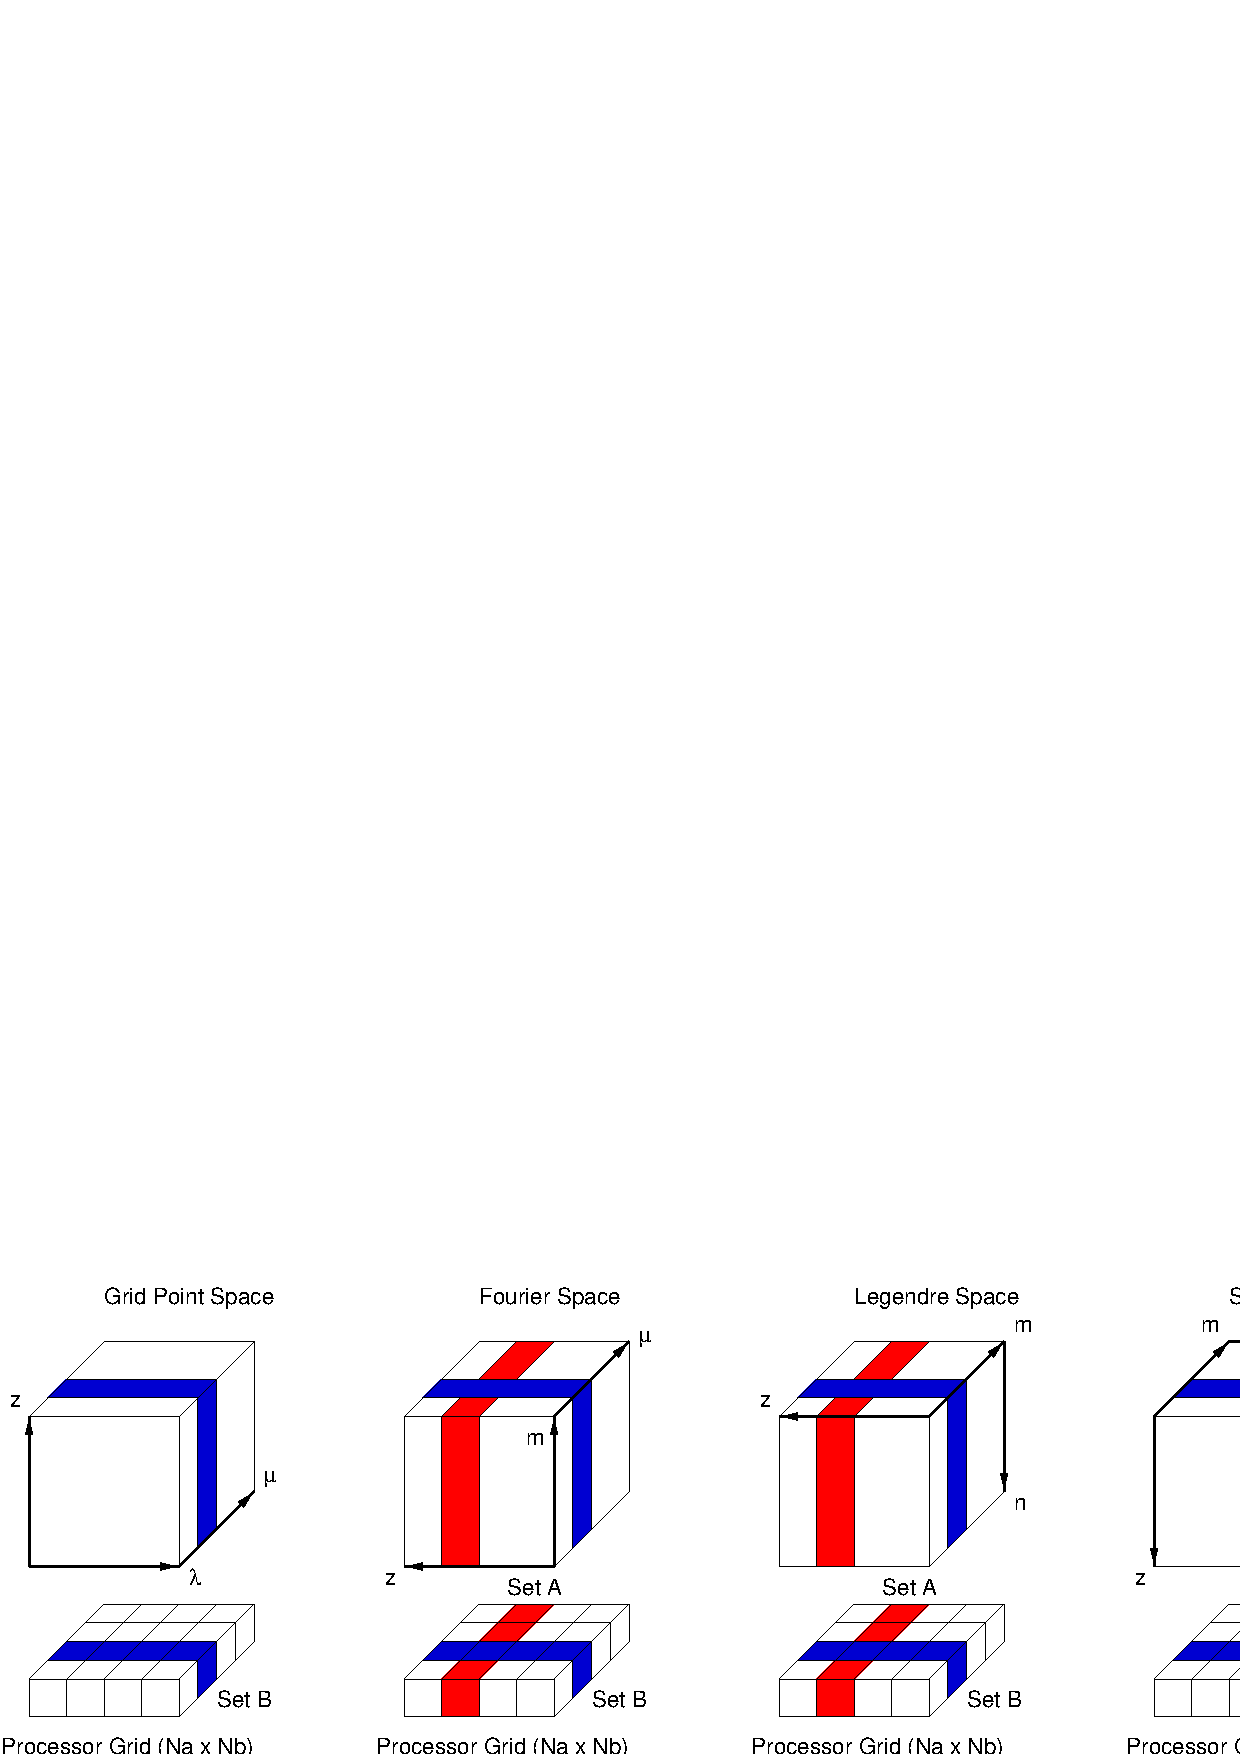
\includegraphics[width=12cm]{guide/transpose.pdf}}
%\else
%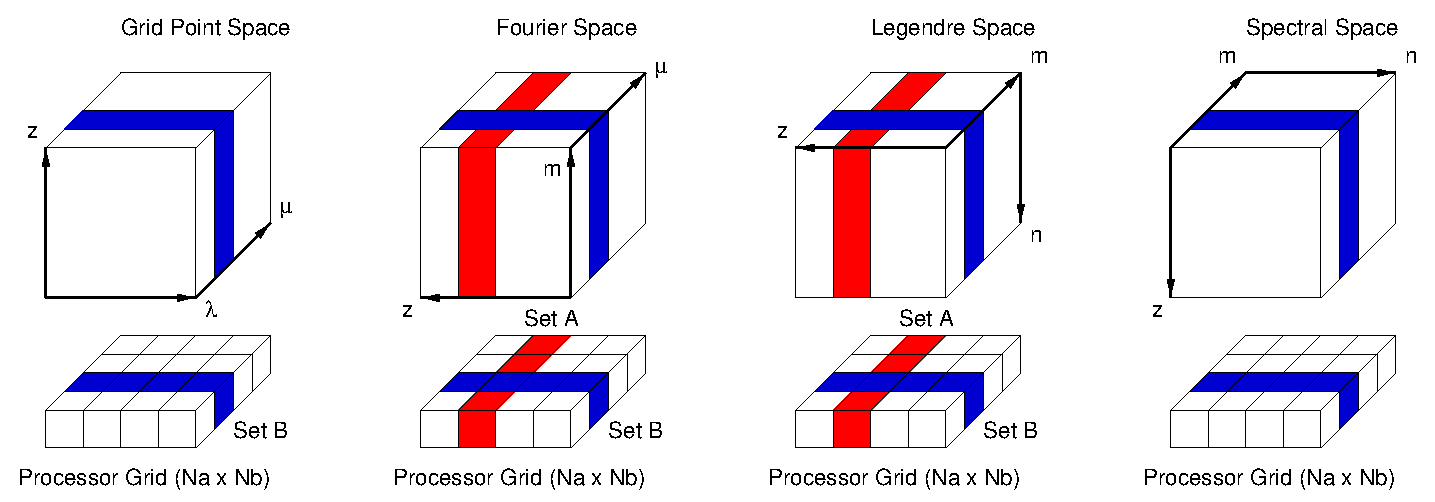
\includegraphics[width=12cm]{guide/transpose.eps}
%\fi
%\]
\caption{Data distribution}
\label{fig.transpose}
\end{figure}

The data transpositions, i.e. the redistribution of data in order to
perform the global Fourier and Legendre transformations are performed
just before and after these transformations. All other calculations
require almost no further communication (besides a few global sums)
because the data required for the operations is present on the
respective processor.  A recipe for writing parallel routines is given
in Section {\ref{sec.recipe}}.


\subsection{Recipe for writing or modifying parallel routines}
\label{sec.recipe}

\subsubsection{Physical parameterizations}

The physical parameterization routines (called from the routines {\tt
gpc} or {\tt physc}) work only on one block of grid cells of
consecutive longitudes. This block can be too short to accomodate all
grid cells of one latitude of it may combine grid cells of more than
one latitude into one block. The length of the block can be chosen
arbitrarily and is called {\tt nproma}. The loop
over the blocks is performed in a higher level routine ({\tt scan1})
and the actual block length 
is passed to the respective subroutines as {\tt kproma}.

``Physics'' computations at different model columns are generally
independent from 
each other and do not require any communication between
processors. Furthermore most computations do not depend on the
absolute location on the globe. If these two conditions are fullfilled
no further action is required for the parallel model version and a
physical parameterization routine may remain unchanged. Loops over the
grid cells in one block are performed by the following statement:
\begin{verbatim}
DO i=1, kproma
  ...
END DO
\end{verbatim}
Special care must be taken if:
\begin{enumerate}
\item The routines are not called within the loop over blocks.

In this case the number of longitudes and latitudes handled by the
processor can be accessed by reference to the components {\tt nglon}
and {\tt nglat} of the variable {\tt local\_decomposition} in module
{\tt mo\_decompose} (cf.{} Section {\ref{sec.decompose.grid}}). A
typical loop over blocks and block elements is given below.  {\tt
dc\%ngpblks} and {\tt dc\%nproma} ({\tt dc\%npromz}) are also used to
specify the 
dimensions of local arrays.
\begin{verbatim}
use mo_decomposition, only: dc => local_decomposition
real(dp) :: xlocal (dc%nproma, dc%ngpblks) ! declare a local array
...
DO j=1, dc%ngpblks-1                  ! loop over local block
  DO i=1, dc%nproma                   ! loop over grid cells in block
    ...
    xlocal (i,j) = 0._dp              ! access a local array
    ...
  END DO
END DO
DO i=1, dc%npromz
   ...
   xlocal (i,dc%ngpblks) = 0._dp
   ...
END DO
\end{verbatim}

\item An index to a global field is required or the absolute position on the
globe must be known.

These conditions are met in the short-wave radiation part, where the
zenith angle of the sun must be calculated, or if the horizontal area
covered by a column must be known, for instance in budget
calculations.

Every processor handles two distinct parts of the domain on opposite
sides of the globe. For this reason the first {\tt dc\%ngpblks/2}
blocks are located on the northern hemisphere whereas the
remaining lines are located on the southern hemisphere.
The local as well as the global
latitude generally runs from North to South, but some of the global
arrays (for instance Gaussian weights) are still stored in so called
ping-pong order (with one latitude line in the northern hemisphere
being followed by the respective latitude line from the southern
hemisphere).

For routines called within {\tt gpc} or {\tt physc} the local latitude
index {\tt jglat} and the global ping-pong index {\tt igprow} are
stored in the module variable {\tt nrow(2)} in module {\tt mo\_control}:
\begin{verbatim}
nrow(1) = igprow ! global ping pong index
nrow(2) = jlat   ! local  index north -> south
\end{verbatim}

\item Global sums are required.

Global sums should be avoided, in order to prevent communication
between processors. In the case that global operations cannot be
avoided, routines to derive global (or zonal) sums may be found in
module {\tt mo\_global\_op} (cf.{} Section\,{\ref{sec.globalop}}).

\item Dependencies between horizontal gridpoints exist.

Dependencies between horizontal gridpoints within the physical
routines should be avoided, in order to prevent communication between
processors. If possible these calculations should be done at locations
in the program where suitable data transpositions have already been
performed or in dedicated routines (for instance in the
semi--Lagrangian transport routine).

\item Input and Output

Input and Output is addressed in Section {\ref{sec.recipe.io}}

\end{enumerate}

\subsubsection{Input/Output}
\label{sec.recipe.io}

Two things must be considered when files are read or written:
\begin{enumerate}
\item 
  In parallel mode, only one processor is allowed to perform I/O. This
  processor will also be called I/O processor.
  The logical variable {\tt p\_parallel\_io} (from {\tt mo\_mpi}) has
  the value {\tt .true.} on the I/O processor only and has the value
  {\tt .false.} on all other processors.
  In single processor mode
  (indicated by a value {\tt .false.} of {\tt p\_parallel}) the data
  is merely read or written.
\item
  The values of variables read by the I/O processor must be communicated to the
  other processors. If all processors are supposed to receive the same
  information the broadcast routine {\tt p\_bcast} (from {\tt
  mo\_mpi}) must be called. In case of two or three dimensional arrays
  each processor only holds the information relevant for its
  subdomain. In this case the I/O must be performed on a global
  variable (generally only allocated on the processor which performs
  I/O) different from the local variable which finally is used for
  computations.  In order to communicate the data to processors in
  gridpoint space the routine {\tt scatter\_gp} from module {\tt
  mo\_transpose} must be called. Similar routines exist in order to
  distribute data in spectral space ({\tt scatter\_sp}) or do gather
  the data from the other processors ({\tt gather\_gp}, {\tt
  gather\_sp}). Generic interfaces are provided for the broadcast
  and gather or scatter routines
  (cf.{} Section\,{\ref{sec.mo-transpose}}) for different data types
  and array dimensions.
\end{enumerate}

Below some examples are given. Note that generally I/O is not
performed directly, but routines are provided for reading and writing
specific formats (Grib, Netcdf).

\begin{enumerate}
\item Read and broadcast some information

The broadcast routine requires {\tt p\_io} as actual parameter in
order to identify the processor which sends the information, i.e.{}
the processor which performs I/O.
\begin{verbatim}
  USE mo_mpi, ONLY: p_parallel, p_parallel_io, p_broadcast, p_io
  IF (p_parallel) THEN
     IF (p_parallel_io) THEN
        READ x
     ENDIF
     CALL p_bcast (x, p_io)
  ELSE
     READ x
  ENDIF
\end{verbatim}
\item Read and scatter some information

In this example {\tt x} is a 3 dimensional field
({\tt kbdim}, {\tt levels}, {\tt ngpblks}, where {\tt kbdim} is the
maximum length of block) which finally stores the local information
on each processor. Information on the data distribution of all
processors is provided in the variable {\tt global\_decomposition} and
must be passed to the scatter and gather routines.
\begin{verbatim}
  USE mo_mpi,       ONLY: p_parallel, p_parallel_io, p_io
  USE mo_transpose, ONLY: scatter_gp
  USE mo_decompose, ONLY: gl_dc => global_decomposition, &
                          dc    => local_decomposition
  REAL, POINTER :: tmp (:,:,:)                ! global read buffer
  REAL          :: x   (dc%nproma, dc%nlev, dc%ngpblks) 
  IF (p_parallel) THEN                        ! in parallel mode:
    NULLIFY(tmp)                       ! nullify global array not used
    IF(p_parallel_io) THEN
      ALLOCATE (tmp(dc%nlon,dc%nlev,dc%nlat)) ! allocate global array used
      READ x                                  ! read information
    ENDIF
    CALL scatter_gp(tmp, x, gl_dc)            ! scatter 
    IF (p_parallel_io) DEALLOCATE (tmp)       ! deallocate global array
  ELSE                                        ! in single processor mode:
     READ x                                   ! merely read  
  ENDIF
\end{verbatim}
\item Gather and write some information

This example is very similar to the previous one.
\begin{verbatim}
  USE mo_mpi,       ONLY: p_parallel, p_parallel_io, p_io
  USE mo_transpose, ONLY: gather_gp
  USE mo_decompose, ONLY: gl_dc => global_decomposition, &
                          dc    => local_decomposition
  REAL, POINTER :: tmp (:,:,:)                ! global read buffer
  REAL          :: x   (dc% nglon, dc% nlev, dc% nglat) 
  IF (p_parallel) THEN                        ! in parallel mode:
    NULLIFY(tmp)                       ! nullify global array not used
    IF(p_parallel_io) THEN
      ALLOCATE (tmp(dc%nproma,dc%nlev,dc%ngpblks)) ! allocate 
                                       !global array used
    ENDIF
    CALL gather_gp(tmp, x, gl_dc)             ! gather 
    IF(p_parallel_io) THEN
      WRITE x                                 ! write information
      DEALLOCATE (tmp)                        ! deallocate global array
    ENDIF
  ELSE                                        ! in single processor mode:
     WRITE x                                  ! merely write
  ENDIF
\end{verbatim}
\end{enumerate}

%\subsection{Message Passing Interface (mo\_mpi)}
% to be added in a later version

\subsection{Decomposition (mo\_decompose)}
\label{sec.decompose}

The decomposition is handled by the module {\tt mo\_decompose} which
is described in this section.

The domain decomposition is performed by a call to the routine {\tt
decompose} with the following parameters:

\begin{description}
\item{\tt global\_dc}\\
  Derived decomposition table (output).
\item{\tt nlat, nlon, nlev}\\
  These parameters determine the size of the global domain: {\tt nlat}
  is the number of latitudes (which must be even), {\tt nlon} is the
  number of longitudes and {\tt nlev} is the number of levels.
\item{\tt nm, nn, nk}\\
  These parameters give the number of wavenumbers in spectral
  space. Currently only triangular truncation is allowed with {\tt
  nm = nn = nk}.
\item{\tt nproca, nprocb}\\
  Following the ideas of the Integrated Forecast System (IFS) of the
  European Centre of Midium--Range Weather Forcast (ECMWF) the
  total domain is covered by {\tt nproca} times {\tt nprocb}
  processors. In Gridpoint space the domain is divided into {\tt
  nprocb} subdomains in east-west direction and 2 times {\tt nproca}
  subdomains in north-south directions. Details are given below in the
  subsections of this paragraph.

  The default decomposition may be modified by the following optional
  parameters:
\item{\tt norot}\\
  In order to improve load balancing in the shortwave radiation part
  half of the gridpoints of each processor should be exposed to the
  sun whereas the other half should be located at the nocturnal side
  of the globe. Thus each processor handles two subdomains on opposite
  sides of the globe. Actually the two domains must consist of
  latitude rows with the same absolute values of latitudes, but with
  opposite sign. The longitude values in the southern domain are
  rotated by 180 degree with respect to the corresponding gridpoints
  in the northern domain.
  Setting this optional parameter to {\tt .true.} the southern domain is
  not rotated. If the code runs on one processor this results in a
  continuous global domain as in the serial program version.
\item{\tt lfull\_m}\\
  Setting this optional parameter to {\tt .true.} ensures that the
  decomposition in spectral space does not spread wavenumbers with the
  same longitudinal wavenumber $m$ over different processors. This
  option is not recommended because it decreases load balance in
  spectral space.
\item{\tt debug}\\
  Setting this optional parameter to {\tt .true.} runs a second
  copy
  of the model using one additional processor so that ${\tt
  nproca}\times{\tt nprocb}+1$ processors are required in this
  case. Furthermore it is assumed that {\tt norot=.true.} for this
  additional run so that the decomposition corresponds with that of
  the original serial version.

  The values of the variables of the two model copies are compared
  at certain breakpoints and further tests for equality of
  corresponding variables can be inserted at any time of program
  execution. This is the most rigorous test of the parallel version.

  A value {\tt .true.} of the logical module variable {\tt
  debug\_parallel} indicates that the parallel test mode is enabled.
\end{description}

Decomposition information is stored in the module variables 
{\tt global\_decomposition} and {\tt local\_decomposition} of derived
type {\tt pe\_decomposed}. The elements of the array {\tt
global\_decomposition} describe the decomposition for each processor.
The scalar type {\tt local\_decomposition} holds the decomposition of
the actual processor.

The data type {\tt pe\_decomposed} described in the subsection below
holds the decomposition information for a single processor.

\subsubsection{Information on the whole model domain}

The following components of data type {\tt pe\_decomposed} have the
same contents for all processors of the model:

\begin{description}
\item{\tt nlon}: number of longitudes of the global domain.
\item{\tt nlat}: number of latitudes of the global domain.
\item{\tt nlev}: number of levels of the global domain.
\item{\tt nm}:   
maximum wavenumber used. Only triangular truncation is supported.

The following components depend on {\tt nm}:
\item{\tt nnp(m+1)}: 
number of spectral coefficients for each longitudinal wavenumber $m$,
$m=0,nm$
\item{\tt nmp(m+1)}:
displacement of the first point of m-columns within the array storing
the spectral coefficients. Actually {\tt nmp(1)=0} and {\tt
nmp(nm+2)=} last index of the array storing the spectral
coefficients. The actual number of coefficiens is $2\times nmp(nm+2)$
because 2 coefficients are stored for each wavenumber.
\end{description}

\subsubsection{Information valid for all processes of a model instance}
\label{sec.decompose.grid}

The following components of data type {\tt pe\_decomposed} have the
same contents for all processors of each instance of the model:

\begin{description}
\item{\tt nprocb}:
number of processors for the dimension that counts longitudes
\item{\tt nproca}:
number of processors for the dimension that counts latitudes
\item{\tt d\_nprocs}:
number of processors used in the model domain $nproca\times nprocb$.
\item{\tt spe, epe}:
Index number of first and last processor which handles this model domain.
\item{\tt mapmesh(ib,ia)}:
array mapping from a logical 2-d mesh to the processor index numbers
within the decomposition table {\tt global\_decomposition}. $ib=1,nprocb$;
$ia=1,nproca$.
\end{description}

\subsubsection{General Local Information}

The contents of the remaining components of data type {\tt
pe\_decomposed} is specific for each processor.

\begin{description}
\item{\tt pe}:
processor identifier. This number is used in the {\tt mpi} send and
receive routines.
\item{\tt set\_b}:
index of processor in the direction of logitudes. This number
determines the location within the array {\tt mapmesh}. processors
with ascending numbers handle subdomains with increasing longitudes
(i.e. from west to east).
\item{\tt set\_a}:
index of processor in the direction of latitudes. This number
determines the location within the array {\tt mapmesh}. Processors
with ascending numbers handle subdomains with decreasing values of
absolute latitudes (i.e. from the pole to the equator within each
hemisphere).
\end{description}

\subsubsection{Grid space decomposition}

In grid space longitudes and latitudes are spread over
processors. Each processor handles all levels of a model column.

\begin{description}
\item{\tt nglat, nglon}:
number of latitudes and longitudes in grid space handled by this processor.
\item{\tt glats(1:2), glate(1:2)}:
start and end values of global latitude indices. 
\item{\tt glons(1:2), glone(1:2)}:
start and end values of global of longitude indices.  Each processor
handles two subdomains located on opposite sides of the globe. The
first elements {\tt 1:nglat/2} of array dimensions indexing latitudes
correspond to global latitude indices {\tt glats(1):glate(1)}.  The
last elements {\tt nglat/2+1:nglat} correspond to global latitude
indices {\tt glats(2):glate(2)}.  Both, local and global latitude
indices run from north to south.  Elements
$e(i,j),i=1:nglon,j=1:nglat/2$ of a local array correspond to elements
$g(k,l),k=glons(1), glone(1),l=glats(1):glate(1)$ of the respective
global array.
\item{\tt glat(1:nglat)}:
global latitude index.
\item{\tt glon(1:nglon)}:
offset to global longitude index.  These components facilitate
indexing of global arrays. Elements $e(i,j),i=1:nglon,j=1:nglat/2$ of
a local array correspond to elements $g(glat(i),+glon(i)+j)$ of the
respective global array.
\end{description}

\subsubsection{Fourier space decomposition}

In order to perform the Fourier transformation, the arrays are
redistributed so that each processor holds all longitudes or Fourier
components. Latitudes are spread over processors as in grid
space. Additionally the levels are distributed.

\begin{description}
\item{\tt nflat, nflev}:
number of latitudes and levels on this processor.
\item{\tt nflevp1}:
number of levels plus one on this processor. If global arrays hold
{\tt nlev+1} elements per column they require {\tt nflevp1} on this
processor. {\tt nflevp1} is equal to {\tt nflev+1} if the last level
is handled by this processor, otherwise {\tt nflevp1} is equal to {\tt
nflev}.
\item{\tt flats(2), flate(2)}:
start and end values of latitudes indices. As in grid space 2
subdomains located on the northern and southern hemisphere are
handled.
\item{\tt flevs, fleve}:
start and end values of levels. The elements $e(k),k=1,nflevp1$ of a
local array correspond to elements $g(l),l=flevs:fleve$ of the
respective global array.
\item{\tt lfused}:
{\tt .true.} if this processor is used in Fourier space.
\end{description}

\subsubsection{Legendre space decomposition}

In order to perform the Legendre transformation, the arrays are
redistributed so that each processor holds all latitudes or spectral
coefficients for a given longitudinal wavenumber. Levels are spread
over processors as in Fourier space. Additionally the longitudinal
wavenumbers are distributed.

Row of PEs with same set\_a:
\begin{description}
\item{\tt nlm}:
number of local longitudinal wave numbers m handled by this processor.
\item{\tt lm(1:nlm)}:
actual longitudinal wave numbers handled by this processor.
\item{\tt lnsp}:
number of complex spectral coefficients handled by this processor.
\item{\tt nlmp(1:nlm)}:
displacement of the first coefficient of columns (with same
longitudinal wave number) within a globally indexed array (as described
by components {\tt nm}, {\tt nnp}, {\tt nmp}).
\item{nlnp(1:nlm)}:
number of points on each column with same longitudinal wave number m.
\item{nlnm0}:
number of coefficients with longitudinal wave number m=0 on this processor.
\end{description}

Column of PEs with same set\_b:
\begin{description}
\item{\tt nllev, nllevp1}:
number of levels (+1) handled by this processor as in Fourier space.
\item{\tt llevs, lleve}:
start and end values of level indices as in Fourier space.
\end{description}

\subsubsection{Spectral space decomposition}

For spectral computations the arrays are redistributed so that each
processor holds all levels for a given spectral
coefficient. Longitudinal wavenumbers are spread over processors as in
Legendre space. Remaining spectral coefficients are spread over
processors.

\begin{description}
\item{\tt snsp, snsp2}:
number of spectral coefficients handled by this processor and number
of coefficients multiplied by 2.
\item{\tt ssps, sspe}:
first and last spectral coefficient with respect to the ordering in
Legendre space.
\item{\tt lfirstc}:
true, if first global coefficient (m=0,n=0) resides on this processor.
\item{\tt ifirstc}:
location of first global coefficient on this processor.
\item{\tt np1(1:snsp)}:
value of (n+1) for all coefficients of this processor.
\item{\tt mymsp(1:snsp)}:
value of m for all coefficients of this processor.
\item{\tt nns}:
number of different n-values for this processor.
\item{\tt nindex(1:nns)}:
values of (n+1) different n-values for this processor.
\item{\tt nsm}:
number of longitudinal wavenumbers per processor.
\item{\tt sm (1:nsm)}:
actual longitudinal wave numbers handled by this processor.
\item{\tt snnp(1:nsm)}:
number of n coefficients per longitudinal wave number m.
\item{\tt snn0(1:nsm)}:
first coefficient n for a given m.
\item{\tt nsnm0}:
number of coefficients with m=0 on this processor.
\end{description}

\subsection{Gather, Scatter and Low Level Transposition Routines 
(mo\_transpose)}
\label{sec.mo-transpose}

The module {\tt mo\_transpose} holds the routines to scatter global
fields (after input) among the processors, to gather distributed
fields from the processors (for output and debug purposes) and to
perform the transpositions between the different decompositions (grid,
Fourier, Legendre and spectral space). 

\subsubsection{Gather and Scatter routines (gather\_xx, scatter\_xx)}

Generic interfaces are defined for specific routines to act on arrays
of different rank (for 3-D atmospheric fields, 2-D surface fields,
etc.\ ). Arrays of rank 4 are supported in order to handle arrays
allocated in memory buffer. The actual representation (2-D, 3-D) is
derived from the shape of the rank 4 arrays or rank 3 arrays.

All scatter and gather routines have a similar interface:

\begin{description}
\item{\tt subroutine scatter\_xx (gl, lc, gl\_dc)}
\item{\tt subroutine gather\_xx (gl, lc, gl\_dc, [source])}
\end{description}

The postfix {\tt xx} is one of {\tt gp}, {\tt ls}, {\tt sa} or {\tt
sp} and denotes the space to scatter/gather to/from.

The parameter {\tt gl} is a pointer of rank 1 to 4 pointing to the
global array. {\tt gl} needs to be allocated only on the processor
which performs i/o.

The parameter {\tt lc} is an array of the same rank as {\tt gl}
holding the distributed array.

The parameter {\tt gl\_dc} holds the global decomposition table.

All scatter routines distribute a global array from the i/o processor
to the decomposed arrays of all processors, including itself.

The gather routines have an optional parameter {\tt source} in order
to gather fields from different model copies run in parallel for
debug purposes. {\tt source} may have one of the following values:
\begin{description}
\item{\tt -1:} 
gather from all processors. If more than one model copy is run,
the result depends on the actual I/O processor within the
global decomposition table.
\item{\tt 0:}
gather from the i/o processor only. If more than one model copy is
run this is the processor which performs calculations on the whole
model domain.
\item{\tt 1:}
gather from all processors besides the I/O processor. If more than one
model copy is run these processors perform the parallel
calculations on the distributed domain.
\item{\tt not present:} 
The effect is the same as if {\tt source} had the value of the
variable {\tt debug\_parallel} in {\tt mo\_decompose}.
\end{description}

The shape of the arrays {\tt gl} may be one of the following:

\begin{description}
\item{\tt scatter\_gp, gather\_gp}: (grid space)

\begin{tabular}{llll|l}
(nlon,&nlev,&ntrac,&nlat)&3D tracer fields\\
\hline
(nlon,&nlev,&nlat,&1)    &3D gridpoint field\\
(nlon,&nlev,&nlat)&      &\\
\hline
(nlon,&nlat,&1,&1)       &2D surface field\\
(nlon,&nlat,&1)&&\\
(nlon,&nlat)&&&\\
\end{tabular}

{\tt nlon}, {\tt nlat} are the number of longitudes and latitudes of
the global field {\tt gl} as specified by the respective components of
{\tt local\_decomposition}. {\tt nlev}, {\tt ntrac} are arbitrary
numbers of vertical 
levels and tracers.  {\it If more longitudes are passed only {\tt
nlon} or {\tt nglon} longitudes are scattered/gathered.}

\item{\tt scatter\_sp, gather\_sp}: (spectral space)

\begin{tabular}{llll|l}
(nlev,&2,&nsp,&1)& full spectral field\\
(nlev,&2,&nsp)&  & \\
\hline
(nlev,&nnp1,&1,&1)& spectral array with \\
(nlev,&nnp1,&1)&  & m=0 coefficients only \\
(nlev,&nnp1)&  &  & (zonal mean in grid space) \\
\end{tabular}

The global field {\tt gl} has {\tt nsp} spectral coefficients or {\tt
nnp1} coefficients for the zonal wavenumber m=0 only as specified by
the respective components of {\tt local\_decomposition}.  The
corresponding decomposed field {\tt lc} has {\tt snsp} spectral
coefficients or {\tt nsnm0} coefficients for the zonal wavenumber m=0
only.  {\tt nlev} is an arbitrary number of vertical levels.  The
second index is 2 because 2 coefficients are stored for each
wavenumber.

\item{\tt scatter\_sa, gather\_sa}: (symmetric/assymetric Fourier components)

\begin{tabular}{llll|l}
(nlev,&2,&nm+1,&nhgl)& full Fourier transformed field\\
\hline
(nlev,&nhgl,&1,&1)& Fourier transformed field (m=0 only)\\
(nlev,&nhgl)&  &  & (zonal mean in grid space)\\
\end{tabular}

For reasons of computational efficiency, Legendre transformation is
performed on symmetric and asymmetric (with respect to the equator)
fields seperately. The symmetric/asymmetric Fourier components are
input to the Legendre transform (output of the inverse
transform). Thus, the decomposition of these fields corresponds to
Legendre space, i.e.\ vertical levels and zonal wavenumbers are spread
over processors.

The global field {\tt gl} has {\tt nm+1} zonal wavenumbers and {\tt
nlev} or {\tt nlev+1} vertical levels as specified by the respective
components of {\tt local\_decomposition}.  The corresponding
decomposed field {\tt lc} has {\tt nlm} zonal wavenumbers and {\tt
nllev} or {\tt nllevp1} vertical levels. {\tt nhgl=nlat/2} is half of the
number of Gaussian latitudes. The second index of the full fields is 2
because 2 coefficients are stored for each wavenumber.

\item{\tt scatter\_ls, gather\_ls}: (Legendre space)

Scatter and gather routines to/from Legendre space are used for
debugging purposes only. 

\begin{tabular}{llll|l}
(2*(nm+1),&nlev,&nlat,&nvar)& Fourier components, (gather routine
only)\\
\hline
(nlev,&2,&nsp)&& full spectral field\\
\hline
(nlev,&nnp1)&&& spectral field with m=0 only\\
\end{tabular}

Global Fourier transformed fields (in Legendre space distribution)
have {\tt 2*(nm+1)} spectral coefficients and {\tt nlev} or {\tt
nlev+1} vertical levels as specified by the respective components of
{\tt local\_decomposition}. Global spectral fields have {\tt nsp}
spectral wavenumbers or {\tt nnp1} coefficients for m=0 only. The
corresponding decomposed field {\tt lc} has {\tt nlm} zonal
wavenumbers or {\tt lnsp} complex spectral coefficients and {\tt
nllev} or {\tt nllevp1} vertical levels. {\tt nlat} is the number of
latitudes and {\tt nvar} an arbitrary number of variables.

\end{description}

\subsubsection{Transposition routines (tr\_xx\_yy)}

The general interface of the transpose routines is:

{\tt subroutine tr\_xx\_yy (gl\_dc, sign, xxfields.., yyfields..)}\\
{\tt\quad TYPE (pe\_decomposed) :: gl\_dc}\quad decomposition table\\
{\tt\quad INTEGER :: sign}\quad direction of transposition:  
1: xx$-\!\!\!>$yy, -1: xx$<\!\!\!-$yy\\
{\tt\quad REAL :: xxfields}\quad fields in $xx$-space\\
{\tt\quad REAL :: yyfields}\quad fields in $yy$-space

With $xx$, $yy$ being one of {\tt gp} (gridpoint space), {\tt ls}
(Legendre space), or {\tt sp} (spectral space).  The shape of the
array arguments {\tt xxfields}, {\tt yyfields} depends on the data
structure in the respective spaces. The specific interfaces are as
follows:

\begin{verbatim}
SUBROUTINE tr_gp_fs (gl_dc, sign, gp1, gp2, gp3, gp4, gp5, gp6, gp7,&
                     sf1, sf2, sf3, zm1, zm2, zm3, fs, fs0)
!
! transpose
!   sign= 1 : grid point space  -> Fourier space
!   sign=-1 : grid point space <-  Fourier space
! 
!
TYPE (pe_decomposed) ,INTENT(in)     :: gl_dc  (:)       ! decomposition
INTEGER              ,INTENT(in)     :: sign             ! 1:gp>fs; -1:gp<fs
REAL                 ,INTENT(inout)  :: gp1    (:,:,:)   ! gridpoint space 3d
                                        ...
REAL                 ,INTENT(inout)  :: gp7    (:,:,:)   ! 
REAL ,OPTIONAL       ,INTENT(inout)  :: sf1    (:,:)     ! gridpoint space 2d
REAL ,OPTIONAL       ,INTENT(inout)  :: sf2    (:,:)     ! gridpoint space 2d
REAL ,OPTIONAL       ,INTENT(inout)  :: sf3    (:,:)     ! gridpoint space 2d
REAL ,OPTIONAL       ,INTENT(inout)  :: zm1    (:,:)     ! zonal mean
REAL ,OPTIONAL       ,INTENT(inout)  :: zm2    (:,:)     ! zonal mean
REAL ,OPTIONAL       ,INTENT(inout)  :: zm3    (:,:)     ! zonal mean
REAL                 ,INTENT(inout)  :: fs     (:,:,:,:) ! Fourier space
REAL ,OPTIONAL       ,INTENT(inout)  :: fs0    (:,:,:)   ! zonal mean, Four.
\end{verbatim}

\begin{verbatim}
SUBROUTINE tr_fs_ls (gl_dc, sign, fs, ls, fs0, ls0)
!
! transpose
!   sign= 1 : Fourier space  -> Legendre space
!   sign=-1 : Fourier space <-  Legendre space
!
TYPE (pe_decomposed) ,INTENT(in)     :: gl_dc  (:)       ! decomposition
INTEGER              ,INTENT(in)     :: sign             ! 1:fs>ls; -1:gs<ls
REAL                 ,INTENT(inout)  :: fs   (:,:,:,:)   ! fs
REAL                 ,INTENT(inout)  :: ls   (:,:,:,:)   ! ls
REAL ,OPTIONAL       ,INTENT(inout)  :: fs0  (:,:,:)     ! fs, zonal means
REAL ,OPTIONAL       ,INTENT(inout)  :: ls0  (:,:,:)     ! ls, zonal means
\end{verbatim}

\begin{verbatim}
SUBROUTINE tr_ls_sp (gl_dc, sign, ls1, sp1, ls2, sp2, ls3, sp3, ls0, sp0)
!
! transpose
!   sign= 1 : Legendre space  -> spectral space
!   sign=-1 : Legendre space <-  spectral space
!
TYPE (pe_decomposed) ,INTENT(in)     :: gl_dc (:)     ! decomposition
INTEGER              ,INTENT(in)     :: sign          ! 1:ls&gtsp; -1:ls&ltsp
REAL                 ,INTENT(inout)  :: ls1   (:,:,:) ! Legendre space 
REAL                 ,INTENT(inout)  :: sp1   (:,:,:) ! spectral space
                                        ...
REAL                 ,INTENT(inout)  :: ls3   (:,:,:) ! Legendre space
REAL                 ,INTENT(inout)  :: sp3   (:,:,:) ! spectral space
REAL ,OPTIONAL       ,INTENT(inout)  :: ls0   (:,:)   ! Legendre (m=0 only)
REAL ,OPTIONAL       ,INTENT(inout)  :: sp0   (:,:)   ! spectral (m=0 only)
\end{verbatim}

\subsection{High Level Transposition Routines (mo\_call\_trans)}
\label{sec.mo_call_trans}

The routines in module {\tt mo\_call\_trans} gather the fields to be
transposed from the respective modules and pass them as actual
parameters to the routines which finally perform the transformations
(defined in module {\tt mo\_transpose}). 
If ECHAM is run in test mode, the
correctness of the parallel implementation is tested by calling the
respective routines for the ingoing and outgoing parameters.
Test routines are also provided for the content of some buffers.

The fields involved in the
transformation and test routines are listed below.

\begin{center}
\begin{tabular}{|ll|}
\hline
subroutine & spectral\_to\_legendre \\
\hline
Input : & from module mo\_memory\_ls (Legendre space) \\
ld & \\
ltp & \\
lvo & \\
lu0 & \\
\hline
Output :& to module mo\_memory\_sp (spectral space) \\
sd & \\
stp & \\
svo & \\
su0 & \\
\hline
\end{tabular}

\begin{tabular}{|ll|}
\hline
subroutine & legendre\_to\_fourier\\ \hline
Input : & from module mo\_buffer\_fft (Legendre space)\\
fftl & buffer for 2D and 3D fields \\
lbm0 & buffer for zonal means (m=0) \\
\hline
Output :& to module mo\_buffer\_fft (Fourier space)\\
fftz & buffer for 2D and 3D fields \\
fbm0 & buffer for zonal means (m=0) \\
\hline
\end{tabular}

\begin{tabular}{|ll|}
\hline
subroutine & fourier\_to\_gridpoint\\ \hline
Input : & from module mo\_buffer\_fft (Fourier space)\\
fftz & buffer for 2D and 3D fields \\
fbm0 & buffer for zonal means (m=0) \\
\hline
Output :& to module mo\_scan\_buffer (gridpoint space)\\
d\_scb & \\
t\_scb & \\
u\_scb & \\
v\_scb & \\
vo\_scb & \\
dtm\_scb & \\
dtl\_scb & \\
alps\_scb & \\
dalpsl\_scb & \\
dalpsm\_scb & \\
u0\_scb & \\
du0\_scb & \\
ul\_scb & \\
\hline
\end{tabular}

\begin{tabular}{|ll|}
\hline
subroutine & gridpoint\_to\_fourier\\ \hline
Input : & from module mo\_scan\_buffer (gridpoint space)\\
rh\_scb & \\
dm\_scb & \\
vom\_scb & \\
vol\_scb & \\
u0\_scb & \\
du0\_scb & \\
ul\_scb & \\
\hline
Input : & from module mo\_memory\_g1a (gridpoint space)\\
alpsm1 & \\
dm1 & \\
tm1 & \\
vom1 & \\
\hline
Output :& to module mo\_buffer\_fft (Fourier space)\\
fftz & buffer for 2D and 3D fields \\
fbm0 & buffer for zonal means (m=0) \\
\hline
\end{tabular}

\begin{tabular}{|ll|}
\hline
subroutine & fourier\_to\_legendre\\ \hline
Input : & from module mo\_buffer\_fft (Fourier space)\\
fftz & buffer for 2D and 3D fields \\
fbm0 & buffer for zonal means (m=0) \\
\hline
Output :& to module mo\_buffer\_fft (Legendre space)\\
fftl & buffer for 2D and 3D fields \\
lbm0 & buffer for zonal means (m=0) \\
\hline
\end{tabular}

\begin{tabular}{|ll|}
\hline
subroutine & legendre\_to\_spectral\\ \hline
Input : & from module mo\_memory\_ls (Legendre space) \\
ld & \\
ltp & \\
lvo & \\
lu0  & \\
\hline
Output :& to module mo\_memory\_sp (spectral space) \\
sd & \\
stp & \\
svo & \\
su0 & \\
\hline
\end{tabular}

\begin{tabular}{|ll|}
\hline
subroutine & test\_memory\_f (text) \\ \hline
Test : & module mo\_memory\_f \\
f & \\
\hline
\end{tabular}

\begin{tabular}{|ll|}
\hline
subroutine & test\_memory\_gp (text)\\ \hline
\hline
\end{tabular}

\begin{tabular}{|ll|}
\hline
subroutine & test\_scan\_buffer (gp, text)\\ \hline
\hline
\end{tabular}

\begin{tabular}{|ll|}
\hline
subroutine & test\_row\_buffer (j, text)\\ \hline
& \\
\hline
\end{tabular}
\end{center}

%\subsection{Module containing subprograms for testing ({\tt mo\_test\_trans})

\subsection{Global operations ({\tt mo\_global\_op})}\label{sec.globalop}

In this module, subprograms are collected that perform global
operations on 2--d and 3--d fields like the calculation of global or
zonal mean values. Any global operation needs communication between
the processors. Even if integrals are split into integrals over the
domain that is present on each processor and the summation over all
processors, the global operation subroutines slow down the \echam{}
program the more the more processors are used in a simulation. For
this performance reason, it is highly recommended to reduce global
operations to a strict minimum in \echam{} and to perform such
operations in the postprocessing step that can be performed in
parallel to a longer simulation.

%\subsection{Semilagrangian transport}


  \section{Data structures and memory use}\label{secstreams}

     \subsection{Output Streams and Memory Buffer}
\label{sec.output_stream}
%------------------------------------------------------------------------------
\subsubsection{Functionality}

The {\bf Output Stream} interface maintains a list of output
streams. Generally one ore more streams are associated to an output
file. Each stream has attributes specifying the file name, file type,
etc.{}. It further holds a linked list of {\bf Memory Buffer elements},
of 2 to 4 dimensional arrays and associated meta information.

%------------------------------------------------------------------------------
\subsubsection{Usage}

First, a new output stream must be created by calling subroutine {\tt
new\_stream}\index{streams!new\_stream}. 
Afterwards fields may be allocated by calling {\tt
add\_stream\_element}\index{streams!add\_stream\_element}.

\subsubsection*{Create a new output stream}

The access to the output stream interface is provided by module {\tt
mo\_memory\_base}\index{streams!mo\_memory\_base}
\index{memory!mo\_memory\_base}:
%
{\small
\begin{verbatim}
  USE mo_memory_base, ONLY: t_stream,                                    &
                            new_stream, delete_stream,                   &
                            default_stream_setting, add_stream_element,  &
                            get_stream_element, set_stream_element_info, &
                            memory_info,                                 &
                            ABOVESUR2, ...
\end{verbatim}}
%
To create a new output stream the routine {\tt
new\_stream}\index{streams!new\_stream} has to be called:
%
{\small
\begin{verbatim}
  TYPE (t_stream) ,pointer :: mystream
  ...
  CALL new_stream (mystream ,'mystream')
\end{verbatim}}
%
{\tt mystream} is a pointer holding a reference to the output stream
returned by subroutine {\tt new\_stream}. {\tt 'mystream'} is the
identification name
of the output stream.

By default, the output and rerun filenames are derived from the name
of the output stream (here 'mystream') by appending a respective
suffix (here {\tt '\_mystream'}) to the standard filenames.  The
content of the output stream is written to the rerun file and to the
output file. To change the defaults, optional parameters may be provided
(cf.{} section \ref{sec.new_stream}).

\subsubsection*{Add a field to an output stream}

To include items in the output stream {\tt mystream} the routine {\tt
add\_stream\_element} has to be called. A unique name must be given to
identify the quantity and a pointer associated to the field is
returned. For example, to add a surface field {\tt a} and an
atmospheric field {\tt b} with names {\tt 'A'} and {\tt 'B'}, the
following sequence of subroutine calls is 
required\index{streams!add\_stream\_element}:
%
{\small
\begin{verbatim}
  REAL, POINTER :: a (:,:)
  REAL, POINTER :: b (:,:,:)
  REAL, POINTER :: c (:,:)
  ...
  CALL add_stream_element (mystream, 'A' ,a )
  CALL add_stream_element (mystream, 'B' ,b )
\end{verbatim}}
%
By default suitable sizes are assumed for surface (2-d pointer {\tt
a}) or atmospheric fields (3-d pointer {\tt b}).  To choose
other sizes (e.g.{} spectral fields or a non-standard number of
vertical layers) optional parameters must be specified.  The
specification of the optional parameters is given in section
{\ref{sec.add_stream_element}}

A routine is available to associate a pointer (here {\tt c}) with an
item (here {\tt 'A'}) already included in the list (previously by another
sub-model for example):
%
{\small
\begin{verbatim}
  CALL get_stream_element (mystream, 'A', c)
\end{verbatim}}
%
If stream element {\tt 'A'} has not been created beforehand, a null
pointer is returned for {\tt c}.

%------------------------------------------------------------------------------
\subsubsection{Create an output stream}
\label{sec.new_stream}

Optional parameters may be passed to subroutines
{\tt new\_stream} and {\tt add\_stream\_element}
in order to specify the attributes of output streams
and memory buffers. Furthermore, routines are available to
change default values for optional parameters.

The interface of the routine to create an output stream 
is\index{streams!new\_stream}:

{\small
\begin{tabular}{|llllp{7cm}|}
\hline
\multicolumn{2}{|l}
{\tt SUBROUTINE new\_stream}&
\multicolumn{3}{p{11cm}|}
                         {\tt (stream ,name [,filetype]
                         [,post\_suf] [,rest\_suf] [,init\_suf]
                         [,lpost] [,lpout] [,lrerun] [,lcontnorest] 
                         [,linit] [,interval])}\\
\hline
name&type&intent&default&description\\
\hline
\,stream     &type(t\_stream)&pointer&       & Returned reference to
                                               the new output stream.\\
\,name       &character(len=*) &in  &        & Name of the new output stream.\\
{[filetype]} &integer      &in      &out\_filetype & Type of output
                                               file. The default
                                               (GRIB) may be changed
                                               in namelist 
                                               /SDSCTL/. Alternatively 
                                               NETCDF may be passed.\\
{[post\_suf]}&character(len=*) &in      &'\_'//name& Suffix of the
                                               output file associated
                                               with the stream. The
                                               default is derived from
                                               the name of the output
                                               stream.\\
{[rest\_suf]}&character(len=*) &in      &'\_'//name& Suffix of the
                                               rerun file.\\
{[init\_suf]}&character(len=*) &in      &'\_'//name& Suffix of initial file.\\
{[lpost]}    &logical      &in      &.true.  & Postprocessing flag. If
                                               .true.{}
                                               an output file is
                                               created for this stream.\\
{[lpout]}    &logical      &in      &.true.  & Output flag. The stream
                                               is written to the
                                               output file if {\tt
                                                 lpout=.true} \\
{[lrerun]}   &logical      &in      &.true.  & If .true.{} the stream
                                               is read/written from/to the
                                               rerun file.\\
{[lcontnorest]} &logical   &in      &---     & Continue a restart even
if this stream is not present in any rerun file. \\
{[linit]}    &logical      &in      &.true.  & Write to initial file
(does not work?)\\
{[interval]}&type(io\_time\_event)&in&putdata& Postprocessing output
                                               interval. Default:
                                               12 hours.\\
\hline
\multicolumn{5}{p{16cm}}{Optional parameters are given in brackets [ ].
They should always be passed by keyword because the number and
ordering of optional parameters may change.}\\
\end{tabular}}

Valid values for the argument {\tt out\_filetype} are defined within
module {\tt mo\_memory\_base}\index{streams!mo\_memory\_base}:
{\small
\begin{verbatim}
  INTEGER ,PARAMETER :: GRIB      = 1
  INTEGER ,PARAMETER :: NETCDF    = 2
\end{verbatim}}

For specification of a non-standard output time interval data type
{\tt io\_time\_event}\index{data type!io\_time\_event} 
(defined in module {\tt mo\_time\_event}
\index{time manager!mo\_time\_event}) 
has to
be passed as argument {\tt interval}. For example, in order to write
every time step or in 6 hourly intervals, specify: {\tt
interval=io\_time\_event(1,'steps','first',0)} or {\tt
(6,'hours','first',0)}, respectively.

Once a stream has been created, a reference can be obtained by calling
subroutine {\bf get\_stream}\index{streams!get\_stream}:

{\small
\begin{tabular}{|llllp{7cm}|}
\hline
\multicolumn{5}{|l|}
{\tt SUBROUTINE get\_stream (stream ,name)}\\
\hline
name&type&intent&default&description\\
\hline
\,stream     &type(t\_stream)&pointer&       & Returned reference to the
                                               output stream.\\
\,name       &character(len=*) &in      &        & Name of the output stream.\\
\hline
\end{tabular}}


%------------------------------------------------------------------------------
\subsubsection{Add a field to the output stream}
\label{sec.add_stream_element}

The routine to add new elements to the output stream 
is\index{streams!add\_stream\_element}:

{\small
\begin{tabular}{|llllp{6cm}|}
\hline
\multicolumn{3}{|l}
{\tt SUBROUTINE add\_stream\_element}&
\multicolumn{2}{p{9cm}|}
 {\tt (stream ,name ,ptr [,ldims] [,gdims]
 [,klev] [,ktrac] [,units] [,longname] [,repr] 
 [,lpost] [,laccu] [lmiss,] [missval,] [,reset] [,lrerun] [,contnorest]
 [,table] [,code] [,bits] [,leveltype] 
 [,dimnames] [,mem\_info] [,p4] [,no\_default] [,verbose])}\\
\hline
name&type&intent&default&description\\
\hline
%------------------------------------------------------------------------------
\multicolumn{5}{|l|}{\bf mandatory arguments :}\\
stream     &type(t\_stream) &inout    &     & Output stream.\\
name       &character(len=*)&in       &     & Name of the field to add
                                              to the output stream.\\
ptr        &real(:,:[,:][,:])&pointer &     & Returned reference to
                                              the memory of the
                                              2- or 3- or 4-dimensional
                                              field.\\
\hline
%------------------------------------------------------------------------------
\multicolumn{5}{|l|}{\bf specification of dimensions :}\\
{[ldims(:)]}   &integer     &in &cf.\,text & Local size on actual processor.\\
{[gdims(:)]}   &integer     &in &cf.\,text & Global size of the
field.\\
{[klev]}       &integer     &in &cf.\,text & Number of vertical levels.\\
{[ktrac]}      &integer     &in &0         & Number of tracers. \\
{[repr]}       &integer     &in &GRIDPOINT & Representation.\\
{[leveltype]}  &integer     &in &cf.\,text & Dimension index of the
                                             vertical coordinate.\\
\hline
%------------------------------------------------------------------------------
\multicolumn{5}{|l|}{\bf postprocessing flags :}\\
{[lpost]}      &logical &in&.false.& Write the field to the
                                     postprocessing file.\\
{[laccu]}      &logical &in&.false.& ``Accumulation'' flag: Does no
accumulation but divides variable by the number of seconds of the
output interval and resets it to {\tt reset} after output.\\
{[reset]}      &real    &in&0.     & Reset field to this value at initialization,
and after output if {\tt laccu=.true.} or {\tt reset} is not zero.\\
\hline
%------------------------------------------------------------------------------
\multicolumn{5}{|l|}{\bf rerun flags :}\\
{[lrerun]}     &logical &in&.false.& Flag to read/write field from/to
                                     the rerun file.\\
{[contnorest]} &logical &in&.false.& If {\tt contnorest=.true.},
continue restart, stop otherwise.\\
\hline
%------------------------------------------------------------------------------
\multicolumn{5}{|l|}{\bf attributes for NetCDF output :}\\
{[units]}      &character(len=*)&in&' '                & Physical units.\\
{[longname]}   &character(len=*)&in&' '                & Long name.\\
{[dimnames(:)]}&character(len=*)&in&'lon'[,'lev'],'lat'& Dimension names.\\ 
\hline
%------------------------------------------------------------------------------
\multicolumn{5}{|l|}{\bf attributes for GRIB output :}\\
{[table]}      &integer     &in& 0  & table number.\\
{[code]}       &integer     &in& 0  & code number.\\
{[bits]}       &integer     &in& 16 & number of bits used for encoding.\\
\hline
%------------------------------------------------------------------------------
\multicolumn{5}{|l|}{\bf Missing values :} \\
{[lmiss]}      &logical     &in&.false.&If {\tt lmiss=.true.}, missing
values are set to {\tt missval}, not set at all otherwise.\\
{[missval]}    &real        &in& $-9\times10^{33}$& missing value.\\
%------------------------------------------------------------------------------
\multicolumn{5}{|l|}{\bf miscellaneous arguments :}\\
{[mem\_info]}  &type(memory\_info)&pointer&&Reference to meta data information.\\
{[p4(:,:,:,:)]}&real              &pointer&& Pointer to allocated memory provided.\\
{[no\_default]}&logical         &in&.false.&Default values usage flag.\\
{[verbose]}    &logical         &in&.false.&Produce diagnostic printout.\\ 
\hline
\end{tabular}}

Most arguments of the routine are optional. They may be given for the
following purposes:
\begin{description}
\item{\bf specification of dimensions:}\\
  The total size of the field is specified by the parameter {\tt
  gdims}. In a parallel environment, the part allocated on a processor
  element is specified by the parameter {\tt ldims}. The order of
  dimensions is (lon,lat) for 2--d, (lon,lev,lat) for 3--d and
  (lon,lev,any,lat) for 4--dimensional gridpoint fields. The number of
  size of {\tt gdims} and {\tt ldims} corresponds to the rank of {\tt
  ptr(:,:)}.

  Generally, it is not necessary to give dimension information. The
  sizes of the 
  fields are derived from the model field sizes.  If a 2--dimensional
  pointer {\tt ptr(:,:)} is provided for {\tt ptr}, a SURFACE field is
  assumed. If a 3-dimensional pointer {\tt ptr(:,:,:)} is provided, a
  HYBRID field (lon,lev,lat) is assumed.

  For the following cases optional arguments must be specified to
  overwrite the defaults:
  \begin{description}
  \item{\bf The number of vertical levels differs from the number of
  model levels}\\

    To specify a number of levels different from the standard
    $\sigma$--hybrid co--ordinate system used in the model, the
    parameter {\tt klev} 
    may be specified. A HYBRID coordinate system is assumed in this
    case. However if the field is written to the postprocessing file
    {\tt (lpost=.true.)}, it is recommended to either pass a dimension
    index to parameter {\tt leveltype} or the name of the dimensions
    to {\tt dimnames} in order to pass proper attributes to the
    NetCDF and GRIB writing routines.

    For the usual cases, dimension indices are predefined (cf.~table
    \ref{tab.dims}) and may be accessed from module {\tt mo\_netcdf}.
    New dimensions may be defined by the use of the subroutine {\tt
    add\_dim} as described in section \ref{sec.dim}.

  \item{\bf The field is not a gridpoint field}\\
    For non Gaussian gridpoint fields appropriate values should be
    passed as parameter {\tt repr}. Predefined values ({\tt
      mo\_linked\_list}) are:
  {\small
\begin{verbatim}
     INTEGER ,PARAMETER :: UNKNOWN   = -huge(0)
     INTEGER ,PARAMETER :: GAUSSIAN  = 1
     INTEGER ,PARAMETER :: FOURIER   = 2
     INTEGER ,PARAMETER :: SPECTRAL  = 3
     INTEGER ,PARAMETER :: HEXAGONAL = 4
     INTEGER ,PARAMETER :: LAND      = 5
     INTEGER ,PARAMETER :: GRIDPOINT = GAUSSIAN
  \end{verbatim}}
    In all other cases, {\tt gdims} and {\tt ldims} have to be defined
    explicitly.
  \end{description}  
\item{\bf postprocessing flags:}\\\index{postprocessing flags}
  In order to write a field to an output file, {\tt
  lpost=.true.} must be specified. Generally the actual values of the
  field are written.  However, if {\tt laccu=.true.} is specified, the
  values are divided by the number of seconds of the output interval
  before output and set to the value of the variable {\tt reset}
  afterwards. The default is 0.
  In this case the fields should be incremented at
  each time step with values multiplied by the time step length in
  order to write temporarily averaged values to the output
  file. If the field is set to the maximum or
  minimum value during the output time period, values of
  {\tt reset=-huge(0.)} or {\tt reset=huge(0.)} shall be passed.
\item{\bf rerun flags:}\\\index{rerun flags}
  To include the field in the rerun files, {\tt lrerun=.true.} must be
  specified.
\item{\bf attributes for NetCDF output:}\\\index{attributes NetCDF}
  For NetCDF output, the physical units, long name, and dimension
  names of the field should be provided.
\item{\bf attributes for GRIB output:}\\\index{attributes GRIB}
  For GRIB output, a table number and code number is
  required. A predefined value {\tt AUTO} may be passed
  as parameter {\tt code} in order to automatically generate unique
  GRIB code numbers. The number of bits used for encoding may be
  changed by argument {\tt bits}.
\item{\bf miscellaneous arguments:}\\
  If {\tt verbose=.true.} is specified, a printout is generated.

  The default values of the optional parameters may be changed by
  calling the subroutine\\ {\tt default\_stream\_setting} as described
  below. However if {\tt no\_defaults=.true.} is specified, these
  changed default values will not be used.

  Generally memory is allocated for the argument {\tt ptr} when
  calling {\tt add\_stream\_element}, but memory may be provided
  externally by passing it via the argument {\tt p4}. Even if
  2--dimensional or 
  3--dimensional arrays are accessed via {\tt ptr}, 4--dimensional
  fields are used internally and must be passed for {\tt p4} (with
  dimension sizes (lon,lat,1,1) or (lon,lev,lat,1), respectively).

  Meta data information about memory may be accessed by the argument {\tt
  mem\_info}.

\end{description}

%------------------------------------------------------------------------------
\subsubsection{Change of default values for optional arguments}

The default values for the optional arguments of subroutine {\tt
add\_stream\_entry}
\index{streams!add\_stream\_entry} 
may be changed for all subsequent calls related to
an output stream by calling the subroutine\\ {\tt
default\_stream\_setting}. 
\index{streams!default\_stream\_setting}
This subroutine accepts the same arguments
as subroutine {\tt add\_stream\_entry}:

{\small
\begin{tabular}{|llllp{6cm}|}
\hline
\multicolumn{3}{|l}
{\tt SUBROUTINE default\_stream\_setting}&
\multicolumn{2}{p{9cm}|}
   {\tt (stream [,units] [,ldims] [,gdims] [,repr]
         [,lpost] [,laccu] [,reset] [,lrerun] [,contnorest]
         [,table] [,code] [,bits] [,leveltype]
         [,dimnames] [,no\_default])}\\
\hline
\end{tabular}}

If {\tt no\_default=.true.} is not given, previously changed
default values are kept.

Properties and attributes of an existing stream element may be changed
by calling\\ {\tt set\_stream\_element\_info}
\index{streams!set\_stream\_element\_info}. Again, the arguments are
similar to those of {\tt add\_stream\_element\_info}:

{\small
\begin{tabular}{|llllp{6cm}|}
\hline
\multicolumn{3}{|l}
{\tt set\_stream\_element\_info}&
\multicolumn{2}{p{9cm}|}
   {\tt (stream ,name ,longname [,units] 
         [,ldims] [,gdims] [,ndim] [,klev] [,ktrac] [,alloc] [,repr]
         [,lpost] [,laccu] [,lmiss] [,missval] [,reset] [,lrerun]
         [,contnorest] [,table] [,code] [,bits] [,leveltype]
         [,dimnames] [,no\_default])}\\
\hline
\end{tabular}}

%------------------------------------------------------------------------------
\subsubsection{Access to stream elements}

References to previously defined stream elements or to their meta data
can be obtained by calling the subroutine {\tt get\_stream\_element}
\index{streams!get\_stream\_element} or
{\tt
  get\_stream\_element\_info}\index{streams!get\_stream\_element\_info}, 
respectively:

{\small
\begin{tabular}{|lllp{6cm}|}
\hline
\multicolumn{2}{|l}
{\tt get\_stream\_element\_info}&
\multicolumn{2}{p{9cm}|}
 { (stream, name, info)}\\
\hline
name&type&intent&description\\
\hline
stream & type(t\_stream)   & in  & output stream to which reference
has to be added.\\
name   & character(len=*)  & in  & name of stream element.\\
info   & type(memory\_info)& out & copy of meta data type content.\\
\hline
\end{tabular}}

{\small
\begin{tabular}{|lllp{6cm}|}
\hline
\multicolumn{2}{|l}
{\tt get\_stream\_element}&
\multicolumn{2}{p{9cm}|}
 { (stream, name, ptr)}\\
\hline
name&type&intent&description\\
\hline
stream & type(t\_stream)  & in      & output stream list.\\
name   & character(len=*) & in      & name of stream element.\\
ptr    & real(:,:[,:][,:])& pointer & returned reference to stream
                                      element memory.\\
\hline
\end{tabular}}

%------------------------------------------------------------------------------
\subsubsection{Doubling of stream element entries}

It is possible to add a reference to an output stream element to
another output stream. By calling the subroutine {\tt
add\_stream\_reference}. 
\index{streams!add\_stream\_reference}
This is useful when the same field shall be
written to different output files. 

{\small\begin{tabular}{|lllp{6cm}|}
\hline
\multicolumn{2}{|l}
{\tt add\_stream\_reference}&
\multicolumn{2}{p{9cm}|}
 { (stream ,name [,fromstream] [,lpost] [,kprec)]}\\
\hline
name&type&intent&description\\
\hline
stream     & type(t\_stream) & inout & output stream list to extend.\\
name       & character(len=*)& in    & name of stream element to add.\\
{[fromstream]} & character(len=*)& in    & name of output stream to take
                                       the element from.\\
{[lpost]}      & logical         & in    & postprocessing flag of the 
                                       output stream reference.\\
{[kprec]}      & integer         & in    & precision of GRIB format in
bits (default: 16). \\
\hline     
\end{tabular}}

%------------------------------------------------------------------------------
\subsubsection{Definition of new dimensions}
\label{sec.dim}

  \begin{table}[htb]
  {\small\begin{tabular}{|llllllp{2cm}|}
  \hline
  dimension index & name & klev & GRIB      & values & units & longname\\
                  &      &      & leveltype &        &       &\\
  \hline
  HYBRID     & "lev"     & nlev   & 109 & 1,\dots,nlev    &    & hybrid level at layer midpoints\\
  HYBRID\_H  & "ilev"    & nlev+1 & 109 & 1,\dots,nlev+1  &    & hybrid level at layer interfaces\\
  SURFACE    & "surface" & 1      &   1 & 0               &    & surface field\\
  ABOVESUR2  & "2m"      & 1      & 105 & 0               & m  & level 2m above the surface\\
  ABOVESUR10 & "10m"     & 1      & 105 & 0               & m  & level 10m above the surface\\
  BELOWSUR   & "jpgrnd"  & 5      & 111 & 3,19,78,268,698 & cm &
  levels below the surface\\
  TILES      & "tiles"   & ntiles & 70  & 1,\dots,ntiles &    & land
  surface tile\\ 
  SOILLEV    & "soil\_layer"& nsoil& 71  & 1              & cm & soil
  levels (water)\\ 
  ROOTZONE   & "root\_zones"& nroot\_zones& 72  & 1,\dots,nroot\_zones
  & & root zone \\
  CANOPY     & "canopy\_layer"& ncanopy & 73  & 1,\dots,ncanopy &    & layers in canopy \\
  \hline
  \end{tabular}}
  \caption{Predefined dimensions}
  \label{tab.dims}
  \end{table}

If other dimensions are required than those defined in Table
\ref{tab.dims}, new dimensions can be defined by calling the subroutine
{\tt add\_dim} defined in module {\tt mo\_netcdf}.

\index{streams!add\_dim}
{\small
\begin{tabular}{|llllp{6cm}|}
\hline
\multicolumn{2}{|l}
{\tt SUBROUTINE add\_dim}&
\multicolumn{3}{p{10cm}|}
                         {\tt (name ,len [,longname] [,units]
                               [,levtyp] [,single] [,value] 
                               [,indx]) }\\
\hline
name&type&intent&default&description\\
\hline
name         & character(len=*) & in &           & name of dimension.\\
len          & integer          & in &           & size of dimension.\\
{[longname]} & character(len=*) & in & ' '       & long name of dimension.\\
{[units]}    & character(len=*) & in & ' '       & physical units of dimension.\\
{[levtyp]}   & integer          & in & 0         & GRIB level type.\\
{[single]}   & logical          & in & .false.   & flag indicating
                                                   single level fields.\\
{[value]}    & real             & in & 1,2,\dots & values of dimension field.\\
{[indx]}     & integer          & out&           & index to be passed 
                                                   as argument {\tt leveltype} to subroutine
                                                   {\tt add\_stream\_element}.\\
\hline
\end{tabular}}

\pagebreak
%==============================================================================


  \section{Date and time variables}
     \input{guide/ECHAM.guide.timemanager}

  \section{Submodel interface}
     \input{guide/ECHAM.guide.submodel}

%Appendix

  \begin{appendix}

\chapter{Comptes rendus}

\section[cr2009\_01\_09: Kinne aerosol optical properties]{cr2009\_01\_09: Implementation of S. Kinne's climatology of aerosol optical
  properties}\label{cr20090109}

\subsection{Aerosol optical properties}

S.~Kinne compiled a new climatology of optical properties of
aerosols. This climatology includes the optical properties 
of coarse and fine mode
particles in the short wave length range of the solar spectrum (200~nm
to 12195~nm in 14~bands) and the long wave length (3078~nm to
1000000~nm in 16~bands)
range. The exact wave lengths of the short wave length (SW) bands and
long wave length (LW) bands
are listed in Tab.~\ref{tabwavelengths}.

\begin{table}[hp]
\caption{Wave Lengths of the 14~bands in the short wave length range and
  the 16 bands in the long wave length range as they are used in the
  radiation calculation of \echam}\label{tabwavelengths}
\begin{tabular*}{\textwidth}{c@{\extracolsep\fill}ccc}\hline
band index & $\lambda_{\rm v}/{\rm nm}$ & \multicolumn{2}{c}{\echam{} band} \\\hline
\multicolumn{4}{c}{solar radiation}\\\hline
\cw{1}1  &   \cw{00}200 --   \cw{000}263 &  solar 13 & \\
\cw{1}2  &   \cw{00}263 --   \cw{000}345 &  solar 12 & \\
\cw{1}3  &   \cw{00}345 --   \cw{000}442 &  solar 11 & \\
\cw{1}4  &   \cw{00}442 --   \cw{000}625 &  solar 10 & \\
\cw{1}5  &   \cw{00}625 --   \cw{000}778 &  solar \cw{1}9 & \\
\cw{1}6  &   \cw{00}778 --  \cw{00}1242 &  solar \cw{1}8 & \\
\cw{1}7  &  \cw{0}1242 --  \cw{00}1299 &  solar \cw{1}7 & \\
\cw{1}8  &  \cw{0}1299 --  \cw{00}1626 &  solar \cw{1}6 & \\
\cw{1}9  &  \cw{0}1626 --  \cw{00}1942 &  solar \cw{1}5 & \\
     10  &  \cw{0}1942 --  \cw{00}2151 &  solar \cw{1}4 & \\
     11  &  \cw{0}2151 --  \cw{00}2500 &  solar \cw{1}3 & \\
     12  &  \cw{0}2500 --  \cw{00}3077 &  solar \cw{1}2 & \\
     13  &  \cw{0}3077 --  \cw{00}3846 &  solar \cw{1}1 &  \\
     14  &  \cw{0}3846 -- \cw{0}12195 &  solar 14 &\\\hline
\multicolumn{4}{c}{thermal radiation}\\\hline
 \cw{1}1 &  \cw{0}3078 --  \cw{000}3846 &                & thermal 16\\ 
 \cw{1}2 &  \cw{0}3846 --  \cw{000}4202 &                & thermal 15 \\
 \cw{1}3 &  \cw{0}4202 --  \cw{000}4444 &                & thermal 14 \\
 \cw{1}4 &  \cw{0}4444 --  \cw{000}4808 &                & thermal 13 \\
 \cw{1}5 &  \cw{0}4808 --  \cw{000}5556 &                & thermal 12 \\
 \cw{1}6 &  \cw{0}5556 --  \cw{000}6757 &                & thermal 11 \\
 \cw{1}7 &  \cw{0}6757 --  \cw{000}7194 &                & thermal 10 \\
 \cw{1}8 &  \cw{0}7194 --  \cw{000}8474 &                & thermal \cw{1}9\\
 \cw{1}9 &  \cw{0}8474 -- \cw{000}9259 &                & thermal \cw{1}8\\
     10  &  \cw{0}9259 -- \cw{00}10204 &                & thermal \cw{1}7\\
     11  & 10204 -- \cw{00}12195 &                & thermal \cw{1}6\\
     12  & 12195 -- \cw{00}14286 &                & thermal \cw{1}5\\
     13  & 14286 -- \cw{00}15873 &                & thermal \cw{1}4\\
     14  & 15873 -- \cw{00}20000 &                & thermal \cw{1}3\\
     15  & 20000 -- \cw{00}28571 &                & thermal \cw{1}2\\
     16  & 28571 -- 1000000 &                & thermal \cw{1}1\\
\hline
\end{tabular*}
\end{table} 

For the SW bands, the monthly mean of the total column aerosol optical
depth for fine (f) and coarse (c) 
mode aerosols ($\tau_{\rm sw}^{\rm (f,c)}$), the single scattering albedo for
fine and coarse mode aerosols ($\omega_{\rm sw}^{\rm (f,c)}$), and the
asymmetry factor for fine and coarse mode aerosols ($g_{\rm sw}^{\rm
  (f,c)}$) are stored on a $1^\circ\times1^\circ$--grid.
The altitude dependence of the aerosol optical depth is represented by
the extinction normed to a 
total column aerosol optical depth of~1 for fine and coarse mode aerosols
($\zeta^{\rm (f,c)}$). The altitude profiles do not depend on the wavelenth.
In the LW 
range, only the monthly mean of the total column aerosol optical depth
$\tau_{\rm lw}^{\rm (c)}$, its altitude distribution profile given as
the normed extinction $\zeta^{\rm (c)}$ (the same as for the SW bands), and the
single scattering albedo $\omega_{\rm lw}^{\rm (c)}$ are used to
determine the optical properties of the aerosols in~\echam{} since
the fine mode
aerosols are too small to play a significant role at those wave lengths.

The altitude dependent optical depth is calculated in the following
way. Let $(\Delta z_l)_{l=1,L}$ be the geometrical layer thickness of
the \echam{} layers $1,\dots,L$. Let the normed $\zeta^{\rm (f,c)}$ extinction of the
climatology be given for layers $1,\dots,K$ and 

\begin{displaymath}
k:\left\{\begin{array}{ccc}
\{1,\dots,L\} & \rightarrow & \{1,\dots,K\}\\
l & \mapsto & k_l
\end{array}\right.
\end{displaymath}

be the function that gives the layer $k_l$ of the climatology inside
of which the 
mid point of a given layer $l$ of \echam{} is located. For simplicity, we
attribute to this \echam{} layer $l$ the normed extinction $\zeta^{\rm
  (f,c)}_{k_l}$. In general, 

\begin{displaymath}
Z:=\sum\limits_{l=1}^{L}\zeta^{\rm (f,c)}_{k_l}\Delta z_l\neq 1
\end{displaymath}

even if $\sum_{k=1}^K \zeta^{\rm (f,c)}_{k}\Delta y_k=1$ for the layer
thickness $(y_k)_{k=1,K}$ of the climatology. We want to have the same total
optical depth in the simulation with \echam{} as in the climatology. Thus,
we introduce renormalized extinctions

\begin{displaymath}
\tilde{\zeta}_{k_l}^{\rm (f,c)}:=\zeta_{k_l}^{\rm (f,c)}/Z
\end{displaymath}

With these renormalized extinctions, we can calculate the optical
depths $\tau_{{\rm sw,lw},l}^{{\rm (f,c)}}$ for each layer $l=1,L$ of
\echam:

\begin{equation}
\tau_{{\rm sw,lw},l}^{{\rm (f,c)}}=\tau_{\rm sw,lw}^{\rm
  (f,c)}\tilde{\zeta}^{\rm (f,c)}_{k_l} 
\end{equation}

The total column optical depth is then exactly the given optical depth
$\tau_{\rm sw,lw}^{\rm (c,f)}$ of the climatology.

For the SW bands, the optical properties of the combined fine and
coarse aerosol modes are obtained by the usual mixing rules.
This results in the layer dependent optical depth
$\tau_{{\rm sw},l}$, the layer dependent single scattering albedo
$\omega_{{\rm sw},l}$, and the layer dependent asymmetry factor
$g_{{\rm sw},l}$ for each \echam{} layer $l=1,L$:

\begin{align}
\label{eqswtau}
\tau_{{\rm sw},l} & = \tau_{{\rm sw},l}^{\rm (f)}+ \tau_{{\rm
  sw},l}^{\rm (c)}\\
\label{eqswomega}
\omega_{{\rm sw},l} & = \frac{\tau_{{\rm sw},l}^{\rm (f)}\omega_{\rm
    sw}^{\rm (f)}+\tau_{{\rm sw},l}^{\rm (c)}\omega_{\rm
    sw}^{\rm (c)}}{\tau_{{\rm sw},l}}\\
\label{eqswg} 
g_{{\rm sw},l} & = \frac{\tau_{{\rm sw},l}^{\rm (f)}\omega_{\rm
    sw}^{\rm (f)}g_{\rm
    sw}^{\rm (f)}+\tau_{{\rm sw},l}^{\rm (c)}\omega_{\rm
    sw}^{\rm (c)}g_{\rm
    sw}^{\rm (c)}}{\tau_{{\rm sw},l}\omega_{{\rm sw},l}}
\end{align}

For the LW bands, the absorption optical depth is defined by:

\begin{equation}\label{eqlwtau}
\tau^{\rm (abs)}_{{\rm lw},l}= \tau_{\rm lw}\tilde{\zeta}_{k_l}^{\rm
  (c)}(1-\omega_{\rm lw}) 
\end{equation}

\subsection{Preparation of data}

\subsubsection{Original data}

The original data provided by S.~Kinne are not in the format that is
appropriate for a direct use in \echam. In particular, the order of the
data with respect to the wave lengths is different. The preprocessing
of the original data is performed by idl--scripts and the cdo's.
The original files are listed in table~\ref{tabori}.

\begin{table}
\caption{Original files with optical properties for aerosols, that
  have to be preprocessed for the use in \echam.}\label{tabori}
\begin{tabular*}{\textwidth}{l@{\extracolsep\fill}p{8cm}}\hline
File name & Content \\\hline
 {\tt aeropt\_kinne\_alt\_km20.nc} &
Altitude information for fine and coarse mode\\
 {\tt aeropt\_kinne\_sw\_b14\_fin\_preind.nc}  & Optical properties of
 preindustrial fine mode 
 aerosols for solar wave length bands \\
 {\tt aeropt\_kinne\_550nm\_fin\_antAOD\_yyyy.nc} & Aerosol optical
 depth at 550~nm
 of anthropogenic fine mode 
 aerosols for solar wave length bands for the years {\tt yyyy}$=$1865
 to 2000. Single scattering albedo and asymmetry factor are those of
 the pre--industrial period. \\
 {\tt aeropt\_kinne\_550nm\_fin\_rcpxx\_antAOD\_yyyy.nc} & Aerosol optical
 depth at 550~nm
 of anthropogenic fine mode 
 aerosols for solar wave length bands for various scenarios ${\tt
   xx}=26$, 45, 85 for the years {\tt yyyy}$=$2001
 to 2100. Single scattering albedo and asymmetry factor are those of
 the pre--industrial period. \\
 {\tt aeropt\_kinne\_sw\_b14\_coa.nc}  &  Optical properties of coarse
 mode aerosols for 
 solar wave length bands \\
 {\tt aerop\_kinne\_lw\b16\_coa.nc} & Optical properties of coarse
 mode aerosols for
 thermal radiation wave length bands.\\\hline
\end{tabular*}
\end{table}

{\bf Directory structure}: 
{\tt VER\_1007/anthrop\_AOD} contains the directories {\tt history}
and {\tt
  future\_rcp\{26,45,85\}} in which the anthropogenic fine mode
aerosol optical properties are stored. The altitude distribution file\newline
({\tt aeropt\_kinne\_alt\_km20.nc}), coarse mode aerosol data files
({\tt aeropt\_kinne\_\{sw,lw\}\_b\{14,16\}\_coa.nc}) and the
preindustrial fine mode aerosol file {\tt
  aeropt\_kinne\_sw\_b14\_fin\_preind.nc} are independent of the year
and stored in {\tt VER\_1007}. 

The altitude distribution file contains the extinction for a total
optical depth of~1, but on a non--equidistant vertical grid up to
20~km altitude. All optical properties depend on the wave length except
the anthropogenic optical properties that are given at 550~nm. The
order of the wave lengths is not the same as needed for \echam. 

\subsubsection{Processing of original data}

The original files have first to be transformed to a format that is
suitable for the use in \echam. This is performed by the idl--script {\tt
  format.pro}. The result files are in the same directories as the
corresponding original files and are listed in Table~\ref{tabfnames}.
In this step, the fine mode aerosol optical properties of
preindustrial fine mode aerosols and those of anthropogenic origin
are combined in one single file extended to all wave length bands.
The preindustrial fine mode aerosols optical properties are assumed to
have the same wave length dependency as the anthropogenic fine mode
aerosols. Since the altitude distribution, single scattering albedo,
and asymmetry factors are assumed to be the same for these two kinds
of aerosols, the aerosol optical
depth of preindustrial and anthropogenic fine mode aerosols can be
summed at each wave length after scaling the anthropogenic aerosol
optical depth to
the corresponding wave length using the wave length dependency of the
preindustrial fine mode aerosol optical depth.

\begin{table}
\caption{Correspondence of original files (left) with files in \echam{}
  suitable format (right) for a year {\tt yyyy} and scenario {\tt
    rcpzz}.}\label{tabfnames} 
\begin{tabular*}{\textwidth}{l@{\extracolsep\fill}l}\\\hline
 Original & \echam{} suitable format  \\\hline
 {\tt aeropt\_kinne\_alt\_km20.nc} &
 {\tt aeropt\_kinne\_alt\_km20\_equidist.nc} \\
 {\tt aeropt\_kinne\_sw\_b14\_coa.nc}  &  
 {\tt aeropt\_kinne\_sw\_b14\_coa\_rast.nc} \\
 {\tt aerop\_kinne\_lw\b16\_coa.nc} & 
 {\tt aerop\_kinne\_lw\b16\_coa\_rast.nc} \\
 {\tt aeropt\_kinne\_sw\_b14\_fin\_preind.nc}  &  \\
 {\tt aeropt\_kinne\_550nm\_fin\_antAOD[\_rcpzz]\_yyyy.nc} & 
 \raisebox{1.5ex}[-1.5ex]{\tt
   aeropt\_kinne\_sw\_b14\_fin[\_rcpzz]\_yyyy\_rast.nc} \\\hline
\end{tabular*}
\end{table}

In a second step, the result files of Table~\ref{tabfnames} have to be
interpolated to the various \echam{} resolutions. This is done by the {\tt
  interpolate.sh} script using the cdo command {\tt remapcon}.
The resulting files are those of Table~\ref{tabfnamesres}. These files
are stored in \blizzard{\tt :/pool/data/ECHAM6/Txx/aero2}.

\begin{table}
\caption{Correspondence of files in \echam{}
  suitable format (left) and files in a
  certain \echam{} resolution {\tt Txx} for year {\tt yyyy} and scenario
  {\tt rcpzz}.}\label{tabfnamesres}
\begin{tabular*}{\textwidth}{l@{\extracolsep\fill}l}\\\hline
 \echam{} suitable format & {\tt Txx} resolution \\\hline
 {\tt aeropt\_kinne\_sw\_b14\_coa\_rast.nc} &
 {\tt Txx\_aeropt\_kinne\_sw\_b14\_coa.nc} \\
 {\tt aerop\_kinne\_lw\b16\_coa\_rast.nc} & 
 {\tt Txx\_aeropt\_kinne\_lw\_b16\_coa.nc } \\
 {\tt  aeropt\_kinne\_sw\_b14\_fin[\_rcpzz]\_yyyy\_rast.nc} &
 {\tt  Txx\_aeropt\_kinne\_sw\_b14\_fin[\_rcpzz]\_yyyy.nc}\\\hline
\end{tabular*}
\end{table}

{\bf Usage of {\tt format.pro} and {\tt interpolate.sh}}:

Adjust the following variables in {\tt format.pro}:\newline
{\tt base\_path}: Absolute path where data are located, e.g.~{\tt
  .../VER\_1007}\newline
{\tt file\_altitude}: Path and filename of altitude file, \newline e.g.~{\tt
  ...aeropt\_kinne\_alt\_km20.nc} \newline
{\tt files\_lw}: Path and filename of coarse mode aerosol properties
for thermal radiation, \newline e.g. {\tt ...aeropt\_kinne\_lw\_b16\_coa.nc} \newline
{\tt file\_coarse\_sw}: Path and filename of coarse mode aerosol
properties for solar radiation,\newline e.g.~{\tt
  ...aeropt\_kinne\_sw\_b14\_coa.nc}\newline
{\tt file\_fine\_n\_sw}: Path and filename of preindustrial fine mode
aerosol properties for solar radiation, \newline e.g. {\tt
  ...aeropt\_kinne\_sw\_b14\_fin\_preind.nc}\newline
{\tt file\_fine\_a\_sw\_base}: Path and base filename of anthropogenic
fine mode aerosol properties for solar radiation, \newline e.g. {\tt
  ...aeropt\_kinne\_550nm\_fin\_antAOD\_rcp85\_}\newline
{\tt dir\_result}: directory into which results are written.\newline
{\tt byear}: Start interpolation with {\tt byear}.\newline
{\tt eyear}: Stop interpolation with {\tt eyear}.\newline
{\tt all}: {\tt 'yes'}: Format all files including coarse mode, {\tt
  'no'}: Format fine mode aerosol properties for solar wave lengths only.

Start the script in idl with command {\tt format}.

The {\tt interpolate.sh} script uses as input the files of the left
column of
Table~\ref{tabfnamesres}. Adjust the following variables in {\tt
  interpolate.sh}:\newline
{\tt DATADIR}: Absolute path containing the input files listed in the
left column of Table~\ref{tabfnamesres}.\newline
{\tt RESDIR}: Absolute path where results files have to be
written. Must already exist.\newline
The script is
called by

\begin{equation*}
{\tt interpolate.sh \quad n \quad y \quad z}
\end{equation*}

where {\tt n} is the spectral resolution without preceding ``{\tt T}''
(e.g. 31), {\tt y} the
first year and {\tt z} the last year.

\subsection[Implementation into \echambw]{Implementation into \echam}

\underline{\tt mo\_aero\_kinne.f90:} contains the public subroutines {\tt
  su\_aero\_kinne}, {\tt 
  read\_aero\_kinne}, {\tt set\_aop\_kinne}.

\underline{\tt su\_aero\_kinne:} Allocate memory for all quantities
needed in this module. 

Called by {\tt setup\_radiation} ({\tt
  mo\_radiation.f90}). 

\underline{\tt read\_aero\_kinne:}
Reading of monthly mean aerosol
optical depth for fine and coarse
mode aerosols ($\tau^{\rm (f,c)}_{\rm sw,lw}$) integrated over the
entire atmospheric 
column, the single scattering albedo for
fine and coarse mode aerosols ($\omega^{\rm (f,c)}_{\rm sw,lw}$), the
asymmetry factor for fine and coarse mode aerosols ($g^{\rm
  (f,c)}_{\rm sw}$) for the SW and LW bands, and the normalized extinction
$\zeta^{\rm (f,c)}$.
All the quantities are distributed to all processors. The assignment
of the months to the indices 1,...,14 is 1=December (of predecessor
year to actual year), 2=January,
3=February,...,12=November,13=December,14=January (of following year)
in order to 
facilitate time interpolation.

Called by {\tt stepon} ({\tt stepon.f90}) if radiation calculation is
part of the current time step.

\underline{\tt set\_aop\_kinne:} 

Calculation of the formulae~(\ref{eqswtau}--\ref{eqlwtau}).

Called by {\tt rrtm\_interface} ({\tt mo\_radiation.f90}). 

\subsection{Results}

All results presented in this section are obtained using the aerosol
optical properties in the version {\tt feb\_2010}.
We present some viewgraphs of the data read by \echam{} in order to show
that the correct optical properties are used in the model. The effect
of the aerosols on the dynamics and climate is not shown here.
This formal check is necessary because of the complicated ordering of wave
lengths in \echam. The original input data of \echam{} were
interpolated in time to December 1st, 1999,
00:52:30h, the exact time at which the data are written to the output in
\echam{} in the test experiment.

In Figure~\ref{figoplw} the optical properties in the thermal
wave length range are presented. The only relevant optical properties
are the aerosol optical depth and the single scattering albedo. All
optical properties of \echam{} and the original files are identical to
single precision. 

\begin{figure}[hp]
\vspace{-4cm}
\pcteight
{\vspace{-1.5cm}\pfaw{guide/cr_graphics/aod_3600_lw_echam}{90}{6}}
{\vspace{-1.5cm}\pfaw{guide/cr_graphics/aod_3600_lw_kinne}{90}{6}}
{\vspace{-1.5cm}\pfaw{guide/cr_graphics/ssa_3600_lw_echam}{90}{6}}
{\vspace{-1.5cm}\pfaw{guide/cr_graphics/ssa_3600_lw_kinne}{90}{6}}
{\vspace{-1.5cm}\pfaw{guide/cr_graphics/aod_90000_lw_echam}{90}{6}}
{\vspace{-1.5cm}\pfaw{guide/cr_graphics/aod_90000_lw_kinne}{90}{6}}
{\vspace{0cm}\pfaw{guide/cr_graphics/ssa_90000_lw_echam}{90}{6}}
{\vspace{0cm}\pfaw{guide/cr_graphics/ssa_90000_lw_kinne}{90}{6}}
\caption{Aerosol optical properties written to the output by \echam{}
  (left) and interpolated ``offline'' from the original data (right)
  for the 1st Dec 1999, 0:52:30h.
  Top four panels: band~16 (3078nm to 3846nm), lower for panels: band~1
  (28571nm to 1000000nm). Aerosol optical depth: aod, single
  scattering albedo: ssa.}\label{figoplw}
\end{figure} 

In Figure~\ref{figaodsw}, we present the aerosol optical depth for three
wave lengths of the solar radiation range. The single scattering albedo
and the asymmetry factor are depicted in Figures~\ref{figssasw}
and~\ref{figasysw}, respectively. In all cases, the original values
and the values in \echam{} are identical to single precision. 

\begin{figure}[hp]
\vspace{-4cm}
\pctsixt
{\vspace{-1.0cm}\pfaw{guide/cr_graphics/aod_f_550_sw_echam}{90}{5.5}}
{\vspace{-1.0cm}\hspace{-3cm}\pfaw{guide/cr_graphics/aod_f_3600_sw_echam}{90}{5.5}}
{\vspace{-1.0cm}\hspace{-3cm}\pfaw{guide/cr_graphics/aod_f_8020_sw_echam}{90}{5.5}}
{\vspace{-1.2cm}\pfaw{guide/cr_graphics/aod_f_550_sw_kinne}{90}{5.5}}
{\vspace{-1.2cm}\hspace{-3cm}\pfaw{guide/cr_graphics/aod_f_3600_sw_kinne}{90}{5.5}}
{\vspace{-1.2cm}\hspace{-3cm}\pfaw{guide/cr_graphics/aod_f_8020_sw_kinne}{90}{5.5}}
\pctsixt
{\vspace{-1.0cm}\pfaw{guide/cr_graphics/aod_c_550_sw_echam}{90}{5.5}}
{\vspace{-1.0cm}\hspace{-3cm}\pfaw{guide/cr_graphics/aod_c_3600_sw_echam}{90}{5.5}}
{\vspace{-1.0cm}\hspace{-3cm}\pfaw{guide/cr_graphics/aod_c_8020_sw_echam}{90}{5.5}}
{\pfaw{guide/cr_graphics/aod_c_550_sw_kinne}{90}{5.5}}
{\hspace{-3cm}\pfaw{guide/cr_graphics/aod_c_3600_sw_kinne}{90}{5.5}}
{\hspace{-3cm}\pfaw{guide/cr_graphics/aod_c_8020_sw_kinne}{90}{5.5}}
\caption{Aerosol optical depth for band~10 (442nm to 625nm) (left),
  band~1 (3077nm to 3846nm) (middle), and band~14 (3846nm to 12195nm)
  (right). The top six panels represent the aerosol optical depth for the
  fine mode aerosols, the bottom six panels for the coarse mode
  aerosol. The \echam{} values are in the top, the values derived from the
  original data in the bottom row for the 1st Dec 1999, 0:52:30h, respectively.}\label{figaodsw}
\end{figure}

\begin{figure}[hp]
\vspace{-4cm}
\pctsixt
{\vspace{-1.0cm}\pfaw{guide/cr_graphics/ssa_f_550_sw_echam}{90}{5.5}}
{\vspace{-1.0cm}\hspace{-3cm}\pfaw{guide/cr_graphics/ssa_f_3600_sw_echam}{90}{5.5}}
{\vspace{-1.0cm}\hspace{-3cm}\pfaw{guide/cr_graphics/ssa_f_8020_sw_echam}{90}{5.5}}
{\vspace{-1.2cm}\pfaw{guide/cr_graphics/ssa_f_550_sw_kinne}{90}{5.5}}
{\vspace{-1.2cm}\hspace{-3cm}\pfaw{guide/cr_graphics/ssa_f_3600_sw_kinne}{90}{5.5}}
{\vspace{-1.2cm}\hspace{-3cm}\pfaw{guide/cr_graphics/ssa_f_8020_sw_kinne}{90}{5.5}}

\pctsixt
{\vspace{-1.0cm}\pfaw{guide/cr_graphics/ssa_c_550_sw_echam}{90}{5.5}}
{\vspace{-1.0cm}\hspace{-3cm}\pfaw{guide/cr_graphics/ssa_c_3600_sw_echam}{90}{5.5}}
{\vspace{-1.0cm}\hspace{-3cm}\pfaw{guide/cr_graphics/ssa_c_8020_sw_echam}{90}{5.5}}
{\pfaw{guide/cr_graphics/ssa_c_550_sw_kinne}{90}{5.5}}
{\hspace{-3cm}\pfaw{guide/cr_graphics/ssa_c_3600_sw_kinne}{90}{5.5}}
{\hspace{-3cm}\pfaw{guide/cr_graphics/ssa_c_8020_sw_kinne}{90}{5.5}}
\caption{Single scattering albedo for band~10 (442nm to 625nm) (left),
  band~1 (3077nm to 3846nm) (middle), and band~14 (3846nm to 12195nm)
  (right). The top six panels represent the single scattering albedo for the
  fine mode aerosols, the bottom six panels for the coarse mode
  aerosol. The \echam{} values are in the top, the values derived from the
  original data in the bottom row for the 1st Dec 1999, 0:52:30h, respectively.}\label{figssasw}
\end{figure}

\begin{figure}[hp]
\vspace{-4cm}
\pctsixt
{\vspace{-1.0cm}\pfaw{guide/cr_graphics/asy_f_550_sw_echam}{90}{5.5}}
{\vspace{-1.0cm}\hspace{-3cm}\pfaw{guide/cr_graphics/asy_f_3600_sw_echam}{90}{5.5}}
{\vspace{-1.0cm}\hspace{-3cm}\pfaw{guide/cr_graphics/asy_f_8020_sw_echam}{90}{5.5}}
{\vspace{-1.2cm}\pfaw{guide/cr_graphics/asy_f_550_sw_kinne}{90}{5.5}}
{\vspace{-1.2cm}\hspace{-3cm}\pfaw{guide/cr_graphics/asy_f_3600_sw_kinne}{90}{5.5}}
{\vspace{-1.2cm}\hspace{-3cm}\pfaw{guide/cr_graphics/asy_f_8020_sw_kinne}{90}{5.5}}

\pctsixt
{\vspace{-1.0cm}\pfaw{guide/cr_graphics/asy_c_550_sw_echam}{90}{5.5}}
{\vspace{-1.0cm}\hspace{-3cm}\pfaw{guide/cr_graphics/asy_c_3600_sw_echam}{90}{5.5}}
{\vspace{-1.0cm}\hspace{-3cm}\pfaw{guide/cr_graphics/asy_c_8020_sw_echam}{90}{5.5}}
{\pfaw{guide/cr_graphics/asy_c_550_sw_kinne}{90}{5.5}}
{\hspace{-3cm}\pfaw{guide/cr_graphics/asy_c_3600_sw_kinne}{90}{5.5}}
{\hspace{-3cm}\pfaw{guide/cr_graphics/asy_c_8020_sw_kinne}{90}{5.5}}
\caption{Asymmetry factor for band~10 (442nm to 625nm) (left),
  band~1 (3077nm to 3846nm) (middle), and band~14 (3846nm to 12195nm)
  (right). The top six panels represent the asymmtry factor for the
  fine mode aerosols, the bottom six panels for the coarse mode
  aerosol. The \echam{} values are in the top, the values derived from the
  original data in the bottom row for the 1st Dec 1999, 0:52:30h, respectively.}\label{figasysw}
\end{figure}

In Figure~\ref{figaodlwkinne}, we show the resulting aerosol optical
depth in \echam{} for one selected wave length band (6757nm to 7194nm) of
the thermal wave length range. The total aerosol optical depth is
integrated in the model and gives slightly different results from the
original data due to the modification of the aerosol optical depth
according to equation~\ref{eqlwtau}. The zonal mean value of the
aerosol optical depth is a mean over model levels. Since the thickness
of the layers in \echam{} depend on the geographical location and only
the aerosol optical depth of a layer but not the extinction is
averaged, the zonal mean value can be considered as a non--normalized
weighted mean of the extinction using the layer thickness as weighting
factor. The coarse mode aerosol concentration strongly decreases with
altitude so that the optical depth decreases strongly with
altitude. The aerosols are only tropospheric aerosols (volcanic
aerosols are read from a different data source) so that the optical
depth is zero above the tropopause. The spatial distribution of the
aerosol optical depth shows four distinct local maxima due to
dust aerosols over the Western Sahara, Central Asia,
North--Eastern China, and a very weak one over Southern Australia. Sea
salt aerosols are the source of the local maxima in the total aerosol
optical depth over the Northern Pacific and the ocean around the
Antarctic region. This rich spatial pattern is in contrast to the very
simple geographical distribution of the Tanre aerosols which exhibit a
maximum over the Western Sahara due to dust only.

\begin{figure}[ht]
\vspace{-4cm}
\pcttwo
{\pfaw{guide/cr_graphics/aod_6950_lw_echam}{90}{7.5}}
{\hspace{-0cm}\pfaw{guide/cr_graphics/aod_6950_lw_zmean_echam}{90}{7.5}}
\caption{Aerosol optical depth for the thermal wave length band 6757nm
  to 7194nm. Total aerosol optical depth at left, zonal mean value at
  right.}\label{figaodlwkinne} 
\end{figure}

In Figure~\ref{figaodswkinne}, we show the aerosol optical properties
for one selected solar band 442nm to 625nm. The spatial distribution
of the maxima in the aerosol optical depth is very similar to the
aerosol optical depth at the thermal wave length band presented
above. The total aerosol optical depth is the sum of the aerosol
optical depth of the fine and coarse mode aerosols.
The distribution of the single scattering albedo shows that the
dust aerosols between 40$^\circ$S and 40$^\circ$N are much more
absorbing (values of 0.96) than the sea salt aerosols that are
predominant North and South of 50$^\circ$ (single scattering albedo
values $>0.99$). 

\begin{figure}[ht]
\vspace{-5cm}
\pctfour
{\vspace{-2cm}\pfaw{guide/cr_graphics/aod_550_sw_echam}{90}{7.5}}
{\vspace{-2cm}\hspace{-0cm}\pfaw{guide/cr_graphics/aod_550_sw_zmean_echam}{90}{7.5}}
{\pfaw{guide/cr_graphics/ssa_550_sw_zmean_echam}{90}{7.5}}
{\hspace{-0cm}\pfaw{guide/cr_graphics/asy_550_sw_zmean_echam}{90}{7.5}}
\caption{Aerosol optical properties for the solar wave length band
  442nm to 625nm. Total aerosol optical depth (left) and zonal mean of
  the aerosol optical depth (right) at the top. Zonal mean values of
  the single scattering albedo (left) and the asymmetry factor (right)
  at the bottom.}\label{figaodswkinne}
\end{figure}

\subsection{Differences between version VER\_1007 (original version)
  and feb\_2010}

The original files provided by Stefan Kinne in the version VER\_1007
and feb\_2010 did not show differences for the following files (note that
the files have different names in the original feb\_2010 version):

{\tt
cdo diff g30\_fir.nc aeropt\_kinne\_lw\_b16\_coa.nc :\newline
0 of 624 records differ\newline

cdo diff g30\_coa.nc aeropt\_kinne\_sw\_b14\_coa.nc :\newline
0 of 546 records differ\newline

cdo diff g30\_pre.nc aeropt\_kinne\_sw\_b14\_fin\_preind.nc :\newline
0 of 546 records differ\newline

cdo diff antAOD\_1865.nc aeropt\_kinne\_550nm\_fin\_antAOD\_1865.nc :\newline
0 of 12 records differ\newline
}

But there were differences found in the anthropogenic aerosols for the
year~2000:

{\tt
cdo diff antAOD\_2000.nc aeropt\_kinne\_550nm\_fin\_antAOD\_2000.nc :\newline

               Date  Time    Code  Level    Size    Miss : S Z
               Max\_Absdiff Max\_Reldiff\newline
     1 : 2000-01-15 00:00:00  -1       0   64800       0 : F T     0.043737     0.94203\newline
     2 : 2000-02-15 00:00:00  -1       0   64800       0 : F T     0.061685     0.80000\newline
     3 : 2000-03-15 00:00:00  -1       0   64800       0 : F T     0.071232     0.86840\newline
     4 : 2000-04-15 00:00:00  -1       0   64800       0 : F T     0.063098     0.80000\newline
     5 : 2000-05-15 00:00:00  -1       0   64800       0 : F T     0.048934     0.80000\newline
     6 : 2000-06-15 00:00:00  -1       0   64800       0 : F T     0.074559     0.80000\newline
     7 : 2000-07-15 00:00:00  -1       0   64800       0 : F T     0.049585     0.80000\newline
     8 : 2000-08-15 00:00:00  -1       0   64800       0 : F T     0.053491     0.80000\newline
     9 : 2000-09-15 00:00:00  -1       0   64800       0 : F T     0.083610     0.80000\newline
    10 : 2000-10-15 00:00:00  -1       0   64800       0 : F T     0.083694     0.80000\newline
    11 : 2000-11-15 00:00:00  -1       0   64800       0 : F T     0.060531     0.88760\newline
    12 : 2000-12-15 00:00:00  -1       0   64800       0 : F T     0.046521     0.81488\newline
  12 of 12 records differ\newline
}

Furthermore, the altitude distribution is different. 
The differences in the anthropogenic aerosol data are due to a wrong
time interpolation in the feb\_2010 version, but 
it was not clear
whether the changes in the 
altitude distribution and orography data are intended or accidentally.
Therefore, a modified VER\_1007 data set is used in the following that
applies exactly the same altitude and orography data as version feb\_2010,
but the new anthropogenic aerosol data. This makes all time
independent data (preindustrial and coarse mode aerosols) bit
identical in the modified VER\_1007 and the feb\_2010 version.
We document the (small) differences due to the anthropogenic aerosols between
the two versions
in the following.

\subsection{Differences between the modified VER\_1007 
  and the feb\_2010 version}

The modified version of the VER\_1007 climatology uses the altitude
distribution of the feb\_2010 version. In that case, we get for the
quantities mapped to equidistant altitudes and transformed into a
format that is suitable for the use in \echam{} on the original
$1\times1$ degree grid no differences for the year 1866:

{\tt cdo diff g\_alt\_km20\_eq.nc
  aeropt\_kinne\_alt\_km20\_equidist.nc: \newline
  0 of 1521 records differ}

{\tt cdo diff g30\_fin\_1x1\_1865.nc
  aeropt\_kinne\_sw\_b14\_fin\_1865\_rast.nc: \newline
  0 of 1065 records differ}

{\tt cdo diff g30\_fir\_1x1.nc aeropt\_kinne\_lw\_b16\_coa\_rast.nc:\newline
  0 of 1137 records differ}

{\tt cdo diff g30\_coa\_1x1.nc aeropt\_kinne\_sw\_b14\_coa\_rast.nc:\newline
  0 of 1065 records differ}

For the subsequent years, differences are found (see
Fig.\ref{figopt1866}--\ref{figopt2000}). We present the result after
interpolation to the T31~resolution since the files become too large otherwise.

{\it Total aerosol optical depth}: The differences between the
VER\_1007 version and the feb\_2010 version are small, except in some
fairly small regions in the Indian Ocean in which the percentage
difference can reach 15\%, 40\%, and 40\% for the years 1865, 1950,
and 2000, respectively. Since the absolute aerosol optical depth is
below 0.1 in these regions we expect no impact on the global radiation
budget. The zonal mean values of the total aerosol optical depth
(Fig.~\ref{figopttimeser}) is very similar in both versions and show a
percentage difference of up to 2\% only. The ten year periodicity in the
percentage difference comes from a time shift in the processing of the data
in the VER\_1007 version compared to the feb\_2010 version. 

{\it Extinction, single scattering albedo, asymmetry factor:} The
differences between the VER\_1007 and the feb\_2010 version is also small in
these quantities for all years and remains below 5\%, 0.5\%, and 0.1\%
for extinction, single scattering albedo, and asymmetry factor
respectively in the zonal mean values throughout the whole altitude
regime. The values for the extinction are consistent with those of the
total optical depth. 

\begin{figure}[ht]
\vspace{-3.5cm}
\pctsixt
{\vspace{-0.7cm}\pfaw{guide/cr_graphics/aod_530_sur_jan1866_ver1007}{90}{5}}
{\vspace{-0.7cm}\hspace{-3cm}\pfaw{guide/cr_graphics/aod_530_sur_jan1866_feb2010}{90}{5}}
{\vspace{-0.7cm}\hspace{-3cm}\pfaw{guide/cr_graphics/diff_aod_530_sur_jan1866_ver1007-feb2010}{90}{5}}
{\vspace{-1.0cm}\pfaw{guide/cr_graphics/aoe_530_zon_jan1866_ver1007}{90}{5}}
{\vspace{-1.0cm}\hspace{-3cm}\pfaw{guide/cr_graphics/aoe_530_zon_jan1866_feb2010}{90}{5}}
{\vspace{-1.0cm}\hspace{-3cm}\pfaw{guide/cr_graphics/diff_aoe_530_zon_jan1866_ver1007-feb2010}{90}{5}}
\pctsixt
{\vspace{-0.7cm}\pfaw{guide/cr_graphics/ssa_530_zon_jan1866_ver1007}{90}{5}}
{\vspace{-0.7cm}\hspace{-3cm}\pfaw{guide/cr_graphics/ssa_530_zon_jan1866_feb2010}{90}{5}}
{\vspace{-0.7cm}\hspace{-3cm}\pfaw{guide/cr_graphics/diff_ssa_530_zon_jan1866_ver1007-feb2010}{90}{5}}
{\pfaw{guide/cr_graphics/asy_530_zon_jan1866_ver1007}{90}{5}}
{\hspace{-3cm}\pfaw{guide/cr_graphics/asy_530_zon_jan1866_feb2010}{90}{5}}
{\hspace{-3cm}\pfaw{guide/cr_graphics/diff_asy_530_zon_jan1866_ver1007-feb2010}{90}{5}}
\caption{Optical properties of the aerosols for the solar spectrum,
  January 1866 (\tcr{Ignore the year 2000 in the titles, this is an
    error of the graphics program}). Left column: New modified version
  ver1007 (with 
  altitude distribution of feb\_2010), middle: version of feb\_2010, right
  column: percentage difference between new modified version and
  feb\_2010 version. Top: total aerosol optical depth, second row: zonal
  average of extinction, third row: zonal average of single scattering
  albedo, bottom row: zonal average of asymmetry factor. The levels go
from surface to 20~km height in 0.5~km layers.}\label{figopt1866}
\end{figure}

\begin{figure}[ht]
\vspace{-4cm}
\pctsixt
{\vspace{-0.7cm}\pfaw{guide/cr_graphics/aod_530_sur_jan1950_ver1007}{90}{5}}
{\vspace{-0.7cm}\hspace{-3cm}\pfaw{guide/cr_graphics/aod_530_sur_jan1950_feb2010}{90}{5}}
{\vspace{-0.7cm}\hspace{-3cm}\pfaw{guide/cr_graphics/diff_aod_530_sur_jan1950_ver1007-feb2010}{90}{5}}
{\vspace{-1.0cm}\pfaw{guide/cr_graphics/aoe_530_zon_jan1950_ver1007}{90}{5}}
{\vspace{-1.0cm}\hspace{-3cm}\pfaw{guide/cr_graphics/aoe_530_zon_jan1950_feb2010}{90}{5}}
{\vspace{-1.0cm}\hspace{-3cm}\pfaw{guide/cr_graphics/diff_aoe_530_zon_jan1950_ver1007-feb2010}{90}{5}}
\pctsixt
{\vspace{-0.7cm}\pfaw{guide/cr_graphics/ssa_530_zon_jan1950_ver1007}{90}{5}}
{\vspace{-0.7cm}\hspace{-3cm}\pfaw{guide/cr_graphics/ssa_530_zon_jan1950_feb2010}{90}{5}}
{\vspace{-0.7cm}\hspace{-3cm}\pfaw{guide/cr_graphics/diff_ssa_530_zon_jan1950_ver1007-feb2010}{90}{5}}
{\pfaw{guide/cr_graphics/asy_530_zon_jan1950_ver1007}{90}{5}}
{\hspace{-3cm}\pfaw{guide/cr_graphics/asy_530_zon_jan1950_feb2010}{90}{5}}
{\hspace{-3cm}\pfaw{guide/cr_graphics/diff_asy_530_zon_jan1950_ver1007-feb2010}{90}{5}}
\caption{Same as Fig.~\ref{figopt1866} but for the year
  1950 (\tcr{Ignore the year 2000 in the titles, this is an
    error of the graphics program})}\label{figopt1950}
\end{figure}

\begin{figure}[ht]
\vspace{-4cm}
\pctsixt
{\vspace{-0.7cm}\pfaw{guide/cr_graphics/aod_530_sur_jan2000_ver1007}{90}{5}}
{\vspace{-0.7cm}\hspace{-3cm}\pfaw{guide/cr_graphics/aod_530_sur_jan2000_feb2010}{90}{5}}
{\vspace{-0.7cm}\hspace{-3cm}\pfaw{guide/cr_graphics/diff_aod_530_sur_jan2000_ver1007-feb2010}{90}{5}}
{\vspace{-1.0cm}\pfaw{guide/cr_graphics/aoe_530_zon_jan2000_ver1007}{90}{5}}
{\vspace{-1.0cm}\hspace{-3cm}\pfaw{guide/cr_graphics/aoe_530_zon_jan2000_feb2010}{90}{5}}
{\vspace{-1.0cm}\hspace{-3cm}\pfaw{guide/cr_graphics/diff_aoe_530_zon_jan2000_ver1007-feb2010}{90}{5}}
\pctsixt
{\vspace{-0.7cm}\pfaw{guide/cr_graphics/ssa_530_zon_jan2000_ver1007}{90}{5}}
{\vspace{-0.7cm}\hspace{-3cm}\pfaw{guide/cr_graphics/ssa_530_zon_jan2000_feb2010}{90}{5}}
{\vspace{-0.7cm}\hspace{-3cm}\pfaw{guide/cr_graphics/diff_ssa_530_zon_jan2000_ver1007-feb2010}{90}{5}}
{\pfaw{guide/cr_graphics/asy_530_zon_jan2000_ver1007}{90}{5}}
{\hspace{-3cm}\pfaw{guide/cr_graphics/asy_530_zon_jan2000_feb2010}{90}{5}}
{\hspace{-3cm}\pfaw{guide/cr_graphics/diff_asy_530_zon_jan2000_ver1007-feb2010}{90}{5}}
\caption{Same as Fig.~\ref{figopt1866} but for the year
  2000}\label{figopt2000}
\end{figure}

\begin{figure}[ht]
\vspace{-4cm}
\pctthree
{\pfaw{guide/cr_graphics/aod_530_zon_1865-2000_ver1007}{90}{5}}
{\hspace{-3cm}\pfaw{guide/cr_graphics/aod_530_zon_1865-2000_feb2010}{90}{5}}
{\hspace{-3cm}\pfaw{guide/cr_graphics/diff_aod_530_zon_1865-2000_ver1007-feb2010}{90}{5}}
\caption{Time series of zonal mean aerosol optical depth from 1865 to
  2000. Right: modified version ver1007 (with
  altitude distribution of feb\_2010), middle: version of feb\_2010, right
  column: percentage difference between new modified version and
  feb\_2010 version. (\tcr{Note that the time axis is in years not
    days})}\label{figopttimeser} 
\end{figure}

\clearpage\newpage

\section[cr2009\_03\_31\_rjs: Debug stream]{cr2014\_03\_31\_rjs: Debug stream}\label{cr20090331}

The debug stream {\tt \_debugs}
allows to write two-- and three--dimensional real grid--point 
fields on either full or half levels into a stream at any place in the
\echam{} program environment  
without
defining that stream explicitly.
In order to enable the stream, you have to set\newline 
{\tt LDEBUGS=.TRUE.} !default: {\tt .FALSE.}\newline
in the {\tt RUNCTL} name list. The frequency at which a stream 
{\tt \_debugs} will be written can be specified in an extra namelist group
{\tt DEBUGSCTL} by setting the {\tt putdebug\_stream} variable. 
Example:\newline
\begin{lstlisting}
&DEBUGSCTL
  putdebug_stream = 1,'steps','first',0
/
\end{lstlisting}
prints the debug stream at every time step. The default is:\newline
{\tt putdebug\_stream = 6,'hours','first',0}. 

The debug stream contains 14~predefined two--, and 14~predefined
three--dimensional 
real grid--point variables on full model levels (layer centres), and
6~three--dimensional grid--point variables on half levels (layer interfaces)
named
{\tt zdf01, $\dots$, zdf14, ddf01, $\dots$, ddf14,} and {\tt ddfh01, $\dots$,
ddfh06},  
respectively. They can be set at any place in the code as any other
two-- or three--dimensional grid--point variable. They are shaped by the {\tt 
nproma} 
related mapping procedure ${\cal T}^{(nproma)}_g$ in the respective code pieces. 

Additional variables in the debug stream can be defined by requesting
them in the {\tt DEBUGSCTL} name--list group. 
Set {\tt nzdf = nz}, {\tt nddf = nd}, or {\tt nddfh = nh} to the
number of {\tt nz}, {\tt nd}, or {\tt nh} {\it additional}
two--dimensional variables ({\tt nz}), or three--dimensional variables either 
on full levels (layer
centres, {\tt nd}), or half levels (layer interfaces, {\tt nh}), respectively. 
This will create the additional
variables {\tt vzdf[0]1,~$\dots$,~vzdf\{nz\}}, {\tt
  vddf[0]1,~$\dots$,~vddf\{nd\}}, and {\tt vddfh[0]1,~$\dots$,~vddfh\{nh\}} 
in the debugs stream, respectively. In each variable name, 
there are as many leading zeros as
needed to have 
the same number of digits as {\tt nz}, {\tt nd}, or {\tt nh} have,
respectively. The default values are {\tt nz=nd=nh=0}.

In order to set the variables of the debug stream inside \echam,
always use the {\tt ldebugs} switch together with the debugs module itself:

\begin{lstlisting}
USE mo_control, ONLY: ldebugs
USE mo_debugs
\end{lstlisting}

Then, include the setting of the debug--stream variables in an
if--clause {\tt if(ldebugs)}. When you switch off the debug stream,
this prevents \echam{} to crash because of the use of undefined
variables. Be aware that the last dimension of the variable is the
block index that is called {\tt krow} or {\tt jrow} depending on where
you are in \echam. 

The additional variables {\tt vzdf..}, {\tt vddf..}, and {\tt vddfh..}
can be accessed by pointers directly. The {\tt nz} variables {\tt
  vzdf} can be accessed by {\tt pvzdf(1:nz)\%v}, the {\tt nd}
variables {\tt vddf} by {\tt pvddf(1:nz)\%v}, and the {\tt nh}
variables {\tt vddfh} by {\tt pvddfh(1:nz)\%v}. For the following
example, the name--list group {\tt debugsctl} was set to

\begin{lstlisting}
&debugsctl
  putdebug_stream = 1, 'steps', 'first', 0
  nddf=1
  nddfh=3
  nzdf=10
/
\end{lstlisting}

This means that one additional 3--d variable, three additional
3d--variables for values at the layer interfaces, and 10 additional
2--d variables are created. Only the names of the 2--d variables 1 to
9 contain leading zeros: {\tt vzdf01, vzdf02, $\dots$, vzdf09, vzdf10}. 
The variables can be set by the following
piece of code:

\begin{lstlisting}
USE mo_control, ONLY: ldebugs
USE mo_debugs
...
IF (ldebugs) THEN
  ddf01(1:kproma,1:klev,krow)=zaod_sw(1:kproma,1:klev,10)
  zdf05(1:kproma,krow)=alake(jl,krow)
  ddfh01(1:nproma,:,krow)=aphm1(1:nproma,:)
  pvddf(1)%v(1:nproma,:,krow)=apm1(1:nproma,:)
  pvddfh(3)%v(1:nproma,:,krow)=aphm1(1:nproma,:)
  pvzdf(2)%v(1:nproma,krow)=tm1(1:nproma,nlev,krow)
END IF
\end{lstlisting}

This writes the 10th element of the 4--d variable {\tt zaod\_sw} which
is in fact a 3--d variable in longitude, levels, and latitude into the
3--d variable {\tt ddf01} and {\tt alake} into the 2--d 
variable {\tt zdf05}. {\tt aphm1} is
written onto {\tt ddfh01} that can accommodate variables with values
at layer interfaces. In the following three lines, values are written
to the 1st, 3rd, and 2nd additional variables {\tt vddf1}, {\tt
  vddfh3}, and {\tt vzdf02}, respectively. Only the name of the last
variable contains a leading zero because 10 additional 2--d variables
were required by ${\tt nzdf}=10$ whereas the number of the additional
variables for all others is a one--digit number.


\clearpage\newpage
\section{cr2009\_12\_10: CO$_2$ module}\label{cr20091210}

General remark: All submodels should be programmed in such a way that echam
sbroutines do not have to use any submodel specific variables or switches. The
modularisation has to be in such a way that all the calculations done with
the variables of a submodel are done in the module(s) of the submodel
itself. For this purpose, echam variables have to be passed by
interface routines into some subroutines which are all collected in
{\tt mo\_submodel\_interface}. In exactly these subroutines, the
submodel specific subroutines are called. If there is an
echam--variable that has to be set or changed by a submodel, e.g.~the
tracer mixing ratios or tendencies or a certain variable intervening
in the radiation calculation, e.g.~the profile of mixing ratios of a
certain gas, the procedure is the same: echam passes this variable
into a subroutine of {\tt mo\_submodel\_interface} where the submodel
can change this variable by calling a submodel specific subroutine.
In particular, variables of a certain submodel should never be
included into any parameter list of echam routines.
Concerning the CO$_2$ module, this is still not completely
accomplished as there are some flux variables of the CO$_2$ submodel
which are still passed from {\tt physc} to {\tt collect} and from {\tt
  vdiff} to {\tt update\_surface}. Also here, the variables of JSBACH
and the ocean model corresponding to these fluxes should be set by the
CO$_2$ submodel in some appropriate subprogram called by a certain
interface routine. Nevertheless, I tried to work towards this goal by
this revision of the CO$_2$ model.

\subsection{Namelist}

A switch {\tt lco2} was added to the {\tt submodelctl} namelist for
switching on an off the whole CO$_2$ submodel. A {\tt co2ctl} namelist
was introduced. It contains the following variables:

\begin{description}
\item[{\tt lco2\_emis}] logical, default: {\tt .false.}. Switch on/off
  CO$_2$ emissions read from a file.
\item[{\tt lco2\_flxcor}] logical, default: {\tt .false.}. Switch
  on/off a flux correction in order to get a closed CO$_2$ budget.
\item[{\tt lco2\_2perc}] logical, default: {\tt .false.}. Switch
  on/off a limitation of the relative CO$_2$ tendency in one time step
  to 2\% of the current mass mixing ratio
\item[{\tt lco2\_clim}] logical, default: {\tt .false.}. Not active
  for the moment. Was meant to switch on/off interactive CO$_2$. May
  be obsolete.
\end{description}

\subsection{Implementation}

The module {\tt mo\_co2} contains the following subroutines:

\begin{description}
\item[{\tt init\_submodel\_co2}:] Reads {\tt co2ctl} namelist,
  initializes {\tt xtco2} stream. In this stream, there are a lot of
  variables, some of which may be never used. Called from {\tt
    initialize $\rightarrow$ init\_subm (mo\_submodel\_interface)}.
\item[{\tt init\_co2}:] Defines new CO$_2$ tracer and sets initial
  value of tracer. Called from {\tt
    initialize $\rightarrow$ init\_subm \newline (mo\_submodel\_interface)}.
\item[{\tt init\_co2\_field}:] This is a small routine that defines
  some variables which are passed to JSBACH and the ocean containing
  CO$_2$ related quantities and which have to be present even if the
  CO$_2$ submodel is not switched on. This has to be further revised
  with respect to the above remark. The variables are: {\tt co2m1,
    co2\_flux\_ocean, co2\_flux\_land, co2\_flux, co2atmos,
    co2flux\_cpl}. The values of these variables are set to 0 except
  for {\tt co2atmos} which is set to {\tt co2mmr}. Called from {\tt
    initialize $\rightarrow$ init\_subm (mo\_submodel\_interface)}.
\item[{\tt reference\_co2}:] Gets and stores a
  pointer to the 3d--field containing the CO$_2$ mixing ratio at time
  $t$ and $t-\Delta t$ and the index of the CO$_2$ tracer among the
  list of all tracers. Called from {\tt init\_memory
    (mo\_memory\_streams) $\rightarrow$ init\_subm\_memory}. 
\item[{\tt read\_co2\_emission}:] Reads (annual) CO$_2$ emissions from
  files. Called from {\tt stepon $\rightarrow$ stepon\_subm}. CO$_2$
  emissions must be contained in a file {\tt carbon\_emissions.nc}
  that may contain the emissions for several years. Emissions are
  supposed to change on a yearly basis only. Emissions are read and go
  into the flux (tested). 
\item[{\tt co2\_mbalance}:] Calculates the CO$_2$ burden and calculates
  the necessary flux correction if {\tt l\_co2flxcorr=.true.}.
\item[{\tt co2\_exchange}:] Calculates total netto flux of CO$_2$ into
  the atmosphere. Called from {\tt physc $\rightarrow$ physc\_subm\_1}.
\item [{\tt co2\_flux\_atmosphere\_ocean}:] Calculates CO$_2$ flux from
  the ocean into the atmosphere. Called from {\tt physc}.
\item [{\tt co2\_te\_check}:] Checks mixing ratio of CO$_2$ to be
  positive, if values $\le 0$ are found, the program aborts. If
  \newline {\tt
    lco2\_2perc=.true.}, the relative CO$_2$ tendencies are limited to
  2\% of the current mixing ratio of CO$_2$. Called from {\tt physc
    $\rightarrow$ physc\_subm\_4}. 
\item [{\tt diag\_co2}:] Diagnostic of {\tt co2\_flux\_acc,
    co2\_flux\_land\_acc, co2\_flux\_ocean\_acc,
    co2\_flux\_anthro\_acc, \newline co2\_emission\_acc,
    co2\_burden\_acc}. These values are accumulated here, and hence the
  temporal mean value over an output interval is written to the output
  file. Called from {\tt physc $\rightarrow$ physc\_subm\_4}.
\item [{\tt co2\_flux\_correction}:] Calculation of flux correction
  from the burden. Called from {\tt stepon}. Here also, an interface
  routine should be implemented that allows to perform budget
  corrections. 
\end{description}

\subsection{Results}

In order to achieve consistency between all tracers, the total
CO$_2$ flux is now used as a lower boundary condition in the solution
procedure of the diffusion equation of {\tt vdiff} as it is the case
for all other tracers. This may cause problems and has to be tested.

The coupling with radiation for {\tt ico2=1} is also implemented, runs
technically and produces spatially non-uniform CO$_2$ mixing ratios
being used in the radiation (I looked at the profiles after {\tt
  gas\_profile}). 

The CO2--module runs technically with all submodel switches set
to {\tt .true.}. ECHAM can also run with {\tt
  lco2=.false.}. Nevertheless, the results may not be correct or
reliable. In particular, it is not clear whether the flux correction
or the limitation of the tendencies (which I would consider of
scientifically doubtful justification) are performing the calculations
that were originally intended. The coupling with the ocean could not
be tested at all, because I only work with echam. 

\clearpage\newpage
\section[cr2010\_03\_15: Volcanic Stenchikov aerosols]{cr2010\_03\_15: Volcanic aerosols (data of G.~Stenchikov)}\label{cr20100315}

\subsection{Original data} 

The optical properties of volcanic aerosols modify the heating in the
stratosphere and have some influence on the radiation budget in the
troposphere. The optical properties of these aerosols are mainly
determined by the size and concentration of sulfuric acid droplets
that form from SO$_2$ gas in the stratosphere. Ash aerosols only contribute
to a lesser extent to the aerosol optical properties of volcanic
aerosols and play a role on short time scales of a few days to weeks only. 
Since the concentration and size distribution of sulfuric acid
droplets in the stratosphere are determined by complex chemical
processes, advective transport, and sedimentation processes in the
stratosphere, the resulting aerosol optical properties are highly
variable in space and time. Nevertheless, due to fast transport in
East--West direction, the optical properties exhibit small variations
for different longitudes at the same latitude but vary strongly with
latitude. Therefore, zonal mean values of the optical properties may
describe the effect of volcanic aerosols on the radiation budget with
sufficient accuracy. The original data set was derived from satellite
measurements of the aerosol extinction and effective
radii of the Pinatubo eruption retrieved by the Upper Atmosphere
Research Satellite (UARS)~\cite{ste987} and first applications
are described by~\cite{ste049,ste093}. This data set was then
extended to the 
longer period of 1850 until 1999. 
It contains monthly mean zonal
averages of the aerosol extinction $\zeta_{\rm v}$, the single scattering
albedo $\omega_{\rm v}$, and the asymmetry factor $g_{\rm v}$ as a function of
altitude, wavelength, and time. Furthermore, the integral aerosol
optical depth of a column $\tau_{\rm v}$ is given as a function of wavelength
and time. The data set comprises the years 1850 to 1999. The data are
given at 40 different mid-level pressures listed in
table~\ref{tab_pres} together with the corresponding interface pressures.
 
\begin{table}[hb]
\caption{Pressure levels, mid level pressures (top), pressure at
  interfaces (bottom) in Pa}\label{tab_pres}
\begin{tabular*}{\textwidth}{c@{\extracolsep\fill}cccc}\\\hline
1& 3& 7& 13& 22\\
0\hspace{0.3cm} 2&2\hspace{0.3cm} 4&4\hspace{0.3cm} 10&10\hspace{0.3cm}
16&16\hspace{0.3cm} 28 \\
\rule{0cm}{0.7cm} 35& 52& 76& 108& 150 \\
28\hspace{0.3cm}
42&42\hspace{0.3cm}62&62\hspace{0.3cm} 90&90\hspace{0.3cm} 126&
126\hspace{0.3cm} 174\\ 
 \rule{0cm}{0.7cm}207& 283& 383& 516& 692\\
174\hspace{0.3cm}240&240\hspace{0.3cm} 326&326\hspace{0.3cm}
440&440\hspace{0.3cm} 592&592\hspace{0.3cm} 
    792 \\
\rule{0cm}{0.7cm} 922&    1224& 1619& 2133& 2802\\
792\hspace{0.3cm}1052&1052\hspace{0.3cm}
    1396&1396\hspace{0.3cm} 1842&1842\hspace{0.3cm}
    2424&2424\hspace{0.3cm} 3180\\ 
 \rule{0cm}{0.7cm}3670& 4793& 6236& 8066& 10362\\
3180\hspace{0.3cm} 4160&4160\hspace{0.3cm} 5426&5426\hspace{0.3cm}
7046&7046\hspace{0.3cm} 9086& 9086\hspace{0.3cm}
    11638 \\
\rule{0cm}{0.7cm} 13220& 16748&
    21059& 26192& 32082\\
11638\hspace{0.3cm} 14802&14802\hspace{0.3cm}
18694&18694\hspace{0.3cm} 23424&28960\hspace{0.3cm}
28960&28960\hspace{0.3cm} 35204\\ 
\rule{0cm}{0.7cm} 38675& 45908& 53672& 61799& 70056 \\
35204\hspace{0.3cm} 42146&42146\hspace{0.3cm}
49670&49670\hspace{0.3cm} 57674&
 57674\hspace{0.3cm}65924&65924\hspace{0.3cm}
    74188\\
\rule{0cm}{0.7cm} 78139& 85673&
    92219& 97287& 100368\\
74188\hspace{0.3cm} 82090 &82090\hspace{0.3cm} 89256&89256\hspace{0.3cm} 95182&95182\hspace{0.3cm} 99392&99392\hspace{0.3cm} 101344\\\hline
\end{tabular*}
\end{table}

The aerosol optical properties are provided at 30 wavelength bands
which are listed in 
table~\ref{tab_bands}. We give the index of the corresponding spectral
bands in the \echam{}
radiation code in column three and four of the table. The definition
of wave length bands~29 and~30 is different for the new data set and
the radiation code of \echam. 

\begin{table}
\caption{Wavelength bands for optical properties of volcanic aerosols
  in nm}\label{tab_bands}
\begin{tabular*}{\textwidth}{c@{\extracolsep\fill}ccc}\hline
band index & $\lambda_{\rm v}/{\rm nm}$ & \multicolumn{2}{c}{\echam{} band} \\\hline
\cw{1}1  &   \cw{00}200 --   \cw{000}263 &  solar 13 & \\
\cw{1}2  &   \cw{00}263 --   \cw{000}345 &  solar 12 & \\
\cw{1}3  &   \cw{00}345 --   \cw{000}442 &  solar 11 & \\
\cw{1}4  &   \cw{00}442 --   \cw{000}625 &  solar 10 & \\
\cw{1}5  &   \cw{00}625 --   \cw{000}778 &  solar \cw{1}9 & \\
\cw{1}6  &   \cw{00}778 --  \cw{00}1242 &  solar \cw{1}8 & \\
\cw{1}7  &  \cw{0}1242 --  \cw{00}1299 &  solar \cw{1}7 & \\
\cw{1}8  &  \cw{0}1299 --  \cw{00}1626 &  solar \cw{1}6 & \\
\cw{1}9  &  \cw{0}1626 --  \cw{00}1942 &  solar \cw{1}5 & \\
     10  &  \cw{0}1942 --  \cw{00}2151 &  solar \cw{1}4 & \\
     11  &  \cw{0}2151 --  \cw{00}2500 &  solar \cw{1}3 & \\
     12  &  \cw{0}2500 --  \cw{00}3077 &  solar \cw{1}2 & \\
     13  &  \cw{0}3077 --  \cw{00}3846 &  solar \cw{1}1 & thermal 16 \\
     14  &  \cw{0}3846 -- \cw{0}12195 &  solar 14 &\\
     15  &  \cw{0}3333 --  \cw{00}3846 &  \multicolumn{2}{c}{---} \\
     16  &  \cw{0}3846 --  \cw{00}4202 &                & thermal 15 \\
     17  &  \cw{0}4202 --  \cw{00}4444 &                & thermal 14 \\
     18  &  \cw{0}4444 --  \cw{00}4808 &                & thermal 13 \\
     19  &  \cw{0}4808 --  \cw{00}5556 &                & thermal 12 \\
     20  &  \cw{0}5556 --  \cw{00}6757 &                & thermal 11 \\
     21  &  \cw{0}6757 --  \cw{00}7194 &                & thermal 10 \\
     22  &  \cw{0}7194 --  \cw{00}8474 &                & thermal \cw{1}9\\
     23  &  \cw{0}8474 -- \cw{00}9259 &                & thermal \cw{1}8\\
     24  &  \cw{0}9259 -- \cw{0}10204 &                & thermal \cw{1}7\\
     25  & 10204 -- \cw{0}12195 &                & thermal \cw{1}6\\
     26  & 12195 -- \cw{0}14286 &                & thermal \cw{1}5\\
     27  & 14286 -- \cw{0}15873 &                & thermal \cw{1}4\\
     28  & 15873 -- \cw{0}20000 &                & thermal \cw{1}3\\
     29  & 20000 -- \cw{0}40000 &                & thermal \cw{1}2\\
     30  & 40000 -- 250000 &                & thermal \cw{1}1\\
\hline
\end{tabular*}
\end{table}

\subsection{Preprocessing of original data}

In a first step, the data were preprocessed for their later use in
\echam{}using the idl program {\tt prepare\_volcano.pro}. For
that purpose, for each year a separate file for solar and thermal
radiation was prepared containing
$\zeta_{\rm v}$, $\omega_{\rm v}$, $g_{\rm v}$, 
$\tau_{\rm v}$ for the 12
months of that year. The dimensions 
of $\zeta_{\rm v}$, $\omega_{\rm v}$, $g_{\rm v}$ are time, level,
latitude, and wave length, 
where $\zeta_{\rm v}$ is given in $\rm 1/m$. The aerosol optical depth
$\tau_{\rm v}$ 
has the dimensions time, latitude, and wave length. 

The original data are given for the latitudes between 89$^\circ$N and
89$^\circ$S on a 1--degree grid. The ``longitude'' dimension present
in the original files represents the different wave lengths instead. A
linear interpolation to the new latitudes is performed. The new
latitudes have to be provided in a file {\tt t\$\{RES\}.nc} as
variable and dimension {\tt
  lat} where {\tt
  \$\{RES\}} is the spectral resolution of the new latitudes. In
{\tt prepare\_volcano} the start year {\tt byear}, the last year
{\tt eyear}, and the resolution {\tt res} have to be set. 

\subsection[Implementation into \echambw]{Implementation into \echam}

The preprocessed files containing $\zeta_{\rm v}$, $\omega_{\rm v}$, $g_{\rm v}$, 
$\tau_{\rm v}$ for the 12
months of each year are
read into \echam{} at the initial or resume time step and at every time
step of the beginning of a new year. In each case, the data of
December of the previous year and the data of January of the next year
with respect to the actual year are read from the respective
files. This means that in addition to the data of a specific year $n$
the data of the year $n-1$ and $n+1$ have to be provided to
\echam. 
The subprogram {\tt read\_aero\_volc} of module {\tt mo\_aero\_volc.f90}
performs the reading of the data.
The following (simple) 
interpolations ({\tt add\_op\_volc} of {\tt mo\_aero\_volc.f90}) are
performed in \echam: 
For each gridbox, the pressure layer of the volcanic aerosol data set
is determined in which the actually given mid--level pressure of
\echam{} is
located. This has to be done for each gridbox at each time step
because the \echam{} mid--level pressures depend on geographical
location and time. All pressure levels of the data set have different
``pressure thickness'', it is therefore impossible to determine the
layer index by a simple multiplication by the inverse pressure
thickness. Instead, a conditional search algorithm has to be
implemented. Since it is known that the pressure is increasing in
\echam{} with increasing level index, it is clear that the pressure layer
of the volcanic aerosol data set in which an \echam{} mid--level pressure
of level $i+1$ to given level $i$ is located has to have at least the
mid--level pressure of the data set layer in which the \echam{}
mid--level pressure of level $i$ is located. Therefore, a successive
search algorithm is used ({\tt pressure\_index} of {\tt mo\_aero\_volc.f90}).
The quantities $\zeta_{\rm v}$, $\omega_{\rm v}$, and $g_{\rm v}$ are
then linearly interpolated in time for each \echam{} grid 
box selecting the respective layer of the volcanic aerosol data set.
The total column optical depth $\tau_{\rm v}$ is also interpolated
with respect to time.
The very crude vertical ``interpolation'' of the extinction
coefficient yields an
integral value 

\begin{displaymath}
\tau^{(\rm int)}:=\sum\limits_{j=1}^{n_{\rm lev}}\zeta^{(\rm
  int)}_{{\rm v},j}\Delta z_j 
\end{displaymath}

of the interpolated aerosol extinctions $\zeta^{(\rm int)}_v$
with $n_{\rm lev}$ being the number of pressure layers in \echam{} and
$(z_j)_{j=1,n_{\rm lev}}$ their respective geometric thickness,
that is different from the given $\tau_{\rm v}$ of the volcanic
aerosol data set in general. This interpolation error is corrected by 
a normalization of the extinction with respect to $\tau_{\rm v}$
leading to the following layer dependent aerosol optical depth
$\tau^{(\rm e)}_{\rm v}$ in
\echam:

\begin{displaymath}
\tau^{(\rm e)}_{{\rm v},j}=\zeta^{(\rm int)}_{{\rm v},j}\Delta
z_j\tau_{\rm v}/\tau^{(\rm int)}, \qquad j=1,n_{\rm lev}
\end{displaymath}

This simple method may lead to a considerable distortion of the
vertical distribution of the extinction if these are given on a much
finer vertical grid in the volcanic aerosol data set compared to the
vertical resolution of \echam. Currently, this is not the case.
For the interpolated quantities $\omega^{(\rm int)}_{\rm v}$ and
$g^{(\rm int)}_{\rm v}$ no correction is possible.

Finally, the interpolated aerosol optical properties are added to the
given aerosol optical properties $(\tau_{{\rm a},j})_{j=1,n_{\rm lev}}$,
$(\omega_{{\rm a},j})_{j=1,n_{\rm lev}}$, and $(g_{{\rm
  a},j})_{j=1,n_{\rm lev}}$ using the usual weighted mean formulae
({\tt add\_aop\_volc} of {\tt mo\_aero\_volc.f90}):

Solar radiation:
\begin{eqnarray*}
\tau_j&:=&\tau_{{\rm a},j}+\tau^{(\rm e)}_{{\rm v},j}\\
\omega_j&:=&\frac{\tau_{{\rm a},j}\omega_{{\rm a},j}+\tau^{(\rm e)}_{{\rm
  v},j}\omega^{(\rm int)}_{{\rm v},j}}{\tau_j}\\ 
g_j&:=&\frac{\tau_{{\rm a},j}\omega_{{\rm a},j}g_{{\rm a},j}+\tau^{(\rm e)}_{{\rm
  v},j}\omega^{(\rm int)}_{{\rm v},j}g^{(\rm int)}_{{\rm v},j}}{\tau_j\omega_j}\\
\end{eqnarray*}

Thermal radiation:
\begin{displaymath}
\tau_j=\tau_{{\rm a},j}+\tau^{(\rm e)}_{\rm v}(1-\omega^{(\rm int)}_{\rm v})
\end{displaymath}

\subsection{Results}

In figure~\ref{fig_aop1}, we present the aerosol
optical properties (extinction coefficient, single scattering albedo,
and assymmetry factor) of 
band~4 (\echam{} band 10 of solar radiation) of the original data and
after interpolation in \echam. This spectral band corresponds to green
light of 530~nm. The original data of Stenchikov were interpolated in time to
the exact date of 1991--09--01, 00:52:30h at which the first radiation
calculation of the test simulation takes place. Deviations of the
\echam{} data from the original values are generally small and only occur
where extreme changes of the gradients are found although the
interpolation in altitude is very primitive. 

In Fig.~\ref{fig_aop2}, we present the extinction coefficient
$\zeta_{\rm v}$ at 13240~nm in the thermal radation regime. As for the
solar radiation, the differences between the original data and the
data interpolated by \echam{} are small despite the simple interpolation
with respect to altitude.
We conclude that the simple interpolation
provides sufficient accuracy even in the relatively coarse T31L39
\echam{} resolution.

\begin{figure}
\vspace{-4cm}
\pcteight
{\vspace{-1.7cm}\pfaw{guide/cr_graphics/ext_sw_zon_mean_stenchikov}{90}{6.4}}
{\vspace{-1.7cm}\pfaw{guide/cr_graphics/ext_sw_zon_mean_echam6}{90}{6.4}}
{\vspace{-1.7cm}\rule{0cm}{3.2cm}\pfaw{guide/cr_graphics/ext_sw_prof_2n}{90}{6.4}}
{\vspace{-1.7cm}\pfaw{guide/cr_graphics/ext_sw_prof_27n}{90}{6.4}}
{\vspace{-1.7cm}\rule{0cm}{3.2cm}\pfaw{guide/cr_graphics/ssa_sw_prof_2n}{90}{6.4}}
{\vspace{-1.7cm}\pfaw{guide/cr_graphics/ssa_sw_prof_27n}{90}{6.4}}
{\rule{0cm}{3.2cm}\pfaw{guide/cr_graphics/asy_sw_prof_2n}{90}{6.4}}
{\pfaw{guide/cr_graphics/asy_sw_prof_27n}{90}{6.4}}
\caption{Volcanic aerosol optical properties at solar wavelengths for
  1991--09--01, 00:52:30h. 
  Top: Zonal mean of original extinction coefficient by
  Stenchikov (left) and after 
  interpolation in \echam{} (right). Vertical profile at 2$^\circ$N (left) and
  27$^\circ$N (right) of the extinction coefficient $\zeta_{\rm v}$ (2nd
  line), of the single scattering albedo $\omega_{\rm v}$ (3rd line), and of the
  asymmetry factor $g_{\rm v}$ (bottom). The original values are represented by
  curves in red, \echam{} values are in black. All optical properties
  are shown for green light (530~nm).}\label{fig_aop1}  
\end{figure}

\begin{figure}
\vspace{-4cm}
\pctfour
{\vspace{-1.7cm}\pfaw{guide/cr_graphics/ext_ir_zon_mean_stenchikov}{90}{7.5}}
{\vspace{-1.7cm}\pfaw{guide/cr_graphics/ext_ir_zon_mean_echam6}{90}{7.5}}
{\rule{0cm}{3.5cm}\pfaw{guide/cr_graphics/ext_ir_prof_2n}{90}{7.5}}
{\pfaw{guide/cr_graphics/ext_ir_prof_27n}{90}{7.5}}
\caption{Volcanic aerosol optical properties at thermal wavelengths
  for 1991--09--01, 00:52:30h.  
  Top: Zonal mean of original extinction coefficient by Stenchikov
  (left) and after interpolation in \echam{} (right). Vertical profile
  at 2$^\circ$N (left) and 
  27$^\circ$N (right) of the extinction coefficient $\zeta_{\rm
    v}$ (bottom). The original values are represented by
  curves in red, \echam{} values are in black. The optical properties
  are shown for light of a wave length of 13240~nm.}\label{fig_aop2}  
\end{figure}

We performed a simulation for the whole year~1991 and analyse the
instantaneous radiative effect of the combined tropospheric and
stratospheric aerosols. In this case, the action of the stratospheric
aerosols on the radiation contains the complete effect of the Pinatubo
eruption. Because these aerosols are located in the stratosphere,
their effect is barely
obscured by the effect of the tropospheric aerosols by scattering
effects in a column.
In figure~\ref{fig_tanomaly}, the effect of the aerosols on the
heating rates is shown. The mean heating rate anomaly for August~1991,
the second 
month after the eruption of Mount Pintubo, exhibits a maximum heating
rate anomaly of about 0.22~K/d between 30 and 50~hPa due to thermal radiation
and up to 0.1~K/d between 10 and 20~hPa due to solar radiation. The
maximum heating rate anomaly due to solar radiation is about 20~\%
lower and shifted to higher altitudes than the one that was obtained
in~\cite[p.~42]{tho2008} using the modified ECHAM5. The maximum of the
heating rate anomaly due to thermal radiation is at a similar location
in our new simulation compared to~\cite[p.~22]{tho2008} but has a
value that is about 45~\% higher. Note that the maximum of the heating
rate anomalies is in all cases located in the southern hemisphere at
about 10$^\circ$S due to transport of the SO$_2$ gas after the
eruption. The time evolution of the heating rate 
anomalies at 2$^\circ$N shows that the maximum effect at this
latitude is in September/October.

\begin{figure}
\vspace{-4cm}
\pctfour
{\vspace{-1.7cm}\hspace{0.2cm}\pfaw{guide/cr_graphics/netht_lw_aug1991}{90}{7}}
{\vspace{-1.7cm}\pfaw{guide/cr_graphics/netht_sw_aug1991}{90}{7}}
{\hspace{0.2cm}\rule{0cm}{3.5cm}\pfaw{guide/cr_graphics/netht_lw_timevol}{90}{7}}
{\pfaw{guide/cr_graphics/netht_sw_timevol}{90}{7}}
\caption{Monthly average of the heating rate anomalies (forcing) due
  to aerosols for thermal radiation (left) and solar radiation
  (right). The zonal average of the August mean is presented at top,
  the time evolution of the zonal average at 2$^\circ$N is presented
  in the bottom row.}\label{fig_tanomaly}
\end{figure}

In figure~\ref{figrad}, we present the radiation flux anomalies.
The thermal radiation is negative since it radiates from the surface
of the earth into space. The aerosols being colder than the surface of
the earth absorb some of the outgoing
radiation, so that the radiation flux is less negative where aerosols
are. Therefore, the anomaly is positive and more energy remains in the
atmosphere. Nevertheless, the effect is small and reaches 3~W/m$^2$
in August and (under all sky conditions) 4~W/m$^2$
for the zonal average at 2$^\circ$N in September/October. The impact
of the aerosols on the solar radiation is larger and reaches
-15~W/m$^2$ under all sky conditions at 2$^\circ$N in late 1991
cooling the surface of the earth.

\begin{figure}
\vspace{-4cm}
\pcteight
{\vspace{-1.7cm}\pfaw{guide/cr_graphics/d_aflx_lwc_aug1991}{90}{6.2}}
{\vspace{-1.7cm}\pfaw{guide/cr_graphics/d_aflx_lw_aug1991}{90}{6.2}}
{\vspace{-1.7cm}\rule{0cm}{3.3cm}\pfaw{guide/cr_graphics/d_aflx_lwc_timevol}{90}{6.2}}
{\vspace{-1.7cm}\pfaw{guide/cr_graphics/d_aflx_lw_timevol}{90}{6.2}}
{\vspace{-1.7cm}\rule{0cm}{3.3cm}\pfaw{guide/cr_graphics/d_aflx_swc_aug1991}{90}{6.2}}
{\vspace{-1.7cm}\pfaw{guide/cr_graphics/d_aflx_sw_aug1991}{90}{6.2}}
{\rule{0cm}{3.3cm}\pfaw{guide/cr_graphics/d_aflx_swc_timevol}{90}{6.2}}
{\pfaw{guide/cr_graphics/d_aflx_sw_timevol}{90}{6.2}}
\caption{Radiation flux forcing due to aerosols for thermal radiation
  (top four panels) and solar radiation (bottom four panels). Clear
  sky conditions at left, all sky conditions at right. We show the
  zonal average of August mean values in the first and third row, the
  time evolution at $2^\circ{\rm N}$ in the second and fourth
  row. Note that the vertical coordinate is model level
  interfaces.}\label{figrad}  
\end{figure}

We conclude that the introduction of the new volcanic aerosol data set
leads to a probably too high temperature response on the Pinatubo
eruption of~1991, but further ensemble simulations are necessary to
confirm this hypothesis.

\subsection{Remark}

The simulations presented in this document were performed with \echam{}
revision~1964. For this version, excessively high precipitation over
the land masses in the tropics was detected. There are some hints
that this may be a consequence of certain optimizations of the code in
the radiation part. It does therefore not make sense to investigate the
effect of the aerosols further until this problem is not fixed. 

In order to quantify the temperature effect, ensemble runs would be
necessary. Preferably, these should be performed in a higher
resolution of at least T63 and would ideally lead to some scientific
results. 
\vspace{1cm}

\clearpage\newpage
\section{cr2010\_04\_01: Variable solar irradiance}\label{cr20100401}

The total solar irradiance $\Psi$ of the earth is defined as the incoming
solar energy at the top of the atmosphere per area, normed to a
sun--earth distance of 1~astronomical unit, and integrated over the
whole range of wavelengths $\left[0,\infty\left[\right.\right.$
(units: W/m$^2$).
The solar irradiance $\lambda\mapsto\psi(\lambda)$ is the incoming
solar energy at the top of the 
atmosphere per area and wavelength of electromagnetic radiation, also
normed to a sun--earth distance of 1~astronomical unit (units: W/m$^2$/nm). 
Solar irradiance $\psi$ and therefore $\Psi$ vary with time. The
variation patterns depend on 
the wave length and are therefore different for the various spectral
bands of \echam. For the old 6--band radiation scheme, only the total
solar irradiance $\Psi$ was prescribed and the distribution onto the spectral
bands was fixed. This means that for a spectral band
$[\lambda_1,\lambda_2]$, the incoming energy
\begin{displaymath}
\psi_{\lambda_1,\lambda_2}:=\int\limits_{\lambda_1}^{\lambda_2}\psi(\lambda)\,d\lambda
\end{displaymath} 
was determined from fixed fractions
$\xi_{\lambda_1,\lambda_2}:=\psi_{\lambda_1,\lambda_2}/\Psi$ 
by $\xi_{\lambda_1,\lambda_2}\Psi$. For the new 14--band srtm
radiation scheme, the incoming solar irradiance of each band
$\psi_{\lambda_1,\lambda_2}$ can vary independently. 

\subsection{Data for solar irradiance}

We report on the data sets for $\psi_{\lambda_1,\lambda_2}$ in
table~\ref{tab_srtm}. The 
values for the original srtm scheme (labelled srtm in table~\ref{tab_srtm})
do not give good results for climate
simulations. In the case of amip-style runs, it is better to use
the average solar irradiance of the years 1979--1988 (amip in
table~\ref{tab_srtm}). For 
pre-industrial times, the average of the years 1844--1856 is available
(preind in table~\ref{tab_srtm}). 


\begin{table}[hb]
\caption{$\psi_{\lambda_1,\lambda_2}$ in $\rm W/m^2$ as defined for the original
srtm radiation scheme (srtm), for the preindustrial period (preind),
and the amip period (amip). The resulting total solar irradiance
(solar 
constant) $\Psi$ is $1368.222\,{\rm W/m^2}$ for the original srtm
scheme, $1360.875\,{\rm W/s^2}$ for the preindustrial period, and
$1361.371\,{\rm W/m^2}$ for the amip period.}\label{tab_srtm} 
\begin{tabular*}{\textwidth}{c@{\extracolsep\fill}cccc}\hline\hline
band/nm & 3077 --\cw{0}3846&2500 --\cw{0}3077&2151 --\cw{0}2500&1942 --\cw{0}2151\\
index & 1 & 2 & 3 & 4 \\
$\psi_{\lambda_1,\lambda_2}$ (srtm) 
& \cw{0}12.1096\cw{0} & \cw{0}20.3651\cw{0} & \cw{0}23.7297\cw{0} &\cw{0}22.4277\cw{0}\\
$\psi_{\lambda_1,\lambda_2}$ (preind) 
& \cw{0}11.9500\cw{0} & \cw{0}20.1461\cw{0} & \cw{0}23.4030\cw{0} &\cw{0}22.0944\cw{0}\\
$\psi_{\lambda_1,\lambda_2}$ (amip) 
& \cw{0}11.9505\cw{0} & \cw{0}20.1477\cw{0} & \cw{0}23.4039\cw{0} &\cw{0}22.0946\cw{0}\\\hline
band/nm & 1626 --\cw{0}1942&1299 --\cw{0}1626&1242 --\cw{0}1299&\cw{0}788 --\cw{0}1242\\
index & 5 & 6 & 7 & 8 \\
$\psi_{\lambda_1,\lambda_2}$ (srtm) 
& \cw{0}55.6266\cw{0} & 102.932\cw{00} & \cw{0}24.2936\cw{0} &345.742\cw{00}\\
$\psi_{\lambda_1,\lambda_2}$ (preind) 
& \cw{0}55.4168\cw{0} & 102.512\cw{00} & \cw{0}24.6954\cw{0} &347.472\cw{00}\\
$\psi_{\lambda_1,\lambda_2}$ (amip) 
& \cw{0}55.4140\cw{0} & 102.513\cw{00} & \cw{0}24.6981\cw{0} &347.536\cw{00}\\\hline
band/nm&\cw{0}625 --\cw{00}788&\cw{0}442 --\cw{00}625&\cw{0}345 --\cw{00}442&\cw{0}362 --\cw{00}345\\
index & 9 & 10 & 11 & 12 \\
$\psi_{\lambda_1,\lambda_2}$ (srtm) 
& 218.187\cw{00} & 347.192\cw{00} & 129.495\cw{00} &\cw{0}50.1522\cw{0}\\
$\psi_{\lambda_1,\lambda_2}$ (preind) 
& 217.222\cw{00} & 343.282\cw{00} & 129.300\cw{00} &\cw{0}47.0762\cw{0}\\
$\psi_{\lambda_1,\lambda_2}$ (amip) 
& 217.292\cw{00} & 343.422\cw{00} & 129.403\cw{00} &\cw{0}47.1426\cw{0}\\\hline
band/nm & \cw{0}200 --\cw{00}263&3846 --12195&&\\
index & 13 & 14 &  &  \\
$\psi_{\lambda_1,\lambda_2}$ (srtm) 
& \cw{00}3.07994 & \cw{0}12.8894\cw{0} & &\\
$\psi_{\lambda_1,\lambda_2}$ (preind) 
& \cw{00}3.17212 & \cw{0}13.1807\cw{0} & &\\
$\psi_{\lambda_1,\lambda_2}$ (amip) 
& \cw{00}3.17213 & \cw{0}13.1808\cw{0} & &\\\hline\hline
\end{tabular*}
\end{table}

For the period from 1850 until 2008, it is possible to use the 
exact solar irradiance of the respective years.
The respective
monthly averages for the years 1850--2008 are stored in yearly files
{\tt swflux\_14band\_yyyy.nc}, {\tt yyyy} being the year.
These files contain the monthly mean values of $\Psi$ as {\tt TSI} and
$\psi_{\lambda_1,\lambda_2}$ as {\tt SSI} in W/m$^2$. These variables
are read into \echam{} and linearly interpolated with respect to time to
the actual model time. The solar irradiance data for each band must be
stored in exactly the same order as they are defined in \echam.

\subsection{Implementation}

For reading and interpolation of the solar irradiance data of the
period 1850--2008, a new module {\tt mo\_solar\_irradiance.f90} was
created. The subroutine {\tt su\_solar\_irradiance} is called in {\tt
  setup\_radiation} and allocates memory. In \echam, two time axis are 
present: One that gives the actual date and time at each integration
time step $s$ at which the total solar irradiance $\Psi$ has to be known
for the calculation of the heating rates. A second time axis is used 
for each 
time step $t$ for which the radiation calculation has to be
performed. Generally, the date and time of $t$ is in the future with
respect to the actual date and time of the current time step $s$. It
may even occur, that the actual time step $s$ differs from $t$
with respect to the year. This means that the interpolation data
on which the interpolation is performed can be the data of different
years for $s$ and $t$, respectively. For that 
reason, {\tt su\_solar\_irradiance} allocates memory for (1) $\Psi$ in
{\tt tsi} containing the total solar irradiance for each model time
step $s$ and (2) for $\Psi$ and $\psi_{\lambda_1,\lambda_2}$ in {\tt
  tsi\_m} and {\tt ssi\_m} for the total irradiance and spectrally
resolved irradiance for the radiation calculation time step $t$,
respectively. 
The subroutines
 {\tt get\_solar\_irradiance} and {\tt get\_solar\_irradiance\_m}
are both called by {\tt pre\_radiation}, the first being called at
every time step and reading the respective files at
model start/restart or at change of a year. The second subroutine {\tt
  get\_solar\_irradiance\_m} being called at each radiation time step
reads in $\Psi$ and $\psi_{\lambda_1,\lambda_2}$ if the year changes
with respect to the previous radiation time step or at model
start/restart. 

In revision~1951 of \echam, there was no variable containing the date and
time of the last radiation calculation time step. Therefore, a new
variable {\tt prev\_radiation\_date} was added to {\tt
  mo\_time\_control.f90}. The variables {\tt radiation\_date} and {\tt
  prev\_radiation\_date} are now calculated in a separate subroutine
{\tt radiation\_time} ({\tt mo\_time\_control.f90}).
Similarly, the time weights and indices for the time interpolation of
the data to the actual model time and the time of the radiation
calculation are different. The new variables {\tt wgt1\_m, wgt2\_m,
  nmw1\_m, nmw2\_m} were added to {\tt mo\_interpo.f90} for the
interpolation with respect to the radiation calculation time
step. These variables are calculated by the subroutine {\tt
  time\_weights} ({\tt mo\_time\_control.f90}). 

The subroutines {\tt set\_solar\_irradiance} and {\tt
  set\_solar\_irradiance\_m} 
perform the time interpolation and applies the $\Psi$ and
$\psi_{\lambda_1,\lambda_2}$ in \echam{} to the respective date and time.
In contrast to \echam{} versions prior to revision~1892, the choice of
the solar irradiance now depends on one single new namelist
variable {\tt isolrad} of namelist {\tt radctl}. The switch {\tt
  lcouple} does not have an influence on the choice of the solar
irradiance any more. The meaning of the different values of {\tt
  isolrad} are listed in table~\ref{tab_isolrad}.

\begin{table}
\caption{New namelist variable {\tt isolrad} of {\tt radctl} name list
  and its meaning}\label{tab_isolrad}
\begin{tabular*}{\textwidth}{c@{\extracolsep\fill}cp{14cm}}\hline
{\tt isolrad} && explanation \\\hline
0 &(default) & use of the original srtm spectrally resolved
                       solar constant \\
1 &          & time dependent spectrally resolved solar 
                       constant read from files \\
2 &          & spectrally resolved solar constant for preindustrial period\\
3 &          & spectrally resolved solar constant for amip runs \\\hline
\end{tabular*}
\end{table}

The old 6--band scheme uses the respective values of $\Psi$ only for
all choices of {\tt isolrad}.

At model start/restart and at the beginning of each month, the values
of $\Psi$ and (if the new srtm scheme is active) the values of
$\psi_{\lambda_1,\lambda_2}$ are printed to the standard (ascii)
\echam{} output.

Application: The total solar irradiance scaled to the sun--earth
distance at radiation time step $\overline{\Psi}$ ({\tt psctm}) is
applied in the radiation calculation part; $\Psi$ ({\tt solc}) is
applied in radheat. 
\subsection{Performed tests}

{\bf Update test:} For a fixed solar constant,
bit identical results with a previous version were obtained but a strict
update test is not possible.

{\bf nproma and parallel test:} The nproma (${\tt nproma}=23$ and 17)
and the parallel test on one and two 
processors over 12 time steps was passed by revision~1892 with ${\tt
  isolrad}=1$ and~2.
It was tested that the model works with the old 
radiation scheme with ${\tt isolrad}=1$.

{\bf rerun test:} The rerun test is performed starting the model at
1999-12-31, 22:00:00h and writing restart files at the end of the
day. The simulation is run for a total of 12 time steps. In another
simulation, a restart is performed and run until the 12 time steps are
completed. The time steps after restart of these two simulations are
compared. The test was passed with bit identical results.

The nproma, parallel and rerun tests were also passed using the old
radiation (${\tt l\_srtm} = {\tt l\_lrtm} = {\tt .false.}$) 

\clearpage\newpage
\section{cr2010\_04\_08: 3d--ozone climatology}\label{cr20100408}

\subsection{Description of data}

The ozone data set was constructed by AC\&C and SPARC for CMIP5 simulations
without interactive chemistry. The ozone data are constructed from
satellite (SAGE~I and~II) and radiosonde data for the stratosphere
and model data (CAM3.5 and NASA-GISS PUCCINI) for the troposphere.
A short description of the construction is given on:
\newline
{\tt http://www.pa.op.dlr.de/CCMVal/AC\&CSPARC\_O3Database\_CMIP5.html}\newline
(cf.~DOCS/ACCSPARC\_O3Database\_CMIP5\_2009-10-04.pdf for version of
2009-10-04)

Original data (RAW\_DATA\_2009-09-25) exist only up to 1 hPa. In order
to be usable for high top models the dataset was extended upward by
Chris Bell (University of Reading; RAW\_DATA\_2010-03-30). In order to
be suitable for echam6, Hauke Schmidt has further processed the data set.

The resulting 3--dimensional ozone data for the years 1850--2008 are given as
monthly mean values on 39~pressure levels which are listed in
Table~\ref{tabpres}. The data are organized in yearly files {\tt
  T31\_ozone\_CMIP5\_{\it yyyy}.nc} where {\tt\it yyyy} represents the
respective year between 1850 and~2008. These files contain the
pressure levels in the variable {\tt plev} and the ozone volume mixing
ratio in the variable {\tt O3}. 

\begin{table}[hb]
\caption{Pressure levels in~Pa of ozone climatology}\label{tabpres}
\begin{tabular*}{\textwidth}{c@{\extracolsep\fill}ccccccc}\hline
\cw{00000}1& \cw{00000}3& \cw{00000}5& \cw{0000}10& \cw{0000}20&
\cw{0000}30& \cw{0000}50& \cw{000}100 \\
\cw{000}150& \cw{000}200& \cw{000}300& \cw{000}500& \cw{000}700&
\cw{00}1000& \cw{00}1500& \cw{00}2000 \\ 
\cw{00}3000& \cw{00}5000& \cw{00}7000& \cw{00}8000& \cw{0}10000&
\cw{0}15000& \cw{0}20000& \cw{0}25000 \\ 
\cw{0}30000& \cw{0}40000& \cw{0}50000& \cw{0}60000& \cw{0}70000&
\cw{0}85000& 100000 & \\\hline 
\end{tabular*}
\end{table}
 
\subsection{Implementation}

The data are read by the subroutine {\tt su\_o3clim\_4} of {\tt
  mo\_o3clim.f90} at the beginning of each simulation year. In
addition to the data of the actual simulation year, the data of the
next and previous year have to be provided for time interpolation. The
generic file names are {\tt ozon{\it yyyy}} where {\tt\it yyyy} is the
respective year. 

At 2010-04-06, interpolation to the exact time of the radiation
calculation time step using {\tt wgt[12]\_m} and {\tt nmw[12]\_m} was
introduced into revision~1955. This leads to slight differences in the
results because of a slight shift in the date and time of the ozone
data used in echam6. The results shown in this documentation are those
of the revisions before revision~1955. 

\subsection{Usage of 3d ozone climatology}

The data files containing the data of the respective years {\tt\it
  yyyy} have to be linked to the files {\tt 
  ozon{\it yyyy}}. The switch {\tt io3} in the {\tt radctl} name list
has to be set to 4:

{\tt 
\&radctl\newline
io3 = 4
}



\subsection{Performed tests}

{\bf Update test:} For ${\tt io3}=3$ (default), bit identical results were
obtained over 12 time 
steps.

{\bf nproma and parallel test:} The nproma (${\tt nproma}=23$ and 17)
and the parallel test on one and two 
processors over 12 time steps was passed by revision~1899 with ${\tt
  io3}=3$ and~4. No rerun test was 
performed.

\begin{figure}[ht]
\vspace{-5cm}
\pctthreetop
{\vspace{-2.7cm}\pfaw{guide/cr_graphics/diff_ozone_150hPa}{90}{8}}
{\pfaw{guide/cr_graphics/ozone_prof_191_9}{90}{6}}
{\pfaw{guide/cr_graphics/ozone_prof_191_9_detail}{90}{6}}
\caption{Difference in percent between the ozone mass mixing ratio in
  the model and the climatology at 150~hPa, 1st June 1991
  (top). Ozone profile at 169$^\circ$E and 9$^\circ$N over the full
  altitude (left) and a detail (right). The ozone profile of the model
  is black, the values of the climatology are presented in red. Near
  150~hPa, the difference 
  between model and climatology is near 100\%.}\label{figdiff}
\end{figure}
%\begin{center}
%\epsfig{figure=diff_ozone_150hPa.eps, width=8cm, angle=90}
%\end{center}
%\epsfig{figure=ozone_prof_191_9.eps, width=6cm,angle=90}
%\epsfig{figure=ozone_prof_191_9_detail.eps, width=6cm,angle=90}



The resulting mass mixing ratio $y_{\rm O_3}$ in echam6 (left) and the
original mass 
mixing ratio of the climatology (right) are presented in
figure~\ref{figozone} for the 
1st June~1991. The original data were interpolated to this date, the
model data were interpolated to 
the corresponding pressure levels of the climatology. 

\begin{figure}[hbt]
\vspace{-4cm}
\pcteight
{\vspace{-1.6cm}\pfaw{guide/cr_graphics/ozone_20hpa}{90}{6.2}}
{\vspace{-1.6cm}\pfaw{guide/cr_graphics/clim_ozone_20hpa}{90}{6.2}}
{\vspace{-1.6cm}\rule{0mm}{3.5cm}\pfaw{guide/cr_graphics/ozone_500hpa}{90}{6.2}}
{\vspace{-1.6cm}\pfaw{guide/cr_graphics/clim_ozone_500hpa}{90}{6.2}}
{\vspace{-1.6cm}\rule{0mm}{3.5cm}\pfaw{guide/cr_graphics/ozone_mer}{90}{6.2}}
{\vspace{-1.6cm}\pfaw{guide/cr_graphics/clim_ozone_mer}{90}{6.2}}
{\rule{0mm}{3.7cm}\pfaw{guide/cr_graphics/ozone_zon}{90}{6.2}}
{\pfaw{guide/cr_graphics/clim_ozone_zon}{90}{6.2}}
\caption{Ozone mass mixing ratio of echam6 (left) and original
  climatology (right) interpolated to 1st June 1991. Maps at 20~hPa
  (top), 500~hPa (second row), meridional slice at 0$^\circ$E (third
  row), and a zonal average (bottom) is shown.}\label{figozone}
\end{figure}

There is a small difference in the ozone mass mixing ratios at 20~hPa.
This difference (cf.~fig.~\ref{figdiff}) is even larger at 150~hPa,
where a strong gradient with respect to altitude makes interpolation
difficult. The deviation has its origin in the
various interpolation procedures: (1) Time interpolation: For the
comparison, the climatological data where linearly interpolated beween
May and June with a weight of 0.5 for having roughly the same date as
in the model output.
The original climatology is considered to be for the middle of each
month and a linear time interpolation is performed in the model, but
with the exact numbers of days giving a slightly higher weight to the
June values than the May values for the 1st of June in the test
simulation. Nevertheless, this is not the main reason for the differences. 
(2) Height interpolation: The original ozone module, performs an
interpolation of ozone values with respect to altitude using running
integrals over the column and normalization of the ozone in this
column to the climatological column integral. The ozone
values are written to the output on model levels. The results are then
interpolated to the 20hPa pressure level. In the case of steep
gradients with altitude, this may contribute to errors in the
interpolation for the presentation of data, but this error is not in
the model itself. In fig.~\ref{figdiff} we present the ozone profile
that results from the model when interpolated to the pressure levels
of the climatology and the profile of the climatology at the same time
and geographical location. The overall agreement is excellent (left
panel of fig.~\ref{figdiff}), nevertheless the detailed plot on the
right of fig.~\ref{figdiff} shows that the model (black line) cannot
represent the very sharp curvature of the climatology (red).
 
The meridional slice (third row of Fig.~\ref{figozone})  and the zonal
average (bottom of the same figure) exhibit both very similar values
in both the echam6 model and the climatology. The black regions are
those at which now values are available in echam6 (left column) due to
the surface orography.

\clearpage\newpage
\section[cr2010\_05\_10: Aerosol forcing]{cr2010\_05\_10: Diagnostic of instantaneous radiative aerosol forcing}\label{cr20100510}

\subsection{Definitions and equations}


Aerosols and the chemical composition of the atmosphere have an impact
on the energy balance of 
the atmosphere and change the radiative fluxes of incoming and
outgoing electromagnetic radiation.
We are interested in the sensitivity of the energy balance to changes
in the aerosol content or chemical composition of the atmosphere.
In general, we investigate the effects of changes in the
aerosol content or 
chemical composition of the atmosphere. Since the effects are small
or of the same order as the variability of 
energy fluxes, it is difficult to compare the energy fluxes
or heating rates of two simulations A and B with different aerosol content or
chemical composition of the atmosphere. The weather trajectory of
simulation~A will become the more and more different from that one
of simulation~B if we move on from a common starting point in time. 
Time consuming ensemble runs and a statistical analysis of the results
would be necessary in order to detect the effect of changes in
aerosol content and chemical composition of the atmosphere and its
statistical significance. Nevertheless, this is the only method with
which the integral effect of changes in the aerosol content or
chemical composition on the heating rates and radiation fluxes can be
assessed with all feedbacks included. 

In many cases, the instantaneous radiative forcing and instantaneous
heating rate are used instead of differences in the radiation
fluxes and heating rates between ensembles of simulations. The
advantage is that the instantaneous forcing can be calculated easily,
but does not contain any feedback effects of atmosphere dynamics. More
precisely, we denote the net short wave radiation flux under clear sky
conditions by $\ftswc$ at the top any model layer and by $\fbswc$ at
the bottom of this layer. Similarly, we symbolize the net short wave
radiation flux under all sky condition at the top of any model layer
by $\ftswa$ and by $\fbswa$ at its bottom. The corresponding quantities
for thermal radiation are denoted by $\ftlwc$, $\fblwc$, $\ftlwa$, and
$\fblwa$, respectively. A superscript 0 is added if these quantities
are meant for an atmosphere free of aerosols:
$\ftswco$, $\fbswco$, $\ftswao$, $\fbswao$, 
$\ftlwco$, $\fblwco$, $\ftlwao$, $\fblwao$.

We diagnose the 3--dimensional instantaneous net radiative forcing for
solar and thermal radiation separately defined by the quantities
$\ftswc-\ftswco$ and $\ftlwc-\ftlwco$ for clear sky conditions and
by $\ftswa-\ftswao$ and $\ftlwa-\ftlwao$ for all sky conditions at each
model layer interface. For convenience, we wrote the formula for the
upper interface of any model layer only.

The heating rates are calculated in the following way. We consider a
layer of the atmosphere that absorbs electromagnetic radiation and
transforms it into heat. A radiative flux entering the layer at the
top looses energy on its way through the layer and a smaller radiative
flux is detected at the bottom of the layer. The energy difference is
transformed into heat. The heating rate $T'$ is determined
by the rate of energy $\Delta P:= \ft-\fb$ that is transformed into
heat in the layer. The heating itself is a process at 
constant pressure in the atmosphere and is determined by the heat
capacity of air. We assume the air to be an ideal mixture of gases with inner
degrees of freedom. This means that the heat capacity can be
approximated by the weighted sum of the molar heat capacities of dry air
$c_{\rm p}^{\rm dry}$ and the molar heat capacity of water vapour
$c_{\rm p}^{\rm q}$ using the mole fractions of dry air $x_{\rm dry}$
and water vapour $x_{\rm q}$ of air:

\begin{equation}\label{eqheatcap}
c_{\rm p}=x_{\rm dry}c_{\rm p}^{\rm dry}+x_{\rm q}c_{\rm p}^{\rm q}
\end{equation}

In general, the heat capacity is temperature dependent because of
different excitations of the inner degrees of freedom in the
molecules. Nevertheless, the heat capacity of dry air varies only a
few percent in the tropopsphere or stratosphere due to temperature
changes. It is therefore a good approximation to assume a constant
heat capacity throughout the atmosphere in these atmospheric regions.
With this approximation, the heating rate of $n=n_{\rm dry}+n_{\rm q}$
moles of moist air 
with a mole fraction of $x_{\rm q}$ of water vapour in a column of
area $A$, satisfies the
following equation: 

\begin{equation}\label{eqhrate}
\Delta P = n c_{\rm p} T'/A 
\end{equation}

Introducing equation (\ref{eqheatcap}) into (\ref{eqhrate}) and using
the definition of $\Delta P$, we obtain
$T'=(\ft-\fb)/\left(n_{\rm dry}(x_{\rm dry}c_{\rm p}^{\rm dry}+
                          x_{\rm q}c_{\rm p}^{\rm q})+
               n_{\rm q}  (x_{\rm q}c_{\rm p}^{\rm q}+
                          x_{\rm dry}c_{\rm p}^{\rm dry})\right)/A$

The amount of water vapour $n_{\rm q}$ in the air is small compared to
$n_{\rm dry}$  everywhere. Therefore, the expressions involving
$n_{\rm q}$ can be neglected.
The amount of dry air $n_{\rm dry}$ per area $A$ is determined by the pressure 
$p^\top$ and $p^\bot$ at the top and the bottom of the column:
$n_{\rm dry}/A=(p^\bot-p^\top)/(gM)$ where $g$ is the earth
acceleration and $M$ the molar mass of dry air. Finally, we obtain 

\begin{equation}
T'=(\ft-\fb)\frac{gM}{(p^\bot-p^\top)(x_{\rm dry}c_{\rm p}^{\rm dry}+
                                     (1-x_{\rm dry})c_{\rm p}^{\rm q})}
\end{equation}

We can define a conversion factor 

\begin{equation}\label{eqconvfac}
c_{\rm h}:=\frac{gM}{(p^\bot-p^\top)(x_{\rm dry}c_{\rm p}^{\rm dry}+
                                     (1-x_{\rm dry})c_{\rm p}^{\rm q})}
\end{equation}                   

and obtain for the heating rates with and without aerosols:

\begin{eqnarray*}
T'_{\rm sw}:= (\ftswa-\fbswa)c_{\rm h} \\
T'_{\rm lw}:=(\ftlwa-\fblwa)c_{\rm h} \\
{T'}^0_{\rm sw}:= (\ftswao-\fbswao)c_{\rm h} \\
{T'}^0_{\rm lw}:=(\ftlwao-\fblwao)c_{\rm h} \\
\end{eqnarray*}     

From these quantities, we obtain the heating rate forcing or heating
rate anomalies $\Delta
T'_{\rm sw}$ and $\Delta T'_{\rm lw}$ for solar and thermal radiation:

\begin{eqnarray}
\Delta T'_{\rm sw} & := & T'_{\rm sw}-{T'}^0_{\rm sw} \\
\Delta T'_{\rm lw} & := & T'_{\rm lw}-{T'}^0_{\rm lw}
\end{eqnarray}
  
\subsection{Implementation}

The above quantities are calculated in subroutines of a separate
module. This has the advantage that the interference with the original
\echam{} code is minimal. The new module {\tt mo\_radiation\_forcing.f90}
contains the following subroutines:

\begin{description}
\item[{\tt construct\_forcing}:] called in {\tt
    mo\_memory\_streams.f90}. Creation of a new
  output stream {\tt \_forcing} for the output variables listed in
  table~\ref{taboutput}.  
\item[{\tt prepare\_forcing}:] called in {\tt mo\_radiation.f90}. 
  The solar radiation fluxes are
  normalized to unit solar irradiance in this subroutine since they
  are calculated for the radiation time step that is different from
  the actual \echam{} time step in general. When the fluxes are used, they
  are scaled to the solar irradiance of the actual time step.
\item[{\tt calculate\_forcing}:] call in {\tt
  radheat.f90}. Calculation of the quantities listed in
  table~\ref{taboutput}. 
\end{description}

\begin{table}[ht]
\caption{Output variables of stream {\tt \_forcing}. All quantities
  are mean values over the output intervall.}\label{taboutput}
\renewcommand{\arraystretch}{1.5}
\begin{tabular*}{\textwidth}{c@{\extracolsep\fill}ccc}\hline
quantity & variable name & unit & code number\\\hline
$\ftswc-\ftswco$ & {\tt d\_aflx\_swc} & $\rm W/m^2$&16\\
$\ftswa-\ftswao$ & {\tt d\_aflx\_sw} & $\rm W/m^2$ &15\\
$\ftswc-\ftswco$ top of atmosphere & {\tt FSW\_CLEAR\_TOP} & $\rm
W/m^2$ & 11\\
$\fbswc-\fbswco$ bottom of atmosphere & {\tt FSW\_CLEAR\_SUR} &$\rm
W/m^2$&13\\
$\ftswa-\ftswao$ top of atmosphere & {\tt FSW\_TOTAL\_TOP} & $\rm W/m^2$&12\\
$\fbswa-\fbswao$ bottom of atmosphere & {\tt FSW\_TOTAL\_SUR} & $\rm W/m^2$&14\\
$\Delta T'_{\rm sw}$ & {\tt netht\_sw} & $\rm K/d$&17 \\
$\ftlwc-\ftlwco$ & {\tt d\_aflx\_lwc} & $\rm W/m^2$&26\\
$\ftlwa-\ftlwao$ & {\tt d\_aflx\_lw} & $\rm W/m^2$&25 \\
$\ftlwc-\ftlwco$ top of atmosphere & {\tt FLW\_CLEAR\_TOP} & $\rm W/m^2$&21 \\
$\fblwc-\fblwco$ bottom of atmosphere & {\tt FLW\_CLEAR\_SUR} &$\rm W/m^2$&23\\
$\ftlwa-\ftlwao$ top of atmosphere & {\tt FLW\_TOTAL\_TOP} & $\rm W/m^2$&22 \\
$\fblwa-\fblwao$ bottom of atmosphere & {\tt FLW\_TOTAL\_SUR} & $\rm W/m^2$&24\\
$\Delta T'_{\rm lw}$ & {\tt netht\_lw} & $\rm K/d$&27 \\
\hline
\end{tabular*}
\end{table}

\subsection{Usage}

A new namelist variable {\tt LOGICAL :: lradforcing(2)} was added 
to the {\tt radctl} namelist. {\tt lradforcing(1)=.TRUE.} or {\tt
  .FALSE.} switches on/off the calculation of the shortwave
instantaneous aerosol forcing, {\tt lradforcing(2)=.TRUE.} or {\tt
  .FALSE.} is the switch for the long wave radiative forcing.
The output is in the separate stream {\tt \_forcing} the output
frequency of which is the same as for the standard output {\tt \_echam}.

In table~\ref{taboutput}, a list of the variable names and the code
numbers is given. The code numbers are arbitrary and may interfere
with existing code numbers.

\subsection{Performed tests}

\paragraph{Tests on the calculation of instantaneous aerosol radiative
  forcing}
\begin{enumerate}
\item Being all aerosols switched off, all aerosol forcing quantities are zero.
\item If the atmosphere is cloud free (beginning of simulation), the 
   total sky and clear sky forcings are equal.
\item The extra variables for forcing at the top of the atmosphere and surface 
   give identical results compared to the corresponding levels of the
   3d--forcing variables.
\end{enumerate}

\paragraph{General tests}

The model passes the update test, meaning that the echam results are
not changed by the use of this diagnostic. The model also passes 
the nproma (=17, 23) and the 
parallel (1 and 2 processors) tests for 12 time steps 
and the rerun test (start: 1999-12-31, 22:00:00, rerun at midnight, 
four further time steps, including the new {\tt \_forcing} stream).


\clearpage\newpage
\section{cr2010\_07\_28: Calculation of mean values}\label{cr20100728}

In simulations of the general circulation of the atmosphere, the
calculation of mean values over a certain period of  
time (days, months, years) is of particular interest in order to characterize
such a period by a largely reduced amount of data compared to the full time 
series of instantaneous values. Depending on the purpose one may not want
to calculate the mean values using the data given at the model output 
interval only but by
using all available
time steps during the integration. However, the choice of the times over which
the mean values are taken may largely influence on the results. For 
illustration, let's consider a rather extreme example. Let's 
assume that you
want to calculate the monthly mean value 
of the concentration of the OH radical
on the earth's surface and you try to do this by determining the arithmetic
mean value over 24 hourly instantaneous values given at 12:00h UTC time at 
each grid point on the earth. In this case, the resulting mean value will show
a maximum somewhere at 0 degree longitude because the lifetime of OH is very
small (of the order of a few minutes in maximum) 
and its formation is fastest where radiation
is highest. Consequently, this method of calculating the monthly mean of 
OH concentration is inappropriate for determining the average concentration
of OH. A much better method would be to calculate
the mean value using all the instantaneous concentrations determined at each
integration time step. On the other hand, there may be examples for
which the latter 
method is inappropriate: Whenever you want to compare your results against the 
monthly mean value of
measurements that take place every day at 12:00h UTC time for example. In this
case, the first method would be the correct one to get values of your 
simulation that allow you the comparison with the mean value over
measurements at 12:00h UTC time.

The purpose of the module described hereafter is the calculation of mean values
by forming an arithmetic average over all instantaneous values occuring during
the integration process. The corresponding variables can be specified in a
namelist. A prerequisite is that all these variables are either ``tracers'' or
members of a ``stream''. For each variable
it is possible to output only the mean values or both,
instantaneous and
mean values. It is also possible to calculate mean values over the 
square of variables for allowing an estimation of the standard deviation 
afterwards.

\subsection{Numerical Method}
Let $(X_i)_{i=1}^N$ be the instantaneous values of a certain variable
$X$ at times $(t_i)_{i=0}^N$ for some integer $N>0$. The times 
$(t_i)_{i=0}^N$ do not necessarily have to be equally spaced. Then, the mean
value $\overline{X}$ of $X$ is defined as

\begin{equation}\label{eq1}
\overline{X}=\left(\sum\limits_{i=1}^N X_i (t_i-t_{i-1})\right)/(t_N-t_0).
\end{equation}

Similarly, the mean of the square $\overline{X^2}$ of $X$ is defined as

\begin{equation}\label{eq2}
\overline{X^2}=\left(\sum\limits_{i=1}^N (X_i)^2 (t_i-t_{i-1})\right)
/(t_N-t_0).
\end{equation}

In the numerical procedure, time is given in seconds. The sum is calculated
first, the division by $t_N-t_0$ only takes place at the moment when the
output is written. Nevertheless, even in rather extreme cases, severe
numerical problems should 
not occur. To illustrate this
let X be of the order of 
$10^{12}$ and let's assume that we want to 
calculate a mean value over one year.
Such high values of X may occur when your tracer concentration is defined
as particle number per unit volume. In a 365 day year
the sum $\sum\limits_{i=1}^N (X_i)^2 (t_i-t_{i-1})$
will be of the order of $3.2\times10^{31}$ irrespective of 
the chosen integration
time step. Adding to such a number the result of a new time step that
is for a 20 minute time step of the order of $(10^{12})^2\times
1200=1.2\times 10^{27}$ results in a loss of four digits in accuracy which should
be negligible compared to the about 14 digits of double precision accuracy.

From $\overline{X}$ and $\overline{X^2}$ the standard deviation $s_X$ of the
mean value can be estimated by

\begin{equation}\label{eq3}
s_X=\sqrt{(\overline{X^2}-\overline{X}^2)/(N-1)}
\end{equation} 

Let us finally consider another important example of mean value calculation.
In atmospheric chemistry studies, it is a tradition to use volume mixing 
ratios as a concentration measure for most of the species with exception of
OH. In general, the OH concentration is given in molecules per cm$^3$.
The OH concentration will be denoted by $c_{\rm OH}$.
Let $x_{\rm OH}$ be the volume mixing ratio of OH, 
$k_{\rm B}=1.38066\cdot 10^{-23}{\rm J/K}$, $T$ the temperature (in Kelvin),
and $p$ the pressure in a certain grid box. Then, we have

\begin{equation}\label{eq4}
c_{\rm OH}=\frac{1}{k_{\rm B}}\left(\frac{p}{T}x_{\rm OH}\right)\cdot
10^{-6}\frac{{\rm m}^3}{{\rm cm}^3}
\end{equation}

When we like to calculate a mean value, we may be tempted to insert the mean
values $\overline{T}$, $\overline{p}$, and $\overline{x_{\rm OH}}$ into 
equation~(\ref{eq4}). 
Even if $p$, $T$, and
$x_{\rm OH}$ were independent random variables, this would be wrong due to 
Jensen's inequality giving the following estimation for $1/\overline{T}$:

\begin{equation}\label{eq5}
1/\overline{T} \le \overline{1/T}
\end{equation}

The deviations between 

\begin{equation}\label{eq6}
\overline{c_{\rm OH}}=\frac{1}{k_{\rm B}}
\overline{\left(\frac{p}{T}x_{\rm OH}\right)}
\end{equation}

and 

\begin{equation}\label{eq7}
\overline{c_{\rm OH}}'=\frac{1}{k_{\rm B}}
\left(\frac{\overline{p}}{\overline{T}}\overline{x_{\rm OH}}\right)
\end{equation}

are likely to reach a few percent. Therefore, it is preferable to define a
new diagnostic variable $c_{\rm OH}$ according to equation (\ref{eq4})
the mean value of which is then 
given by equation~(\ref{eq6}) and not by eq.~(\ref{eq7}).

On the other hand, it is save to calculate mean values of so--called
spectral variables and to apply the transformation to grid point space
on mean spectral coefficients in order to get the time average in grid
point space. Let $X_i$ be a variable such that

\begin{equation}\label{eqspectralexpansion}
X_i=\sum\limits_{l=0}^L\sum\limits_{m=-l}^l (x_l^m)_iY_l^m
\end{equation}

where $L>0$ is the spectral truncation (e.g.~63 for the T63
resolution), $Y_l^m$ are the spherical harmonics and $(x_l^m)_i$ are
the expansion coefficients. We insert this relationship into
equation~(\ref{eq1}) and obtain:

\begin{equation}\begin{split}
\overline{X}&=
\left(\sum\limits_{i=1}^NX_i\left(t_i-t_{i-1}\right)\right)/\left(t_N-t_0\right)
=\left(\sum\limits_{i=1}^N  \sum\limits_{l=0}^L\sum\limits_{m=-l}^l (x_l^m)_iY_l^m
\left(t_i-t_{i-1}\right)\right)/\left(t_N-t_0\right)\\
&=\sum\limits_{l=0}^L\sum\limits_{m=-l}^l\left(\sum\limits_{i=1}^N (x_l^m)_i
\left(t_i-t_{i-1}\right)\right)/\left(t_N-t_0\right)Y_l^m
=\sum\limits_{l=0}^L\sum\limits_{m=-l}^l\overline{(x_l^m)}Y_l^m
\end{split}\end{equation}

However, it is not possible to get an easy relationship between the
mean of the squares of spectral expansion coefficients and the mean of
the square of the variable in grid point space as it becomes evident
from equation~(\ref{eqspectralexpansion}): 

\begin{displaymath}
(X_i)^2=\left(\sum\limits_{l=0}^L\sum\limits_{m=-l}^l(x_l^m)_iY_l^m\right)^2
\end{displaymath}

This equation involves many cross terms of coefficients with different indices
$l,m$, all weighted with the spherical harmonics. We conclude that
time averages of ``spectral variables'' may be calculated using the
mean values of the spectral coefficients, but it is impossible to
calculate their standard deviations from the knowledge of the spectral
coefficients alone.

There is one exception: Since the spectral coefficient associated with
$Y_0^0$ is normalized in such a way that it is equal to the global
average of this variable, the time average of a global mean and the time
average of the
square of a global mean can both be calculated in spectral space.

There is another important aspect that has to be taken into account
when statistical quantities are considered: In the estimation of a
standard deviation and its interpretation, it is important to make
sure that the statistical sample is independent. If a meteorological
quantity is considered as a random variable and its trajectory as a
realisation of a stochastic process, the stochastic process may be
something like a Brownian motion. Since this is not the case, the
``degrees of freedom'' have to be reduced in the estimates of standard
deviations. In order to do this, the autocorrelation function has to
be estimated (e.g. from 6--hourly output) and taken into account.



%%%%%%%%%%%%%%%%%%%%%%%%%%%%%%%%%%%%%%%%%%%%%%%%%%%%%%%%%%%%%%%%%%%%%%%%%%%%%%%%

\subsection{Usage of Mean Value Stream}

\subsubsection{Specifying Mean Value Streams}

Technically, the mean value calculation is controlled by the namelist
group {\tt MVSTREAMCTL} that is read together with the other \echam{}
namelist groups from the file {\tt namelist.echam}. In
table~\ref{tamvstreamctl.appendix}, all namelist variables of {\tt
  MVSTREAMCTL} are listed. 

\setlength{\LTcapwidth}{\textwidth}
\setlength{\LTleft}{0pt}\setlength{\LTright}{0pt}

\begin{longtable}{l@{\extracolsep\fill}lp{5.0cm}p{3.3cm}}
\hline\hline\caption[Namelist {\tt mvstreamctl}]{Namelist
  {\tt mvstreamctl}}\\\hline\label{tamvstreamctl.appendix}
\endfirsthead
\caption[]{{\tt mvstreamctl} --- continued}\\\hline
\endhead
\hline\multicolumn{4}{r}{\slshape table continued on next page}\\
\endfoot
\hline %\multicolumn{4}{r}{end of table}
\endlastfoot
Variable & Type & Explanation & Default \\\hline
{\tt filetag} & character(len=7) & The averaged variables of each
stream listed in {\tt source} will be written to the same 
outputfile with ending tag {\tt filetag}. If {\tt filetag} is not
present, the names of the streams are used as filetags and possibly
more than one file will be created. & {\tt
  target}  \\
{\tt interval} & special & time averaging interval & The
default depends on the setting of {\tt default\_output} in {\tt
  runctl}:
For {\tt default\_output= .false.}: {\tt interval=putdata}; for {\tt
  default\_output= .true.}: 
{\tt interval= 1,'months', 'first',0}
\\
{\tt meannam(500)} & character(len=64) & variable names of stream elements
of which
time average is desired. If {\tt source} contains more streams than
one, the program stops if the variables are not contained in every 
of these streams. In that case, specify {\tt mvstreamctl} for each
stream separately. Variables that are not either spectral or 2d or 3d
grid point variables are skipped. If meannam is not specified or equal
to $\star$ or {\tt ''}, all variables of the respective stream(s) are
averaged. & 
{\tt ''} \\ 
{\tt source}(50) & character(len=16) & 
A mean value stream will be created for each stream listed in {\tt
  source}. Per default, the names of these replicated streams are 
  the original names with appended {\tt 'm'}. Furthermore,
per default corresponding 
outputfiles with these tags in their names will be created.
The default can be changed by the use of the {\tt target} and {\tt
  filetag} namelist 
variables. 
& {\tt ''} \\
{\tt sqrmeannam(500)} & character(len=64) & variable names of stream
elements of
  which time average of their square is desired. Variables that are
  averaged over the output interval in the original stream and may
  only be referenced are excluded. If {\tt
    sqrmeannam='$\star$'} the mean of the square is calculated of all
  variables in the stream. Does work with several streams in {\tt
    source} & {\tt ''} \\
{\tt target} & character(len=16) & 
If {\tt source} contains a single stream only, you can give a name to the
corresponding mean value stream by setting {\tt target} to a name of
your choice. You can also define
a common ending for all streams in {\tt source}
by setting {\tt 
  target=$\ast$<ending>}. In that case, the replicate of each original
stream 
will have the name {\tt <name of original stream><ending>}.
&
{\tt $\ast$m}\\\hline 
\multicolumn{4}{c}{variables for backward compatibility} \\\hline
{\tt m\_stream\_name(1:50)} & character(len=256) & List of names of
  streams for the elements of which mean values shall be
  calculated. Note that a maximum of 50 output streams is allowed
  (including the mean value streams). This variable can still be used
  together with the {\tt mvctl} namelist but is included only for
  backward compatibility. Note that you cannot set both variables {\tt
    source} and {\tt m\_stream\_name} at the same time.& {\tt ''} \\\hline
\end{longtable}


{\bf Remarks:}

\begin{description}


\ditem[target]


You may use the renaming of the mean value stream 
if you want to calculate monthly and daily means of some variables of
the same source stream in one simulation. If you do not rename at
least one of
these streams, there will be a naming conflict since the default would
be to name both mean value streams after the source stream with an
appended {\tt 'm'}.

Note: you can specify the {\tt mvstreamctl} namelist several times for
different (sets of) streams in the same {\tt namelist.echam} input file.

\ditem[interval]


Because of the time integration scheme used in \echam,
there is a particular behaviour
in calculating the mean values. Let's assume that you gave 
\texttt{interval = 2,'hours','first',0} and that you have a 40 minutes
time step. 
This means that you have instantaneous 
values at 00:00h, 00:40h, 01:20h, 02:00h, 02:40h and
so forth.
The above setting of \texttt{interval} now causes a mean value over the values
at 00:00h, 00:40h, 01:20h for the tracer stream, over the values at 
00:40h, 01:20h, 02:00h for all other streams. When you specify 
\texttt{interval = 2,'hours','last',0}, the mean values are taken over values at
00:40h, 01:20h, 02:00h for the tracer stream and at 01:20h, 02:00h, 02:40h
for all other streams. This is due to the organization of the time integration
in \echam. In general, this is not very important for calculating mean values
over a month or so.

You should also be careful in changing your mean value calculation interval
in combination with reruns. Assume that you interrupt your model writing 
rerun files every month but that your mean value interval is 2 months. 
Then, between two output intervals of your mean values, the rerun file
for the mean value streams contains the accumulated values of one month,
this means the sum over the instantaneous values multiplied by the
time step length.
If you now decide to change to daily meanvalues for example, the large already
over one month accumulated value of each variable is taken, further 
instantaneous values accumulated until the end of a day and then this value
is devided by the number of seconds of the new mean value calculation interval
of one day. This means that you will end up with a erroneous much too high 
resulting ``mean value''.

\end{description}



\subsubsection{Restrictions}

\begin{enumerate}

\item In \echam, the current maximum number of streams is 50.
      Each stream for which you require a mean value calculation is doubled,
      so that you have two streams for each one in the above \code{source} list:
      the original one and the mean value stream. Furthermore, only
      30~different (repeated) events are allowed in \echam. 

\item
\label{applicable_vars}

Variables all have to be on a Gaussian grid or in spectral space,
either two dimensional or three dimensional. If the variables have the
{\tt laccu} flag set to {\tt .true.} they are only referenced if the output
interval of the respective mean value stream and the stream of origin
are identical. Otherwise they will be automatically skipped from the list.
For variables that have {\tt laccu=.true.} in their original stream,
no means of the squares can be calculated.

\item

The variable names, full names, and units have to meet
length restrictions that are somewhat more restrictive than the normal \echam{} 
restrictions. This is a consequence of the fact that
new names and units are given to the averaged
variables. The new names are chosen as follows
\begin{description}
\item [name:] The names of mean values (eq.~\ref{eq1}) remain unchanged. 
For the mean of the
square (eq.~\ref{eq2}) {\tt \_s} is 
added at the end of the variable name. Consequently, if the mean of the 
square is desired, the variable name has to be 2 characters shorter than the
allowed maximum specified in \echam.
\item [full name:] Same as for name (relevant for tracer stream only).
\item [unit:] Units of mean values are unchanged of course, but in the case of
mean values of the square {\tt \it unitchar} is replaced by 
{\tt ({\it unitchar})**2} so that units have to be 5 characters shorter than
the maximum allowed by \echam{} if mean values of the square are required.
\end{description}

\item If \texttt{target} is not set,
      the length of \texttt{source} must 
      allow for an additional {\tt 'm'}.

\item If \texttt{filetag} is not set, the length of \texttt{target}
  must not exceed the maximum length of \texttt{filetag(len=7)}. 
\end{enumerate}



\subsubsection{Examples}

\begin{enumerate}

\item

For the calculation of monthly means of all variables in the streams
\code{tracer} and \code{lght}, and 
writing the \code{tracer} mean values to file \code{\_tracerm},
and the \code{lght} mean values to file \code{\_lghtm}, set:

\begin{verbatim}
&MVSTREAMCTL
  source = 'tracer', 'lght'
/
\end{verbatim}

\item

For the calculation of the mean values of the tracers
\code{OX}, \code{NO}, \code{NO2}, \code{CO}, \code{OH}, \code{HO2} and
the corresponding means of the square, set:

\begin{verbatim}
&MVSTREAMCTL
  source     = 'tracer'
  meannam    = 'OX', 'NO', 'NO2', 'CO', 'OH', 'HO2'
  sqrmeannam = '*'
/
\end{verbatim}

\item

For the replacement of standard \code{\_echam} output by daily mean
values, set:

\begin{verbatim}
&RUNCTL
  ...
  default_output = false
  putdata        = 1, 'days', 'first', 0
  ...
/

&MVSTREAMCTL
  source   = 'sp', 'gl', 'g3b'
  filetag  = 'echam'
/
\end{verbatim}

In this case, the variables of the {\tt g3b} stream that are mean values in the
original echam output stream are referenced in the {\tt g3bm} stream and
written to the file \code{\_echam}.

\item

Create monthly means and means of squares for 2m temperature
and daily means for relative humidity (both from stream
\code{g3b}). In that case, you have to specify the {\tt mvstreamctl}
namelist twice:

\begin{verbatim}
&MVSTREAMCTL
  source = 'g3b'
  target = 'g3b_mon'
  interval = 1, 'months', 'first', 0
  meannam = 'temp2'
  sqrmeannam = 'temp2'
/
&MVSTREAMCTL
  source = 'g3b'
  target = 'g3b_day'
  interval = 1, 'days', 'first', 0
  meannam = 'relhum'
/
\end{verbatim}

\end{enumerate} % Examples



%%%%%%%%%%%%%%%%%%%%%%%%%%%%%%%%%%%%%%%%%%%%%%%%%%%%%%%%%%%%%%%%%%%%%%%%%%%%%%%%

\subsection{Compatibility with previous versions of Mean Value Streams}

\subsubsection{Backwards compatibility}

Before \echam{} version~1.03, the namelist group \CODE{mvstreamctl} only defined
the source streams, using \code{m\_stream\_name} instead of \code{source}.
Other settings, namely \code{putmean} (same as \code{interval}),
\code{meannam}, and \code{stddev} (replaced by \code{sqrmeannam})
were to be put into a namelist group \CODE{mvctl} stored in a separate
namelist file named
\code{\cvar{streamname}.nml}.
For compatibility reasons, these are still recognised,
so old setups will continue to work.

Note though, that if you additionally use the new variables \code{interval}
or \code{meannam} of \CODE{mvstreamctl}, a warning will appear,
and the  \CODE{mvstreamctl} settings will override any settings from
\code{\cvar{streamname}.nml} to avoid inconsistencies.

\subsubsection{New features and migration hints}

\begin{itemize}
\item resulting stream may be renamed by setting \code{target}
\item file name suffix may be set using \code{filetag};
      an underscore (\_) is prepended automatically
\item to request all variables of a stream, simply omit the
  \code{meannam} element; 
      setting it to an empty string ('') or '*' has the same effect
\item for \CODE{mvstreamctl}, 
      \code{stddev} has been replaced by \code{sqrmeannam}.
      It takes variable names instead of numeric flags,
      to allow for a more direct and -- if only a few square means are needed --
      a more concise definition of those variables.
      \code{stddev = -1} is now \code{sqrmeannam ='*'}
\end{itemize}

The relation between old and new variables in the namelist group {\tt
  mvstreamctl} and {\tt mvctl} is summarized below.

\vspace{\baselineskip}
\begin{tabular}{|l|l|l|} \hline
\textbf{mvstreamctl (new)} & \textbf{mvstreamctl (old)} & \textbf{mvctl} \\\hline
source & m\_stream\_name & + '.nml' \emph{as file names} \\\hline
target & m\_stream\_name(i) + 'm' & \\\hline
interval & & putmean \\\hline
filetag & '\_' + m\_stream\_name(i) + 'm' & \\\hline
meannam & & meannam \\\hline
meannam \emph{not set,} = ''\emph{, or} = '*' & & meannam = 'all' \\\hline
sqrmeannam & & stddev \\\hline
sqrmeannam = 'var1', 'var4', \dots & & stddev = 1, 0, 0, 1, \dots \\\hline
sqrmeannam = '*' & & stddev = -1 \\\hline
\end{tabular}
\vspace{\baselineskip}

\clearpage\newpage
\section{cr2011\_01\_18: Tendency diagnostic}\label{cr20110118}

A new tendency diagnostic was implemented. In this diagnostic,
instantaneous values of the tendency of some grid point variables are
written to an outputfile {\bf *tdiag*}. They can be
averaged during the model run using the mean value stream
facility. The diagnostic stream contains tendencies in grid point
space and some atmospheric variables that may be useful for
postprocessing. For a complete list, see table~\ref{tab_var.appendix}. The
temperature tendency due to radiation that is calculated by {\tt
  radheat} is divided into a part from solar radiation ({\tt
  dtdt\_rheat\_sw}) and thermal (long wave) radiation ({\tt
  dtdt\_rheat\_lw}). 

\begin{table}[hb]
\caption{Variables contained in the diagnostic stream {\tt tdiag}.
         The top row describes the variables, the first column
         gives the routine names (processes) producing the tendencies
         saved under the names in the corresponding rows.
  The units of the variables and code numbers are given in parenthesis.}\label{tab_var.appendix} 
\begin{scriptsize}
\begin{tabular*}{\textwidth}{c@{\extracolsep\fill}cccccc}\hline\hline
\rule{0cm}{2.5ex}{\bf variable} & $du/dt$ & $dv/dt$ & $dT/dt$ &
$dq/dt$ & $dx_{\rm l}/dt$ & $dx_{\rm i}/dt$ \\
& (m/s/day) & (m/s/day) & (K/day) & (1/day) & (1/day) & (1/day)\\
{\bf routine} &&&&&& \\
{\bf (process)} &&&&&& \\\hline\hline
\rule{0cm}{2.5ex}\raisebox{-1.5ex}[1.5ex]{\bf vdiff} & {\tt dudt\_vdiff} &
{\tt dvdt\_vdiff} & {\tt dtdt\_vdiff} & {\tt dqdt\_vdiff} & 
{\tt dxldt\_vdiff} & {\tt dxidt\_vdiff} \\
 & (code 11) & (code 21) & (code 1) & (code 31) & (code 41) & (code 51) \\\hline
\rule{0cm}{2.5ex}\raisebox{-1.5ex}[1.5ex]{\bf radheat} & --- & --- &
{\tt dtdt\_rheat\_sw} (code 62) & --- & --- & ---\\ 
& --- & --- & {\tt dtdt\_rheat\_lw} (code 72) & --- & --- & --- \\\hline
\rule{0cm}{2.5ex}\raisebox{-1.5ex}[1.5ex]{\bf gwspectrum} &
{\tt dudt\_hines} & {\tt dvdt\_hines} & {\tt dtdt\_hines} & \om &\om  &\om \\
&(code 13) & (code 23) & (code 3) & & & \\\hline
\rule{0cm}{2.5ex}\raisebox{-1.5ex}[1.5ex]{\bf ssodrag} &
{\tt dudt\_sso} & {\tt dvdt\_sso} & {\tt dtdt\_sso} &\om &\om & \om\\
&(code 14) & (code 24) & (code 4) & & & \\\hline
\rule{0cm}{2.5ex}\raisebox{-1.5ex}[1.5ex]{\bf cucall} & {\tt dudt\_cucall} &
{\tt dvdt\_cucall} & {\tt dtdt\_cucall} & {\tt dqdt\_cucall} &\om & \om\\
& (code 15) & (code 25) & (code 5) & (code 35) && \\\hline
\rule{0cm}{2.5ex}\raisebox{-1.5ex}[1.5ex]{\bf cloud} &
\om&\om & {\tt dtdt\_cloud} & {\tt dqdt\_cloud} & {\tt dxldt\_cloud} & {\tt dxidt\_cloud} \\
&&& (code 6)    & (code 36)   & (code 46)    & (code 56) \\\hline
\multicolumn{7}{c}{\rule{0cm}{2.5ex}\bf spectral variables}\\\hline
\rule{0cm}{2.5ex}{\bf variable} & $d\hat{\xi}/dt$ & $d\hat{D}/dt$ &
$d\hat{T}/dt$ & & & \\
& (1/s/day) & (1/s/day) & (K/day) & & & \\
{\bf routine} &&&&&& \\
{\bf (process)} &&&&&& \\\hline
\rule{0cm}{2.5ex}\raisebox{-1.5ex}[1.5ex]{\bf hdiff} &
{\tt dsvodt\_hdiff} & {\tt dsddt\_hdiff} & {\tt
  dstdt\_hdiff} & & & \\
& (code 87) & (code 97) & (code 7) & & & \\\hline   
\multicolumn{7}{c}{\rule{0cm}{2.5ex}\bf atmospheric variables}\\\hline
\multicolumn{7}{c}{\rule{0cm}{2.5ex}
\begin{tabular*}{\textwidth}{c@{\extracolsep\fill}ccccc}
Box area & surface geopotential & $\ln(p_{\rm s}/p^\ominus)$ & $p_s$ & 
$T(t)$ & $T(t-\Delta t)$ \\
$\rm m^2$ & $\rm m^2/s^2$ & spectral & Pa & spectral & K \\
\end{tabular*}}\\\hline\hline
\end{tabular*}
\end{scriptsize}
\end{table}
\subsection{User guide}

Switch on the tendency diagnostic by setting {\tt ltdiag=.true.} in
the {\tt runctl} namelist. 

The output frequency of the tendency diagnostic and a selection of
tendency variables of table~\ref{tab_var.appendix} can be chosen by giving them
in the namelist~{\tt tdiagctl} which must be present in the file {\tt
  namelist.echam}. If {\tt tdiagctl} is not present in {\tt
  namelist.echam}, the default values listed in
table~\ref{tab_tdiagctl} are used (echam--6.1.07 or higher). The
variables, their default values 
and possible 
settings are all listed in table~\ref{tab_tdiagctl}.

\setlength{\LTcapwidth}{\textwidth}
\setlength{\LTleft}{0pt}\setlength{\LTright}{0pt}

\begin{longtable}{l@{\extracolsep\fill}lp{5.cm}p{3.5cm}}
\caption{Namelist {\tt tdiagctl}}\\\hline\hline\label{tab_tdiagctl}
\endfirsthead
\caption{{\tt runctl} --- continued}\\\hline
\endhead
\hline\multicolumn{4}{r}{\slshape table continued on next page}\\
\endfoot
\hline\hline %\multicolumn{4}{r}{end of table}
\endlastfoot

Variable & type & Explanation & default \\\hline

{\tt puttdiag} & special & output frequency of tdiag stream & 6,{\tt
  'hours'},{\tt 'first'},0\\
{\tt tdiagnam(22)} & character(len=32) & list of keywords describing
the choice of tendency variables \newline
\begin{tabular*}{7cm}{p{3cm}|p{3.2cm}}\\\hline
keyword & explanation \\\hline
{\tt 'all'} & output all tendencies of {\tt tdiag} stream\\\hline
one of \rule{2cm}{0cm} 
\rule{2cm}{0cm}\newline
{\tt 'vdiff'}, \newline 
{\tt 'hdiff'}, \newline
{\tt 'radheat'},\newline
{\tt 'gwspectrum'},\newline
{\tt 'ssodrag'},\newline
{\tt 'cucall'},\newline
{\tt 'cloud'}
&
output all tendencies
associated with \newline
{\bf vdiff},\newline
{\bf hdiff},\newline
{\bf radheat},\newline
{\bf gwspectrum},\newline
{\bf ssodrag},\newline 
{\bf cucall}, \newline
{\bf cloud}
\\\hline
one of \rule{2cm}{0cm}
\rule{2cm}{0cm}\newline
{\tt 'uwind'}\newline
{\tt 'vwind'}\newline
{\tt 'temp'}\newline
{\tt 'qhum'}\newline
{\tt 'xl'}\newline
{\tt 'xi'}\newline
&
of all processes, output the tendency\newline
$du/dt$, $d\hat{\xi}/dt$, $d\hat{D}/dt$\newline
$dv/dt$, $d\hat{\xi}/dt$, $d\hat{D}/dt$\newline
$dT/dt$, $d\hat{T}/dt$\newline
$dq/dt$\newline
$dx_{\rm l}$\newline
$dx_{\rm i}$
\\\hline
one of the variable names of the tendencies listed in
table~\ref{tab_var.appendix}, e.g.~{\tt dudt\_hines} & output this tendency,
e.g.~$du/dt$ due to {\tt gwspectrum}\\\hline
\end{tabular*}\newline
The same variable may be listed several times or may appear in several groups.
&{\tt 'all'},{\tt 'end'},...,{\tt
  'end'}\\
\multicolumn{4}{c}{\rule{2cm}{0cm}}
\end{longtable}

\subsection{Implementation}

The {\tt tdiag} stream is implemented in {\tt mo\_diag\_tendency\_new.f90}
containing the following subroutines:

\begin{description}
\item[{\tt init\_tdiag}:] Initialization of the {\tt tdiag} stream,
  called in {\tt init\_memory} ({\tt mo\_memory\_streams.f90}).
\item[{\tt set\_tendency}:] This is an overloaded routine to set the
  tendency variables. To date, only 2d--fields dimensioned by
  {\tt (1:kproma,1:klev)} and 3d--spectral fields can be handled,
  but it can be extended to
  fields having different shapes. The specific
  routine is {\tt set\_tendency\_gp2d} for 2d--grid point fields and
  {\tt set\_tendency\_sp3d} for 3d--spectral fields.
  Of a certain quantity $A$, we denote by
  $\Delta A_-^{(i)}$ the accumulated tendencies
  over all processes before a certain process $(i)$.
  Let the accumulated tendency of $A$
  after process $(i)$ be $\Delta A_+^{(i)}$. If there are $n$
  processes changing quantity $A$, we assume that the tendencies are
  defined such that

\begin{displaymath}
  A(t+\Delta t)=A(t) + \Delta A_+^{(n)}(t)\Delta t
\end{displaymath}

  For $i=1,\dots,n-1$ it holds that $\Delta A_+^{(i)}=\Delta
  A_-^{(i+1)}$

  The tendency due to process $(i)$ is then given by

\begin{displaymath}
  \Delta A^{(i)}=\Delta A_+^{(i)}-\Delta A_-^{(i)}
\end{displaymath}

  In addition, there is the case that routines just give
  $\Delta A^{(i)}$ directly (for grid point variables). The {\tt
    set\_tendency} routine has 
  therefore a {\tt mode} parameter that tells the routine how to set
  the diagnosed tendency {\tt var\_diag} as outgoing variable in terms
  of input {\tt var\_tendency} (see table~\ref{tab_mod}). \newline
\end{description}

\begin{table}[ht]
\caption{Mode parameter of subroutine {\tt set\_tendency}. The
  conversion factor $d=86400{\rm
    s/d}$ gives the
  change $\Delta A^{(i)}$ per day.}\label{tab_mod} 
  \begin{tabular*}{\textwidth}{c@{\extracolsep\fill}ccc}\hline
  {\tt mode} & {\tt set} & {\tt add} & {\tt sub} \\\hline
  \multicolumn{4}{c}{{\tt set\_tendency\_gp2d}}\\\hline
  {\tt var\_diag}= & $d*{\tt var\_tendency}$ & ${\tt
    var\_diag}+d*{\tt var\_tendency}$ & $-d*{\tt
    var\_tendency}$\\\hline 
  \multicolumn{4}{c}{{\tt set\_tendency\_sp3d}}\\\hline
  {\tt var\_diag}= & --- & ${\tt var\_diag}+ d* {\tt var\_tendency}$ &
  $- d * {\tt var\_tendency}$ \\\hline
  \end{tabular*}
\end{table}

\subsection{Interfaces}

Be careful, in these routines, assumed--shape arrays are used. This is
done for practical reasons here but should not be a general practice. 

\begin{description}
\item[{\tt subroutine init\_tdiag}:] No arguments
\item[{\tt subroutine set\_tendency\_gp2d(var\_diag, var\_tendency,
    kproma, kbdim, klev, mode)}:] {\tt var\_diag(1:kbdim,1:klev)} {\tt (inout)}: stored tendency
  for output; \newline{\tt var\_tendency(1:kbdim,1:klev)} {\tt (in)}:
  tendency variable to be written to output; \newline
  {\tt mode} 
    {\tt (in)}: see table~\ref{tab_mod}. \newline The arrays are set for {\tt
    (1:kproma,1:klev)}.
\item[{\tt subroutine set\_tendency\_sp3d(var\_diag, var\_tendency,
    mode)}:]\rule{0cm}{0.1cm}\newline {\tt
    var\_diag(lc\%nlev,2,lc\%snsp)} {\tt (inout)}: stored tendency 
  for output; \newline{\tt var\_tendency(lc\%nlev,2,lc\%snsp)} {\tt (in)}:
  tendency variable to be written to output; \newline
  {\tt mode} 
    {\tt (in)}: see table~\ref{tab_mod}. \newline The arrays are set for {\tt
    (1:lc\%nlev,1:2,1:lc\%snsp)}.
\end{description}

\clearpage\newpage
\section[cr2011\_03\_23: Stratospheric aerosols Th.~Crowley/HAM]{cr2011\_03\_23: Volcanic and stratospheric aerosols from HAM or by Th.~Crowley}\label{cr20110323}

In general, there are different data sources for 
aerosol optical properties of volcanic or stratospheric
aerosols. There is the standard climatology by Stenchikov that can be
used with ${\tt iaero}=5$ in the {\tt radctl} namelist, 
but other data sources are available: (1) simulations of the formation 
and spatial distribution of
aerosols by the echam--HAM (short: HAM) model and (2) the long time data
record by Th.~Crowley\cite{cro082}. All
these data are stored in files of different formats (netcdf or
ASCII files) and provide different quantities from which the actual
spatio--temporal distribution of aerosol
optical properties has to be derived. In this document, the
implementation and use of aerosol optical properties from echam--HAM
simulations and the volcanic data by Th.~Crowley are described.

\subsection{Volcanic or stratospheric aerosols from HAM}

The spatio--temporal resolution of the optical properties of volcanic
or stratospheric aerosols derived from HAM simulations is calculated
by the combination of two data sets. (1) The HAM model provides the
aerosol optical depth in each ECHAM model layer at a wave length of
550~nm $\tau_{550}$ and the effective radius $r_{\rm eff}$ of the
aerosol particles as monthly mean values. (2) For each particle radius
$r$ and wavelength 
$\lambda$ a table that was
compiled by
S.~Kinne provides the ratio
$(r,\lambda)\mapsto\xi(r,\lambda):=\zeta(r,\lambda)/\zeta(r,550{\rm})$
where $\zeta$ is the extinction coefficient, the single scattering
albedo $(r,\lambda)\mapsto\omega(r,\lambda)$, and the
asymmetry factor $(r,\lambda)\mapsto g(r,\lambda)$. Since
$\zeta$ is assumed 
to be constant in a model layer, the extinction is proportional to the
aerosol optical depth in one layer. Therefore, the space, time, and
wavelength dependent volcanic aerosol optical properties $\tau_{\rm
  v}$ are given for any position 
$\vec{x}$ in the atmosphere and time $t$ by:

\begin{eqnarray}\label{eqtau}
\tau_{\rm v}(\vec{x},t,\lambda)&=&\xi(r_{\rm
eff}(\vec{x},t),\lambda)\times\tau_{550}(\vec{x},r) \\\label{eqssa}
\omega_{\rm v}(\vec{x},t,\lambda)&=&\omega(r_{\rm
eff}(\vec{x},t),\lambda) \\\label{eqasy}
g_{\rm v}(\vec{x},t,\lambda)&=&g(r_{\rm
eff}(\vec{x},t),\lambda) 
\end{eqnarray}

The aerosol optical properties of the volcanic or stratospheric
aerosols are linearly interpolated in time and then added to the
aerosol optical properties according to the common mixing rules
resulting in the following overall aerosol optical properties
$\tau_{\rm a}$, $\omega_{\rm a}$, $g_{\rm a}$. In the case of solar
wavelenghts, the full mixing rules are applied:

\begin{eqnarray}\label{eqm1}
\tau_{\rm a}&=&\sum\limits_{i=1}^l \tau_i\\\label{eqm2}
\omega_{\rm a}&=&\frac{\sum\limits_{i=1}^l \omega_i\tau_i}{\tau_{\rm a}}\\\label{eqm3}
g_{\rm a}&=&\frac{\sum\limits_{i=1}^l g_i\omega_i\tau_i}{\tau_{\rm
    a}\omega_{\rm a}}
\end{eqnarray}

In the case of thermal wavelengths, only the aerosol optical depth has
to be provided, but only the ``absorbence'' is taken into account:

\begin{equation}\label{eqm4}
\tau_{\rm a}=\sum\limits_{i=1}^l \tau_i(1-\omega_i)
\end{equation}

Fig.~\ref{fig_hamaero} shows the contribution of the HAM aerosols to
the total aerosol optical depth, the original data provided by HAM, and
the single scattering albedo and asymmetry factor at 550~nm and
11000~nm for end of 
december in the case of the release of 8~Mt of sulfur as provided by
the data set in
{\tt8mt\_t31l39\_zm\_mm\_aod\_ham.nc}. 

\begin{figure}[htb]
\vspace{-3.5cm}
\pctsix
{\vspace{-2.7cm}\hspace{-1cm}\pfaw{guide/cr_graphics/fig_hamaero/ddf1_zonalmean}{0}{8.0}}
{\vspace{-2.7cm}\pfaw{guide/cr_graphics/fig_hamaero/aod_i_zonalmean}{0}{8.0}}
{\vspace{-2.7cm}\hspace{-1cm}\pfaw{guide/cr_graphics/fig_hamaero/ddf2_zonalmean}{0}{8.0}}
{\vspace{-2.7cm}\pfaw{guide/cr_graphics/fig_hamaero/ddf3_zonalmean}{0}{8.0}}
{\vspace{-0.7cm}\hspace{-1cm}\pfaw{guide/cr_graphics/fig_hamaero/ddf4_zonalmean}{0}{8.0}}
{\vspace{-0.7cm}\pfaw{guide/cr_graphics/fig_hamaero/ddf5_zonalmean}{0}{8.0}}
\caption{Aerosol optical properties derived from HAM simulations at
  550~nm (top four panels) and 11000~nm (bottom panels).}\label{fig_hamaero}
\end{figure}

In fig.~\ref{fig_hamaero_clim}, we present the aerosol optical
properties of all aerosols. In that case the total aerosol is composed
of the tropospheric aerosols climatology provided by S.~Kinne, the
stratospheric volcanic aerosols by G.~Stenchikov (of which very little
are present end of 1999) and the 8~Mt release of sulfate aerosols of
anthropogenic origin in the framework of a hypothetical geoengineering
experiment. Since the tropospheric and stratospheric aerosols are
spatially rather well separated, 
the aerosol optical properties in the stratosphere are similar to the
aerosol optical properties of the sole geoengineering aerosols.
The single scattering albedo at 550~nm exhibits lower values in the
troposphere than in
the case of the stratospheric sulfate aerosols only since dust and
black carbon have radiation absorbing properties.


\begin{figure}[htb]
\vspace{-3.5cm}
\pctfour
{\vspace{-2.7cm}\hspace{-1cm}\pfaw{guide/cr_graphics/fig_hamaero_clim/ddf1_zonalmean}{0}{8.0}}
{\vspace{-2.7cm}\pfaw{guide/cr_graphics/fig_hamaero_clim/ddf2_zonalmean}{0}{8.0}}
{\vspace{-0.7cm}\hspace{-1cm}\pfaw{guide/cr_graphics/fig_hamaero_clim/ddf3_zonalmean}{0}{8.0}}
{\vspace{-0.7cm}\pfaw{guide/cr_graphics/fig_hamaero_clim/ddf4_zonalmean}{0}{8.0}}
\caption{Aerosol optical properties of the combined tropospheric
  aerosols (S.~Kinne), volcanic stratospheric aerosols
  (G.~Stenchikov), and the aerosols due to a hypothetical
  geonengineering experiment with a release of 8~Mt SO$_2$. Total
  aerosol optical depth at 550~nm (top left), single scattering albedo
  at 550~nm (top right), and asymmetry factor at 550~nm (bottom left),
  total effective aerosol optical depth at 11000~nm (bottom
  right).}\label{fig_hamaero_clim}
\end{figure}

\subsection{Volcanic aerosols according to Th.~Crowley}\label{cr20110323}

The long time data record (790--2010) of optical properties of
volcanic aerosols 
provided by Th.~Crowley~\cite{cro082} can also be used in echam6. In that
case, no information about the height distribution of the aerosols is
available. Th.~Crowley estimated the total aerosol optical depth at 550~nm
for four
latitude bands ($30^\circ{\rm N}$ -- $90^\circ{\rm N}$, $0^\circ{\rm
  N}$ -- $30^\circ{\rm N}$, $30^\circ{\rm S}$ -- $0^\circ{\rm N}$,
$90^\circ{\rm N}$ -- $30^\circ{\rm S}$). For each of these latitude
bands, he also gives an estimate of the effective radius of the aerosols.
These original values for the aerosol optical depth and the effective
radius are linearily interpolated for latitudes
in $\left[15^\circ{\rm N},45^\circ{\rm N}\left[\right.\right.$
(between the values for the latitude bands $30^\circ{\rm N}$ --
$90^\circ{\rm N}$, $0^\circ{\rm 
  N}$ -- $30^\circ{\rm N}$),
$\left[15^\circ{\rm S},15^\circ{\rm N}\left[\right.\right.$ (between
the values for the latitude bands $0^\circ{\rm
  N}$ -- $30^\circ{\rm N}$, $30^\circ{\rm S}$ -- $0^\circ{\rm N}$),
and $\left[45^\circ{\rm S},15^\circ{\rm S}\left[\right.\right.$
(between the values for the latitude bands $30^\circ{\rm S}$ --
$0^\circ{\rm N}$, 
$90^\circ{\rm N}$ -- $30^\circ{\rm S}$).

Similar to the derivation of the optical properties of volcanic HAM aerosols,
we assume that the volcanic aerosols are sulfate aerosols and use the
same wavelength and radius dependence tables by S.~Kinne as in the
former case. In addition, we have to assume an altitude profile of the
aerosol optical depth. Since there is no information available and
since the altitude distribution depends on the neutral buoyancy height
of the volcanic plume at which the 
SO$_2$ gas is released into the atmosphere, it is impossible to get
accurate altitude 
profiles based on the current knowledge of the historic volcanic
eruptions. In general, only volcanic eruptions bringing SO$_2$ into
the stratosphere have a potential influence on the climate. This means
that only larger eruptions are important for climate
simulations. These are exactly the eruptions accounted for by
Th.~Crowley. Furthermore, we know that the neutral buoyancy height is also
limited because of the gravity effect on the plume described
by~\cite{her106, tim093} and by personal communication of H.--F.~Graf~2005. From
this, we conclude that the aerosols are located mainly in the
stratosphere. The exact altitude position is not of first order
relevance for the radiation budget in the troposphere provided that the total
aerosol optical depth is correct. On the other hand, the influence on
the dynamics of the stratosphere depends on the exact altitude but is
not so relevant for simulations with a focus on the climate. We
therefore decided to use an altitude profile that is similar to the
injection height of SO$_2$ as it was observed from satellite after the Pinatubo
eruption~\cite{spa1997}. The following pressure dependent weight function $w$ is
used at all geographical locations:

\begin{equation}
p\mapsto w(p)=\frac{1}{4}\times{\bf 1}_{[30{\rm hPa},40{\rm hPa}[}(p) +
\frac{1}{2}\times{\bf 1}_{[40{\rm hPa},50{\rm hPa}[}(p)+\frac{1}{4}\times{\bf 1}_{[50{\rm hPa},60{\rm hPa}[}(p)
\end{equation}

where ${\bf 1}_{A}$ is the characteristic function of set $A$. Let
$\vec{y}$ represent a location on the surface of the Earth and be
$(\vec{y},r)\mapsto\tau_{\rm crow}(\vec{y},r)$ the aerosol optical depth at
550~nm and a certain effective radius $r$ provided by Th.~Crowley, then 
$\tau_{550}=w\times\tau_{\rm crow}$. The time, space and wave length
dependent optical properties of the volcanic aerosols are then given
by equations~(\ref{eqtau}--\ref{eqasy}). As in the case of the HAM
derived volcanic aerosol properties, the full mixing rules are applied
in the case of the solar radiation according to
equations~(\ref{eqm1}--\ref{eqm3}). In the case of the thermal
radiation, the simplified
equation~(\ref{eqm4}) is used.
The resulting aerosol optical properties are shown in
fig.~\ref{fig_crow}. The aerosol
  optical properties are representative for end of December~1991 and
  therefore correspond to the aerosols generated by the Pinatubo
  eruption. The total aerosol optical depth at 550~nm (top right panel) is very
  similar to the values given in the table for the four original
  latitude bands:
  0.1260, 0.1489, 0.1489, 0.1197. The linear interpolation between
  these values is also correct. The altitude corresponds to the 20th
  model level from above. The single scattering albedo (middle row,
  left) is one as it is correct for non--absorbing aerosols at this
  wavelength. Other quantities like the 
  asymmetry factor of the aerosol optical depth and single scattering
  albedo at other wavelengths depend on the effective radius. Since
  those values are given for various discrete effective radii,
  the linear relationship is transformed into a step function as seen for
  the assymmetry factor at 550~nm (middle row, right), the total
  aerosol optical depth, and single scattering albedo at 11000~nm in
  the bottom row, respectively. 

\begin{figure}
\vspace{-3.5cm}
\pctsix
{\vspace{-2.7cm}\hspace{-1cm}\pfaw{guide/cr_graphics/fig_crow/ddf1_zonalmean}{0}{8.0}}
{\vspace{-2.7cm}\pfaw{guide/cr_graphics/fig_crow/ddf1_zonalmeans}{0}{8.0}}
{\vspace{-2.7cm}\hspace{-1cm}\pfaw{guide/cr_graphics/fig_crow/ddf2_zonalmeanl}{0}{8.0}}
{\vspace{-2.7cm}\pfaw{guide/cr_graphics/fig_crow/ddf3_zonalmeanl}{0}{8.0}}
{\vspace{-0.7cm}\hspace{-1cm}\pfaw{guide/cr_graphics/fig_crow/ddf4_zonalmeans}{0}{8.0}}
{\vspace{-0.7cm}\pfaw{guide/cr_graphics/fig_crow/ddf5_zonalmeanl}{0}{8.0}}
\caption{Aerosol optical properties according to Crowley at 550~nm
  (top four panels) and 11000~nm (bottom panels) for
  December~1991. For the aerosol optical depth, we show the aerosol
  optical depth in each model layer (top left) and the total aerosol
  optical depth (top right). The single scattering albedo and
  asymmetry factor are shown in the middle row. At 11000~nm we only
  show the total aerosol optical depth (bottom left) and single
  scattering albedo (bottom right).}\label{fig_crow}
\end{figure}

In fig.~\ref{fig_crowaero_clim}, we present the aerosol optical
properties of all aerosols. In that case the total aerosol is composed
of the tropospheric aerosol climatology provided by S.~Kinne
and the long time record of volcanic aerosols provided by
Th.~Crowley. The aerosols correspond to end of December 1991 and
therefore show
the effect of the Pinatubo eruption.
Since the two kinds of aerosols are spatially rather well separated,
the aerosol optical properties in the stratosphere are similar to the
aerosol optical properties of the sole volcanic aerosols.
The single scattering albedo at 550~nm exhibits lower values in the
troposphere than in
the case of the stratospheric sulfate aerosols only since dust and
black carbon have radiation absorbing properties.


\begin{figure}[htb]
\vspace{-3.5cm}
\pctfour
{\vspace{-2.7cm}\hspace{-1cm}\pfaw{guide/cr_graphics/fig_crowaero_clim/ddf1_zonalmean}{0}{8.0}}
{\vspace{-2.7cm}\pfaw{guide/cr_graphics/fig_crowaero_clim/ddf2_zonalmean}{0}{8.0}}
{\vspace{-0.7cm}\hspace{-1cm}\pfaw{guide/cr_graphics/fig_crowaero_clim/ddf3_zonalmean}{0}{8.0}}
{\vspace{-0.7cm}\pfaw{guide/cr_graphics/fig_crowaero_clim/ddf4_zonalmean}{0}{8.0}}
\caption{Aerosol optical properties of the combined tropospheric
  aerosols (S.~Kinne), volcanic stratospheric aerosols
  (G.~Stenchikov), and the aerosols due to a hypothetical
  geoengineering experiment with a release of 8~Mt SO$_2$. Total
  aerosol optical depth at 550~nm (top left), single scattering albedo
  at 550~nm (top right), and asymmetry factor at 550~nm (bottom left),
  total effective aerosol optical depth at 11000~nm (bottom
  right).}\label{fig_crowaero_clim}
\end{figure}


\subsection{Implementation}

Both methods (HAM--derived and Th.~Crowley aerosols) defining
(volcanic) aerosols are included in one module ({\tt
  mo\_aero\_volc\_tab.f90}) where the ending ``{\tt tab}'' means that
the aerosol 
optical properties are read from tables.
The module {\tt mo\_aero\_volc\_tab.f90} contains the following
subroutines:

\begin{description}
\item[{\tt su\_aero\_prop\_\{ham,crow\}:}] Initialize and set up memory
for HAM derived and Th.~Crowley aerosols. In the case of Th.~Crowley aerosols,
the normalized altitude profile is defined. Called from {\tt
  setup\_radiation (mo\_radiation.f90)}. 
\item[{\tt read\_aero\_volc\_tables:}] Read tables with wave length
  and radius dependence of aerosol optical properties as derived by
  S.~Kinne. In this subroutine, the time independet quantities $\xi$,
  $\omega$ and $g$ are read. S.~Kinne provided such a table for
  sulfate aerosols only (until June~2011). Called from {\tt setup\_radiation
    (mo\_radiation.f90)}.
\item[{\tt read\_aero\_prop\_\{ham,crow\}:}] Time dependent aerosol
  optical depths and effective radius either derived from HAM or
  estimated by Th.~Crowley are read here. In the case of the aerosols
  provided by Th.~Crowley, the linear interpolation with respect to
  latitudes is performed here. Called from {\tt stepon.f90}.
\item[{\tt add\_aop\_volc\_\{ham,crow\}:}] Add the aerosol optical
  properties to those of the background aerosols (S.~Kinne's aerosol
  climatology and Stenchikov aerosols). The naming ``{\tt volc}'' may
  be misleading in the case of HAM aerosols since these represent
  stratospheric aerosols of anthropogenic origin in the framework of
  hypothetical geoengineering measures and are added on
  top of the Stenchikov volcanic aerosols if {\tt iaero=6} is chosen
  (see the usage section below). The aerosol optical depth at 550~nm
  and the effective radii are both interpolated in time, then $\xi$,
  $\omega$, and $g$ are determined and the aerosol optical properties
  are added according to the mixing rules
  eq.~(\ref{eqm1}--\ref{eqm4}). Called from {\tt rrtm\_interface
    (mo\_radiation.f90)}.
\item[{\tt cleanup\_aero\_volc\_tab\_\{ham,crow\}:}] Free memory and
  set switches back to default values in order to allow for a proper
  internal rerun. Called from {\tt control.f90}.
\end{description}

\subsection{Usage}
Files to be linked:

\begin{description}
\item[{\tt aero\_volc\_tables.dat}] has to be linked to e.g.~{\tt b30w120} 
    containing the time independent values for $\xi$, $\omega$, and
    $g$ as compiled by S.~Kinne. This file is needed for both, the HAM
    and Th.~Crowley aerosols.
\item[{\tt aoddz\_ham\_yyyy.nc}] has to be linked to e.g.~{\tt
    8mt\_t31l39\_zm\_mm\_aod\_ham.nc} containing monthly $\tau_{550}$ and
    effective radius $r_{\rm eff}$ data derived from HAM for
    example. In the file name, {\tt yyyy} indicates the year in four
    digits. Because of the time interpolation, to each simulated year
    $y$ the three years $y-1$, $y$, and $y+1$ have to be linked. 
\item[{\tt aodreff\_crow.dat}] has to be linked to e.g.~{\tt
    ici5d-ad800-1999.asc} containing the total optical depth at 550~nm
    and the effective radius. There are 36~values per year in these
    files. 
\end{description}

The following choices of the {\tt iaero} variable of the {\tt radctl}
namelist are possible:

\begin{description}
\item[{\tt iaero=6}:] Switches on the use of the background aerosols
  compiled by S.~Kinne, the volcanic aerosols by G.~Stenchikow, and
  additional (stratospheric) aerosols derived from HAM
  simulations. These aerosols can be of any kind (stratospheric or
  tropospheric) but their optical properties must correspond to those
  on which the calculation of the table {\tt aero\_volc\_tables.dat}
  is based. The table contained in {\tt b30w120} provided by S.~Kinne
  is good for sulfate aerosols only (version of February 2011).
\item[{\tt iaero=7}:] Switches on the use of the background aerosols
  compiled by S.~Kinne and the estimate of volcanic aerosols by
  Th.~Crowley as provided in his file {\tt
    ici5d-ad800-1999.asc}. Volcanic aerosols are sulfate aerosols and
  need the table {\tt b30w120} provided by S.~Kinne (version of
  February 2011) that is good for sulfate aerosols.
\end{description}

\clearpage\newpage
\section{cr2012\_08\_06: Nudging}\label{cr20120806}

\subsection{Basic equations of the nudging procedure}

The general circulation model \echam{} calculates the state of the
atmosphere starting at certain initial conditions and integrating over
time. The state of the atmosphere may be represented by a vector
$\vec{\xi}_t$ at a time $t\in\mathbb{R}_+$ in a 
certain abstract space $\mathbb{S}$. The state vector moves with time
in $\mathbb{S}$ and describes some trajectory. 
The trajectory $t\mapsto\vec{\xi}_t$ is unambiguously determined by the
initial and boundary conditions, and the model equations. However, even if two
initial states are very close to each other, the trajectories drift
apart with time and their mutual distance becomes larger than any
bound provided that we wait long enough. It is therefore impossible to
simulate any real historical trajectory $t\mapsto\vec{\zeta}_t$ even if the
initial state was 
set with all care because of the discretization errors in the
model. We cannot even expect that the trajectories remain close to
each other.   
If it is important for longer simulations to reproduce some
real historical trajectory $t\mapsto\vec{\zeta}_t$ at least in its
main characteristics, the 
``nudging'' technique can help to achieve this goal.
The idea is to use a relaxation mechanism that approaches the
simulated trajectory $t\mapsto\vec{\xi}_t$ to a given trajectory
$t\mapsto\vec{\zeta}_t$. 

Let $F: \mathbb{S}\rightarrow\mathbb{S}$ describe the time evolution of
$\vec{\xi}_t$ by the model equations without nudging:

\begin{equation}\label{eqintfree}
\frac{d}{dt}\vec{\xi}_t=F(\vec{\xi}_t).
\end{equation}

We add a relaxation term to this
equation that approaches $\vec{\xi}_t$ to $\vec{\zeta}_t$. To this
end, let $\boldsymbol{\kappa}:\mathbb{S}\rightarrow\mathbb{S}$ be a
(diagonal) matrix of relaxation coefficients and set:

\begin{equation}\label{eqdiffnudg}
\frac{d}{dt}\vec{\xi}_t=F(\vec{\xi}_t)-\boldsymbol{\kappa}(\vec{\xi}_t-\vec{\zeta}_t)
\end{equation}

If $\boldsymbol{\kappa}$ has small values, the ``nudging term''
$\boldsymbol{\kappa}(\vec{\xi}_t-\vec{\zeta}_t)$ does not influence
$\frac{d}{dt}\vec{\xi}_t$, but it dominates $F(\vec{\xi}_t)$ for large
values of $\boldsymbol{\kappa}$. Each matrix element of
$\boldsymbol{\kappa}$ can be interpreted as the inverse of a
corresponding relaxation time. Short relaxation times mean a dominant
nudging term, at longer relaxation times, the influence of nudging is
reduced. 

\echam{} provides two possibilities of solving differential
equation~(\ref{eqdiffnudg}): ({\it i\/}) an implicit method and ({\it
  ii\/}) an explicit 
method.

\subsubsection{Implicit nudging}\label{secnudgimpl}

The discretization of equation~(\ref{eqdiffnudg}) with respect to time
for implicit nudging is the following:

\begin{equation}\label{eqdiffnudgimpl}
\frac{\vec{\xi}_{t+\Delta t}-\vec{\xi}_{t}}{\Delta t}
= F(\vec{\xi}_{t+\Delta t})-\boldsymbol{\kappa}(\vec{\xi}_{t+\Delta
  t}-\vec{\zeta}_{t+\Delta t}) 
\end{equation}

In the above equation, $\Delta t$ is the integration time step. Some
authors~\cite{kri913} set $2\Delta t$ instead because the integration
time step is two times longer than the time step in many time
integration schemes. 

Equation~(\ref{eqdiffnudgimpl}) could be solved using a similar
procedure as it is implemented for the solution of
equation~(\ref{eqintfree}) in \echam. The implicit form of
discretization of equation~(\ref{eqintfree})
can be written as
$(\vec{\xi}^\ast_{t+\Delta t}-\vec{\xi}_t)/\Delta
t=F(\vec{\xi}^\ast_{t+\Delta t})$ describing the integration from a
state $\vec{\xi}_t$ to a state $\vec{\xi}^\ast_{t+\Delta t}$ using the
model equation~(\ref{eqintfree}) without nudging. 
On the other hand, we may approximate
$F(\vec{\xi}_{t+\Delta t})$ in equation~(\ref{eqdiffnudgimpl}) by
$F(\vec{\xi}^\ast_{t+\Delta t})$ and 
get

\begin{displaymath}
\vec{\xi}_{t+\Delta t}-\vec{\xi}^\ast_{t+\Delta t} = - \Delta t
\boldsymbol{\kappa} (\vec{\xi}_{t+\Delta t}-\vec{\zeta}_{t+\Delta t})
\end{displaymath} 

Solving for $\vec{\xi}_{t+\Delta t}$ yields:

\begin{equation}\label{eqnudgimplvec}
\vec{\xi}_{t+\Delta t}=(1+\Delta t
\boldsymbol{\kappa})^{-1}(\vec{\xi}^\ast_{t+\Delta t}+\Delta t
\boldsymbol{\kappa}\vec{\zeta}_{t+\Delta t})
\end{equation}

or reformulated for any projection $\xi,\zeta$ on an arbitrary axis of
$\mathbb{S}$ representing e.g.~temperature or divergence of the wind
field and $\tau$ being the corresponding relaxation time
($\boldsymbol{\kappa}$ diagonal):

\begin{equation}\label{eqnumnimpl}
\xi_{t+\Delta t}=\frac{\tau}{\tau+\Delta t}\xi^\ast_{t+\Delta
  t}+\frac{\Delta t}{\tau+\Delta t}\zeta_{t+\Delta t}.
\end{equation}

The new $\xi_{t+\Delta t}$ is therefore a linear combination of the
prediction $\xi^\ast_{t+\Delta t}$ calculated with ``free'' \echam{}
and the nudging data 
$\zeta_{t+\Delta t}$ at that time. For small relaxation
times, we get

\begin{equation}\label{eqlimittau0impl}
\lim\limits_{\tau \rightarrow 0}\xi_{t+\Delta t}=\zeta_{t+\Delta t}.
\end{equation}

This means that we simply replace the original prediction by the
nudging data. For very large relaxation times, we get:

\begin{equation}\label{eqlimittauinfimpl}
\lim\limits_{\tau \rightarrow \infty}\xi_{t+\Delta
  t}=\lim\limits_{\tau\rightarrow\infty}\frac{1}{1+\Delta
  t/\tau}\xi^\ast_{t+\Delta t}=\xi^\ast_{t+\Delta t}.
\end{equation}

This means that the original prediction of free \echam{} is used
and the nudging 
data do not have any influence on the trajectory $t\mapsto\vec{\xi}_t$.

\subsubsection{Explicit nudging}\label{secnudgexpl}

The discretization of equation~(\ref{eqdiffnudg}) with respect to time
for explicit nudging is a bit different from its implicit form
(\ref{eqdiffnudgimpl}): 

\begin{equation}\label{eqdiffnudgexpl}
\frac{\vec{\xi}_{t+\Delta t}-\vec{\xi}_{t}}{\Delta t}
= F(\vec{\xi}_t)-\boldsymbol{\kappa}(\vec{\xi}_{t}-\vec{\zeta}_{t})
\end{equation}

From this follows with $(\vec{\xi}^\ast_{t+\Delta
  t}-\vec{\xi}_t)/\Delta t = F(\vec{\xi}_t)$:

\begin{displaymath}
\vec{\xi}_{t+\Delta t}=\vec{\xi}^\ast_{t+\Delta t}-\Delta t
\boldsymbol{\kappa} \left(\vec{\xi}_t-\vec{\zeta}_t\right)
\end{displaymath}

For small $\Delta t \boldsymbol{\kappa}$ (small time steps compared to
the relaxation times), one may approximate $\Delta t
\boldsymbol{\kappa}\vec{\xi}_t$ by $\Delta
t\boldsymbol{\kappa}\vec{\xi}^\ast_{t+\Delta t}$ leading to 

\begin{equation}
\vec{\xi}_{t+\Delta t}=(1-\Delta t
\boldsymbol{\kappa})\vec{\xi}^\ast_{t+\Delta t}+\Delta
t\boldsymbol{\kappa}\vec{\zeta}_t 
\end{equation}

This means for any projection:

\begin{equation}\label{eqnumnexpl}
\xi_{t+\Delta t}=\left(1-\frac{\Delta
    t}{\tau}\right)\xi^\ast_{t+\Delta t} + \frac{\Delta t}{\tau}\zeta_{t+\Delta t}
\end{equation}

Very long relaxation times~$\tau$ lead to the following
limit:

\begin{equation}\label{eqlimittauinfexpl}
\lim\limits_{\tau\rightarrow\infty}\xi_{t+\Delta t}=\xi^\ast_{t+\Delta t}
\end{equation}

We therefore just accept the original prediction of the time
integration and ignore the nudging data. On the other hand, very short
relaxation times show a wrong behaviour of
equation~(\ref{eqnumnexpl}):

\begin{equation}\label{eqlimittau0expl}
\lim\limits_{\tau\rightarrow 0}\xi_{t+\Delta t}=\xi^\ast_{t+\Delta
  t}+\left(\zeta_{t+\Delta t}-\xi^\ast_{t+\Delta
t}\right)\lim\limits_{\tau\rightarrow 0}\frac{\Delta
t}{\tau}={\rm sgn}\left(\zeta_{t+\Delta t}-\xi^\ast_{t+\Delta t}\right)\infty
\end{equation}

In general, the nudging equations (\ref{eqnumnimpl}) or
(\ref{eqnumnexpl}) are applied in spectral space to the logarithm of
the surface pressure, the 3--d temperature, and 3--d vorticity and
divergence of the wind field. For each model layer and variable, the
relaxation time can be set individually. There is also a possibility
to exclude spectral coefficients of certain order from the nudging
procedure. In general, the nudging mechanism is often used to reproduce
large scale dynamic phenomena as they are present in analysis data but
the boundary layer dynamics and 
local convection and diffusion processes are intended to be treated by
the parameterizations implemented in \echam. In such cases, the boundary
layer and higher order spectral coefficients should be excluded from
nudging. For a more detailed discussion of the choice of relaxation
times, see the article of~\cite{jeu969}.

In early versions of the nudging procedure, it was possible to nudge
the sea surface temperature also, but this leads to problems due to
hysteresis effects as shown in the next section.

\subsection{Sea ice and nudging}

There is a problem with the sea ice coverage when the
``nudging procedure'' is applied to surface temperature in \echam. As a
consequence of this 
problem, the sea ice coverage tends to zero in the Arctic
region in summer. This may affect the albedo and consequently the
radiation fluxes. 

The reason for this low sea ice fraction is the following: The surface
temperature of \echam{} is replaced by a prescribed surface
temperature from the ``nudging fields''. This nudging fields may
originate from the era40 analysis or some ``operational'' analysis
provided by the ECMWF (European Centre of Medium--Rage Weather
Forecasts). In both cases, the surface temperature is given by the 
code~139, the variable that is retrieved by the standard method of
the preparation of nudging data sets. The temperature values
given by this variable apparently correspond to the temperature at the
soil--air or water--air interface. On sea ice, this temperature can
rise above the freezing temperature of sea water without initiating
the melting of sea ice as long as the temperature is below the melting
temperature of freshwater ice because sea ice is essentially
salt--free. Sea water is freezing at about 271.38~K, but the ice is
not melting at temperatures below 273.15~K. Furthermore, the sea ice
is a few meters thick and melting takes some time even at temperatures
above~273.15~K. Unfortunately, the
nudging procedure does not have any information about the sea ice
coverage from the analysis data but diagnoses sea ice from the
knowledge of the sea surface temperature. In the standard nudging
procedure, this diagnosis is done every 24 hours. The decision
criterion for sea ice is a marine surface temperature below or equal
to 271.65~K, thus a bit higher than the freezing temperature of sea
water. Nevertheless, the ice surface temperature easily rises above
this threshold in the Arctic region in summer, but the sea ice is not
immediately disappearing in reality. Nevertheless, the sea ice fraction is set
to zero in the model. Consequently, the sea ice
coverage is too low with respect to reality. We demonstrate the
problem in Fig.~\ref{figice}. The difference between the temperature
pattern below 271.65~K and the diagnosed sea ice fraction comes 
from the fact that the sea ice diagnosis is performed only every 24~hours.

\begin{figure}[h]
\pctthree{\pfaw{guide/cr_graphics/temp_sur}{90}{6}}
         {\hspace{-3cm}\pfaw{guide/cr_graphics/sea_ice_nudged}{90}{6}}
         {\hspace{-3cm}\pfaw{guide/cr_graphics/sea_ice_clim}{90}{6}}
%\pfaw{guide/cr_graphics/temp_sur}{90}{6}
\caption{Surface temperature as it is provided by the code~139 of the
  era40 data for the 1$^{\rm st}$ of June 2000, 6:00 a.m. (left), sea
  ice fraction from nudging (middle), climatological (more realistic)
  sea ice fraction (right). All data are interpolated to the
  resolution T21.}\label{figice} 
\end{figure}

\subsection{Nudging and usage of sea ice from an external source}

In most of the simulations, such low sea ice coverage will be
considered to be erroneous and should be avoided. Only in very special
cases, you might consider such a sea ice detection from the
temperature field, e.g. if the latter warrants a
temperature that is lower or equal to the freezing temperature of sea
water at all locations covered with sea ice. The best method would be
to eliminate 
this sea ice detection from the model and to introduce sea ice from
AMIP data sets (or a climatological sea ice field) into the model as a
standard. In order to do so, it may be necessary to modify your \echamf{} version
at two points:

\begin{enumerate}
\item In {\tt mo\_nudging\_sst.f90}, set \newline
{\tt INTEGER, PUBLIC :: nsstinc = 0}\newline
instead of \newline
{\tt INTEGER, PUBLIC :: nsstinc = 24}\newline
The variable {\tt nsstinc} is the frequency of setting the
sea surface temperature and doing the ice diagnostic in hours. A value
of~0 means no use of the sea surface temperature provided by the nudging data
set.
\item Due to a bug in \echamf, you also have to modify the subroutine
  {\tt  NudgingInit} in {\tt mo\_nudging\_init.f90}. Replace the
  line\newline
  {\tt  CALL NudgingSSTClose(.TRUE.)}\newline
  by\newline
  {\tt IF (nsstinc > 0) THEN \newline
         CALL NudgingSSTClose(.TRUE.)\newline
      END IF}\newline
\end{enumerate}

Control in any case the resulting sea ice coverage (variable {\tt
  sea\_ice} of the standard output).


\subsection{Data sets available for nudging}

The nudging procedure itself does not rely on data of a certain
source. At Max Planck Institute for Meteorology the most commonly used
data set is analysis or reanalysis provided by the ECMWF. But any
other data set can be used in principle, even the result of a previous
\echam{} run. However, the result of a nudged simulation depends on
the choice of the 
``nudging data'' and is in the responsibility of the user. Concerning
data from ECMWF, a subset of three data sets was interpolated to
various resolutions and made available on \blizzard{\tt
  :/pool/data/nudging} without any warranty that these 
data are suitable for the special needs of a certain simulation
experiment: operational analysis, era40 analysis, and era--interim
analysis. The era40 and era--interim analysis (also called
re--analysis) are data sets that were produced using a tree
dimensional variational technique based on a unique model version for
the whole period they cover. They include the usage of in situ
measurements in the atmosphere and satellite products. 
Nevertheless, the era40 data exhibit a discontinuity in the representation
of atmosphere dynamics at the time when satellite data became
available. In particular, the dynamics in the stratosphere is
affected. Compared to era--40, era--interim seems to better represent the
dynamics of the atmosphere in many aspects. The
operational analysis is 
an analysis product that is based on the current forecast model and
the resolution and model parameterization depends on the time period. 
In addition to analysis data, also 6--hourly  forecast data (and
forecasts for even larger time intervals) are
available. Since the analysis is most affected by the observational
data and therefore the local energy and mass balance may be violated,
the 6--hourly forecast may be less affected by those effects. Yet, it
is unclear whether the use of forecast data will give better results
than the use of the analysis directly. To date, no systematic study is
known to the author. 

The nudging data are typically available at time intervals of
6~hours. Nudging relaxation times are long in the middle of these intervals
and nudging is more ``tight'' near the times when nudging data are
available. Furthermore, the ``physics'' part, i.e.~all processes
taking place in a column, are calculated by \echam{} itself and are not
directly influenced by the external nudging data.
Consequently, the \echam{} model is still the main driver
of the dynamics that is just ``nudged'' to the vicinity of some
externally given trajectory represented by the 3d--temperature,
surface pressure, vorticity, and divergence of the wind field.
This means that the simulated trajectory of two different simulations
of a sensitivity study will be different even if nudging is applied. A
comparison on a basis of time steps is not possible. In a comparison
of (monthly) mean values, at least the correlation of the dynamic
parameters of the two simulations should be taken into consideration.

\subsection{New procedure of nudging --- data in netcdf format}

In the \echam{} revisions and versions mentioned on top of this
document, both, the old CRAY format binary nudging data 
and nudging data in netcdf format can be used. Since 2012/08/01,
nudging data will only be provided in netcdf format on \blizzard{\tt
:/pool/data/nudging/}. The advantage of netcdf format data is
that every user can preprocess the data on any machine that has the
climate data operators (cdo's) available. Nevertheless, data in the
most common resolutions from era40 and era--interim or other
interesting data sets may be provided on \blizzard{\tt
:/pool/data/nudging/}. 

The nudging files in CRAY binary format can be prepared by ``intera''
only. This procedure 
has several disadvantages: The CRAY binary format depends on machine
architecture (little or big endian), the files are roughly twice as
large (128~bit 
representation) as when numbers are represented in double precision,
the input data files in 
CRAY format cannot be displayed by any graphics tool, and the
preparation of nudging 
data with intera is not flexible enough, e.g.~it is difficult to
translate spectral echam output into CRAY format using intera.
Some of these problems are solved by the implementation of reading
nudging data from netcdf format files in addition to the reading from
CRAY format files. The nudging input files in netcdf format are
machine independent and smaller than CRAY format files, they can be
displayd by graphics tools, and these files can be generated using the
cdo library from the original data. Furthermore, only one nudging input file
(per month) is necessary. It contains all spectral data. Since the
nudging of the sea surface temperature leads to erroneous sea ice
cover, this was completely disabled in the netcdf--version of the
nudging.

We describe first how to get older \echam{} or even \echamf{} versions
ready for reading nudging data from netcdf format files, then the
preprocessing is explained.
 
\subsubsection{Implementation of reading nudging data from netcdf format
  files}  

The modifications of the \echam{} code are limited so that this new
feature can be introduced into older \echam{} versions also. 

The following files have to be replaced:

{\tt src/mo\_nudging\_constants.f90}, {\tt src/mo\_nudging\_io.f90},
{\tt src/mo\_nudging\_init.f90}, {\tt include/ndgctl.inc}

Two variables were added to the {\tt nudgctl} namelist: 

\begin{enumerate}
\item {\tt
  ndg\_file\_nc} for the name template of the netcdf file. 
As a standard template, the name {\tt ndg\%y4\%m2.nc} is recommended
that uses four digits for the year and 2 for the month,
respectively. Monthly nudging files are easy to handle. Data in
standard resolution from standard sources (ECMWF) will be stored at:

\blizzard{\tt :/pool/data/nudging}

To get access of these files, contact Sebatian
Rast (sebastian.rast@zmaw.de).
\item {\tt inudgformat} that tells \echam{} in which format it has to
  expect the input data. 

\begin{tabular*}{16cm}{c@{\extracolsep\fill}p{8cm}}\hline
{\tt inudgformat} & explanation \\\hline
0 & old CRAY binary format (default) \\
1 & GRIB (will not be implemented) \\
2 & netcdf format input files\\\hline
\end{tabular*}

{\tt inudgformat=1} is just mentioned in analogy to {\tt
  out\_filetype} but it will not be implemented since the
general agreement is that all \echam{} input files should be in either
ASCII or netcdf format.

\end{enumerate}

\subsubsection{Nudging input file in netcdf format}

There is only one nudging input file instead of the old four files in
CRAY format (sea surface
temperature will not be nudged but comes from the normal echam SST
files). The file contains the variables reported in
Tab.~\ref{tabndgvar}

\setlength{\LTcapwidth}{\textwidth}
\setlength{\LTleft}{0pt}\setlength{\LTright}{0pt}

\begin{longtable}{l@{\extracolsep\fill}p{10.0cm}}
\hline\hline\caption[Content of nudging file]{Content of 
  nudging file}\\\hline\label{tabndgvar}
\endfirsthead
\caption[]{{\tt nudging file} --- continued}\\\hline
\endhead
\hline\multicolumn{2}{r}{\slshape table continued on next page}\\
\endfoot
\hline %\multicolumn{2}{r}{end of table}
\endlastfoot
variable & explanation \\\hline
\multicolumn{2}{c}{dimensions}\\\hline
{\tt nc2} & is equal to~2, dimension for representing complex numbers \\
{\tt nsp} & number of spectral coefficients \\
{\tt lev} & is equal to~1, serves as a degenerate dimension for the
levels of the logarithm of the surface pressure \\
{\tt lev\_2} & number of levels of the 3d--variables (is equal to nhym)\\
{\tt nhym} & number of levels\\
{\tt nhyi} & number of level interfaces\\
{\tt time} & {\tt UNLIMITED} dimension of time steps\\\hline
\multicolumn{2}{c}{variables}\\\hline
{\tt lev} & value: 0. Degenerate level dimension of logarithm of
surface pressure \\
{\tt lev\_2} & number of model level counted from the top \\
{\tt hyai(nhyi)} & hybrid A coefficient at level interfaces \\
{\tt hybi(nhyi)} & hybrid B coefficient at level interfaces \\
{\tt hyam(nhym)} & hybrid A coefficient at the midpoint of levels \\
{\tt hybm(nhym)} & hybrid B coefficient at the midpoint of levels \\
{\tt time(time)} & date and time in proleptic Gregorian calender:
yyyymmdd.ff, where yyyy is the year, mm the month, dd the day and ff
the fraction of the corresponding day.\\
{\tt lsp(time,lev,nsp,nc2)} & real and imaginary part of the spectral
coefficients of the logarithm of the surface pressure \\
{\tt t(time,lev\_2,nsp,nc2)} & real and imaginary part of the spectral
  coefficients of the temperature (levels counted from the top)\\
{\tt svo(time,lev\_2,nsp,nc2)} & as of temperature but spectral
coefficients of wind field vorticity\\
{\tt sd(time,lev\_2,nsp,nc2)} & as of temperature but spectral
coefficients of wind field divergence\\\hline
\end{longtable}

\subsubsection{Old interpolation of nudging data using {\tt intera}}

Originally, the interpolation and transformation of nudging data into
CRAY format was performed by the use of {\tt intera}.
The program {\tt intera} provides a number of different options that
will affect the 
outcome of the interpolation. In the interpolation of nudging data,
{\tt intera} is
used with the command line options {\tt -hum} and {\tt +cse}. This implies that
{\tt intera} does the vertical interpolation for a moist atmosphere (option
{\tt -hum}, input nudging data include specific humidity), and uses a
special correction of land surface temperature based on the
conservation of dry static energy (option {\tt +cse}). By default, {\tt intera}
also does the vertical interpolation on the high resolution grid of
the input files (option {\tt -csi} high is default). See
\lstinline$http://wekuw.met.fu-berlin.de/~IngoKirchner/nudging/nudging/$
for the {\tt intera} manual. 

\subsubsection{Interpolation of nudging data using cdo commands}

Interpolation of input data with the climate data operators instead of
{\tt intera} has the advantage of easy portability. The cdo's are installed
on most of the computer systems climate scientists use whereas {\tt
  intera} is less available. There are various options for the
interpolation and this implementation of interpolation intends to get
results that are as close as possible to the results of the {\tt
  intera} program.

This section describes the scripts
to generate spectral
nudging data for \echam{} from ECMWF analysis data. We assume that the
ECMWF analysis data come in the two files {\tt $\ast$.gp} and
{\tt $\ast$.sp}. We demonstrate the interpolation for the case
that ECMWF data are in T106 horizontal resolution and a target grid of
T63L47. The file {\tt $\ast$.gp} contains the
specific humidity (code 133) on a reduced Gaussian grid (N80) that
corresponds to spectral truncation T106. The file {\tt $\ast$.sp}
contains the spectral representation in truncation T106 of 
\begin{itemize}
 \item the geopotential (code 129),
 \item the logarithm of surface pressure (code 152),
 \item atmospheric temperature (code 130),
 \item relative vorticity (code 138),
 \item divergence (code 155).
\end{itemize}
The surface geopotential (orography multiplied by Earth
gravitational acceleration, $g$) of the target resolution T63L47 must be
provided in a template file; the A and B coefficients of
the vertical levels of this target resolution must also be present in
the template file. 

The master script {\tt nudging\_cdo.sh} calls {\tt
  nudging\_int\_cdo.sh}. The last one calls {\tt
  nudging\_int\_month\_cdo.sh} which is finally calling {\tt
  int\_cdo.sh}. This complicated code structure is due to
the fact that the scripts sort out for each month which is the first
and last year to be interpolated for this particular month. The
interpolation of all different months are then started in parallel
beginning with the respective lowest year. The script {\tt
  int\_cdo.sh} generates a run script for each month and year which
may be called by a {\tt nohup} command or sent to the queue of the
respective computer.

All paths to the scripts or data can be set in the master script {\tt
  nudging\_cdo.sh}:

\begin{description}

\item[{\tt SCRIPTPATH}:] Path to the scripts {\tt $\ast$\_cdo.sh} used
  for the interpolation.
\item[{\tt DATAPOOL}:] Path to the original nudging data that have to
  be interpolated. The scripts expect tar--files {\tt <tag>yyyymm.tar}
  in {\tt \$DATAPOOL/<tag>}  where {\tt <tag>} is the tag of the files
  describing the data 
  set (e.g.~{\tt era40}), {\tt yyyy} is the year in four digits, and
  {\tt mm} is the month in two digits. The tarfiles must contain a
  directory {\tt <tag>yyyymm} which hosts the aforementioned two files 
  {\tt <tag>yyyymm.\{gp,sp\}}. Furthermore, {\tt \$DATAPOOL/templates}
  must contain the above described template files {\tt
    template.echamTxxLyy} where {\tt TxxLyy} describes the resolution,
  e.g. {\tt template.echamT63L47}.
\item[{\tt WORKPATH}:] Path to a directory where the original and
  interpolated data will be stored in {\tt <tag>yyyymm}. 
\end{description}

The script {\tt nudging\_cdo.sh} will be called with the following
arguments:

\begin{lstlisting}
nudging_cdo.sh <tag> TxxLyy yyyy1 mm1 yyyy2 mm2
\end{lstlisting}

where {\tt <tag>} is the descriptor tag of the data, {\tt TxxLyy} is
the target resolution, {\tt yyyy1} and {\tt mm1} the first year and
month, and {\tt yyyy2} and {\tt mm2} the last
year and month for which interpolation is required. Example:

\begin{lstlisting}
nudging_cdo.sh era40 T63L47 1960 01 1969 12
\end{lstlisting}

A detailed description of the cdo commands can be found in
cr2011\_11\_04 (sebastian.rast@zmaw.de).

\subsubsection{Quality check of the cdo implementation}

To check the quality of the above procedure, we compared the result of
the cdo implementation to the result produced by {\tt intera} using
ECMWF analysis data for January 2003. The analysis data is in
resolution N80/T106 with 60 vertical levels, the ECHAM spectral
nudging data in resolution T31L39. The maximum absolute differences
(over the whole atmosphere and time period of one month) between the
fields generated by cdo and the {\tt intera} are listed in
Table~\ref{tabaccuracy}.  


\begin{table}[tb]
\caption{Maximum absolute differences (integrated over the whole atmosphere and
  time period of one month) between the fields generated by cdo and
  {\tt intera}. Input is January 2003 of the ECMWF analysis in
  N80/T255L60 resolution, output resolution is T31L39.} 
\vspace{-2mm}
\label{tabaccuracy}
\vskip4mm
\centering
\begin{tabular*}{\textwidth}{l@{\extracolsep\fill}r}
\hline 
variable                 & maximum absolute difference \\
\hline 
logarithm of surface pressure   &  0.007 \\
                         & (surface pressure difference of 0.7\%)\\
surface geopotential	 &  13.3\,m$^{2}$s$^{-2}$\\
temperature              &  0.6\,K\\
u-wind                   &  0.58\,ms$^{-1}$\\
v-wind                   &  0.35\,ms$^{-1}$\\
\hline 
\end{tabular*}
\end{table}

\subsection{Nudging input namelist}

See the echam6 user guide.

\subsection{Output of nudging}

There is an extra output file called {\tt
  $<$exp\_name$>$\_$<$date$>$\_nudg[.nc]}. This file contains some
information about the nudging process. We present a list of the
standard output variables in Table~\ref{tabnudgingoutput}.

The ``nudging'' input data, so the analysis data towards which the
\echam{} trajectory is relaxed, are interpolated with respect to
time. Therefore, the actual interpolated observational data are
written to the nudging output file. Note that there is a mistake in
the units written to the file. Instead, the units in
Table~\ref{tabnudgingoutput} apply.

There are also variables describing the change in surface pressure,
temperature, divergence and vorticity due to the nudging process. Let
$\xi$ be one of these variables, then

\begin{equation}\label{eqnudgingtend}
\Delta\xi^{(t+\Delta t)}:=\frac{\xi_{t+ \Delta t}-\xi^\ast_{t+\Delta t}}{\Delta t}
\end{equation}

is the so--called nudging tendency. In this equation,
$\xi^\ast_{t+\Delta t}$ is the prediction of $\xi$ for time $t+\Delta t$
as it is produced by the model without taking the nudging into
account. 

When we combine equation~(\ref{eqnudgingtend}) with
equation~(\ref{eqnumnimpl}) we obtain for the nudging tendency in the
case of implicit nudging:

\begin{equation}\label{eqnudgingtendimpl}
\Delta\xi^{(t+\Delta t)}=\frac{\zeta_{t+\Delta t}-\xi^\ast_{t+\Delta
    t}}{\tau +\Delta t}
\end{equation}

The nudging tendency is therefore proportional to the difference
between the the nudging data and the corresponding model
prediction. The sum $\tau+\Delta t$ in the denominator makes 
equation(\ref{eqnudgingtendimpl}) well behaved in the sense that for
large $\tau$ the nudging tendency is close to zero (there is no
correction of the model predictions by the nudging procedure) and
$\xi_{t+\Delta t}=\zeta_{t+\Delta t}$ for small $\tau$. In the latter
case, nudging is very ``tight''. This is consistent with the limits
discussed in section~\ref{secnudgimpl}.

Combining equations~(\ref{eqnudgingtend}) and
(\ref{eqnudgingtendexpl}) for the explicit nudging leads to

\begin{equation}\label{eqnudgingtendexpl}
\Delta\xi^{(t+\Delta t)}=\frac{\zeta_{t+\Delta t}-\xi^\ast_{t+\Delta t}}{\tau}
\end{equation}

In this case, we obtain $\xi_{t+\Delta t}=\xi^\ast_{t+\Delta t}$ in
the case of large $\tau$. But if we reduce $\tau$ keeping $\Delta t$
constant at the same time, the difference between $\xi_{t+\Delta t}$
and the pure model prediction $\xi^\ast_{t+\Delta t}$ tends to $\pm
\infty$.
Again, equation~(\ref{eqnudgingtendexpl}) is consistent with the
limits discussed in section~\ref{secnudgexpl} and shows the wrong
limiting behaviour of this formula for small $\tau$ once more.
Furthermore, we can see from equation (\ref{eqnudgingtendexpl}) that
the explicit nudging only works well if $\tau$ is large compared to
the integration time step $\Delta t$. This is what we expect since
the nudging algorithm just solves
equation~(\ref{eqdiffnudg}) numerically.

\begin{longtable}{l@{\extracolsep\fill}rccccp{5cm}}\hline\hline
\caption[Output file {\tt nudg}]{Output
    file {\tt nudg}. The type of the output fields is s (spectral space
variable). If the respective variable is averaged over the ouput
interval, this is indicated by \sm. The dimension is either 2d
(variable depends on 
longitudes and latitudes only) or 3d (variable depends on longitudes,
latitudes, and levels).}\\\hline\label{tabnudgingoutput}
\endfirsthead
\caption[]{Output file {\tt nudg} --- continued}\\\hline
\endhead
\hline\multicolumn{7}{r}{\slshape table continued on next page}\\
\endfoot
\hline %\multicolumn{7}{r}{end of table}
\endlastfoot
Name          &    Code & Type & Unit & Dimension & Stream &
Explanation \\\hline

NADIV & 117 & s & $\rm 1/s^2$ & 3d & nudg & time average of nudging tendency
$\Delta D^{(t)}$ 
over ouput interval for divergence of wind field \\
NAPSFC & 115 & s & $\rm 1/s$ & 2d & nudg & time average of nudging tendency
$\Delta \ln p_{\rm surf}^{(t)}$ 
over output interval for the logarithm of the quotient of surface
pressure divided by 1~Pa\\
NATEMP & 116 & s & $\rm K/s$ & 3d & nudg & time average of nudging tendency
$\Delta T^{(t)}$ 
over outoput interval for temperature \\
NAVOR & 118 & s & $\rm 1/s^2$ & 3d & nudg & time average of nudging tendency
$\Delta \xi^{(t)}$ 
over output interval for vorticity of the wind field \\
NIDIV & 113 & s & $\rm 1/s^2$ & 3d & nudg & nudging tendency $\Delta D^{(t)}$
at time $t$ (instantaneous value) for divergence of wind field \\
NIPSFC & 111 & s & $\rm 1/s$ & 2d & nudg & nudging tendency $\Delta p_{\rm surf}^{(t)}$
at time $t$ (instantaneous value) for the logarithm of the quotient of surface
pressure divided by 1~Pa\\
NITEMP & 112 & s & $\rm K/s$ & 3d & nudg & nudging tendency $\Delta T^{(t)}$
at time $t$ (instantaneous value) for temperature \\
NIVOR & 114 & s & $\rm 1/s^2$ & 3d & nudg & nudging tendency $\Delta \xi^{(t)}$
at time $t$ (instantaneous value) for vorticity of the wind field \\
ODIV & 33 & s & K & 3d &nudg & divergence of the wind field of nudging data set
interpolated to the output date \\
OPSFC & 31 & s & --- & 2d & nudg & logarithm of the quotient of
surface pressure 
divided by $1\rm Pa$ of nudging data set interpolated to the output
date\\
OTEMP & 32 & s & K & 3d &nudg & temperature of nudging data set
interpolated to the output date \\
OVOR & 34 & s & K & 3d &nudg & vorticity of the wind field of nudging data set
interpolated to the output date \\ 
\end{longtable}

\subsection{Open issues}

\begin{itemize}
 \item In T63L95 resolution, the trunction step {\tt cdo
     sp2sp,t63grid} causes problems with all variables being present
   in one input file. So, the file is split up first.
 \item cdo remapeta gives warning ``Output humidity at level 52 out of
   range (min=-3.63232e-21 max=0.0181785)!'' 
 \item Can cdo's transform surface fields like surface temperature
   similar to {\tt intera} using box--averaging? 
\end{itemize}

\clearpage\newpage
\section{cr2012\_10\_30: Single column model}\label{cr20121030}

\echam{} is a general circulation model that simulates the
transport of air masses, energy, and trace gases like water vapour
inside these air 
masses by advection, convection, and small scale turbulence 
(eddies) represented by diffusion equations. Furthermore, all
relevant physics like radiation, cloud and precipitation formation, and
surface processes are included. In some cases, it is difficult to
separate local effects from large scale dynamics, e.g. the direct influence
of radiation on cloud formation may be obscured by advection of energy
from neighbouring columns.
In these cases, the analysis of physics processes in one
single isolated column of the model can shed light on the mutual
relationships of these processes. The analysis of the behaviour of
model physics in one column can help us to develop new
parameterisations and is the natural test bed for physics
parameterisations. Furthermore, a single column may be
considered as a very primitive model of the atmosphere of the earth
represented by the processes in one single ``average'' column. It may be
instructive to investigate extreme scenarios like a very hot climate
and the behaviour of the physics implemented in \echam{} under such
conditions in a ``single column version'' of \echam. 

\subsection{Initial conditions and forcing data for the single column
  model}\label{secforcing.appendix} 

Similar to a general circulation model, the single column model 
needs initial 
conditions as starting point of time integration. Furthermore, it is
possible to relax the trajectory of certain variables towards a given
trajectory of these variables or to prescribe tendencies for certain
variables. All input data i.e.~initial conditions and externally
prescribed trajectory and tendency data are read from one single ``forcing''
file the name of 
which can be set in the {\tt columnctl} namelist file. 

The geographical location of the column on the globe is given by its
geographical longitude and latitude described by the variables {\tt lon}, {\tt 
  lat} in the forcing file. The single column model reads the
longitude and latitude from this file, they cannot be set in the namelist.
Since the single column model applies the 2d land sea mask and surface
properties to the geographical location of the column, the surface
properties are implicitly determined by the longitude and latitude of
the column. Furthermore, all geographically dependent quantities like
the diurnal cycle, solar irradiation, greenhouse 
gas or aerosol mixing ratios, and sea surface temperature are
automatically calculated for this special geographical location or
extracted from the respective \echam{} input files.

Examples for forcing files can be found in {\tt /pool/data/ECHAM6/SCM}.

\subsubsection{Initial condition variables, trajectory variables, and
  tendency variables in the forcing file}

The forcing file contains the variables listed in the first column of
Tab.~\ref{rabiniscm.appendix} 
describing at the same time the
initial state and a trajectory of that state. The first time step of
these variables is used as the initial state.
The first column gives the names under which the
variables appear in 
the forcing file. Furthermore, the corresponding tendencies of these
variables may also be present. The names of the corresponding
tendencies are listed 
in the second column of Tab.~\ref{rabiniscm.appendix}. 
All variables depend on the dimensions time [and levels] {\tt
  (time[,nlev])}. 

\setlength{\LTcapwidth}{\textwidth}
\setlength{\LTleft}{0pt}\setlength{\LTright}{0pt}

\begin{longtable}{l@{\extracolsep\fill}llp{5.0cm}p{3.0cm}}
\hline\hline\caption[Initial conditions SCM]
{Variables describing the initial state, its trajectory, and
  tendencies in the forcing file. As initial conditions, 
  the first time step of the variables listed in the first column of
  the table are used. The
dimensions of each variable are reported in the third column of the
table. The mode in the last column of the table is
marked ``essential'' if the 
variable must be present as initial condition or optional if the
variable can be set to zero at the initial state.}\\\hline\label{rabiniscm.appendix}
\endfirsthead
\caption[]{Initial conditions SCM --- continued}\\\hline
\endhead
\hline\multicolumn{5}{r}{\slshape table continued on next page}\\
\endfoot
\hline %\multicolumn{4}{r}{end of table}
\endlastfoot
variable & tendency & dimension & explanation & mode \\\hline
{\tt t} & {\tt ddt\_t} & {\tt (time,lev)} & temperature in the column
& essential \\ 
{\tt u} & {\tt ddt\_u} & {\tt (time,lev)} & wind in $\vec{u}$
direction & essential \\ 
{\tt v} & {\tt ddt\_v} & {\tt (time,lev)} & wind in $\vec{v}$
direction & essential \\ 
{\tt q} & {\tt ddt\_q} & {\tt (time,lev)} & specific humidity & essential \\
{\tt ps} & --- & {\tt (time)} & surface pressure & essential \\
{\tt xl} & {\tt ddt\_ql} & {\tt (time,lev)} & liquid water content & optional \\
{\tt xi} & {\tt ddt\_qi} & {\tt (time,lev)} & ice water content & optional \\
\hline
\end{longtable}

As mentioned above, it is possible to relax the state variables listed
in Tab.~\ref{rabiniscm.appendix} 
towards some
given trajectory.
The relaxation is performed
in the following way: Let $X^{\rm (f)}_t$ be the value of a quantity
$X$ at time $t$ to which the original prediction $X_t$ of this quantity for
time $t$ has to be relaxed. Let $\tau>0$ be a relaxation time and
$\Delta t>0$ the integration time step. Then,
the new prediction $\tilde{X}_t$ at time $t$ is given by:

\begin{equation}\label{eqrelaxation.appendix}
\tilde{X}_t:= \begin{cases}
X_t+(X^{\rm (f)}_t-X_t)\frac{\Delta
  t}{\tau} & \mbox{for}\quad \tau>\Delta t \\
X^{\rm (f)}_t\ &\mbox{for}\quad \tau\le\Delta t
\end{cases}
\end{equation}

In addition to the application of a trajectory until it ends,
the same given trajectory may be repetitively applied (``cycled''),
e.g.~a diurnal cycle may be applied over and over again. The
prescribed trajectory can be given at any regular time intervals and
is interpolated to the actual model time steps. 

When one applies the relaxation method to certain variables, the trajectory of
the respective variables will be 
restricted to a neighbourhood of the given trajectory. There is a second
method to influence the trajectory: Instead of the internally
produced tendencies (internal tendencies) resulting from the physics
processes in the respective 
column, tendencies originating from 3d large scale dynamics (external
tendencies) may be
used or added to the internally produced tendency. In general, if any
external tendencies are provided, the single column
model simply replaces the internal tendencies by the external
tendencies with one exeption: If vertical pressure velocity or divergence is
prescribed from an external data set (see Sec.\ref{secvarfor.appendix}), the external
tendencies of {\tt t}, {\tt u}, {\tt v}, {\tt q}, {\tt ql}, {\tt qi}
are added to the internal tendencies.
Tendencies can be
used for all variables of Tab.~\ref{rabiniscm.appendix} except for the surface
pressure. Since the mass of dry air in the column is considered to be
constant in time, the surface pressure can not change.

The various forcing options described above for the variables of
Tab.~\ref{rabiniscm.appendix} are coded in an ``option'' array of three integer numbers
$\{i_\Delta,\tau,i_{\rm cycle}\}$. To each variable such an option
array is assigned. The first element $i_\Delta$ is
equal to~0 if no external tendencies are used for the respective
variable, i.e.~the variable is only changed due to physics processes in the
column. If $i_\Delta=1$, the external tendencies are applied according
to the rule above. The second element $\tau$ of the option array is
the relaxation time in seconds. The third element $i_{\rm cycle}$ has
to be set to~1 if cycling of the external trajectory is desired, it
has to be set to~0 if the trajectory is not cycled.

\subsubsection{Forcing by prescribing values of certain
  variables}\label{secvarfor.appendix}
Up to now, we described how to influence the trajectory of the state
variables listed in Tab.~\ref{rabiniscm.appendix}.
Furthermore, there is a set of variables the values of which can or can not be
externally prescribed. These variables are listed in
Tab.~\ref{tabextvar.appendix}.

\setlength{\LTcapwidth}{\textwidth}
\setlength{\LTleft}{0pt}\setlength{\LTright}{0pt}

\begin{longtable}{l@{\extracolsep\fill}lp{5.0cm}}
\hline\hline\caption[Boundary condition variables]{Boundary condition
  variables}\\\hline\label{tabextvar.appendix} 
\endfirsthead
\caption[]{{\tt boundary condition variables} --- continued}\\\hline
\endhead
\hline\multicolumn{3}{r}{\slshape table continued on next page}\\
\endfoot
\hline %\multicolumn{3}{r}{end of table}
\endlastfoot
variable & dimension & explanation \\\hline
{\tt ts} & {\tt (time)} & surface temperature \\
{\tt div} & {\tt (time,lev)} & divergence of the wind field \\
{\tt omega} & {\tt (time,lev)} & vertical pressure velocity \\
\hline
\end{longtable}

For the variables listed in Tab.~\ref{tabextvar.appendix} the ``option'' array
consists of two elements $\{i_{\rm set},i_{\rm cycle}\}$. If the first
element $i_{\rm set}=0$, the variable is allowed to change freely,
whereas $i_{\rm set}=1$ means that the corresponding variable is set
to the value given by the external data set. The second element
$i_{\rm cycle}$ determines whether ($i_{\rm cycle}=1$) or not ($i_{\rm
  cycle}=0$) cyclic interpolation with respect to time of the external
data set is required.

\subsection{Namelist columnctl}

\setlength{\LTcapwidth}{\textwidth}
\setlength{\LTleft}{0pt}\setlength{\LTright}{0pt}

\begin{longtable}{l@{\extracolsep\fill}lp{5.0cm}p{3.0cm}}
\hline\hline\caption[Namelist {\tt columnctl}]{Namelist
  {\tt columnctl}}\\\hline\label{tabcolumnctl.appendix}
\endfirsthead
\caption[]{{\tt columnctl} --- continued}\\\hline
\endhead
\hline\multicolumn{4}{r}{\slshape table continued on next page}\\
\endfoot
\hline %\multicolumn{4}{r}{end of table}
\endlastfoot
variable & type & explanation & default \\\hline
{\tt forcingfile(32)}    &character       &name of the forcing file   &   ---   \\ 
 
{\tt mld} & real & depth of mixed layer in metres & {\tt 10}\\
{\tt ml\_input} & logical & {\tt ml\_input=.true.}: initial
temperature of mixed layer ocean is set to the value of the surface
temperature of the forcing file. {\tt ml\_input=.false.}: the sea
surface temperature is set to the value
given in the \echam{} sst file for the respective column & {\tt .false.}\\
{\tt nfor\_div(2)}       &integer & option array describing the
treatment of the divergence of the wind field. The option array consists of
$\{i_{\rm set},i_{\rm cycle}\}$ as described in section~\ref{secforcing.appendix}. & {\tt (/0,0/)} \\
{\tt nfor\_lhf(2)}       &integer & option array describing the
treatment of the latent heat flux. The option array consists of
$\{i_{\rm set},i_{\rm cycle}\}$ as described in section~\ref{secforcing.appendix}. {\bf This option
  array is not working.} & {\tt (/0,0/)} \\
{\tt nfor\_omega(2)}       &integer & option array describing the
treatment of the pressure pressure velocity. The option array consists of
$\{i_{\rm set},i_{\rm cycle}\}$ as described in section~\ref{secforcing.appendix}. & {\tt (/0,0/)} \\
{\tt nfor\_q(3)}        &integer   &option array describing the
treatment of the specific humidity in the column. The option array consists of
$\{i_\Delta,\tau,i_{\rm cycle}\}$ as described in section~\ref{secforcing.appendix}.
                                 &   {\tt (/0,0,0/)}  \\  
{\tt nfor\_shf(2)}       &integer & option array describing the
treatment of the sensible heat flux. The option array consists of
$\{i_{\rm set},i_{\rm cycle}\}$ as described in section~\ref{secforcing.appendix}. {\bf This option
  array is not working.} & {\tt (/0,0/)} \\
{\tt nfor\_t(3)}        &integer   & option array describing the
treatment of the column temperature. The option array consists of
$\{i_\Delta,\tau,i_{\rm cycle}\}$ as described in section~\ref{secforcing.appendix}. 
                                 &   {\tt (/0,0,0/)}  \\ 
{\tt nfor\_ts(2)}       &integer & option array describing the
treatment of the surface temperature. The option array consists of
$\{i_{\rm set},i_{\rm cycle}\}$ as described in section~\ref{secforcing.appendix}. & {\tt (/0,0/)} \\
{\tt nfor\_uv(3)}       &integer   &option array describing the
treatment of the wind in $\vec{u}$ and $\vec{v}$ direction. The option array consists of
$\{i_\Delta,\tau,i_{\rm cycle}\}$ as described in section~\ref{secforcing.appendix}. The $\vec{u}$
and $\vec{v}$ winds can not be treated individually.
                                 &   {\tt (/0,0,0/)}  \\ 
{\tt nfor\_uvgeo(2)}       &integer & option array describing the
treatment of the geostrophic wind. The option array consists of
$\{i_{\rm set},i_{\rm cycle}\}$ as described in section~\ref{secforcing.appendix}. & {\tt (/0,0/)} \\
{\tt nfor\_xi(3)}       &integer   & option array describing the
treatment of the ice water content. The option array consists of
$\{i_\Delta,\tau,i_{\rm cycle}\}$ as described in section~\ref{secforcing.appendix}.
                                 &   {\tt (/0,0,0/)}  \\ 
{\tt nfor\_xl(3)}       &integer   & option array describing the
treatment of the liquid water content. The option array consists of
$\{i_\Delta,\tau,i_{\rm cycle}\}$ as described in section~\ref{secforcing.appendix}.
                                 &   {\tt (/0,0,0/)}  \\ 
\hline 
\end{longtable}

\section[cr2013\_09\_13: Station diagnostics]{cr2013\_09\_13: CFMIP2
  high frequency output at selected stations}\label{cr20130913}

\subsection{CFMIP2 high frequency output at selected stations}\label{seccfmip2}

In the framework of CMIP5 (Coupled Model Intercomparison Project
Phase 5), 124~sites on the globe were identified for which high frequency
output of meteorological data at these geographical locations is
required. The list of these sites can be found in the file {\tt
  pointlocations.txt}. The output variables comprise surface and column
quantities. \echam{} provides a module that can write those
variables into single files for each CFMIP2 site (Cloud Feedback Model
Intercomparison Project). The module opens a 
separate file for each site at the beginning of a run and only closes
it at the end resulting in a (long) time series in one file that may
contain several months or even years irrespective of the name of the
file. No restart files are written, the restart values of accumulated
variables are taken from their original counterparts of \echam.
The disk space needed
for the storage of 1~year of half--hourly output of the total of
120~stations is 23.5~GB. 


The current design of the module {\tt mo\_station\_diag.f90} leads to
several problems  
in \echam: 
\begin{itemize}
\item[({\it i}\/)] Some of the variables are present in spectral
space in \echam. They are transformed to grid point space at certain
places in the code but do not necessarily contain the time--filtered
(Asselin time filter) values corresponding to the actual time step at
that stage. 
\item[({\it ii}\/)] The tendencies will only be written if the
  tendency diagnostic is also switched on, the radiation fluxes and
  convective mass flux will be written only if the cfdiag flux
  diagnostic is switched on.
\item[({\it iii}\/)] Most variable names in the CFMIP2--site output are
  compliant with the CMOR standard, but maybe not all. In particular, the
  tendencies have their original \echam{} names and no CMOR names may
  exist for them. There was a postprocessing script
  making the output CMOR compatible. This script is unknown to the
  author of this documentation. In addition to changing names, unit
  conversions or other calculations may be performed by this script,
  some of these may not be
  necessary anymore. In particular, the winds {\tt ua} and {\tt va}
  are multiplied by the cosine of the latitude at some places in
  \echam{} and were written as such to date. This has been corrected
  so that the true {\tt ua} and {\tt va} values are now written to the
  output. It is unknown whether the former postprocessing script corrected
  the winds by the cosine factor.
\item[({\it iv}\/)] In the current version, all ``accumulated''
  variables seem to have
  wrong values. E.g.~the evaporation at station~118 has values around
  $8\times10^{-7}{\rm kg/(m^2s)}$ when extracted from the global
  \echam{} output but negative values around $-3\times10{-8}{\rm
    kg/(m^2s)}$ and $-7\times10{-8}{\rm kg/(m^2s)}$ in the first time
  steps of the standard \echam{} tests. Vertically integrated cloud
  ice has values around $1.5\times 10^{-5}$ when extracted from global
  fields but values of the order of $-1\times10^{-6}$ in the station
  file that is clearly impossible since they should be non-negative.
\item[({\it v}\/)] Each site is written into a separate file. It maybe
  more suitable to introduce a station index dimension and write the
  data of all sites into one single file per processor. One could introduce
  variables that contain all the names and geographic locations of
  each of the sites. This may reduce the number of files but still
  keep the parallelization to have each processor writing the stations
  located at the particular processor.
\item[({\it vi}\/)] There is no selection of stations possible meaning
  that the output of the total of the 124 stations is mandatory if the
  CFMIP2 station diagnostic is switched on. In a future version, one
  should be more flexible and read the stations from a file. There is
  no need to have an ``equally spaced'' station index in the output
  file, i.e. each station can have a fixed index (number) and a file
  could contain the stations 3, 80, 97 only, for example. They just
  have to be ordered according to increasing indices.  
\end{itemize}

The output of the variables at the CFMIP2 sites can be enabled by the
use of the following namelist:

\setlength{\LTcapwidth}{\textwidth}
\setlength{\LTleft}{0pt}\setlength{\LTright}{0pt}

\begin{longtable}{l@{\extracolsep\fill}lp{5.0cm}p{3.0cm}}
\hline\hline\caption[Namelist {\tt stationctl}]{Namelist
  {\tt stationctl}}\\\hline\label{tabstationctl}
\endfirsthead
\caption[]{{\tt stationctl} --- continued}\\\hline
\endhead
\hline\multicolumn{4}{r}{\slshape table continued on next page}\\
\endfoot
\hline %\multicolumn{4}{r}{end of table}
\endlastfoot
variable & type & explanation & default \\\hline
{\tt lostation} & logical & logical that switches on ({\tt
  lostation=.true.} or off (lostation=.false.) the output of certain
\echam{} variables at a collection of sites. At these sites, profiles
are also written to the output. & {\tt .false.}\\
\hline 
\end{longtable}

\subsection{CFMIP2--sites output files}

The output for each CFMIP2 site is written to a separate file {\tt
  \$\{EXPNAME\}\_{\it yyyymm}.{\it dd}\_cfSites{\it nnnn}.nc} where
{\it yyyy} is the 
year, {\it mm} the month, and {\it dd} the day when the respective
output file was opened. The number {\it nnnn} corresponds to the
official site number ranging from 0001 to 0120 as it is given by
the updated CFMIP2 site list, see e.g.\newline
{\tt http://cfmip.metoffice.com/cfmip2/pointlocations.txt}.
The output variables contain either surface values of the model grid box
that contains the corresponding station representing an average over
the gridbox ground surface or values ``of this grid
box'' representing a kind of an average over the whole grid box. This
type of variables will be marked by 1ds in the surface case or 1d for
the grid box average. For some variables, the values of the column
above the gridbox of the site are given. The values are written to the
file at the ``midlevel pressures''. These variables are marked to be 2d
in terms of 
their dimension.

Each of the CFMIP2 files contains the following output variables if the
tendency and flux diagnostics are switched on:

\setlength{\LTcapwidth}{\textwidth}
\setlength{\LTleft}{0pt}\setlength{\LTright}{0pt}

\begin{longtable}{l@{\extracolsep\fill}ccccp{3cm}}\hline\hline
\caption[CFMIP2 output]{Output file for each of the CFMIP2
  sites. Instantaneous variables are of type~g, variables averaged over
  time are of type~\gm. Surface variables are marked by 1ds, variables
  of which the 
  average of the grid box is given are marked as 1d, column
  variables are marked as 2d in the ``dimension'' column. The entry in
  the ``stream''
  column gives information about the internal \echam{} stream from
  which
  the corresponding variable was collected. The
  original name of this variable is given in
  parenthesis.}\\\hline\label{taboutputcfmip}   
\endfirsthead
\caption[]{CFMIP2 output --- continued}\\\hline
\endhead
\hline\multicolumn{6}{r}{\slshape table continued on next page}\\
\endfoot
\hline %\multicolumn{7}{r}{end of table}
\endlastfoot
Name          &  Type & Unit & Dimension & Stream & Explanation \\\hline
{\tt aclcov}  &  \gm  &  --  & 1ds       & g3b ({\tt aclcov}) & total
cloud cover \\
{\tt aprl}    &   \gm &  $\rm kg/(m^2s)$ & 1ds & g3b ({\tt aprl}) &
large scale precipitation \\
{\tt cct} & g & Pa & 1d & g3b ({\tt topmax}) & pressure of altitude
level of convective cloud tops \\
{\tt cl} & g & -- & 2d & g3b ({\tt aclc}) & cloud cover \\
{\tt cli} & g & -- & 2d & gl ({\tt xi}) & fractional cloud ice \\
{\tt clivi}   &   \gm & $\rm kg/m^2$ & 1ds & g3b ({\tt xivi}) &
vertically integrated cloud ice \\
{\tt clw} & g & -- & 2d & gl ({\tt xl}) & fractional cloud water \\
{\tt clwvi}   &   \gm & $\rm kg/m^2$ & 1ds & g3b ({\tt xlvi}) &
vertically integrated cloud water \\
{\tt dqdt\_cloud} & g & 1/day & 2d & tdiag ({\tt dqdt\_cloud}) &
tendency of specific humidity due to cloud scheme\\
{\tt dqdt\_cucall} & g & 1/day & 2d & tdiag ({\tt dqdt\_cucall}) &
tendency of specific humidity due to convection\\
{\tt dqdt\_vdiff} & g & 1/day & 2d & tdiag ({\tt dqdt\_vdiff}) &
tendency of specific humidity due to vertical diffusion\\
{\tt dtdt\_cucall} & g & K/day & 2d & tdiag ({\tt dtdt\_cucall}) &
tendency of temperature due to convection\\
{\tt dtdt\_cloud} & g & K/day & 2d & tdiag ({\tt dtdt\_cloud}) &
tendency of temperature due to cloud scheme\\
{\tt dtdt\_hines} & g & K/day & 2d & tdiag ({\tt dtdt\_hines}) &
tendency of temperature due to gravity waves (Hines parametrization)\\
{\tt dtdt\_rheat\_lw} & g & K/day & 2d & tdiag ({\tt dtdt\_rheat\_lw}) &
tendency of temperature due to radiative heating (thermal wavelength bands)\\
{\tt dtdt\_rheat\_sw} & g & K/day & 2d & tdiag ({\tt dtdt\_rheat\_sw}) &
tendency of temperature due to radiative heating (solar wavelength bands)\\
{\tt dtdt\_sso} & g & K/day & 2d & tdiag ({\tt dtdt\_sso}) &
tendency of temperature due to orographic gravity waves\\
{\tt dtdt\_vdiff} & g & K/day & 2d & tdiag ({\tt dtdt\_vdiff}) &
tendency of temperature due to vertical diffusion\\
{\tt evspsbl} &   \gm &  $\rm kg/(m^2s)$ & 1ds & g3b ({\tt evap}) &
evaporation from the surface\\
{\tt geosp} & g & $\rm m^2/s^2$ & 1ds & g3b ({\tt geosp}) & surface
geopotential (orography) \\
{\tt hur} & g & -- & 2d & g3b ({\tt relhum}) & relative humidity\\
{\tt hus}  & g & -- & 2d & gl ({\tt q}) & specific humidity \\
{\tt mc} & g & $\rm kg/(m^2s)$ & 2d & cfdiag ({\tt imc})& net upward
convective mass flux \\ 
{\tt mhfls}   &   \gm &  $\rm W/m^2$&            1ds & g3b ({\tt ahfl}) &
latent heat flux \\
{\tt mhfss}   &   \gm &  $\rm W/m^2$&            1ds & g3b ({\tt ahfs}) &
sensible heat flux \\
{\tt mrlus}   &   \gm &  $\rm W/m^2$&            1ds & g3b ({\tt tradsu}) &
upward thermal radiation energy flux at surface \\
{\tt mrlut}   &   \gm &  $\rm W/m^2$&            1d & g3b ({\tt trad0}) &
net thermal radiation energy flux at top of atmosphere \\
{\tt mrlutcs}   &   \gm &  $\rm W/m^2$&            1d & g3b ({\tt traf0}) &
net thermal radiation energy flux at top of atmosphere for clear sky
conditions\\ 
{\tt mrsus}   &   \gm &  $\rm W/m^2$&            1ds & g3b ({\tt sradsu}) &
upward solar radiation energy flux at surface \\
{\tt mrsut}   &   \gm &  $\rm W/m^2$&            1d & g3b ({\tt srad0u}) &
upward solar radiation energy flux at top of atmosphere \\
{\tt prc}     &   \gm &  $\rm kg/(m^2s)$ & 1ds & g3b ({\tt aprc}) &
convective precipitation \\
{\tt prsn}    &   \gm &  $\rm kg/(m^2s)$ & 1ds & g3b ({\tt aprs}) &
snow fall \\
{\tt prw}     &   \gm & $\rm kg/m^2$ & 1ds & g3b ({\tt qvi}) &
vertically integrated water vapour \\
{\tt ps}      &   g   &  Pa  &     1ds   &   g3b ({\tt aps}) & surface
pressure\\
{\tt rld} & g & $\rm W/m^2$& 2d & cfdiag ({\tt irld}) & downward
energy flux of radiation integrated over thermal wavelength bands \\
{\tt rldcs} & g & $\rm W/m^2$& 2d & cfdiag ({\tt irldcs}) & downward
energy flux of radiation integrated over thermal wavelength bands
under clear sky conditions\\
{\tt rlu} & g &$\rm W/m^2$& 2d & cfdiag ({\tt irlu}) & upward energy flux of
radiation integrated over thermal wavelength bands \\
{\tt rlucs} & g &$\rm W/m^2$& 2d & cfdiag ({\tt irlucs}) & upward
energy flux of 
radiation integrated over thermal wavelength bands under clear sky conditions\\
{\tt rsd} & g & $\rm W/m^2$& 2d & cfdiag ({\tt irsd}) & downward
energy flux of radiation integrated over solar wavelength bands \\
{\tt rsdcs} & g & $\rm W/m^2$& 2d & cfdiag ({\tt irsdcs}) & downward
energy flux of radiation integrated over solar wavelength bands under
clear sky conditions\\
{\tt rsdt}   &   \gm & $\rm W/m^2$&     1d   &   g3b ({\tt srad0d}) &
incoming solar radiation energy flux at top of atmosphere \\
{\tt rsu} & g &$\rm W/m^2$& 2d & cfdiag ({\tt irsu}) & upward energy flux of
radiation integrated over solar wavelength bands \\
{\tt rsucs} & g &$\rm W/m^2$& 2d & cfdiag ({\tt irsucs}) & upward
energy flux of 
radiation integrated over solar wavelength bands under clear sky conditions\\
{\tt sfcWind} &   \gm & m/s  &     1d    &   g3b ({\tt wind10}) & 10
meter wind\\
{\tt slm}  & g & -- & 1ds & g3b ({\tt slm}) & land sea mask (1=land,
0=sea/lake) \\
{\tt srads}   &   \gm & $\rm W/m^2$&     1ds   &   g3b ({\tt srads}) & net
solar radiation energy flux at surface \\
{\tt srafs}   &   \gm & $\rm W/m^2$&     1ds   &   g3b ({\tt srafs}) & net
solar radiation energy flux at surface for clear sky conditions \\
{\tt sraf0}   &   \gm & $\rm W/m^2$&     1d   &   g3b ({\tt sraf0}) & net
solar radiation energy flux at top of atmosphere for clear sky conditions \\
{\tt ta}      &   g   &  K   &     2d    &   g1a ({\tt tm1})  & temperature
at time step $t-\Delta t$ (not time filtered?) \\
{\tt tas}     &   g   &  K   &     1d    &   g3b ({\tt temp2})  & temperature 2m
above the surface \\
{\tt tauu}    &   \gm &  m/s &     1d    &   g3b ({\tt ustr})  & zonal
wind stress\\
{\tt tauv}    &   \gm &  m/s &     1d    &   g3b ({\tt vstr})  &
meridional wind stress\\
{\tt trads}   &   \gm &  $\rm W/m^2$&    1ds   &   g3b ({\tt trads}) & net
thermal radiation energy flux at surface\\
{\tt trafs}   &   \gm &  $\rm W/m^2$&    1ds   &   g3b ({\tt trafs}) & net
thermal radiation energy flux at surface for clear sky conditions\\
{\tt ts}      &   \gm &  K   &     1ds   &   g3b ({\tt tsurf}) & surface
  temperature \\
{\tt ua}     &   g   & m/s  &     2d    &   g2a ({\tt um1}) & 
zonal wind velocity at time step $t-\Delta t$ (not time filtered?);
caution: this variable is multiplied by the cosine of the latitudes at
some points in \echam, but not here\\
{\tt uas}     &   g   & m/s  &     1d    &   g3b ({\tt u10}) & zonal
wind velocity 10m above the surface \\
{\tt va}     &   g   & m/s  &     2d    &   g2a ({\tt vm1}) & 
meridional wind velocity at time step $t-\Delta t$ (not time filtered?);
caution: this variable is multiplied by the cosine of the latitudes at
some points in \echam, but not here\\
{\tt vas}     &   g   & m/s  &     1d    &   g3b ({\tt v10}) &
meridional wind velocity 10m above the surface \\
{\tt wap}     &   g   & Pa/s & 2d & -- & vertical velocity $\omega$ \\
{\tt zg}      &   g  & $\rm m^2/s^2$ & 2d & -- & geopotential over ground \\
\end{longtable}
\subsection{Implementation}

The module {\tt mo\_station\_diag.f90} contains all relevant
subprograms {\tt station\_diag}, {\tt save\_last}, {\tt
  station\_write}, {\tt station\_diag\_nml}, {\tt
  init\_station\_diag}, {\tt cleanup\_station\_diag}, {\tt
  init\_svars}, {\tt init\_pointers}, {\tt collect\_station\_diag},
{\tt station\_find}, {\tt open\_station\_file}, {\tt write\_lon\_lat},
{\tt close\_station\_file}, {\tt accu\_info}, {\tt unit\_info}, {\tt
  put\_unit}, {\tt p\_gather\_real\_1d2d}.

There is a central switch {\tt lostation} for the station
diagnostic. The idea is to create a data structure of type {\tt
  station\_type} that contains for each station the information about the
geographic location, the name of the station, information about the
associated output file, a logical that indicates whether the
particular station is on the actual processor or not, and the
respective grid--box indices on that processor. Furthermore,
there is a data structure for surface ({\tt var\_type2d}) and column
({\tt var\_type3d}) variables. The
1--d arrays {\tt v2d} and {\tt v3d} have elements of this type for
each surface and column variable, respectively. These data types
contain a pointer to the actual 2d--array for the surface variables
and to the actual 3d--array for the column variables from which the
corresponding geographic location has to be extracted. In order to do
this, the indices of the latitude--longitude box describing this
geographical location on each processor must be known. This information
is contained in the array {\tt st} with elements of the above
mentioned data type 
{\tt station\_type} that contains {\tt np} and {\tt nr} as the grid
box indices on the processor at which the station is located. The
indices {\tt np} and {\tt nr} are determined by the subroutine {\tt
  station\_find} in such a way that the quadratic distance (in
radiant) of the mid point of the gridbox and the station location is
minimized. The subroutine {\tt station\_find} also reads the location
of each site from the file {\tt pointlocations.txt}.

The connection to \echam{} is done in the following way:

\begin{description}
\item[{\tt initialize.f90:}] calls {\tt station\_diag\_nml} reading
  the {\tt stationctl} namelist.
\item[{\tt control.f90:}] calls {\tt init\_station\_diag} and {\tt
    cleanup\_station\_diag}. The subroutine {\tt init\_station\_diag}
  sets the attributes of the output variables ({\tt init\_vars}),
  connects the pointers of {\tt v2d} and {\tt v3d} to the 2d-- and
  3d--arrays of \echam, and sets the indices {\tt np} and {\tt nr} of
  the respective gridbox for each station ({\tt station\_find}). It
  also opens the station file {\tt open\_station\_file} and writes the
  coordinates in terms of longitude and latitude into the respective
  station files ({\tt write\_lon\_lat}). The value of the previous
  time step is saved ({\tt save\_last}) for the accumulated
  variables. Since the values are copied from the original \echam{}
  variables that should have been stored in the restart files, this
  should assure the restart property of the station
  diagnostic. However, the values of all accumulated variables are
  wrong in the first time step after a restart. 
\item[{\tt physc.f90:}] calls {\tt collect\_station\_diag}. This
  subroutine stores the geopotential height as it is calculated in
  {\tt physc.f90}. 
\item[{\tt scan1.f90:}] calls {\tt station\_diag}. This subroutine
  writes the date and all the diagnostic variables as they are at this
  stage in \echam{} to the output file. It calls {\tt station\_write}
  to write the variables into the file. 
\end{description}

\subsection{Results}

Here is a small comparison of the result of the station diagnostic and
the values obtained by the extraction of the respective gridbox from
the standard \echam{} output files. We choose station~118 at
$110.0^\circ{\rm E}$ and $88.0^\circ{\rm N}$ (Central Arctic Ocean
Point) because the winds may there potentially suffer most from the
multiplication with the cosine of the latitude.
The u--wind and temperature profiles presented in
fig.~\ref{figprofiles} show that the values extracted from the global
output and the values obtained by the station diagnostic are fairly
similar but not equal. The reason for the differences is the time
filter that is only partially applied to the station values but should
be further investigated.

\begin{figure}
\pcttwo{\pfaw{guide/cr_graphics/t_profile}{0}{8}}{\pfaw{guide/cr_graphics/u_profile}{0}{8}}
\caption{Temperature (left) and u--wind (right) profile at site~118 extracted
from global output (red) and the station file (green).}\label{figprofiles}
\end{figure}

The values of accumulated values extracted from the global file and
the station file differ a lot and are not meaningful as they are in
the station files. This problem was already mentioned in
subsection~\ref{seccfmip2}.

Other variables agree very well like the 2--metre temperature at
various time steps:

\begin{tabular*}{\textwidth}{cccc}
\\\hline
temp.~from global file/K &244.4435 &  244.6073 &  244.7841 \\
temp.~from station file/K &244.4436& 244.6077 & 244.7842 \\
\\\hline
\end{tabular*}

\clearpage\newpage
\input{guide/cr/cr2014_05_09_rjs/cr2014_05_09_rjs}

\clearpage\newpage

\section[cr2014\_07\_14\_rjs: Radiative convective equilibrium]{cr2014\_07\_14\_rjs:
  Simulation of radiative--convective equilibrium using \echam}\label{cr20140715rjs}

\subsection{Introduction}

The radiative--convective equilibrium (RCE) offers a possibility
to improve our fundamental understanding of processes in the
atmosphere and their impact on climate change
(e.g.~\cite{man641}). The idea behind this simplified modeling
of the atmosphere 
is that the basic 
atmospheric structure, especially in the tropics, is determined by the
balance between cooling of the atmosphere through radiative processes
and a commensurate heating through convection, mainly by the net
release of latent heat through precipitation. 

The RCE has been investigated in models of different complexity,
ranging from simple energy balance, 1--dimensional column models to
high resolution LES simulations. The RCE is also implemented into the 
general circulation model \echam{} by creating a model configuration,
where the resulting climate is given merely through the balance of
radiative processes and convection. Columns can interact with each
other and thus create a mean three--dimensional circulation which
develops interactively, although it is very different from the general
circulation we know from the real Earth. E.g., the RCE results in slowly moving
convective clusters of sometimes continental extension (\cite{pop131}).  

To inhibit net energy transport from the tropics to the poles,
homogeneous boundary conditions are specified, where every gridpoint
of the sphere receives the same incoming solar radiation
(e.g.~$340\,{\rm W/m^2}$). A diurnal
cycle may be switched on but is kept exactly the same for each column
representing a pulsating light source shining from all directions
equally. The Earth's rotation velocity is set to zero. In the standard
RCE configuration, land--sea contrasts are removed by specifiying an
underlying mixed--layer ocean with a constant ocean albedo, but can
easily be included in idealized form for land--sea contrast
studies~(\cite{bec14x}). Besides the modifications mentioned 
above and technical details listed below, the results of the
ECHAM--RCE 
well resemble the tropics of a control simulation with the full
\echam{} model in the mean
state~\cite{pop131}.
However, this model version has not been tested
for possible equilibria dependence on the initial boundary conditions
yet, nor for complete isotropy of variables expected from the
homogeneous boundary conditions. 

\subsection{Namelist settings for radiative--convective equilibrium}

The simulation of the radiative--convective equilibrium needs some
special namelist settings in order to switch off the diurnal cycle for
example. Table~\ref{tab_cr20140715_rcenamelist} gives an
overview of the necessary settings.

\setlength{\LTcapwidth}{\textwidth}
\setlength{\LTleft}{0pt}\setlength{\LTright}{0pt}

\begin{longtable}{l@{\extracolsep\fill}p{6.0cm}p{2.5cm}}\hline\hline
\caption[RCE namelist]{Namelist setting for radiative--convective
  equilibrium simulations with \echam}\\\hline
\label{tab_cr20140715_rcenamelist}
\endfirsthead
\caption[]{RCE namelist --- continued}\\\hline
\endhead
\hline\multicolumn{3}{r}{\slshape table continued on next page}\\
\endfoot
\hline %\multicolumn{2}{r}{end of table}
\endlastfoot
\multicolumn{1}{c}{Variable} & \multicolumn{1}{c}{Explanation} & \multicolumn{1}{c}{default} \\\hline
\multicolumn{3}{c}{{\tt runctl} namelist}\\\hline
$ {\tt earth\_angular\_velocity} = {\tt 0.0}$ &  switch off Coriolis force: no rotation &
{\tt 7.29212e-5} \\
${\tt lrce} = {\tt .true.} $ & turn on radiative--convective equilibrium mode:\newline
                                same zenith angle at all grid points
                                with either a perpetual day or (${\tt
                                  ldiur}={\tt .true.}$) a diurnal
                                cycle that is equal for all grid
                                points (the irradiation is dimmed and
                                brightened independently of the
                                geographic position).\newline  
                                use constant ocean surface albedo (0.07)\newline
                                ignore dynamical planetary boundary
                                layer height in
                      planetary boundary layer calculation. & {\tt .false.}\\
${\tt ly360} = {\tt .true.}$ & use a 360 days calendar (this is not
a prerequisite for an RCE simulation) & {\tt
  .false.}\\
${\tt l\_orbvsop87}  = {\tt .false.}$ &  use PCMDI (AMIP) orbit that
does not change with time and corresponds to a Kepler orbit. & {\tt
  .true.}\\
\hline
\multicolumn{3}{c}{{\tt radctl} namelist}\\\hline
$ {\tt cecc}  = {\tt 0.0}$ &  eccentricity of Kepler orbit is set to
zero meaning that the orbit is circular & {\tt 0.016715} \\
$ {\tt cobld} = {\tt 0.0}$ & obliquity in degrees is set to zero &
{\tt 23.441} \\ 
$ {\tt iaero} = {\tt 0}  $ & simulate an aerosol free atmosphere &
{\tt 2} \\
$ {\tt isolrad} = {\tt 4\,{\rm or}\,5}$ & solar irradiation\newline
${\tt isolrad} = {\tt 4}$: solar irradiation for RCE including a
diurnal cycle. In this case, {\tt ldiur} must be set to {\tt .true.}\newline
${\tt isolrad} = {\tt 5}$: time constant solar irradiation for RCE. In
this case, {\tt ldiur} must be set to {\tt .false.}& {\tt 3}\\
$ {\tt icfc}    = {\tt 0}$ & switch off all effects of
chlorofluorocarbons &  {\tt 2} \\ 
\hline
\end{longtable}

\subsection{Initial and boundary conditions}

The initial and boundary conditions are different from the usual model
set--up since they are isotropic except for the initial conditions into
which a small perturbation of the isotropy is introduced.

The initial and boundary conditions can be generated in various
resolutions from initial and boundary condition files that exist
already. The script {\tt create\_initial\_files\_rce\_aqua.sh} is
provided at {\tt /pool/data/ECHAM6/input/r0004/rce/bin}. In order to
change the resolution, you have to modify the values of the variables
{\tt RES}, {\tt ILEV}, {\tt OCERES} according to the desired spectral
resolution, vertical levels, and ocean resolution, respectively. In
that case, initial and boundary condition files of standard \echam{}
have to exist in the new resolution {\tt RES}, {\tt ILEV}, {\tt
  OCERES} in {\tt /pool/data/ECHAM6/input/r0001}. The following
tables~\ref{tab_cr20140715_janspec}--\ref{tab_cr20140715_surf} give an
overview of the values of the variables modified for
radiative--convective equilibrium simulations with \echam.

\setlength{\LTcapwidth}{\textwidth}
\setlength{\LTleft}{0pt}\setlength{\LTright}{0pt}

\begin{longtable}{l@{\extracolsep\fill}p{11cm}}\hline\hline
\caption[Spectral initial data for RCE]{Spectral initial data in {\tt
    \{RES\}\{LEV\}\_jan\_spec\_rce.nc} for radiative--convective
  equilibrium simulations}\\\hline
\label{tab_cr20140715_janspec}
\endfirsthead
\caption[]{Spectral initial data for RCE --- continued}\\\hline
\endhead
\hline\multicolumn{2}{r}{\slshape table continued on next page}\\
\endfoot
\hline %\multicolumn{2}{r}{end of table}
\endlastfoot
Variable  & Description \\\hline
${\tt SVO} = 10^{-8}{\rm 1/s}$ & vorticity of the wind field, is
transformed to spectral space in the file\\
${\tt SD} = 10^{-8}{\rm 1/s}$ & divergence of the wind
field, is transformed to spectral space in the file\\
${\tt STP} = (300 {\rm K},11.5261)$ & temperature is set to $300
\rm{K}$ at all model levels globally and the logarithm of the surface
pressure $\ln(p_{\rm surf}/(1 {\rm Pa}))$. Both are transformed to
spectral space in the file and stored in the variable {\tt STP}, the
pressure is stored in the ``level'' ${\tt nlev} + 1$. \\
${\tt Q} = 10^{-8}$ & specific humidity stored in grid point space.\\\hline  
\hline
\end{longtable}

The vorticity and divergence of the wind field are set to a small
value in order to initiate dynamics in the atmosphere. Finally, this leads to
spatial inhomogeneities and triggers 
regional dynamics. 

The surface variables collected in {\tt
  \{RES\}\{OCR\}\_jan\_surf\_rce.nc} are mostly set to zero with only
a few exceptions. Table~\ref{tab_cr20140715_jansurf} lists the
respective variables.

\setlength{\LTcapwidth}{\textwidth}
\setlength{\LTleft}{0pt}\setlength{\LTright}{0pt}

\begin{longtable}{l@{\extracolsep\fill}p{9cm}}\hline\hline
\caption[Surface initial data for RCE]{Surface (initial) data in {\tt 
  \{RES\}\{OCR\}\_jan\_surf\_rce.nc} for radiative--convective
  equilibrium simulations}\\\hline
\label{tab_cr20140715_jansurf}
\endfirsthead
\caption[]{Surface initial data for RCE --- continued}\\\hline
\endhead
\hline\multicolumn{2}{r}{\slshape table continued on next page}\\
\endfoot
\hline %\multicolumn{2}{r}{end of table}
\endlastfoot
Variable  & Description \\\hline
${\tt SLM}=0$ & land--sea mask set to zero to indicate that there is ocean
everywhere \\
${\tt GEOSP}=0{\rm m^2/s^2}$ & The surface geopotential is set to zero (no
mountains)\\
${\tt WS}=0{\rm m}$ & soil wetness \\
${\tt SN}=0{\rm m}$ & snow depth \\
${\tt SLF}=0$ & fractional land--sea mask \\
${\tt AZ0}=0.001{\rm m}$ & surface roughness \\
${\tt ALB}=0.07$ & surface background albedo\\
${\tt FOREST}=0$ & vegetation type\\
${\tt WSMX}=10^{-13}{\rm m}$ & field capacity of soil\\
${\tt FAO}=0$ & FAO data set\\
${\tt GLAC}=0$ & glacier mask\\
${\tt ALAKE}=0$ & lake mask\\
${\tt OROMEA}=0{\rm m^2/s^2}$ & mean orography \\
${\tt OROSTD}=0{\rm m^2/s^2}$ & standard deviation of orography \\
${\tt OROSIG}=0^\circ$ & orographic slope\\
${\tt OROGAM}=0^\circ$ & orographic anisotropy\\
${\tt OROTHE}=0^\circ$ & orographic angle\\
${\tt OROPIC}=0{\rm m}$ & elevation of orographic peaks\\
${\tt OROVAL}=0{\rm m}$ & elevation of orographic valleys\\
\hline
\end{longtable}

The following files listed in Table~\ref{tab_cr20140715_surf} contain
variables related to boundary conditions 
at the surface:

\setlength{\LTcapwidth}{\textwidth}
\setlength{\LTleft}{0pt}\setlength{\LTright}{0pt}

\begin{longtable}{l@{\extracolsep\fill}lp{4cm}}\hline\hline
\caption[Surface initial data for RCE]{Surface boundary condition data
  for radiative--convective 
  equilibrium simulations}\\\hline
\label{tab_cr20140715_surf}
\endfirsthead
\caption[]{Surface boundary condition data for RCE --- continued}\\\hline
\endhead
\hline\multicolumn{3}{r}{\slshape table continued on next page}\\
\endfoot
\hline %\multicolumn{2}{r}{end of table}
\endlastfoot
Variable  & Description \\\hline
{\tt \{RES\}\_amip2sst\_rce.nc} & ${\tt sst}=300{\rm K}$ & sea surface temperature \\
{\tt \{RES\}\_amip2sic\_rce.nc} & ${\tt sic}=0\%$ & sea ice coverage\\
{\tt \{RES\}\_qflux\_rce.nc} & ${\tt aflux}=0$ & heat flux in the
ocean for simulations including mixed--layer ocean\\
\hline
\end{longtable}

As ozone profile, an equatorial column from an ozone file from the
AC\&C/SPARC ozone data base for CMIP5 for the year 1870 is taken and
stored in {\tt  \{RES\}\_ozone\_CMIP5\_rce.nc}.

For all other land--surface files, the usual \echam--files can be linked
since they do not have any influence on the results as long as the
planet has a pure ocean surface.


\end{appendix}


  \bibliography{guide/echam6_userguide_lit,guide/cr/cr2014_07_15_rjs/cr2014_07_15_rjs,guide/cr/cr2014_05_09_rjs/cr2014_05_09_rjs}
  \bibliographystyle{echam}

\printindex
\end{document}
